%%%%%%%%%%%%%%%%%%%%%%%%%%%%%%%%%%%%%%%%%%%%%%%%%%%%%%%%%%%%%%%%%%%%%%%%%%%%%%%%%%%%%%%%%%%%%%%%%%%%%%%%%%%%%%%%%%%%%%%%%%%%%%%%%%%%%%%%%%%%%%%%%%%%%%%%%%%
% This is just an example/guide for you to refer to when submitting manuscripts to Frontiers, it is not mandatory to use Frontiers .cls files nor frontiers.tex  %
% This will only generate the Manuscript, the final article will be typeset by Frontiers after acceptance.                                                 %
%                                                                                                                                                         %
% When submitting your files, remember to upload this *tex file, the pdf generated with it, the *bib file (if bibliography is not within the *tex) and all the figures.
%%%%%%%%%%%%%%%%%%%%%%%%%%%%%%%%%%%%%%%%%%%%%%%%%%%%%%%%%%%%%%%%%%%%%%%%%%%%%%%%%%%%%%%%%%%%%%%%%%%%%%%%%%%%%%%%%%%%%%%%%%%%%%%%%%%%%%%%%%%%%%%%%%%%%%%%%%%

%%% Version 3.1 Generated 2015/22/05 %%%
%%% You will need to have the following packages installed: datetime, fmtcount, etoolbox, fcprefix, which are normally inlcuded in WinEdt. %%%
%%% In http://www.ctan.org/ you can find the packages and how to install them, if necessary. %%%

\documentclass{frontiersSCNS} % for Science, Engineering and Humanities and Social Sciences articles
%\documentclass{frontiersHLTH} % for Health articles
%\documentclass{frontiersFPHY} % for Physics and Applied Mathematics and Statistics articles

%\setcitestyle{square}
\usepackage{url,hyperref,lineno,microtype}
\usepackage[onehalfspacing]{setspace}
\linenumbers
\usepackage{pgfplots}
\usetikzlibrary{calc}
\usepackage{todonotes}
\usepgfplotslibrary{groupplots}


% Leave a blank line between paragraphs instead of using \\


\def\keyFont{\fontsize{8}{11}\helveticabold }
\def\firstAuthorLast{Meyer zu Driehausen {et~al.}} %use et al only if is more than 1 author
\def\Authors{Felix Meyer zu Driehausen\,$^{1,*}$, Johannes Leugering\,$^{1}$ and Gordon Pipa\,$^1$}
% Affiliations should be keyed to the author's name with superscript numbers and be listed as follows: Laboratory, Institute, Department, Organization, City, State abbreviation (USA, Canada, Australia), and Country (without detailed address information such as city zip codes or street names).
% If one of the authors has a change of address, list the new address below the correspondence details using a superscript symbol and use the same symbol to indicate the author in the author list.
\def\Address{$^{1}$Institute of Cognitive Science, University of Osnabr\"uck, 49069, Germany
}
% The Corresponding Author should be marked with an asterisk
% Provide the exact contact address (this time including street name and city zip code) and email of the corresponding author
\def\corrAuthor{Felix Meyer zu Driehausen}
\def\corrAddress{Institute of Cognitive Science, University of Osnabr\"uck, Wachsbleiche 27, 49069 Osnabr\"uck, Germany}
\def\corrEmail{fmeyerzudrie@uni-osnabrueck.de}




\begin{document}
\onecolumn
\firstpage{1}

\title[Binocular Rivalry in Conceptor networks]{A model of the binocular rivalry condition based on a hierarchy of conceptor-controlled neural networks} 

\author[\firstAuthorLast ]{\Authors} %This field will be automatically populated
\address{} %This field will be automatically populated
\correspondance{} %This field will be automatically populated

\extraAuth{}% If there are more than 1 corresponding author, comment this line and uncomment the next one.
%\extraAuth{corresponding Author2 \\ Laboratory X2, Institute X2, Department X2, Organization X2, Street X2, City X2 , State XX2 (only USA, Canada and Australia), Zip Code2, X2 Country X2, email2@uni2.edu}


\maketitle

%%%%%%%%%%%%%%%%%%%%%%%%%%%%%%%%%%%%%%%%%%%%%%%%%%%%%%%%%%%%%%%%%%%%%%%%%%%%%%%%%%%%%%%%%%%%%%%%%%%%%%%%%%%%%%%%%%%%%%%%%%%%%%%%%%%%%%%%%%%%%%%%%%%%%%%%%%%%%%%%%%%%%%%%%%%%%%%%%%%%%%%%%%%%%%%%%%%%%%%%%%%%%%%%%%%%%%%%%%%%%%%%%%%%%%%
%%% The sections below are for reference only.
%%%
%%% For Original Research Articles, Clinical Trial Articles, and Technology Reports the section headings should be those appropriate for your field and the research itself. It is recommended to organize your manuscript in the
%%% following sections or their equivalents for your field:
%%% Abstract, Introduction, Material and Methods, Results, and Discussion.
%%% Please note that the Material and Methods section can be placed in any of the following ways: before Results, before Discussion or after Discussion.
%%%
%%%For information about Clinical Trial Registration, please go to http://www.frontiersin.org/about/AuthorGuidelines#ClinicalTrialRegistration
%%%
%%% For Clinical Case Studies the following sections are mandatory: Abstract, Introduction, Background, Discussion, and Concluding Remarks.
%%%
%%% For all other article types there are no mandatory sections.
%%%%%%%%%%%%%%%%%%%%%%%%%%%%%%%%%%%%%%%%%%%%%%%%%%%%%%%%%%%%%%%%%%%%%%%%%%%%%%%%%%%%%%%%%%%%%%%%%%%%%%%%%%%%%%%%%%%%%%%%%%%%%%%%%%%%%%%%%%%%%%%%%%%%%%%%%%%%%%%%%%%%%%%%%%%%%%%%%%%%%%%%%%%%%%%%%%%%%%%%%%%%%%%%%%%%%%%%%%%%%%%%%%%%%%%

\begin{abstract}

Binocular rivalry and other forms of bistable perception have been researched intensively within the last century. Besides these long standing efforts many questions remain. It becomes apparent that rivalry involves multiple distributed processes and that several layers in the hierarchy of sensory processing are involved. This observation directs research towards general models of perceptual inference and to the question whether rivalry stimuli can be rooted within these models. This thesis attempts such a synthesis. We chose a
recent explanation of binocular rivalry in terms of predictive coding as a departure point. In order to instantiate this theoretical framework we implemented a sensory processing hierarchy consisting of three layers of conceptor controlled
recurrent neural networks. The ”perception” of this system was observed, while it was exposed to a mixture of two signals that were learned beforehand and it was compared to acknowledged results from research on binocular rivalry in humans. This research contributes threefold. (1) We build a pioneering computational model on a very general
perceptual framework that can account for the particularities of bistable perception. (2) While the effects of the binocular rivarly stimuli onto the system were not specifically engineered, the ability of the system to seamlessly integrate these phenomena is evidence for the framework theory of predictive coding. (3) Last but not least, conceptor controlled recurrent neural networks are shown to be suitable to implement the particular condition of binocular rivalry, suggesting that their usage will be fruitful in a wide variety of cognitive modelling applications.

%%% Leave the Abstract empty if your article falls under any of the following categories: Editorial Book Review, Commentary, Field Grand Challenge, Opinion or specialty Grand Challenge.
\section{}
%As a primary goal, the abstract should render the general significance and conceptual advance of the work clearly accessible to a broad readership. References should not be cited in the abstract.

%For full guidelines regarding your manuscript please refer to \href{http://www.frontiersin.org/about/AuthorGuidelines}{Author Guidelines} \\ or \textbf{Table \ref{Tab:01}} for a summary according to article type.


\tiny
 \keyFont{ \section{Keywords:} Bistable perception, binocular rivalry, reservoir computing, echo state networks, conceptor, predictive coding } %All article types: you may provide up to 8 keywords; at least 5 are mandatory.
\end{abstract}

\section{Introduction}

% For Original Research Articles, Clinical Trial Articles, and Technology Reports the introduction should be succinct, with no subheadings.
%
% For Clinical Case Studies the Introduction should include symptoms at presentation, physical exams and lab results.
%
Human perception is arguably one of the most fascinating subjects of research. During the long history of investigation of the humans' "window into the world" many perceptual phenomena that seem unusual or erroneous caught attention of the researchers. Among these are oddities and irregularities such as illusions and bistable perception. These have often been challenging for existing theories to accommodate, but at the same time served as hints to insight into the inner workings of the perceptual system. In the domain of vision, the phenomenon of  binocular rivalry, a form of bistable perception, has been studied intensively. Binocular rivalry occurs when two different and conflicting stimuli are presented separately to each eye. A well known example of such stimuli are pictures of houses and faces. Besides being different they are moreover incompatible, because the compound "house-face" or rather loosely said a "house that looks like a face" or a "face that looks like a house" are highly unlikely to be encountered in daily human life. A binocular rivalry condition could be set up by presenting a house to one eye and a face to the other. Instead of perceiving the unlikely compound of both, the subject perceives them separately and in an alternating manner. While one stimulus is consciously perceived, the other is suppressed.  
    As the phenomenon of binocular rivalry has been studied intensively, there are also computational models of binocular rivalry that can account for many of the observations from psychophysical experiments. Anyhow, most of these models do not state a general framework for perceptual inference wherein the observed effects of the binocular rivalry condition fall into place, but are rather specifically build for the binocular rivalry condition. There is no question that these models proved to be useful to gain insights into perception. But if one adopts the view that at the basis of the perceptual system there is one general working mechanism, the phenomenology of the special case of binocular rivalry should naturally be accounted for by the general perception algorithm, given the special input signal of a combination of incompatible stimuli. 
    
The aim of this thesis is to develop a computational model which experiences a perception similar to humans in the binocular rivalry condition. Most importantly, the structure and working algorithm of the model are based on a general framework for perception. But what is this kind of structure and the general algorithm for perception? To our knowledge there exist only few attempts to explain binocular rivalry within a framework for general perception. One such approach is given by \cite{Hohwy2008}, which also serves as a starting point for this work. It utilizes predictive coding theory or predictive error minimization theory (PEM) to explain the phenomenology of binocular rivalry. PEM is a general theory for human perception and moreover claims to \textit{unify} action, perception and attention. As the predictive coding theory for the brain became more popular only recently, we will introduce the general concept here and furthermore provide more detail in the following chapters. 

The central ingredient of a system that operates according to the predictive error minimization principle is a generative hierarchical model. The need for this model in the human brain becomes apparent by the epistemic constraints that our brain is subject to, being inside the skull and only having indirect access to the world through varying sensory signals \cite{Clark2013a}. In other words the brain never is in direct contact with the world but can only take measurements with the sense organs and extract regularities from this data. How can it know something about the world if it only has access to the signals that are the effects of the causes in the real world?
    This is the challenging task of perception, to infer the causes on the sole basis of the effects.
    According to PEM the brain meets this challenge by maintaining a generative hierarchical model of the world. This model continuously generates hypotheses of the worldly causes.
    In employing this mechanism the brain escapes the tricky task of reconstructing the chain of causes and effects backwards. Now it has access to two quantities of effects, those that are self generated by the generative hierarchical model and those that are input through the sense organs. In an optimal case these should be similar, this would give the system confidence that the current hypothesis is well suited to explain the incoming sensory data. It is reasonable to interpret the difference between the self generated signal and input signal as prediction error. This error is used as feedback on the internal model of the world. Minimizing the prediction error then translates to maximizing the accuracy of the internal models of the world. In line with this is the central claim of PEM: the brain's overall objective is to organize neural activity in a way that it most efficiently minimizes prediction error, on average and on multiple levels of the hierarchy. \cite{Hohwy2013} 

Reconnecting to the observations in the binocular rivalry condition, how can we phrase the phenomenology of binocular rivalry in terms of the predictive coding principle? According to predictive coding theory the brain tries to find the best matching hypothesis that could be the cause for the observed data. In the binocular rivalry condition two incompatible stimuli are presented. We call them incompatible, because the brain is not used to the superposition or combination of both. Humans for example are not used to see faces and houses in the same place at the same time. Therefore the hypothesis that the cause for sensory data is the superposition of a house and a face is a priori and due to past experiences highly unlikely. The hypothesis that either one, the house or the face, is the cause for the sensory input, can alone only explain about half of the observed data. When the human brain is exposed to a binocular rivalry condition with houses and faces as stimuli, it settles for example on the hypothesis that a house caused the visual stimulation. Under this hypothesis, the brain as a hierarchical generative model would predict some features of a house which will match with parts of the sensory data. Anyhow, the sensory drive that is generated by the face would remain as a residuum and as a prediction error that is not accounted for by the prediction of the brain. This error is on about the same order of magnitude as the explained data, namely the part of the stimulus that belongs to the house. Due to this balance of information content between both parts of the stimulus, at a certain point the hypothesis that the face generated the sensory drive would overtake. This oscillation describes the alternation between different percepts that is observed when humans view rivalling stimuli.

This explanation of the binocular rivalry condition is so appealing, because it falls easily into place in the framework of predictive coding. It makes intuitively sense, but so far it is only an explanation under a hypothesis, which could use some support or evidence. We believe that a biologically inspired computational model would be fruitful in order to test this hypothesis. We have build such a model and therefore had to choose a suitable platform. Which platform is well suited to incorporate the predictive coding framework? Which is at least not biologically \textit{implausible}? 

The basis of our architecture is a reservoir computing system, in particular an echo state network \cite{Jaeger2001}. The principle part of such a system is the reservoir. In general any excitable medium that reacts to incoming drive in a non-linear way and that possesses a certain amount of memory of recent states can serve as a reservoir. In our architecture we use an assembly of randomly connected analog and non-spiking artificial neurons as a reservoir. This is the type of setup that is usually referred to as an echo state network (ESN).  By being random, the connectivity of the network very likely is also cyclic. The reservoir neurons have non-linear activation functions ($tanh$) which define how they react to incoming drive. Furthermore the reservoir system possesses a short term memory because recent input signals resonate within the network due to the cyclic connectivity. Reservoir systems resemble some  properties, such as recurrent connections, which are also found in biological systems. All these properties are also found in standard recurrent neural network models. In contrast to these, reservoir computing and therefore also echo state networks make use of a different learning algorithm. Instead of adapting the internal connections within the reservoir, these usually remain at their initial random values. Within the paradigm of reservoir computing only an output mapping is learned by simple linear regression. The reservoir performs a feature expansion on the input data, comprising memory and non-linearity. This expansion will subsequently, in the learning step, be linearly combined to produce a desired output. ESN's therefore can also be used to learn a generative model of a signal. The binocular rivalry condition requires the system to learn \textit{two} distinct signals. With a bare ESN this is not possible. We use the recently by  \cite{Jaeger2014} introduced Conceptor mechanism in order to learn two patterns within the same reservoir. A conceptor, at the very end, is nothing but a regularized identity map on the reservoir state space that is included in the networks state update loop. In more intuitive words, a conceptor represents common activations of the neurons in the reservoir when this reservoir is exposed to a specific pattern. For a different pattern the network exhibits different activations. A conceptor is a filter that is learned for a specific pattern and a specific network, which suppresses all non typical network activation for the pattern and the network in question. By inserting a conceptor into the state update loop of the reservoir system, a new dynamical system with a specific attractor is formed. This system can, if everything worked well, reproduce the learned pattern. If one inserts another conceptor, a distinct dynamical system with a distinct attractor is formed, generating another pattern. This mechanism allows to learn a generative model of several patterns within a reservoir. It also allows to represent hypotheses by calculating the match of a set of conceptors to the network activity. We need exactly this property to identify a learned signal in the incoming drive to the reservoir. 
    
    
    We furthermore stacked three identical systems of this kind, echo state networks plus conceptors, in a hierarchy and introduced a feedback loop from the top module to the lowest module which adjusted the input to the system according to the current hypothesis. Effectively we subtracted the part of the signal from the input which is predicted under the current hypothesis, leaving only the part which could not be accounted for by the current prediction. This is the prediction error, which in case of the binocular rivalry condition is the complete signal that is not dominant at the moment. This feedback loop poses the objective to minimize prediction error onto the system, exactly as it is proposed by predictive coding theory. As the system settles on a hypothesis, it produces the corresponding signal. The part that is explained or predicted by the current hypothesis is eliminated from the incoming drive, leaving only the unexplained "prediction error". This error can be explained by the other hypothesis, leading to a change of hypothesis of the system and overall in an oscillation and alternating behaviour. This behaviour resembles the experiences a human observer reports when viewing rivalling stimuli. 

%\begin{methods}
\section{Material \& Methods}

Research on brains and cognition approaches cognitive phenomena on various levels of description. A common way of distinguishing cognitive phenomena is to separate them into high-level processes such as logical reasoning, planning and language on the one hand and low-level processes such as various modalities of sensory processing and motor control on the other hand. In line with this differentiation high-level phenomena are investigated in the top-down direction by use of symbolic formalisms, where in contrast low level phenomena are investigated in the bottom-up direction with the use of analytical tools such as statistics and information theory \cite{Gaehde2014, Jaeger2014}. The human brain has implemented high-level cognitive functions on the basis of low-level neuro-dynamical processes and therefore has overcome the gap between raw data representation and symbolic structures. This neuro-symbolic integration problem has to a large extend remained an open question within cognitive science. A recently proposed "Conceptor Controlled Recurrent Neural Network" is a promising biologically not implausible architecture which represents in a natural way concepts within its neural state dynamics \cite{Jaeger2014}. In the following we will provide an overview of the key properties of a conceptor controlled reservoir system.
    
\subsection{Conceptors}
    So called "Conceptors" act as filters on the trajectory of the system in state space.
    They are motivated by the observation that a reservoir system, when receiving a certain input, inhabits regions of the state space that are characteristic for that input. In particular this means that for different patterns it visits different regions of the state space. Conceptors for a specific pattern describe these regions in state space that a particular reservoir system visits when it is exposed to the pattern in question, or, if the pattern was learned by the reservoir system, is autonomously generated in the absence of input. Let us have a closer look at the geometrical shape that a conceptor represents. 
    In order to learn a conceptor $ C_p $ for a pattern $ p $ a reservoir first has to be exposed to $p$ and the network activation states $x$ have to be recorded. Subsequently principal component analysis (PCA) on the collected states is performed. This yields singular values and eigenvectors that describe the geometry of the point cloud of states in state space. In the example of a 2-neuron reservoir the state space is two dimensional. A possible point cloud in that state space is depicted in Figure \ref{state_point_cloud} in the left graph as grey dots. The eigenvectors of the point cloud span the ellipses with eigenvalues $ \sigma_1 $ and $ \sigma_2 $ corresponding to the length of the eigenvectors. In the right graph these eigenvalues were scaled and thereafter define a new, modified ellipse. The scaling is dependent of a regularization parameter $ \alpha  $, termed \textit{aperture} by \cite{Jaeger2014}. It negotiates between two terms of a cost function: The sum of all squared matrix entries of the conceptor matrix on the one hand and on the other hand the difference between the conceptor filtered reservoir activations and the unfiltered activations. It is a regularization parameter that compromises the degree of filtering that the conceptor matrix induces with the absolute value of the weights in the concept matrix. 
    Reversing the PCA with the modified eigenvalues will result in a correlation matrix that can be inserted in the update loop of the network - the conceptor matrix. It will filter the state dynamics so that states that confess with the prinicipal directions of the described ellipses pass without modification while directions orthogonal to those will be suppressed. 

\subsection{Hierarchical Random Feature Conceptor}
    Here we present the hierarchical filtering and classification architecture proposed by \cite{Jaeger2014}. The changes that we made to it, so that it can accommodate the binocular rivalry condition, are highlighted in the following chapter. A schema of the complete architecture is shown in Figure \ref{hfc}. 
    The architecture consists of three identical copies of a random feature conceptor system, as it was introduced in the preceding chapter. They are arranged in a bi-directional hierarchy, making up three layers. At first we will  introduce the state update equations that hold for each layer. These include mixing variables, which also dynamically evolve during the process of driving the system. Their impact on the mode of operation of the system will also be explained. 
    In all equations the layer is denoted in the subscript by a place holder, $l$. In our current case of three layers, $l$ can take values from the set $\{1,2,3\}$. The state update equations for all layers during the process of driving the system and collecting states are:
    
    \begin{equation}
    u_{[l]} (n + 1)  =    (1 - \tau_{[l-1,l]} (n)) y_{[l-1]} (n + 1) + \tau_{[l-1,l]} (n) D z_{[l]} (n)
    \end{equation}
    
    $u_{[l]}$ is the input to a specific layer $l$. It is a mixture between two different constituents, the output of the lower layer $y_{[l-1]}$ and a self generated pattern of the current layer,  $D z_{[l]}$. The mixing variable $\tau_{[l-1,l]}$ defines the degree to which the input to the current layer is a self generated version of the pattern, and therefore carries some information about the certainty of the system that the current pattern it is producing is in fact the correct one. It is for this reason also referred to as a trust variable. For the case of $\tau_{[l-1,l]}$ being small, the current layer is driven by the lower layer to a larger extend, leaving the system in a more "perceiving" than "acting" mode. The trust variable $\tau_{[l-1,l]}$ and the associated driving modes of the system are discussed in more detail below. 
    There exists one special case of $\tau_{[0,1]} = 0$, so that the sole input to the lowest layer of the hierarchy is just the signal $y_{0}(n)$. 
    
    \begin{equation}
    r_{[l]} (n + 1) =  tanh(G z_{[l]} (n) + W_{in} u_{[l]} (n + 1) + b)
    \end{equation}
    
    The reservoir states $ r_{[l]} $ are comprised of information from the feature space activations $z_{[l]}$, as well as the input signal $u_{[l]}$ and the bias $b$. In particular, the feature space activations are mapped onto $ r_{[l]} $ by the mapping $G$, and the input signal is fed into $r$ through the input weights. The sum of all constituents is squashed by a $tanh$ nonlinearity, yielding the updated reservoir activations $r_{[l]}$. 
    
    \begin{equation}
    z_{[l]} (n + 1) =   c_{[l]} (n) .* F r_{[l]} (n + 1)
    \end{equation}
    
    The feature space activations $z_{[l]}$ are computed by component-wise multiplication of the conception weights $c_{[l]}$ with the effect of the reservoir states $r_{[l]}$ in the feature space. In order to manoeuvre the reservoir activations into the feature state, they were projected by the mapping $F$. The adaptation of the conception weights $c_{[l]}$ is described further below. 
    
    \begin{equation}
    y_{[l]} (n + 1) =     W_{out} r_{[l]} (n + 1),
    \end{equation}
    
    The output of layer $l$, $y_{[l]}$, is computed by application of the output weight vector $W_{out}$ on the reservoir states $r_{[l]}$.
    
    So far we have discussed the dynamic variables that change on a fast timescale, for all layers of the hierarchy. But there are more constituents to the whole system. The mappings $D$, $G$, $F$, $W_{in}$ and $W_{out}$ are all identical across the different layers of the hierarchy. $G$ and $F$ are initially sampled at random from a normal distribution. They resemble the functionality of the weight matrix in a usual reservoir computing setup. $G$ is rescaled after a run of the system with white noise as input, to set the spectral radius of the sequential application of $G$ and $F$. $F$ remains unchanged. This procedure is further detailed in \cite{Jaeger2014}, Section 4.7. $W_{in}$ is likewise sampled at random and also remains unchanged.
    $W_{out}$ and $D$ are learned after presentation of the prototype patterns, as it was presented in the previous Section \ref{sec:concept_storing-two}.
    
    As the architecture is organised in a bi-directional hierarchy, there exists a bottom-up as well as a top-down flow of information. The output of the lower layer is fed to the higher layer, constituting the bottom-up flow. The top-down flow is the influence of conception weights of a higher module on a lower one. Both are mediated by the trust variables $\tau_{l-1,l}$. We will detail the both pathways a bit further.
    
    The \textbf{top-down pathway} influences the conception weights in each layer of the hierarchy. The topmost layer is hereby a special case, as there is no layer above which can have any influence on its conceptor. By design its conceptor is constrained to be an aperture adapted disjunction of all prototype conceptors. 
    \begin{equation}
       c_{[3]}(n) = \bigvee\limits_{j = 1, 2} \varphi(c^j , \gamma^j (n))
    \end{equation}
    
    In the case of our binocular rivalry setting, these were the conceptors for two sinewaves of different periods that the system learned at training time, before the actual binocular rivalry simulation. $\gamma^j (n)$ are the aperture adaptation factors and $\varphi(c^j , \gamma^j (n))$ denotes the adaptation of the aperture of the conceptor $c^j$. More details on the disjunction of conceptors and on logical operations with conceptors in general can be found in \cite{Jaeger2014}. 
    
    With the constrained top-level conceptor one introduces a qualitative bias to the system, leading to the tendency to recognize something familiar in an input pattern and to generate a clean version of that familiar pattern. This means the system is de-noising its input, while noise is defined as everything in the signal that is not part of the recognised, familiar pattern. Adapting the top level conceptor $c_{[3]}$ is done by adapting the aperture of its constituent conceptors. As these aperture adapation factors are the mixing coefficients in the disjunction of prototype conceptors, they reflect the hypothesis of the system about the origin of the current driving signal. 
    This hypothesis is passed downwards in the hierarchy. In each of the lower levels 2 and 1 an autoconceptor adaptation process is taking place, yielding module internal conception weight vectors $c_{[l-aut]}$. These are linearly mixed with the conception weight vector from the next higher layer, using the trust variables $\tau_{[l,l-1]}$ as mixing parameters. 
    
    \begin{equation}
    c_{[l]}(n) = (1 - \tau_{[l,l+1]}(n)) c_{l-aut}
    (n) + \tau_{[l,l+1]}(n) c_{[l+1]}(n)
    \end{equation}
    
    If the trust variable is close to 1, the conception weight vector of the current level is largely determined by the next higher layer. In the other extreme case, where the trust variable is close to 0, the conception weight vector of the current level is largely determined by the autoconceptor on this level, leaving the opportunity for the input to influence. If the trust is low, the system is examining the input and identifying previously learned pattern within. On the other hand, if the trust is high, the system generates the pattern that belongs to the current hypothesis and is not sensitive to the driving input. The trust variables therefore steer the system between and actively generating and a passively perceiving mode. \cite{Jaeger2014} 
    
The \textbf{bottom-up pathway} influences the input to the higher levels 2 and 3. These levels have a self generated input simulation signal $D z_{[l]}(n)$. Additionally to this, they receive the output from the next lower layer. The mixture coefficients $\tau_{[l-1,l]}$ determine how much influence the bottom-up pathway has against the self generated input simulation signal. If the trust variable is close to one, the module will generate a clean version of a prototype pattern. This, however, can also be a wrong one - the system is "hallucinating". One the other hand, if the trust variables are close to zero, the input is largely determined by the output of the lower module, and therefore would be running in an entirely externally driven mode with no effect of cleaning or noise suppression.   
    
 

	Putting everything together, the trust variables with their influence on the bottom-up and the top-down pathway steer the operation mode of the system between an action and perception mode. 
    
\subsection{The binocualr rivarly condition in a hierarchy of conceptor controlled RNN}
    \label{sec:simulation}

	In order to simulate the binocular rivalry condition we utilized the hierarchical conceptor controlled recurrent neural network, as it was presented in the preceding chapter. The reservoir was chosen to consist of 100 neurons and the feature space of 700 neurons. Bias scaling was 0.2 and the input was scaled by 1.2. The maps $F$, $G$, $W_{bias}$ and $W_{in}$ were sampled at random.  
	The maps $F$ and $G$, which replace the function of the weight matrix $W$, are rescaled so that the spectral radius of the subsequent application of both equals 1.4. Afterwards the system is run for 5600 simulated timesteps with white noise as input, and the network response is collected. The mapping $G$ is recomputed on this data using regularized linear regression. The normalised root mean squared deviation (NRMSD) between the application of the old, unregularized $G$ and the new $G$ was 0.0003. \cite{Jaeger2014} found this procedure to be necessary for stability reasons when running a system of random feature conceptors. More detail on this procedure can be found therein. 
	Afterwards the system is run with the clean signals of two sinewaves in turn, in order to learn the prototype conceptors for them. Later, the binocular rivalry signal will be composed out of a superposition of these signals and noise. For every input pattern, the system is run through three periods:
	
	For a washout period of 200 timesteps, during which the networks response starts to be correlated with the driver, no network responses are collected. Then the system is run in the conceptor adaptation mode for 2000 timesteps, wherein the prototype conceptor for that pattern is learned. Finally the system is run for 600 timesteps with the adapted conceptor in the network state update loop, and the network's response is collected. Again, all these three steps are gone through for every prototype pattern, in our case two sinewaves with different periods. 
	
	In the following, two learning steps are performed. The output weights $W_{out}$ are computed by ridge regression with all collected reservoir states as arguments and the corresponding prototype patterns as targets. The NRMSD between the output of the system through the freshly calculated output weights and the prototype pattern is computed. The NRMSD in this case was 0.0027.
	In the second learning step, the loading, an input simulation matrix $D$ is obtained. This is done by regularized linear regression, with the objective to reproduce the same network activations as they were elicited by the driver, but in absence of the driver. It serves the purpose of 'simulating the input', hence the name input simulation matrix. The NRMSD per neuron between the input driven network response and the network response elicited by $D$ was 0.0005 on average per neuron.  
	
	Subsequently the success of the learning steps was tested by a recall period. For every pattern the trained system was run under the respective conceptor for 200 washout steps. This allows for the adaptation of the network dynamics to the control of the current conceptor. Afterwards the output of the system was collected for 200 timesteps and compared to the original prototype pattern. After the correction of an inevitable phaseshift, the NRMSD for the first sinewave with period 14.19 was 0.0246 and the NRMSD for the second sinewave with period 4.83 was 0.061. 
	
	    \begin{figure}
	        \centering
	       	% This file was created by matplotlib2tikz v0.5.4.
% The lastest updates can be retrieved from
% 
% https://github.com/nschloe/matplotlib2tikz
% 
% where you can also submit bug reports and leavecomments.
% 
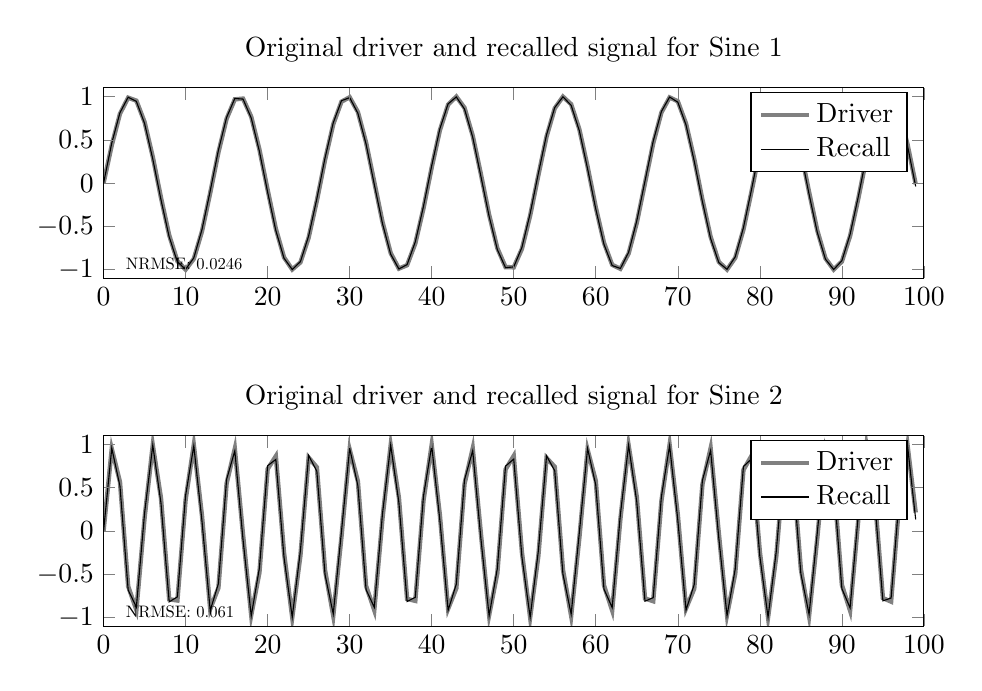
\begin{tikzpicture}

\begin{groupplot}[group style={group size=1 by 2,  vertical sep=2cm}]
\nextgroupplot[
title={Original driver and recalled signal for Sine 1},
xmin=0, xmax=100,
ymin=-1.1, ymax=1.1,
axis on top,
width=12cm,
height=4cm,
legend entries={{Driver},{Recall}},
legend cell align={left}
]
\addplot [ultra thick, white!50.196078431372548!black]
table {%
0 -4.3159920082303e-15
1 0.437292180580096
2 0.800951053453537
3 0.986328332143104
4 0.95207602432479
5 0.705840034997989
6 0.302441705019906
7 -0.168297531687922
8 -0.601563980086507
9 -0.900887106224276
10 -0.999620114586835
11 -0.875779259770038
12 -0.55693875602145
13 -0.114091134029353
14 0.35415984258038
15 0.743554138884904
16 0.967389825836667
17 0.975827997141108
18 0.76698982268473
19 0.387374885933405
20 -0.0784923410797969
21 -0.526882585376794
22 -0.857957971798231
23 -0.998001769174573
24 -0.915832043159276
25 -0.629744577284951
26 -0.203439162227017
27 0.26816370062171
28 0.680057650519136
29 0.940531020514899
30 0.991587214726886
31 0.821858140274661
32 0.469135409178337
33 0.0119557167406314
34 -0.447886017011694
35 -0.808002146068615
36 -0.988209772624168
37 -0.948384146526781
38 -0.69739277980872
39 -0.291121020233883
40 0.17997129340976
41 0.610991478472896
42 0.905969250198404
43 0.999225316222351
44 0.869995425769948
45 0.547053705472945
46 0.102305857038377
47 -0.365221254578165
48 -0.751428769071693
49 -0.970324321291476
50 -0.973168967664552
51 -0.759329323649045
52 -0.376418592152193
53 0.0903049182553011
54 0.536921275865156
55 0.863987576371796
56 0.998679745446811
57 0.911007433986741
58 0.620491622650302
59 0.191818110633478
60 -0.279565323881228
61 -0.688701177723657
62 -0.944491897325966
63 -0.989983518467513
64 -0.815046947462399
65 -0.458633289422644
66 -0.00010105570982366
67 0.458453678910341
68 0.814929829655062
69 0.989954970634164
70 0.944558275882825
71 0.688847702924381
72 0.279759370652273
73 -0.191619748444672
74 -0.62033311206052
75 -0.910924068717631
76 -0.998690087479674
77 -0.864089322965662
78 -0.537091772281518
79 -0.0905062020269657
80 0.376231338557086
81 0.759197793825064
82 0.973122447837935
83 0.970373169494652
84 0.751562108839202
85 0.36540939668615
86 -0.102104804025387
87 -0.546884507684024
88 -0.869895756605639
89 -0.999217367551436
90 -0.906054793025844
91 -0.611151461613133
92 -0.180170111509123
93 0.290927696327129
94 0.697247769048558
95 0.948320581148155
96 0.988238654784717
97 0.808128805390191
98 0.448038361021977
99 -0.0116478063828948
};
\addplot [black]
table {%
0 -0.000863353897974581
1 0.462587525584818
2 0.813546947339687
3 0.992182011181864
4 0.943491539833919
5 0.689499773637588
6 0.277810477322992
7 -0.192271604815125
8 -0.622858150357369
9 -0.909349711756128
10 -0.997238035864405
11 -0.864171020181012
12 -0.536602161965906
13 -0.0914559334373509
14 0.37975338473415
15 0.75883412778027
16 0.977749223395503
17 0.970684850631215
18 0.751764095985597
19 0.365902049804302
20 -0.104702437233319
21 -0.54844178823503
22 -0.86848308327281
23 -0.998433326125203
24 -0.906769504966375
25 -0.610788509584784
26 -0.181205932761363
27 0.291224097207164
28 0.696719054500838
29 0.951392431220541
30 0.987357203773641
31 0.807535796290414
32 0.451077510675316
33 -0.0145734395834164
34 -0.468124015714018
35 -0.821673474704589
36 -0.992196919163878
37 -0.9414608840534
38 -0.679061228464078
39 -0.268071018097352
40 0.200786620294783
41 0.628886238673769
42 0.915391601761463
43 0.995125201727666
44 0.855629908176208
45 0.530502264247751
46 0.0764216339329565
47 -0.383790527225668
48 -0.768154977539847
49 -0.97731732971701
50 -0.96822820207664
51 -0.742241109405759
52 -0.352381339186717
53 0.111735351120704
54 0.557987855157428
55 0.873455857073151
56 0.997200376936149
57 0.897676665854462
58 0.603954212585663
59 0.166191997146316
60 -0.299143567252587
61 -0.707901965579571
62 -0.952570255192714
63 -0.986223619080061
64 -0.800111272786251
65 -0.435346628500322
66 0.0229717923211878
67 0.483393776877081
68 0.82686894241965
69 0.994211847255461
70 0.934730068691118
71 0.67215715009064
72 0.254405773563454
73 -0.214940076225097
74 -0.641526792726654
75 -0.919261587876987
76 -0.995830761397464
77 -0.851631798389572
78 -0.515942839480604
79 -0.067376026503545
80 0.402395660128225
81 0.774083523525932
82 0.982731017097059
83 0.964467135476592
84 0.735774524158531
85 0.342634901421652
86 -0.128260396301783
87 -0.56880375119126
88 -0.879877713150755
89 -0.998786150795239
90 -0.896217933354009
91 -0.591693475433574
92 -0.157622244521334
93 0.31509138681174
94 0.713877228528922
95 0.959487195510634
96 0.98392841381306
97 0.793488504083945
98 0.428976457228872
99 -0.0386460793770816
};
\node at (axis cs:2,-1)[
  scale=0.6,
  anchor=base west,
  text=black,
  rotate=0.0
]{ NRMSE: 0.0246};
\nextgroupplot[
title={Original driver and recalled signal for Sine 2},
xmin=0, xmax=100,
ymin=-1.1, ymax=1.1,
axis on top,
width=12cm,
height=4cm,
legend entries={{Driver},{Recall}},
legend cell align={left}
]
\addplot [ultra thick, white!50.196078431372548!black]
table {%
0 7.7715611723761e-16
1 0.949548143847319
2 0.567846977221009
3 -0.638856767628373
4 -0.911741716234774
5 0.151062336306042
6 0.992513765853606
7 0.380495342122591
8 -0.788755121987039
9 -0.80289716489047
10 0.358776678210544
11 0.995034029517126
12 0.174096663753397
13 -0.901799538065081
14 -0.657039925033148
15 0.549933089076137
16 0.951547147805787
17 -0.0403483529146868
18 -0.973155015409511
19 -0.480808105646173
20 0.715666490332225
21 0.864071005913833
22 -0.252928099982759
23 -0.999522306859168
24 -0.282348908768776
25 0.848315196949918
26 0.736649546168949
27 -0.453815181426954
28 -0.979682474171906
29 -0.0708369455964804
30 0.941746964291059
31 0.575173361689677
32 -0.633722746676283
33 -0.914552697089022
34 0.143949753433392
35 0.99164251579499
36 0.38710736851674
37 -0.784333811563631
38 -0.807143873590579
39 0.352081769440307
40 0.99569521965724
41 0.181145708474725
42 -0.898685745916513
43 -0.662421428466841
44 0.543937324266117
45 0.953717722589972
46 -0.0331901741145079
47 -0.971492150432199
48 -0.487075765665267
49 0.710647087654222
50 0.867650611015999
51 -0.2459917012572
52 -0.999387242728024
53 -0.289212976218059
54 0.844504199358445
55 0.741472699296343
56 -0.447421226995936
57 -0.981081454793654
58 -0.0779801000777288
59 0.939320551184687
60 0.581017092295491
61 -0.628166823986022
62 -0.917421048698191
63 0.136857734290988
64 0.990712858328725
65 0.393701525566133
66 -0.779872766517105
67 -0.811348994565415
68 0.345368744061379
69 0.996305295159004
70 0.188185449313083
71 -0.895525809090902
72 -0.667768919397173
73 0.537913630493947
74 0.955839327752795
75 -0.0260302911272434
76 -0.96977940320274
77 -0.493318416283192
78 0.705591196078181
79 0.871185665714614
80 -0.239042671837653
81 -0.999200864040885
82 -0.296062193736209
83 0.840649839852298
84 0.74625778070525
85 -0.441004299087037
86 -0.982430061460068
87 -0.085119248089332
88 0.93684589837085
89 0.586831024836519
90 -0.622578777489712
91 -0.920241809003845
92 0.129756876563362
93 0.989739092258662
94 0.40025023687085
95 -0.775277515709292
96 -0.815863874862848
97 0.339949498422212
98 0.991969581016215
99 0.213482547869453
};
\addplot [black]
table {%
0 0.00017780355972867
1 0.957130058247109
2 0.51788604048634
3 -0.682045341190153
4 -0.87835056548317
5 0.20540178075365
6 0.99155348442546
7 0.321700411225028
8 -0.818733287614626
9 -0.761034316511022
10 0.411155390561632
11 0.983587582127827
12 0.112214106128835
13 -0.918403301622129
14 -0.607926887267749
15 0.597068882141646
16 0.925243812702757
17 -0.0991181472945674
18 -0.98082315562342
19 -0.426168848463918
20 0.754458429307742
21 0.826687834554244
22 -0.30667394618081
23 -0.995485482022961
24 -0.223326137567491
25 0.871709651718855
26 0.690439701748638
27 -0.505956529161653
28 -0.958119130016623
29 -0.00680184207292184
30 0.955169724142346
31 0.523894472308282
32 -0.676955662753053
33 -0.881505665181737
34 0.198645219824366
35 0.991047621258103
36 0.328465737737776
37 -0.814817006640027
38 -0.765522774292302
39 0.404570650278614
40 0.984661408958222
41 0.119167007066289
42 -0.915689244271438
43 -0.613403507681857
44 0.591428866955767
45 0.92785484386279
46 -0.0922336476627602
47 -0.979474536748337
48 -0.432588757325317
49 0.749828219594908
50 0.830560223215299
51 -0.299860246342926
52 -0.99585761562445
53 -0.230270811837425
54 0.868426889566502
55 0.695424648927775
56 -0.4997911861563
57 -0.960046166826741
58 -0.0138234929850887
59 0.953141898004518
60 0.529882954432473
61 -0.671818058318206
62 -0.884623061870612
63 0.191884218877516
64 0.990500863411992
65 0.335232207450927
66 -0.810850344556203
67 -0.769980766728153
68 0.397947642853422
69 0.985679748429494
70 0.126132880117691
71 -0.912932024988926
72 -0.618864060054956
73 0.585745745805001
74 0.930431862324521
75 -0.08532541514152
76 -0.978070258372598
77 -0.439001319322377
78 0.745137430419792
79 0.834397389168123
80 -0.293027059595129
81 -0.996170225990632
82 -0.237207794136846
83 0.865109091179134
84 0.700390427173873
85 -0.493577730442131
86 -0.961937082727547
87 -0.0208853541004996
88 0.951046814075153
89 0.535849725022037
90 -0.666633702523991
91 -0.887702170428038
92 0.185120230327716
93 0.98991371399832
94 0.341997472920758
95 -0.806834137873168
96 -0.774406701350748
97 0.391288594135441
98 0.986641973580973
99 0.133110069391768
};
\node at (axis cs:2,-1)[
  scale=0.6,
  anchor=base west,
  text=black,
  rotate=0.0
]{ NRMSE: 0.061};
\end{groupplot}

\end{tikzpicture}
	      	\caption[Successful loading of both sine patterns in RFC]{Successful loading of both sine patterns into the random feature conceptor architecture. The NRMSE between the original driver and the phase shifted, retrieved version of the pattern is on the order of $10^{-2}$ for both patterns. There is almost distinction visible to the eye between driver and recall.}
	   	    \label{loading}
	    \end{figure}
	
	So far we have seen the setup of one module of the random feature conceptor architecture with two sinewaves of different periods learned. In order to build a hierarchical random feature conceptor system, we bi-directionally connect three copies of this architecture. The resulting top-down and bottom-up pathways operate as it was introduced in the preceding chapter. 
	
	
    % general setup of the simulation experiment
    In addition to this we introduced a feedback loop from the top level hypothesis to the input of the system. This feedback loop suppresses those parts of the input signal that can be explained or predicted under the current hypothesis of the system.
     
    Let us first introduce the composition of the input pattern, without the effect of the feedback loop.
    
    \paragraph{Stimuli for binocular rivalry condition}
    The basis for the input to the system are the following two sinewaves that were mentioned earlier, with different periods, sampled at integer $n$:
    \begin{equation}
		s_1(n) = sin(\frac{2 \pi n}{13.1900453})
	\end{equation}
	\begin{equation}
		s_2(n) = sin(\frac{2 \pi n}{4.8342522})
	\end{equation}
	
	Furthermore a component of normally distributed noise, with the signal to noise ratio of 0.5 with respect to the clean sinewave input, is added. The noise was found to be necessary to push the system into an oscillating regime.  Figure \ref{input_without_feedback} shows the components and the resulting input pattern.
	
    \begin{figure}
    \centering
    % This file was created by matplotlib2tikz v0.5.4.
% The lastest updates can be retrieved from
% 
% https://github.com/nschloe/matplotlib2tikz
% 
% where you can also submit bug reports and leavecomments.
% 
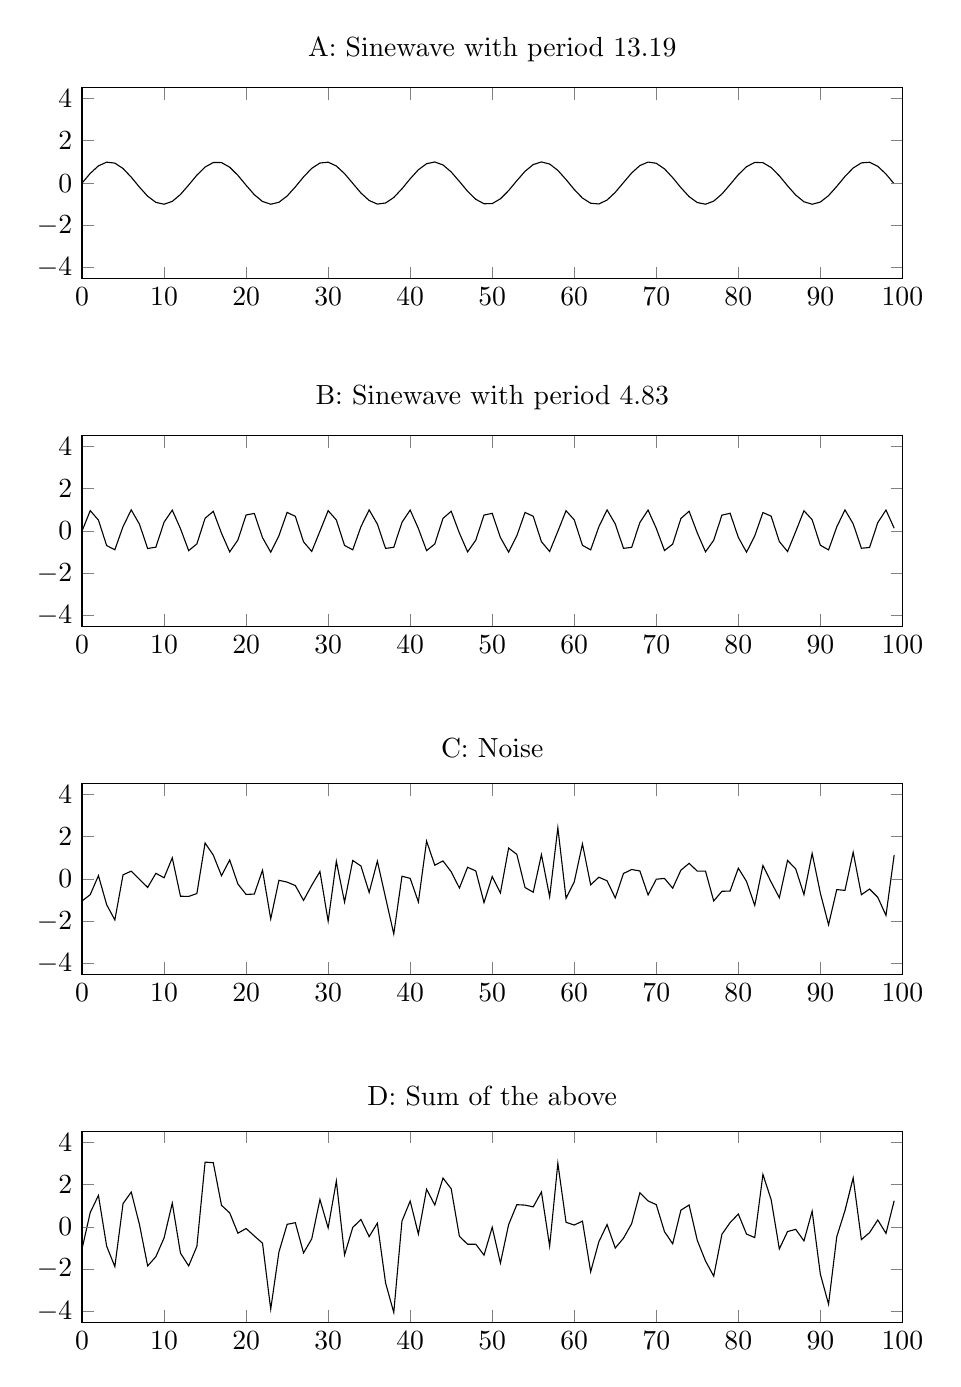
\begin{tikzpicture}

\begin{groupplot}[group style={group size=1 by 4, vertical sep=2cm}]
\nextgroupplot[
title={A: Sinewave with period 13.19},
xmin=0, xmax=100,
ymin=-4.5, ymax=4.5,
axis on top,
width=12cm,
height=4cm
]
\addplot [black]
table {%
0 0
1 0.458545799706575
2 0.814992504064339
3 0.989974243669887
4 0.944529856240803
5 0.688777918477953
6 0.279663759497863
7 -0.191719897675974
8 -0.620415500296462
9 -0.910970351521599
10 -0.998689959594449
11 -0.864042812865966
12 -0.537009235833885
13 -0.0904060166686075
14 0.376326865709943
15 0.759267392844971
16 0.973150621915276
17 0.970353645433025
18 0.751499233836268
19 0.365317170390766
20 -0.102205846643565
21 -0.546971868655055
22 -0.869949984187704
23 -0.999226387827859
24 -0.906016596389644
25 -0.611074557220486
26 -0.180071606528835
27 0.291025808306561
28 0.697323868812969
29 0.948356880077851
30 0.988230221827215
31 0.808065757735859
32 0.447978627468135
33 -0.0118547279953424
34 -0.469048528141322
35 -0.821804711742642
36 -0.991579135013796
37 -0.940570088637101
38 -0.680135167629238
39 -0.268262406880412
40 0.20334124460193
41 0.629669250479745
42 0.915796079323372
43 0.998013175959798
44 0.858014209387508
45 0.526971131995867
46 0.0785934810760336
47 -0.38728367223443
48 -0.766928844783529
49 -0.975810832282383
50 -0.967420295921345
51 -0.743625459490712
52 -0.354256133574122
53 0.113991312658539
54 0.556857630315804
55 0.875734893161736
56 0.999622385270665
57 0.900935510125847
58 0.601647734023414
59 0.168398008205687
60 -0.302346956489691
61 -0.705771817590585
62 -0.952050622300174
63 -0.98634731458976
64 -0.801025446238763
65 -0.437348496531251
66 0.0237077899329774
67 0.479485336724033
68 0.828501423386417
69 0.993044670308292
70 0.936478133770559
71 0.671396830914826
72 0.256823352794752
73 -0.214934014048256
74 -0.638834507252786
75 -0.920493101589524
76 -0.99719613203875
77 -0.851865021009328
78 -0.516858967891241
79 -0.0667698999938462
80 0.398186050099959
81 0.774482512915207
82 0.978333902669675
83 0.96435098563175
84 0.735647176384713
85 0.343145309772749
86 -0.125760758389869
87 -0.566665131475998
88 -0.881396726779768
89 -0.999877896269579
90 -0.895727806823594
91 -0.592136355546397
92 -0.15670074330836
93 0.313625612978591
94 0.714120577540189
95 0.95561056379104
96 0.984325786580392
97 0.793872559015008
98 0.42665690084936
99 -0.0355575199893448
};
\nextgroupplot[
title={B: Sinewave with period 4.83},
xmin=0, xmax=100,
ymin=-4.5, ymax=4.5,
axis on top,
width=12cm,
height=4cm
]
\addplot [black]
table {%
0 0
1 0.963483859354258
2 0.515977237002469
3 -0.687161109865611
4 -0.883974570223639
5 0.213763707411842
6 0.998452053215092
7 0.32094014537781
8 -0.826578069185718
9 -0.763599837249686
10 0.417645288034933
11 0.987262599915782
12 0.111066245173137
13 -0.927782979419511
14 -0.60792448894241
15 0.602219457970512
16 0.930432779014863
17 -0.103942159527367
18 -0.986097217770427
19 -0.424145273283411
20 0.758953499615038
21 0.830589788095706
22 -0.314145400565695
23 -0.998824963212765
24 -0.220758157770011
25 0.88060172243293
26 0.692349289504258
27 -0.509825948691939
28 -0.965377822161294
29 -0.00716556757080863
30 0.961540425487911
31 0.522102031936647
32 -0.68193764724044
33 -0.887302029440405
34 0.206758281138568
35 0.998027876680606
36 0.327718411191531
37 -0.822523908783549
38 -0.768206967073566
39 0.411123858364101
40 0.988377290058192
41 0.118184628009519
42 -0.925085541862862
43 -0.613598305412727
44 0.596483505427653
45 0.93303480459226
46 -0.0968127368656248
47 -0.984881203459862
48 -0.430623480361169
49 0.754268192740552
50 0.834558859527716
51 -0.307334525638279
52 -0.999146587526183
53 -0.227741273075896
54 0.877183659250578
55 0.697501919764026
56 -0.503648482849212
57 -0.967222216661571
58 -0.0143307672182578
59 0.959547620349843
60 0.528200019010654
61 -0.676679169832758
62 -0.890583929231452
63 0.199742238650924
64 0.997552455389084
65 0.334479849969908
66 -0.818427515054188
67 -0.772774652528905
68 0.404581319120358
69 0.989441230962756
70 0.125296942535891
71 -0.922340604847591
72 -0.619240616053586
73 0.590716925832167
74 0.935588922548051
75 -0.0896783432553982
76 -0.983614619421572
77 -0.437079576638072
78 0.749544157198085
79 0.83848507968575
80 -0.300507870306872
81 -0.999416909641218
82 -0.234712694774352
83 0.873720556180522
84 0.702618736077859
85 -0.497445156662569
86 -0.969016948152775
87 -0.0214952310378938
88 0.95750554626266
89 0.534270885117103
90 -0.671385947644433
91 -0.893820101084288
92 0.192715940194747
93 0.997025813751514
94 0.341224114539962
95 -0.814289098331132
96 -0.77730265908324
97 0.398018006237022
98 0.990454368000349
99 0.132402823563217
};
\nextgroupplot[
title={C: Noise},
xmin=0, xmax=100,
ymin=-4.5, ymax=4.5,
axis on top,
width=12cm,
height=4cm
]
\addplot [black]
table {%
0 -1.04211242578326
1 -0.743414460739167
2 0.155158481297336
3 -1.21486104145389
4 -1.938327304975
5 0.196172252396362
6 0.366400066503094
7 -0.0194710709215659
8 -0.400833661496304
9 0.265087357935895
10 0.0561783306910247
11 0.997585307676022
12 -0.817694749647003
13 -0.826446548382765
14 -0.690800439126271
15 1.69856095789247
16 1.12586836240051
17 0.151702913971487
18 0.895182647426236
19 -0.240816828412866
20 -0.733421828843349
21 -0.714096276127972
22 0.412945591901335
23 -1.89081401942814
24 -0.0647384425693875
25 -0.149850601919324
26 -0.313707560438835
27 -1.01245921354023
28 -0.30125586623724
29 0.350854861607519
30 -1.99684937367521
31 0.832719979278175
32 -1.09157933254277
33 0.873155776167019
34 0.609819329904048
35 -0.637555652846466
36 0.839159468166351
37 -0.884524499913894
38 -2.59701604455154
39 0.129014609840152
40 0.0270668778529112
41 -1.08829282084642
42 1.78690363945792
43 0.649126719974281
44 0.851039169083406
45 0.339874575188399
46 -0.430173968774262
47 0.550618906343835
48 0.378543902915821
49 -1.11657951124474
50 0.112768580548706
51 -0.660768414863171
52 1.4581561381085
53 1.16203536437436
54 -0.406607915690425
55 -0.627955425351646
56 1.15084704177296
57 -0.840989481099017
58 2.41771737173263
59 -0.913600287558711
60 -0.141588211898227
61 1.65404974706793
62 -0.279143869022234
63 0.0813643218415902
64 -0.0876818309240491
65 -0.897068423290958
66 0.25766665010864
67 0.446493103949885
68 0.376928493268927
69 -0.756213276762159
70 -0.0130596050546269
71 0.0244228611929558
72 -0.437644139185622
73 0.412727791566086
74 0.736496574605388
75 0.369091264750332
76 0.36992956860466
77 -1.04176449456228
78 -0.584999529728029
79 -0.570987725771648
80 0.508463446993452
81 -0.116702685228239
82 -1.25015445370133
83 0.638020659313296
84 -0.148524955692922
85 -0.889306859555434
86 0.873712557953627
87 0.470182886276912
88 -0.739455157663081
89 1.2070432864943
90 -0.669914816771898
91 -2.166237094752
92 -0.50254943998927
93 -0.542086060507473
94 1.26093404180405
95 -0.744293574869851
96 -0.477871669319
97 -0.868250923260022
98 -1.7237430854398
99 1.13749514226596
};
\nextgroupplot[
title={D: Sum of the above},
xmin=0, xmax=100,
ymin=-4.5, ymax=4.5,
axis on top,
width=12cm,
height=4cm
]
\addplot [black]
table {%
0 -1.04211242578326
1 0.678615198321666
2 1.48612822236414
3 -0.912047907649615
4 -1.87777201895784
5 1.09871387828616
6 1.64451587921605
7 0.10974917678027
8 -1.84782723097848
9 -1.40948283083539
10 -0.524866340868491
11 1.12080509472584
12 -1.24363774030775
13 -1.84463554447088
14 -0.922398062358738
15 3.06004780870795
16 3.02945176333065
17 1.01811439987715
18 0.660584663492077
19 -0.29964493130551
20 -0.0766741758718753
21 -0.430478356687321
22 -0.771149792852064
23 -3.88886537046876
24 -1.19151319672904
25 0.11967656329312
26 0.198570122536589
27 -1.2312593539256
28 -0.569309819585564
29 1.29204617411456
30 -0.0470787263600803
31 2.16288776895068
32 -1.32553835231507
33 -0.0260009812687287
34 0.347529082901294
35 -0.461332487908503
36 0.175298744344086
37 -2.64761849733454
38 -4.04535817925434
39 0.271876061323841
40 1.21878541251303
41 -0.340438942357154
42 1.77761417691843
43 1.03354159052135
44 2.30553688389857
45 1.79988051177653
46 -0.448393224563853
47 -0.821545969350457
48 -0.819008422228876
49 -1.33812215078657
50 -0.0200928558449233
51 -1.71172839999216
52 0.104753417008193
53 1.048285403957
54 1.02743337387596
55 0.945281387574116
56 1.64682094419441
57 -0.907276187634741
58 3.00503433853778
59 0.214345340996819
60 0.0842648506227356
61 0.271598759644588
62 -2.12177842055386
63 -0.705240754097247
64 0.108845178226271
65 -0.999937069852301
66 -0.537053075012571
67 0.153203788145013
68 1.6100112357757
69 1.22627262450889
70 1.04871547125182
71 -0.226520912739809
72 -0.800061402444456
73 0.788510703349997
74 1.03325098990065
75 -0.64108018009459
76 -1.61088118285566
77 -2.33070909220968
78 -0.352314340421185
79 0.200727453920256
80 0.606141626786539
81 -0.34163708195425
82 -0.506533245806004
83 2.47609220112557
84 1.28974095676965
85 -1.04360670644525
86 -0.221065148589018
87 -0.117977476236979
88 -0.66334633818019
89 0.741436275341819
90 -2.23702857123993
91 -3.65219355138268
92 -0.466534243102882
93 0.768565366222633
94 2.3162787338842
95 -0.602972109409943
96 -0.270848541821848
97 0.323639641992009
98 -0.306631816590091
99 1.23434044583983
};
\end{groupplot}

\end{tikzpicture}
    \caption[Binocular rivalry input, as it would be without the influence from the feedback loop.]{A sample of the binocular rivalry input, as it would be without the influence from the feedback loop. $A$ and $B$ show the familiar two sinewave patterns. $C$ shows a sample of normally distributed noise. $D$ shows the composed binocular rivalry input signal, effectively the sum of $A$, $B$ and $C$}.
    \label{input_without_feedback}
    \end{figure}	


	The effective input signal to the system is different most of the time, due to the effect of the feedback loop. When the system settles on a hypothesis, the part of the input signal that can be explained by that hypothesis is subtracted from the input. Importantly, we defined the winning hypothesis by the procedure of 'the winner takes it all'. Therefore there is a winning hypothesis at all points in time, except for the cases where 0.5 is assigned as probability to both hypotheses. If one hypothesis is only slightly more likely, for example 0.55, while the other is assigned 0.45, the first one is decided to be the leading hypothesis. This effects the input drastically, the complete clear signal that belongs to the winning hypothesis is subtracted. Thereby the effective input to the system is usually a composition of noise and one signal source. 
	
	 \begin{figure}
	 \centering
	     % This file was created by matplotlib2tikz v0.5.4.
% The lastest updates can be retrieved from
% 
% https://github.com/nschloe/matplotlib2tikz
% 
% where you can also submit bug reports and leavecomments.
% 
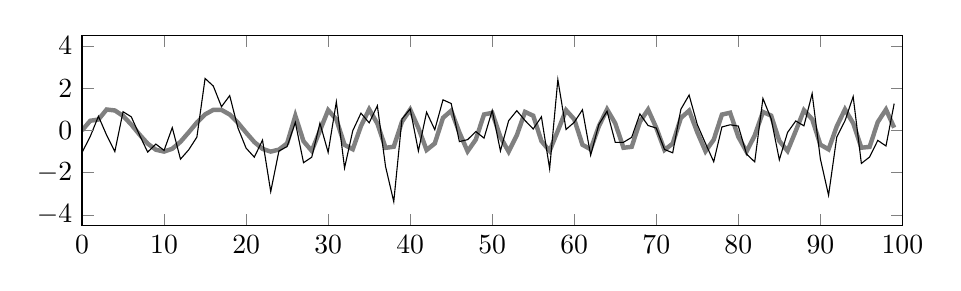
\begin{tikzpicture}

\begin{axis}[
xmin=0, xmax=100,
ymin=-4.5, ymax=4.5,
axis on top,
width=12cm,
height=4cm
]
\addplot [ultra thick, white!50.196078431372548!black]
table {%
0 0
1 0.458545799706575
2 0.515977237002469
3 0.989974243669887
4 0.944529856240803
5 0.688777918477953
6 0.279663759497863
7 -0.191719897675974
8 -0.620415500296462
9 -0.910970351521599
10 -0.998689959594449
11 -0.864042812865966
12 -0.537009235833885
13 -0.0904060166686075
14 0.376326865709943
15 0.759267392844971
16 0.973150621915276
17 0.970353645433025
18 0.751499233836268
19 0.365317170390766
20 -0.102205846643565
21 -0.546971868655055
22 -0.869949984187704
23 -0.999226387827859
24 -0.906016596389644
25 -0.611074557220486
26 0.692349289504258
27 -0.509825948691939
28 -0.965377822161294
29 -0.00716556757080863
30 0.961540425487911
31 0.522102031936647
32 -0.68193764724044
33 -0.887302029440405
34 0.206758281138568
35 0.998027876680606
36 0.327718411191531
37 -0.822523908783549
38 -0.768206967073566
39 0.411123858364101
40 0.988377290058192
41 0.118184628009519
42 -0.925085541862862
43 -0.613598305412727
44 0.596483505427653
45 0.93303480459226
46 -0.0968127368656248
47 -0.984881203459862
48 -0.430623480361169
49 0.754268192740552
50 0.834558859527716
51 -0.307334525638279
52 -0.999146587526183
53 -0.227741273075896
54 0.877183659250578
55 0.697501919764026
56 -0.503648482849212
57 -0.967222216661571
58 -0.0143307672182578
59 0.959547620349843
60 0.528200019010654
61 -0.676679169832758
62 -0.890583929231452
63 0.199742238650924
64 0.997552455389084
65 0.334479849969908
66 -0.818427515054188
67 -0.772774652528905
68 0.404581319120358
69 0.989441230962756
70 0.125296942535891
71 -0.922340604847591
72 -0.619240616053586
73 0.590716925832167
74 0.935588922548051
75 -0.0896783432553982
76 -0.983614619421572
77 -0.437079576638072
78 0.749544157198085
79 0.83848507968575
80 -0.300507870306872
81 -0.999416909641218
82 -0.234712694774352
83 0.873720556180522
84 0.702618736077859
85 -0.497445156662569
86 -0.969016948152775
87 -0.0214952310378938
88 0.95750554626266
89 0.534270885117103
90 -0.671385947644433
91 -0.893820101084288
92 0.192715940194747
93 0.997025813751514
94 0.341224114539962
95 -0.814289098331132
96 -0.77730265908324
97 0.398018006237022
98 0.990454368000349
99 0.132402823563217
};
\addplot [black]
table {%
0 -1.04211242578326
1 -0.284868661032593
2 0.671135718299805
3 -0.224886797784004
4 -0.993797448734198
5 0.884950170874314
6 0.646063826000956
7 -0.21119096859754
8 -1.02124916179277
9 -0.645882993585704
10 -0.942511628903424
11 0.133542494810056
12 -1.35470398548089
13 -0.916852565051372
14 -0.314473573416328
15 2.45782835073744
16 2.09901898431578
17 1.12205655940451
18 1.6466818812625
19 0.124500341977901
20 -0.835627675486914
21 -1.26106814478303
22 -0.457004392286369
23 -2.890040407256
24 -0.970755038959032
25 -0.76092515913981
26 0.378641729065424
27 -1.52228516223217
28 -1.26663368839853
29 0.34368929403671
30 -1.03530894818729
31 1.35482201121482
32 -1.77351697978321
33 -0.0141462532733864
34 0.816577611042617
35 0.36047222383414
36 1.16687787935788
37 -1.70704840869744
38 -3.3652230116251
39 0.540138468204253
40 1.0154441679111
41 -0.970108192836898
42 0.86181809759506
43 0.035528414561554
44 1.44752267451106
45 1.27290937978066
46 -0.526986705639887
47 -0.434262297116027
48 -0.0520795774453478
49 -0.362311318504188
50 0.947327440076422
51 -0.96810294050145
52 0.459009550582315
53 0.934294091298465
54 0.470575743560154
55 0.0695464944123793
56 0.647198558923745
57 -1.80821169776059
58 2.40338660451437
59 0.0459473327911318
60 0.386611807112427
61 0.977370577235174
62 -1.16972779825369
63 0.281106560492514
64 0.909870624465034
65 -0.56258857332105
66 -0.560760864945548
67 -0.32628154857902
68 0.781509812389284
69 0.233227954200597
70 0.112237337481264
71 -0.897917743654635
72 -1.05688475523921
73 1.00344471739825
74 1.67208549715344
75 0.279412921494934
76 -0.613685050816911
77 -1.47884407120035
78 0.164544627470056
79 0.267497353914102
80 0.20795557668658
81 -1.11611959486946
82 -1.48486714847568
83 1.51174121549382
84 0.554093780384937
85 -1.386752016218
86 -0.0953043901991485
87 0.448687655239018
88 0.218050388599578
89 1.7413141716114
90 -1.34130076441633
91 -3.06005719583629
92 -0.309833499794522
93 0.454939753244042
94 1.60215815634401
95 -1.55858267320098
96 -1.25517432840224
97 -0.470232917022999
98 -0.733288717439451
99 1.26989796582918
};
\end{axis}

\end{tikzpicture}
	 \caption[Effective binocular rivalry input, with influence from the feedback loop.]{A sample of the effective binocular rivalry input, with influence from the feedback loop. Up to timepoint 23 the signal consists of sinewave 1 and noise, thereafter of sinewave 2 plus noise. The hypothesis that sinewave 2 is the source in the signal was winning until timestep 23. Therefore the signal of sinewave 1, which is not predictable under this hypothesis, remained in the input signal. From timestep 23 on the same reasoning holds, with hypothesis 1 being the winning hypothesis and sinewave 2 remaining as unpredicted residuum in the input signal.}
	 \label{sample_binocular_input}
	 \end{figure}	
	
	 A sample of this effective input is shown in Figure \ref{sample_binocular_input}. 
	

   	The system is run for 50.000 timesteps. Over the course of this simulation the hypothesis of the system about the source of the driver is collected on all three levels of the hierarchy. Moreover the dynamics of the trust variables that operate between the levels are saved. The results and analysis of this simulation are detailed in the next section. 

%\end{methods}

\section{Results}
    \label{sec:results}	
	    \begin{figure}
	    	\centering
	    	     % This file was created by matplotlib2tikz v0.5.4.
% The lastest updates can be retrieved from
% 
% https://github.com/nschloe/matplotlib2tikz
% 
% where you can also submit bug reports and leavecomments.
% 
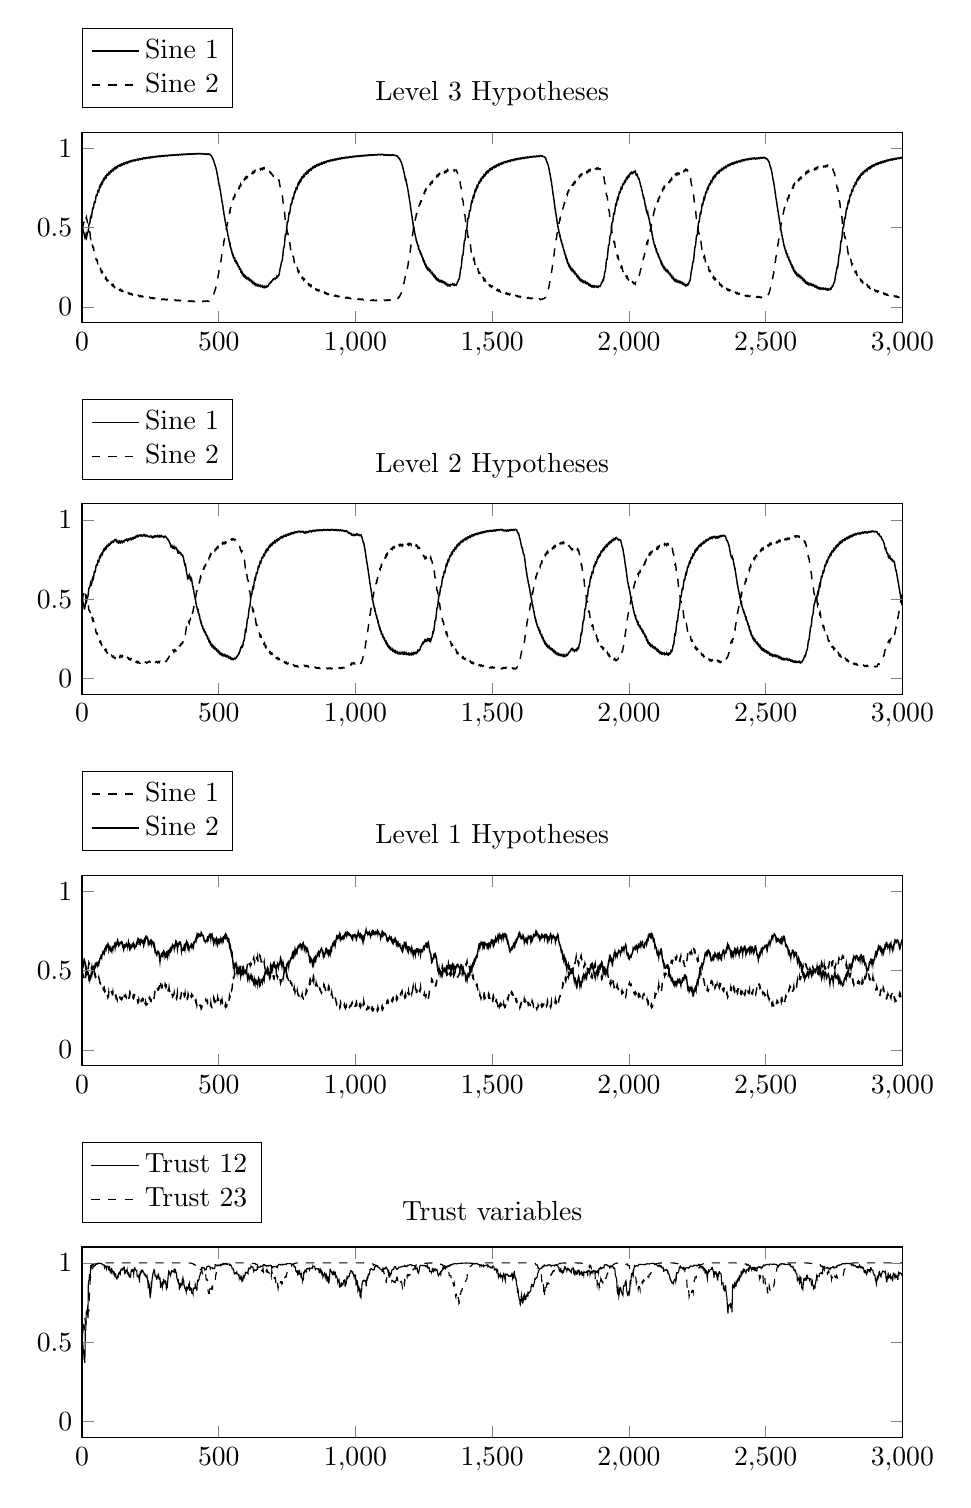
\begin{tikzpicture}

\begin{groupplot}[group style={group size=1 by 4, vertical sep=2.3cm}]
\nextgroupplot[
title={Level 3 Hypotheses},
xmin=0, xmax=3000,
ymin=-0.1, ymax=1.1,
axis on top,
width=12cm,
height=4cm,
legend style={at={(0.0,1.55)}, anchor=north west},
legend cell align={left},
legend entries={{Sine 1},{Sine 2}}
]
\addplot [line width=0.52pt, black]
table {%
0 0.499602113494523
1 0.505804108081564
2 0.499920772008212
3 0.492092294755299
4 0.482969530684502
5 0.476442882816674
6 0.469031172669856
7 0.467404641928024
8 0.456928493515095
9 0.444475782633752
10 0.442990194858059
11 0.43499108845279
12 0.44018975430213
13 0.443311600915671
14 0.452266727550768
15 0.43725221264353
16 0.433543367204006
17 0.442826922772513
18 0.450450113261335
19 0.45980688574883
20 0.46843732565825
21 0.470722776315622
22 0.472069413861411
23 0.482699195177809
24 0.498464027599486
25 0.515963645901422
26 0.523786693175984
27 0.523987602421179
28 0.525579244892468
29 0.534655003255182
30 0.549968051570145
31 0.565879040023242
32 0.570212319320694
33 0.56233241212704
34 0.561859916826807
35 0.570116919457147
36 0.585548186334896
37 0.599449922992957
38 0.613458691565334
39 0.623799202362009
40 0.625312922266183
41 0.621422912737461
42 0.624809110147846
43 0.637711070341092
44 0.651179414730098
45 0.660844351698867
46 0.659649929921152
47 0.656926584281487
48 0.659183568805672
49 0.670182375050779
50 0.682783756029425
51 0.695602708818037
52 0.704095340654542
53 0.705751971641096
54 0.701977848555672
55 0.702725651339711
56 0.712649516213747
57 0.724169563434369
58 0.733916514956062
59 0.733215810865636
60 0.728211444336844
61 0.727007078703645
62 0.734999469432861
63 0.745268862402981
64 0.755349105241237
65 0.763162663486075
66 0.766453170556474
67 0.762205458127146
68 0.759420036774259
69 0.765421964035462
70 0.774854059834493
71 0.783621124691302
72 0.785580350176627
73 0.780456420960428
74 0.776787735166858
75 0.780681592468957
76 0.788865264266396
77 0.796926221075505
78 0.804236781448984
79 0.807792294644896
80 0.805145567375243
81 0.801081363131
82 0.803031775252913
83 0.810502254863181
84 0.817662787766642
85 0.821019126834683
86 0.816503505283149
87 0.812078612113999
88 0.813204093066295
89 0.819672291844462
90 0.826549289093793
91 0.8331123068878
92 0.836563655629053
93 0.835089504229457
94 0.830730701833218
95 0.830556896783254
96 0.836540774933642
97 0.84273559993697
98 0.846869716143425
99 0.843690965609974
100 0.839169126627309
101 0.838325159069657
102 0.843350015504808
103 0.849325723202896
104 0.855169062554859
105 0.858705304592657
106 0.8584451730332
107 0.854158758563597
108 0.852438937163773
109 0.856887469739954
110 0.862493561798312
111 0.867195395470177
112 0.865803862782589
113 0.86128642630873
114 0.858890710623994
115 0.862303234210452
116 0.867465044740919
117 0.87251748241296
118 0.876351130725581
119 0.877382950226513
120 0.873738087196831
121 0.870712652601103
122 0.87315042068017
123 0.878092766051578
124 0.882698031718919
125 0.883340628865265
126 0.879109745465072
127 0.875654390823999
128 0.876991629129991
129 0.881348141477048
130 0.885679586039085
131 0.88959782854491
132 0.891183850281869
133 0.888904369272055
134 0.885430057725962
135 0.885668554734969
136 0.88978233706271
137 0.893727967250497
138 0.895361489114617
139 0.891807149895679
140 0.888194740413256
141 0.888120740051169
142 0.891755092146031
143 0.895743466567038
144 0.899561417458678
145 0.901360821123542
146 0.899930222937482
147 0.896427698217594
148 0.895646738920843
149 0.899128619115018
150 0.902848217774057
151 0.905313067112776
152 0.902848616791221
153 0.899259875769303
154 0.898028974127383
155 0.900939522297083
156 0.904598127546488
157 0.9081865310909
158 0.910286890568468
159 0.909877165427612
160 0.906527354982378
161 0.904761636576823
162 0.907344609407173
163 0.910897988209322
164 0.913907108131749
165 0.912813310705085
166 0.909267215390529
167 0.907067737206958
168 0.908964418189528
169 0.912267197676188
170 0.915493197854659
171 0.91798692577286
172 0.918552686151175
173 0.915779102351044
174 0.913211088642242
175 0.914431179985234
176 0.917664473938162
177 0.920692871792005
178 0.921112112892436
179 0.917862518901296
180 0.915025185926326
181 0.915534353316612
182 0.918398515458347
183 0.921299974022933
184 0.923943446794603
185 0.924917249241482
186 0.923155502435463
187 0.920354886888597
188 0.920133857022349
189 0.922898960337824
190 0.925576503914679
191 0.926677446592883
192 0.923927506259341
193 0.921023268609334
194 0.920624713008648
195 0.923083140566198
196 0.925860804292612
197 0.928534539785303
198 0.929751832609222
199 0.928609106237884
200 0.925792248125039
201 0.924918814175792
202 0.927309978834493
203 0.929958861823355
204 0.931771146284863
205 0.929909754538989
206 0.927023399011291
207 0.925785716761719
208 0.92775472094614
209 0.930367128576442
210 0.932938640642886
211 0.934459865276319
212 0.934151357270042
213 0.931482457135509
214 0.929852454187485
215 0.93156627212362
216 0.934160259026207
217 0.936398267302258
218 0.935629314402359
219 0.932759986556077
220 0.930807952590758
221 0.931987459218784
222 0.934397312496197
223 0.936744981629997
224 0.938622516105594
225 0.939042766005358
226 0.936891827123966
227 0.934705716419258
228 0.935339228807827
229 0.937720113969757
230 0.939961873206389
231 0.940342171951676
232 0.937751963392603
233 0.935378236835551
234 0.935524972376885
235 0.937637745796067
236 0.939825508214186
237 0.941836776582595
238 0.942549612429344
239 0.941159232083609
240 0.938832536539917
241 0.938447242549204
242 0.940517023010855
243 0.942555058629753
244 0.94344552306356
245 0.941256086924773
246 0.938837930309081
247 0.938313639091813
248 0.940150361223002
249 0.942287306707276
250 0.944354638293394
251 0.945299833744635
252 0.944407836449527
253 0.942063131433604
254 0.941182789315397
255 0.942973530171582
256 0.945043863347176
257 0.946523633808007
258 0.945088098557467
259 0.942678103221039
260 0.94149127177193
261 0.942937354803004
262 0.944971011691153
263 0.946977409660952
264 0.94820558746475
265 0.948012469382874
266 0.945814504216945
267 0.944314591467919
268 0.945528499145422
269 0.947577191133911
270 0.949380654294563
271 0.948869140011831
272 0.946467689401376
273 0.944712293774536
274 0.945473244357614
275 0.947366487722452
276 0.949209855769547
277 0.950737627800206
278 0.951094143476739
279 0.949383943933998
280 0.947483225023294
281 0.947775111615151
282 0.94965174302497
283 0.95142409193779
284 0.951787557135869
285 0.949642134863678
286 0.947604596559621
287 0.947566927935982
288 0.949237254873558
289 0.951005789043502
290 0.952647453034767
291 0.953224229069954
292 0.952089168124126
293 0.950095467263384
294 0.949649565008556
295 0.951304178731744
296 0.952968427614791
297 0.953760574535881
298 0.95197231999017
299 0.949895379092914
300 0.949312568430206
301 0.950768793603978
302 0.952514125407177
303 0.954209578860864
304 0.955002786231104
305 0.954306448173978
306 0.952297273225746
307 0.951427529171622
308 0.952838245019968
309 0.954550782211208
310 0.955828610437804
311 0.954697621568348
312 0.952620259378947
313 0.951489956817489
314 0.952603688958218
315 0.954274948072622
316 0.955924331813851
317 0.956980664993772
318 0.956881389217621
319 0.955022914485029
320 0.953632978614025
321 0.954521284528484
322 0.956219367707745
323 0.957741420046849
324 0.957423031091325
325 0.955361586345318
326 0.953762080337889
327 0.954251746975803
328 0.955809545909061
329 0.957332175261171
330 0.958632718643038
331 0.958951472130592
332 0.957558892721261
333 0.955875123380613
334 0.955952847761007
335 0.957498871553708
336 0.958961239367183
337 0.959304347678811
338 0.957470042062879
339 0.955681743039174
340 0.955542467939747
341 0.956924983073475
342 0.958419645208515
343 0.959820905833209
344 0.960318062192569
345 0.959363970520754
346 0.957611963222561
347 0.95714687799237
348 0.958528256648945
349 0.959950322358266
350 0.960688045716585
351 0.959198078935717
352 0.957371550125522
353 0.956759576101705
354 0.957959590076945
355 0.959441955186174
356 0.960887484669673
357 0.961585574679448
358 0.961040037083708
359 0.959279997968846
360 0.958424801429913
361 0.959572597477236
362 0.961043638729566
363 0.962183971718474
364 0.961279003953298
365 0.959443321762687
366 0.958364255979973
367 0.959246589455778
368 0.960671628364749
369 0.962075833644525
370 0.96302036666134
371 0.962992020545529
372 0.961389920218244
373 0.960092625498804
374 0.960750453149419
375 0.962204090123316
376 0.963526782493833
377 0.963351596819766
378 0.961548412476829
379 0.960076521505899
380 0.960379968985877
381 0.961703094446777
382 0.963008158055731
383 0.964148860224069
384 0.964441196437008
385 0.963281066033143
386 0.961765986898819
387 0.961704842711805
388 0.963018899836166
389 0.964263653948138
390 0.964582113173309
391 0.962973199827805
392 0.96137613558608
393 0.961175575953945
394 0.962355876820703
395 0.963656388794761
396 0.964884976781376
397 0.965328198625177
398 0.964509127209207
399 0.962939722525897
400 0.962463526231703
401 0.963645230943971
402 0.964885514788696
403 0.965580044518725
404 0.9643407814819
405 0.96272156538783
406 0.962078518747927
407 0.963077862360812
408 0.964362879986463
409 0.96561697750253
410 0.966259788202039
411 0.965895213823112
412 0.964334833221119
413 0.963437350592899
414 0.964339108578301
415 0.965582792613106
416 0.966556328615632
417 0.965972751654806
418 0.964530224372132
419 0.963359634279269
420 0.963858999445258
421 0.964973341401612
422 0.966215558280883
423 0.967107741627239
424 0.96723820267055
425 0.966082981025043
426 0.964808661744516
427 0.965008651576973
428 0.96619728429786
429 0.967153934994324
430 0.966686858635214
431 0.96509803494521
432 0.963803580543524
433 0.963786092317654
434 0.96478754377018
435 0.965893297645425
436 0.96690569885108
437 0.966990531431899
438 0.965984695678048
439 0.964708299791993
440 0.964457552397056
441 0.965515004306411
442 0.966464778386133
443 0.96584348423529
444 0.96371927719341
445 0.962351236236393
446 0.962266375954686
447 0.963284086373462
448 0.964268126899239
449 0.965309977839308
450 0.965863561830334
451 0.964783574320127
452 0.963001762450362
453 0.962422154375186
454 0.963187796304882
455 0.96386798245244
456 0.964848297887998
457 0.965092944594887
458 0.963913109138732
459 0.962125250339059
460 0.962112020679962
461 0.962771551252278
462 0.96377022576712
463 0.964536066260748
464 0.96504844672891
465 0.963993636251009
466 0.961878395517418
467 0.961001165070085
468 0.959865629672654
469 0.957903553138202
470 0.957568999885221
471 0.956717652400927
472 0.954352990053728
473 0.950944974404101
474 0.95007094845561
475 0.946653310064989
476 0.942661792657757
477 0.938275015336474
478 0.935065367261457
479 0.932375486109978
480 0.925753023659058
481 0.923345906579447
482 0.919125809093555
483 0.912070619113036
484 0.907286370898726
485 0.900457791937181
486 0.896172549016614
487 0.888461678399648
488 0.885321659344381
489 0.88122058411624
490 0.872360487037996
491 0.867078449931254
492 0.856339325473233
493 0.850231737536198
494 0.83898526279862
495 0.830443914467809
496 0.825029805248124
497 0.809843418177625
498 0.803689492807837
499 0.791718350127729
500 0.78257707442744
501 0.770127541628188
502 0.763130879518769
503 0.763772808452166
504 0.747553893415184
505 0.739375800246447
506 0.732855024587044
507 0.718340709461474
508 0.711180590385361
509 0.695826515648287
510 0.689279569115508
511 0.672673530517916
512 0.662735118813342
513 0.659454716442035
514 0.642986083408307
515 0.638135489957163
516 0.6195131128585
517 0.611339905501806
518 0.60257671535868
519 0.584595248940252
520 0.582637313486126
521 0.564998554214876
522 0.555936574725622
523 0.54749765956531
524 0.534736430645577
525 0.532338416193434
526 0.516401688004707
527 0.513948318590968
528 0.505582401315783
529 0.492187365603562
530 0.48990376972194
531 0.473646467453485
532 0.470897775245658
533 0.457425332025335
534 0.44877580648537
535 0.444202485112208
536 0.428617547720038
537 0.42823727717477
538 0.414741518886089
539 0.408785935389571
540 0.396913277072541
541 0.388548895945416
542 0.392244456969224
543 0.376647059112889
544 0.374965881652681
545 0.365831673668641
546 0.356578194786904
547 0.356735820465554
548 0.343783081986749
549 0.343579452244479
550 0.33009168400519
551 0.326216235435867
552 0.328371811547674
553 0.317433506766158
554 0.319323942996063
555 0.310486258393122
556 0.306080388608888
557 0.304769922809061
558 0.297099084943788
559 0.300918214345587
560 0.291484952313379
561 0.290030344419648
562 0.288709190942161
563 0.282098082681246
564 0.285101749408328
565 0.276475096049146
566 0.276880993376435
567 0.274709296307102
568 0.267768219660389
569 0.270894253453682
570 0.26171895814532
571 0.262351344549011
572 0.257610633330176
573 0.252722556937757
574 0.252964489825617
575 0.244138414162405
576 0.246849849612376
577 0.239383409327015
578 0.236834427119499
579 0.233350955248821
580 0.226986059161945
581 0.231112331707471
582 0.221975083709273
583 0.221760009215127
584 0.215165795133151
585 0.21094355235393
586 0.214989560254279
587 0.206628298090718
588 0.208208593509314
589 0.201848330601249
590 0.198581781785853
591 0.20126193699297
592 0.19466514959758
593 0.19711967844988
594 0.190401944930659
595 0.189335794737079
596 0.191617706312354
597 0.186235556263246
598 0.190022643094744
599 0.185072822308751
600 0.184171633187773
601 0.184642410627391
602 0.180719635567283
603 0.185190761073441
604 0.179945213568688
605 0.180172169122466
606 0.180352905971561
607 0.176596748142271
608 0.180256013729111
609 0.174640070569061
610 0.176258084893348
611 0.175442304926513
612 0.171605322783445
613 0.174635104328254
614 0.168662942566465
615 0.170764088087051
616 0.167514747260691
617 0.165268923104209
618 0.165806903998555
619 0.160484971269954
620 0.163651212992536
621 0.158244426875183
622 0.157975260027976
623 0.155111422278865
624 0.151825731026131
625 0.155956530538014
626 0.149970772295633
627 0.151302396765057
628 0.14694370168291
629 0.144749598666745
630 0.148195267469159
631 0.142948012002313
632 0.144905483930449
633 0.14040540363605
634 0.139130661113794
635 0.141616051949198
636 0.137388125627353
637 0.140467392985194
638 0.136282572642453
639 0.135975612727525
640 0.137710926930635
641 0.134762195047283
642 0.138337584547378
643 0.134671955582262
644 0.135498018554835
645 0.136129844007618
646 0.133465403694482
647 0.137497713126922
648 0.13401019778483
649 0.1348474561353
650 0.134177182327795
651 0.131955670795899
652 0.13468669756849
653 0.130288930274964
654 0.132607076829972
655 0.131782292236377
656 0.130499726036613
657 0.130755616896212
658 0.128448449623939
659 0.131960057868912
660 0.127184648343483
661 0.128894038268701
662 0.128544913497352
663 0.12603353956681
664 0.128093147040413
665 0.124495566405782
666 0.127053552061964
667 0.121770588658636
668 0.122685361866431
669 0.126780444780162
670 0.124365012088962
671 0.126782515321392
672 0.12465646396461
673 0.125766545537393
674 0.126292299214957
675 0.125261956191116
676 0.130950644824875
677 0.128279561897228
678 0.127835271696822
679 0.129387015957623
680 0.130503898903959
681 0.134275512332624
682 0.136495385038479
683 0.143536557060739
684 0.144891692687243
685 0.145146858802946
686 0.147894858991419
687 0.148539039922799
688 0.1529411941787
689 0.152413910422228
690 0.156637386098735
691 0.154855765311522
692 0.155899053974321
693 0.160859327688483
694 0.162164564046764
695 0.166469087962697
696 0.166298718958155
697 0.17155380115757
698 0.172693518629443
699 0.171967237979873
700 0.176725935309706
701 0.176574672988726
702 0.177396012925729
703 0.177053408904681
704 0.178082122613223
705 0.179992537183641
706 0.176886077881228
707 0.181003458453541
708 0.182109088455621
709 0.183083704192925
710 0.183639211162358
711 0.185193453602585
712 0.190535284203512
713 0.18536876332862
714 0.18884739443094
715 0.192923080685281
716 0.191794315191787
717 0.196280871386137
718 0.197929511165201
719 0.201211542033686
720 0.200640616027918
721 0.207401874378693
722 0.218797192149715
723 0.228138079756528
724 0.237935629684665
725 0.247199652304615
726 0.253689613205877
727 0.258905866206365
728 0.270387336686545
729 0.281672865202759
730 0.284890255323474
731 0.287842130395678
732 0.292231566458161
733 0.303781435793096
734 0.319365316546519
735 0.337671665769376
736 0.357045319869956
737 0.369921398465035
738 0.373017545745081
739 0.376929351842355
740 0.390085371597204
741 0.40949393233726
742 0.430621914061969
743 0.4484406690584
744 0.455267350273013
745 0.453436864833645
746 0.456784229033423
747 0.47116050229706
748 0.489512575025784
749 0.508149741778707
750 0.525123474987971
751 0.536732685952994
752 0.536981425207602
753 0.536550361681902
754 0.547026305761679
755 0.5640380601541
756 0.581399306130163
757 0.593442951253359
758 0.59314669872064
759 0.590668673192076
760 0.596005265897381
761 0.609900237330896
762 0.624915805062717
763 0.63942788423173
764 0.64916857728005
765 0.651420728765372
766 0.64839663470291
767 0.650929925425505
768 0.663132601176106
769 0.676244892774871
770 0.686578978857233
771 0.685009249450977
772 0.680605731029537
773 0.681586684995552
774 0.691979647352168
775 0.704069699749382
776 0.715896891784482
777 0.724386620152655
778 0.727083355316475
779 0.722724473416515
780 0.721792720476973
781 0.730504745283774
782 0.741406981215822
783 0.75112576293602
784 0.751723511455018
785 0.746628999759849
786 0.744301010535362
787 0.750782555239376
788 0.760389623141148
789 0.769783129884735
790 0.777635744775106
791 0.781255609850634
792 0.777560744961074
793 0.774062025578676
794 0.778428348998785
795 0.787206778039673
796 0.795579665332929
797 0.798610851860629
798 0.793656926556735
799 0.789440787943173
800 0.792024650642315
801 0.799575040695031
802 0.807208804450219
803 0.814304920529838
804 0.817915743004014
805 0.815939304722855
806 0.81167449217873
807 0.81248337859257
808 0.81936419787473
809 0.826089694387379
810 0.829761784326573
811 0.825651367180784
812 0.821150023130749
813 0.82147363094241
814 0.827440919600481
815 0.83404251428505
816 0.840426144437256
817 0.843965332230384
818 0.842936894146445
819 0.83852872338087
820 0.837766912509537
821 0.843260335575738
822 0.849300226880319
823 0.853828092164254
824 0.851380671657478
825 0.846845652851314
826 0.845301694144268
827 0.849768216805084
828 0.855469376356278
829 0.861075949120652
830 0.86477245419904
831 0.865119189806495
832 0.860993505914364
833 0.858640844768792
834 0.862367835447831
835 0.867799003552523
836 0.872617991515673
837 0.872090733525648
838 0.867574377566658
839 0.864628691553313
840 0.867237481178375
841 0.872143807582918
842 0.876914451142259
843 0.880903746222863
844 0.882305690840791
845 0.879183798541964
846 0.87584772237093
847 0.877320137406704
848 0.881976187886126
849 0.886390046322313
850 0.887682277719644
851 0.883733579835648
852 0.88011035968986
853 0.88074539773935
854 0.884820043467585
855 0.889041553476328
856 0.892966096013325
857 0.894663390880299
858 0.892805655012243
859 0.889281190695561
860 0.88897303848177
861 0.892843162950318
862 0.896684671234196
863 0.898676677790856
864 0.89548606600447
865 0.891843930980451
866 0.891272750686887
867 0.89465711040062
868 0.898557195234475
869 0.902338477271404
870 0.904288746650999
871 0.903256289524009
872 0.899754474025435
873 0.898574231287629
874 0.901764008377985
875 0.905459257903673
876 0.908249679933404
877 0.906345386822672
878 0.90276342656946
879 0.901084003589599
880 0.903641853022182
881 0.907181168431495
882 0.910667554887798
883 0.912957025210015
884 0.913015230760703
885 0.909823549193814
886 0.907641538641406
887 0.909723954432861
888 0.913204039540829
889 0.91632187309277
890 0.915900676101481
891 0.912388771049001
892 0.909825640406034
893 0.911142789698885
894 0.914304765161482
895 0.91738404763224
896 0.92000936840916
897 0.920824330699424
898 0.91848351262848
899 0.915742270219753
900 0.916275187961509
901 0.919334722396879
902 0.922234286466479
903 0.92305119721837
904 0.920000559471826
905 0.917087584191932
906 0.917161107314492
907 0.919867782746374
908 0.922739513691213
909 0.925426309587931
910 0.926503462499327
911 0.9250141016639
912 0.922185361198186
913 0.921645172809861
914 0.924278158517706
915 0.926948050197961
916 0.928369821139646
917 0.925933752954889
918 0.923007398473815
919 0.922242647428939
920 0.92453459118161
921 0.927273465848581
922 0.929938089899494
923 0.931290306947174
924 0.930481014584986
925 0.927677311860323
926 0.926487232334481
927 0.928654419015196
928 0.931307865686154
929 0.933362293376908
930 0.931931466307096
931 0.929040324794561
932 0.927479273889056
933 0.929179807807383
934 0.931726749957798
935 0.934235500473967
936 0.935926733024427
937 0.935973140478505
938 0.933447529204071
939 0.931521080237024
940 0.932840058884903
941 0.935386030375917
942 0.937695859735328
943 0.93745580431686
944 0.934639091229491
945 0.932432219752602
946 0.933159658535979
947 0.935468477398914
948 0.937731341054225
949 0.939700896746977
950 0.940284249020577
951 0.938482459864711
952 0.936193299000805
953 0.936315951296419
954 0.938572114506161
955 0.940711947644467
956 0.941327386024335
957 0.938871332962224
958 0.936460554799159
959 0.936316959004764
960 0.93832887358035
961 0.940510773399137
962 0.942569101040538
963 0.943372325008397
964 0.94216717259139
965 0.939818226152805
966 0.939229432391956
967 0.941215567289408
968 0.943277968508719
969 0.944436631692112
970 0.942521011458414
971 0.940088238079469
972 0.939279523916724
973 0.940987902827024
974 0.943101917002083
975 0.945166570936869
976 0.946226159509385
977 0.945613035732013
978 0.943290101214343
979 0.942149232114614
980 0.943750441320576
981 0.945832791581654
982 0.947491992207301
983 0.946404142393469
984 0.943981543340274
985 0.942545369493293
986 0.943765189180853
987 0.945757505552845
988 0.947716967075566
989 0.949091465182483
990 0.949171066528969
991 0.94710928949708
992 0.945391670478532
993 0.946271349074867
994 0.948279123500771
995 0.950123102668089
996 0.950033362200154
997 0.94769885672355
998 0.945763294269063
999 0.946161195258905
1000 0.947972663467382
1001 0.949769722093194
1002 0.951362792188886
1003 0.951832444228242
1004 0.950399599504919
1005 0.948433026516348
1006 0.948339734783112
1007 0.950121347518874
1008 0.951818573943416
1009 0.952338210545608
1010 0.950294881875758
1011 0.948233157005788
1012 0.947976699651917
1013 0.949573142235932
1014 0.951343911849093
1015 0.953029489554112
1016 0.953691933761568
1017 0.952704437165528
1018 0.95068855831886
1019 0.950087339663206
1020 0.95167604383834
1021 0.953373138088504
1022 0.954393398983794
1023 0.95285777162854
1024 0.950772583382397
1025 0.949949028295142
1026 0.951290969405275
1027 0.953018324614843
1028 0.954713573926933
1029 0.955612887628638
1030 0.955167975408919
1031 0.953189282632844
1032 0.952087277375817
1033 0.953318123137291
1034 0.955043440487064
1035 0.956458966381701
1036 0.955641166865366
1037 0.953556827900696
1038 0.952208332951548
1039 0.953098638095834
1040 0.954733714973069
1041 0.956343024637846
1042 0.957527970387629
1043 0.957651688516948
1044 0.955949502009348
1045 0.954389114448917
1046 0.95495318067131
1047 0.956605699470619
1048 0.958132268220533
1049 0.958127116715534
1050 0.956135882344975
1051 0.954418109304628
1052 0.954600316901462
1053 0.956083597885194
1054 0.957581148740439
1055 0.958932316899733
1056 0.959321102952084
1057 0.958146401772841
1058 0.956428553474233
1059 0.956201193476631
1060 0.957666055336436
1061 0.959076603488879
1062 0.959495381433022
1063 0.957682300365179
1064 0.955875419485459
1065 0.955570218222814
1066 0.956897732450619
1067 0.958386964161007
1068 0.959809090366367
1069 0.960401891841163
1070 0.959580787764956
1071 0.957766603393337
1072 0.957119682985233
1073 0.958413351796663
1074 0.959808200156207
1075 0.96076822589677
1076 0.959781397909935
1077 0.958076174234296
1078 0.957083204286753
1079 0.95803115725142
1080 0.959430855803448
1081 0.960878006319461
1082 0.961738549553292
1083 0.961656371437222
1084 0.960058730107585
1085 0.958807105615524
1086 0.959527540162656
1087 0.960945954872462
1088 0.962033005168314
1089 0.961531384378283
1090 0.96002984501588
1091 0.958608136153564
1092 0.958802004283906
1093 0.959925351520589
1094 0.961280436153171
1095 0.962263047256588
1096 0.962349655430863
1097 0.961387221129736
1098 0.960036237629863
1099 0.959872735572808
1100 0.961054648093028
1101 0.961761962924905
1102 0.960108623865086
1103 0.957858684301997
1104 0.956427552042757
1105 0.956514045362231
1106 0.957620073036003
1107 0.958800624113645
1108 0.960009148981587
1109 0.959885846648197
1110 0.95810295157992
1111 0.956561712764043
1112 0.956622932504565
1113 0.957893899831465
1114 0.959413554701248
1115 0.959430307520635
1116 0.957269109956476
1117 0.955518163835298
1118 0.955323989503541
1119 0.95640916220402
1120 0.957589438952542
1121 0.958698693250667
1122 0.959380860734899
1123 0.958395268053531
1124 0.956173065802602
1125 0.955180391568697
1126 0.955987218807686
1127 0.956858014919689
1128 0.958223578298323
1129 0.958717364352548
1130 0.957565151803176
1131 0.955409503069301
1132 0.955328195926208
1133 0.956350242749748
1134 0.957841509302223
1135 0.958950384426486
1136 0.959573510225261
1137 0.958454609566448
1138 0.956284574286845
1139 0.955626261817902
1140 0.956352781748703
1141 0.956355015540361
1142 0.957066862402599
1143 0.957295745294618
1144 0.956176227033765
1145 0.953674532583959
1146 0.953541752738992
1147 0.95437229065271
1148 0.954453213525047
1149 0.95434837583246
1150 0.954072126582929
1151 0.952897781665298
1152 0.950508835450474
1153 0.950045837721468
1154 0.95025743826983
1155 0.946433212834194
1156 0.943049465072195
1157 0.939442902345302
1158 0.936495095524323
1159 0.934529903104925
1160 0.934483556774667
1161 0.935537978228013
1162 0.930441705575288
1163 0.926585256743377
1164 0.922719346846339
1165 0.91808859588371
1166 0.916199470666595
1167 0.913728552188729
1168 0.911143940160544
1169 0.90235688270773
1170 0.898529303890713
1171 0.893796409001559
1172 0.885749186940226
1173 0.879959079285429
1174 0.871191025614744
1175 0.868058352770393
1176 0.855788584618037
1177 0.850164963274894
1178 0.846386216762805
1179 0.833780758339675
1180 0.827278046527588
1181 0.815765341023332
1182 0.808256674387724
1183 0.798783049051118
1184 0.79579732598257
1185 0.798520010306458
1186 0.786311091682917
1187 0.778126704050974
1188 0.773271977822644
1189 0.761680581051042
1190 0.75528717983161
1191 0.743768601936482
1192 0.737753488247759
1193 0.723418716647714
1194 0.712309542009909
1195 0.706334618133997
1196 0.690438281233478
1197 0.68420256864806
1198 0.665496249795441
1199 0.661543209915591
1200 0.650112177360679
1201 0.634091932435273
1202 0.628605789850271
1203 0.609072767843233
1204 0.60345072472569
1205 0.585918546855696
1206 0.575177602462315
1207 0.568245971293535
1208 0.549407590580503
1209 0.546556582159111
1210 0.530409540088199
1211 0.520402883580228
1212 0.50468744508403
1213 0.495553559308542
1214 0.497468527845918
1215 0.479088022892448
1216 0.476321448030364
1217 0.46555879311399
1218 0.45423375562017
1219 0.450322867908648
1220 0.435673484317325
1221 0.43525032658439
1222 0.418942018602794
1223 0.414903789768632
1224 0.414801057760852
1225 0.402901327562168
1226 0.403332933675017
1227 0.391947446708876
1228 0.387439890157098
1229 0.382759106375051
1230 0.373321026673821
1231 0.377278954726163
1232 0.365206020116136
1233 0.361417844139652
1234 0.357961546545718
1235 0.35038427765763
1236 0.35076566982699
1237 0.341561335141755
1238 0.344170126783784
1239 0.33881662143514
1240 0.331038322442987
1241 0.331809027877341
1242 0.321910112411427
1243 0.322903559362624
1244 0.313507947618441
1245 0.310260294113791
1246 0.305791620140621
1247 0.297438021897936
1248 0.299707032663924
1249 0.28883776771626
1250 0.290388356883774
1251 0.282464440067576
1252 0.277151869952901
1253 0.280758245166621
1254 0.270078202582014
1255 0.270134245720827
1256 0.259885343331845
1257 0.256465785805292
1258 0.259760954544681
1259 0.25104173737158
1260 0.253441342196155
1261 0.247214462143604
1262 0.244060362288088
1263 0.244756666382263
1264 0.239118381172727
1265 0.243142803949247
1266 0.2360142773909
1267 0.235609088559125
1268 0.236352215801657
1269 0.230955684051982
1270 0.2346683858734
1271 0.228649120897794
1272 0.228331546602355
1273 0.227573283283142
1274 0.222210192277734
1275 0.226591876694557
1276 0.21920520371407
1277 0.219356276383937
1278 0.217991614515862
1279 0.213235930115656
1280 0.215455092826173
1281 0.208051159727616
1282 0.21079536858206
1283 0.206545924577009
1284 0.202916017922125
1285 0.204016027133353
1286 0.197183461096155
1287 0.200116946457311
1288 0.193702549514704
1289 0.192402902834084
1290 0.188568399867389
1291 0.184723625045961
1292 0.189019317836993
1293 0.181622423764346
1294 0.183532979123766
1295 0.1798547262947
1296 0.176536823738201
1297 0.179302032517596
1298 0.172877425474005
1299 0.174771382347373
1300 0.168012806730248
1301 0.167327511087868
1302 0.170876084323327
1303 0.165743710765053
1304 0.168784219748981
1305 0.165038639826004
1306 0.163925930403457
1307 0.164984919055194
1308 0.161646110130747
1309 0.165967393956843
1310 0.161381126111884
1311 0.161817514965375
1312 0.162563063891987
1313 0.159727475193453
1314 0.163220708775084
1315 0.158945544323056
1316 0.16073018107278
1317 0.161061379379196
1318 0.157746640821908
1319 0.161108153682616
1320 0.156468877241416
1321 0.158298495820342
1322 0.155600164105217
1323 0.153774699107921
1324 0.155285182807232
1325 0.149929378561867
1326 0.1526872570965
1327 0.149151551821601
1328 0.148598743336833
1329 0.145685938106793
1330 0.143769230800801
1331 0.148475156508447
1332 0.142855019495737
1333 0.144391685573392
1334 0.142095746667672
1335 0.139749360105654
1336 0.141268260391878
1337 0.136512018712576
1338 0.139558406359629
1339 0.13395178252931
1340 0.13419532002242
1341 0.137232713888202
1342 0.135113526357871
1343 0.13772893242527
1344 0.134824742859381
1345 0.137379773864296
1346 0.136976446990677
1347 0.135354922545629
1348 0.140744455285223
1349 0.140109043003004
1350 0.141011621785247
1351 0.140070449731286
1352 0.141380640187221
1353 0.142246939099413
1354 0.141409296851979
1355 0.145056514533706
1356 0.142554488441967
1357 0.143492084051236
1358 0.139695554362011
1359 0.140311372341746
1360 0.142088390502255
1361 0.137592419170298
1362 0.141276997808564
1363 0.138597564931412
1364 0.138412065418109
1365 0.137862272938777
1366 0.138258271867128
1367 0.138285816557695
1368 0.137291848275801
1369 0.141834032327654
1370 0.142633953051268
1371 0.147931437501077
1372 0.15171230025336
1373 0.15788213788618
1374 0.158104401376576
1375 0.161011070503738
1376 0.168788866278998
1377 0.171890931455643
1378 0.171292806416605
1379 0.174754525503936
1380 0.181628209013891
1381 0.193076499478777
1382 0.205626976382367
1383 0.22077440702786
1384 0.234875217658481
1385 0.241319839641647
1386 0.245098603989698
1387 0.254309930312815
1388 0.271231395318222
1389 0.291198482058377
1390 0.311062865611079
1391 0.322444433015889
1392 0.324031544826939
1393 0.327029755228471
1394 0.340501752438363
1395 0.359412618170909
1396 0.37859875109094
1397 0.397299587452263
1398 0.412400537259795
1399 0.417631545772043
1400 0.418519845205441
1401 0.427995979468925
1402 0.446291418978398
1403 0.465491789987742
1404 0.481194970206657
1405 0.484038530087774
1406 0.484297146942325
1407 0.490699061107247
1408 0.506892592869271
1409 0.524795330428462
1410 0.542602172984946
1411 0.555430601733157
1412 0.560844823899075
1413 0.559595500372238
1414 0.56332357251044
1415 0.57773810178176
1416 0.593836298733031
1417 0.607722382919625
1418 0.608656904941647
1419 0.60521444417828
1420 0.606836315900015
1421 0.619051499005672
1422 0.633734623972052
1423 0.648141202833272
1424 0.659582301927958
1425 0.665102451693486
1426 0.661702994822483
1427 0.660786764318599
1428 0.670575177589686
1429 0.683841376123468
1430 0.69623806359949
1431 0.699757330994548
1432 0.695192497392851
1433 0.692527717952172
1434 0.699256267231158
1435 0.710644099499178
1436 0.72187521844448
1437 0.732003800774946
1438 0.737514865888237
1439 0.735142821166678
1440 0.731493503245414
1441 0.735549386081699
1442 0.745809092523264
1443 0.755720314718826
1444 0.760762979142838
1445 0.756253106247794
1446 0.751897409730744
1447 0.754405465686868
1448 0.763171919670625
1449 0.772334091151039
1450 0.781048448748189
1451 0.785929376029427
1452 0.784802824289279
1453 0.78036724272611
1454 0.781051430006666
1455 0.78898883307072
1456 0.797054841565186
1457 0.802410737079884
1458 0.798924772618252
1459 0.794171174494233
1460 0.794082653616651
1461 0.800800263469307
1462 0.808519409231539
1463 0.81604833928412
1464 0.820688685503197
1465 0.820618455264987
1466 0.815997741589947
1467 0.814727198099167
1468 0.820679138272748
1469 0.827765001595179
1470 0.833640478053137
1471 0.832103352150972
1472 0.827238639984206
1473 0.825067851389181
1474 0.829719126172478
1475 0.836207946546123
1476 0.842578044702228
1477 0.8473148808128
1478 0.848656856398974
1479 0.844577845444368
1480 0.841551678073142
1481 0.84505213160766
1482 0.851187179740774
1483 0.856867718391094
1484 0.857560729055913
1485 0.852836617977159
1486 0.849234790001606
1487 0.851377946794006
1488 0.856783476962727
1489 0.862095521060779
1490 0.866854661494612
1491 0.868864488805731
1492 0.866252326965644
1493 0.862517214053401
1494 0.863306456802524
1495 0.868350232217269
1496 0.873167032795246
1497 0.875139047421403
1498 0.871159294904937
1499 0.867234700180676
1500 0.867533723545668
1501 0.871962399469472
1502 0.876727654317899
1503 0.881262904665694
1504 0.883430156482118
1505 0.881839996684313
1506 0.878028546774349
1507 0.87743800745139
1508 0.8816377426772
1509 0.886016167519377
1510 0.888812356459875
1511 0.885948315612799
1512 0.882027719926975
1513 0.880970216462395
1514 0.884521658146742
1515 0.888834299685739
1516 0.893050766674364
1517 0.895482854644517
1518 0.894957103326238
1519 0.891262171210114
1520 0.889573115444053
1521 0.892768396476866
1522 0.896895831402888
1523 0.900320730803243
1524 0.898952723844043
1525 0.89508759633626
1526 0.892887826421295
1527 0.8953178170179
1528 0.899164459005563
1529 0.902932560914964
1530 0.905746437616035
1531 0.906337213479702
1532 0.903193168394952
1533 0.900521575779838
1534 0.902233115124216
1535 0.90598321349564
1536 0.909469175508262
1537 0.90979097645803
1538 0.906174919789627
1539 0.903167414356575
1540 0.904029646809683
1541 0.907358885962259
1542 0.910677448322239
1543 0.913669369001046
1544 0.914777320735029
1545 0.91275408127393
1546 0.909742839896709
1547 0.909749335910962
1548 0.912939428121454
1549 0.915997128146354
1550 0.917175886606885
1551 0.914108599290417
1552 0.910979572187826
1553 0.910748482916874
1554 0.913582998872557
1555 0.91671841585797
1556 0.919719057315004
1557 0.92106431831914
1558 0.919750075254436
1559 0.916713944720949
1560 0.915922052055477
1561 0.9186737176753
1562 0.921631336562463
1563 0.923558036118448
1564 0.921396414847957
1565 0.918281749922708
1566 0.917118152261399
1567 0.91941980936618
1568 0.922356225785593
1569 0.925238268497331
1570 0.926886933225415
1571 0.926445269759476
1572 0.923532344241246
1573 0.92193102818222
1574 0.923986572723215
1575 0.926871111978491
1576 0.929304912191814
1577 0.928300487352289
1578 0.92521252315778
1579 0.923247278884091
1580 0.924740972255172
1581 0.927437576445831
1582 0.930071928099023
1583 0.932097558950274
1584 0.932497270795836
1585 0.930068911777263
1586 0.92779678321722
1587 0.928734081040511
1588 0.931399279058412
1589 0.933893648907446
1590 0.9341841572706
1591 0.931342362067145
1592 0.928839128183343
1593 0.929183596683041
1594 0.931552201356117
1595 0.933958620496126
1596 0.936148619901782
1597 0.936914086329051
1598 0.935342673293342
1599 0.932869730761147
1600 0.932601303133061
1601 0.934907447493993
1602 0.937142257947531
1603 0.938030529205702
1604 0.9356051389206
1605 0.933035560062106
1606 0.932617175053934
1607 0.934672810471961
1608 0.937009752408724
1609 0.939259769523691
1610 0.9402566819641
1611 0.939217520388147
1612 0.936720432897989
1613 0.935898245508855
1614 0.937912103431377
1615 0.940156173951256
1616 0.941681781460954
1617 0.94002214222697
1618 0.93745814568271
1619 0.936317632325829
1620 0.937973831393137
1621 0.94019743625694
1622 0.942387516543336
1623 0.943669374127153
1624 0.943361658963396
1625 0.940986382966096
1626 0.93950504195438
1627 0.940948283217945
1628 0.943171810444612
1629 0.945088270644856
1630 0.94438383701583
1631 0.941825510645559
1632 0.940060502937659
1633 0.941040323056734
1634 0.943111516645937
1635 0.945129664237007
1636 0.946741182117912
1637 0.947075181926899
1638 0.945153120562226
1639 0.943185060873704
1640 0.943689650565351
1641 0.945746992681842
1642 0.947682005071098
1643 0.947978520692396
1644 0.945653421214305
1645 0.943520468092928
1646 0.943605738741412
1647 0.945435148470052
1648 0.947333174042978
1649 0.949077799775467
1650 0.949668664588973
1651 0.948402679543887
1652 0.94631131899712
1653 0.945927476559257
1654 0.947726032325936
1655 0.949500102274956
1656 0.950247583704239
1657 0.948244664570595
1658 0.94606281062548
1659 0.945562025348146
1660 0.947160350990772
1661 0.949023012857706
1662 0.950815809403181
1663 0.951662082089128
1664 0.950877070596655
1665 0.948713132064232
1666 0.947817241115849
1667 0.949327436839824
1668 0.951033070426195
1669 0.952359106777132
1670 0.951593565507484
1671 0.949728167956595
1672 0.948255874699889
1673 0.949124032554803
1674 0.950697943450344
1675 0.952414475941351
1676 0.953528319038124
1677 0.953936400307972
1678 0.952586931775455
1679 0.95081676998834
1680 0.950929638616291
1681 0.952281640301652
1682 0.952362794272415
1683 0.951196360452229
1684 0.950327580451023
1685 0.948909473247332
1686 0.946822955104797
1687 0.946590713234661
1688 0.947431274263954
1689 0.947352723807115
1690 0.946636041446164
1691 0.945790527250026
1692 0.944487191259105
1693 0.941275884823709
1694 0.940129101870895
1695 0.939742935106689
1696 0.933991815705001
1697 0.929519618448837
1698 0.924154997256565
1699 0.918459506651964
1700 0.913441465288334
1701 0.909719711633642
1702 0.909333335406447
1703 0.900671278517586
1704 0.895719954174936
1705 0.891064101547216
1706 0.882076648178831
1707 0.87676121202228
1708 0.866131362182424
1709 0.85972599504211
1710 0.848479172372049
1711 0.83987503561243
1712 0.832995042811581
1713 0.820077515850644
1714 0.81506386801671
1715 0.798831956926124
1716 0.792387869496028
1717 0.781746197620346
1718 0.766321454410841
1719 0.760509987324469
1720 0.742016884895627
1721 0.73436971174778
1722 0.718969719769417
1723 0.706052981908158
1724 0.698703983418718
1725 0.679534481797786
1726 0.674539247667819
1727 0.657708879094798
1728 0.644971918012044
1729 0.630583349676723
1730 0.616799293991368
1731 0.614662670932531
1732 0.593984839767421
1733 0.588691984841247
1734 0.574376221125034
1735 0.560905838642241
1736 0.556453937184872
1737 0.53824677479735
1738 0.534110334356064
1739 0.514769131857765
1740 0.506824900741841
1741 0.504947988682865
1742 0.488940711506644
1743 0.487615089073975
1744 0.473703961126687
1745 0.465629423562186
1746 0.460415648116366
1747 0.448411143844587
1748 0.449915732122047
1749 0.436009012539478
1750 0.431186973725722
1751 0.426643403839204
1752 0.41585132026873
1753 0.416459451147364
1754 0.403579528575124
1755 0.401349334555173
1756 0.396277562591792
1757 0.385632264946353
1758 0.387180152106436
1759 0.373961713953394
1760 0.372361166698212
1761 0.364897033168397
1762 0.356624495742942
1763 0.35503923444694
1764 0.342497643293503
1765 0.34381588775421
1766 0.333071800768106
1767 0.328109302952986
1768 0.323111156289801
1769 0.313292659115718
1770 0.316402209153929
1771 0.304174727418007
1772 0.301868597245699
1773 0.292052212777248
1774 0.285954472413733
1775 0.289939861743967
1776 0.278398823859436
1777 0.279216470945376
1778 0.271362645685555
1779 0.265777175019452
1780 0.267527955804552
1781 0.258480708647312
1782 0.260170164105027
1783 0.250469851145364
1784 0.2487247304353
1785 0.25106133277065
1786 0.243363940598978
1787 0.246772097393896
1788 0.24038599785714
1789 0.238031867629491
1790 0.237590527329025
1791 0.232291161646183
1792 0.236823160527223
1793 0.2295788676105
1794 0.22923693593405
1795 0.228911075771873
1796 0.224004724201162
1797 0.227307275378131
1798 0.220382094544264
1799 0.221996254836228
1800 0.22041989786003
1801 0.215287991676223
1802 0.218422796404707
1803 0.211075390077798
1804 0.212736663237906
1805 0.208377107401889
1806 0.205354823601927
1807 0.205239695843372
1808 0.198548204419897
1809 0.201797309254348
1810 0.195034031245605
1811 0.194335932314451
1812 0.190630808044859
1813 0.186269439175441
1814 0.190689908346855
1815 0.183252911064898
1816 0.184080097176696
1817 0.178502957802084
1818 0.175489925409429
1819 0.179194012628239
1820 0.172637324644594
1821 0.174525430296743
1822 0.169283628072221
1823 0.167175717292134
1824 0.169774285154625
1825 0.164581854534102
1826 0.16755502594525
1827 0.16217821727999
1828 0.16164480297115
1829 0.163612297782459
1830 0.159541503013983
1831 0.163384898860623
1832 0.159240447664755
1833 0.159190217538164
1834 0.159645668917232
1835 0.156425845043428
1836 0.160835121700201
1837 0.156335185584286
1838 0.156853634310324
1839 0.156978111006202
1840 0.153851638287035
1841 0.157090716873718
1842 0.152058981170919
1843 0.15419988031549
1844 0.15325915252509
1845 0.150364628201386
1846 0.152639088542452
1847 0.147808227363804
1848 0.15038735941645
1849 0.1462531234226
1850 0.145603201522367
1851 0.145425828092914
1852 0.141141650989292
1853 0.144351186353526
1854 0.139640323700954
1855 0.140282033719839
1856 0.135775166577694
1857 0.13446886029428
1858 0.138955629621824
1859 0.133805793585084
1860 0.135639609642866
1861 0.132752571977192
1862 0.130908553200571
1863 0.132436762019961
1864 0.128495926009988
1865 0.13166602078767
1866 0.126824616557913
1867 0.127318849431897
1868 0.12984305304826
1869 0.127511969602601
1870 0.130388685188566
1871 0.127149311470599
1872 0.128885029184349
1873 0.128868265324514
1874 0.126656125078832
1875 0.131240231188414
1876 0.129219022093382
1877 0.130056368712811
1878 0.128513258374955
1879 0.128489790881615
1880 0.129462877673267
1881 0.126831779146568
1882 0.130008249622641
1883 0.127958201662027
1884 0.128849482307369
1885 0.125977983750586
1886 0.12703494160205
1887 0.130184281059272
1888 0.12651122651031
1889 0.12976449108179
1890 0.12936858881317
1891 0.12874443028007
1892 0.129914217659667
1893 0.130337059554304
1894 0.132344163858303
1895 0.131025927940023
1896 0.134868410549506
1897 0.138696590651229
1898 0.142753328004106
1899 0.148075558762891
1900 0.152011199296222
1901 0.155917766530293
1902 0.156159020881929
1903 0.161825318180863
1904 0.166541929358355
1905 0.164198419049764
1906 0.16739474485325
1907 0.170241763861286
1908 0.179527038474296
1909 0.187941702577605
1910 0.200754395432295
1911 0.214311051992114
1912 0.220384087198463
1913 0.223327166495072
1914 0.230758669755028
1915 0.244994088360753
1916 0.263532988311245
1917 0.283229395660222
1918 0.298511636530214
1919 0.300347856558332
1920 0.300181232123877
1921 0.309963826255334
1922 0.327684427505719
1923 0.346740868384567
1924 0.364990034477981
1925 0.380548935334548
1926 0.389355072043873
1927 0.390161150699076
1928 0.396380541315464
1929 0.413433174459447
1930 0.432102760515202
1931 0.448383905342114
1932 0.453054476248627
1933 0.454518613988029
1934 0.460038278546326
1935 0.475430325924462
1936 0.493511592426565
1937 0.512415043150784
1938 0.527419850671842
1939 0.534621358712444
1940 0.534215284599187
1941 0.537546651875141
1942 0.551754570310846
1943 0.56895072852518
1944 0.584906077836644
1945 0.58950981635433
1946 0.586553974133531
1947 0.586486241292214
1948 0.597378482608718
1949 0.61230813327205
1950 0.627148398384907
1951 0.640360064545878
1952 0.648581139592918
1953 0.646924055640963
1954 0.644575819635743
1955 0.651860879040264
1956 0.66539349001362
1957 0.678615514180716
1958 0.685691508677156
1959 0.682063927292218
1960 0.678542925263119
1961 0.682996691699481
1962 0.694470575661776
1963 0.706305221468193
1964 0.717581640791722
1965 0.7243133488151
1966 0.723940152212779
1967 0.719932486699769
1968 0.721970361360899
1969 0.732201356305967
1970 0.742462342802965
1971 0.749233758812472
1972 0.74562421174911
1973 0.741018117010599
1974 0.742167334321463
1975 0.750913768420441
1976 0.760649607034774
1977 0.770132074371395
1978 0.776103496598151
1979 0.776351009358995
1980 0.771660720018214
1981 0.771222204834499
1982 0.778970569810269
1983 0.787727414351824
1984 0.794935362027058
1985 0.793448765488316
1986 0.78851519734588
1987 0.786825242145218
1988 0.792898527796967
1989 0.80085511092908
1990 0.80866964502647
1991 0.814446980551173
1992 0.816320543677717
1993 0.811939409773327
1994 0.809010950062665
1995 0.813631595637968
1996 0.821007765889251
1997 0.827745384641152
1998 0.828696816790099
1999 0.824059772487918
2000 0.820461327830286
2001 0.823362608179845
2002 0.82976241100716
2003 0.836151278912739
2004 0.841462281888842
2005 0.84397566231028
2006 0.841859952268001
2007 0.838159838876993
2008 0.839115330979734
2009 0.844775036143785
2010 0.848837447229376
2011 0.847669586812932
2012 0.843926484974437
2013 0.840774439346155
2014 0.84077361634832
2015 0.844467942316739
2016 0.849500225927702
2017 0.853827311784434
2018 0.854288203280591
2019 0.852869329409993
2020 0.85019175127014
2021 0.849447535912788
2022 0.853128581581852
2023 0.855076486091696
2024 0.846515957092556
2025 0.839164151840778
2026 0.83418336764189
2027 0.829720926339833
2028 0.829657247335516
2029 0.830013844433065
2030 0.833734837523102
2031 0.829035588847142
2032 0.820850546085988
2033 0.81789362106346
2034 0.811990117430908
2035 0.807356249444672
2036 0.80777005437386
2037 0.807424872043816
2038 0.800840677488972
2039 0.789443798522531
2040 0.786896066462072
2041 0.777585008337895
2042 0.769978402685175
2043 0.760713820946825
2044 0.759037013042746
2045 0.758989268478862
2046 0.744641308636012
2047 0.739340350182625
2048 0.734272930490988
2049 0.721019889144323
2050 0.715112939594584
2051 0.70578049613717
2052 0.701137353171243
2053 0.688116280211747
2054 0.685908945996863
2055 0.686777053881776
2056 0.675587723082696
2057 0.669858947306831
2058 0.655275295907441
2059 0.649039669760887
2060 0.636015798718916
2061 0.630239297841542
2062 0.63126084683756
2063 0.612288906344742
2064 0.605323590658289
2065 0.598833521798862
2066 0.59089146862328
2067 0.586905746203301
2068 0.584630681940574
2069 0.59253669044645
2070 0.579817657420876
2071 0.571002185075915
2072 0.571961330875127
2073 0.559666938946967
2074 0.553525095331066
2075 0.542153297488403
2076 0.534706950540157
2077 0.527196934421371
2078 0.515312809350112
2079 0.515295750133487
2080 0.500536143078252
2081 0.492801248909062
2082 0.479590770688811
2083 0.470580093391199
2084 0.471423035166213
2085 0.453199886278151
2086 0.451114348419716
2087 0.438478639847532
2088 0.42777652603906
2089 0.42503351560584
2090 0.411445131189274
2091 0.4109141976846
2092 0.395735297368122
2093 0.393375608598466
2094 0.392704531810412
2095 0.380994877229302
2096 0.382936228442708
2097 0.372200020442366
2098 0.367776920909639
2099 0.362290521698367
2100 0.353954985195407
2101 0.357699436608586
2102 0.344979478705167
2103 0.342396860359739
2104 0.339041453941317
2105 0.332019865502809
2106 0.331948546014377
2107 0.323460883556808
2108 0.327128650272282
2109 0.319717663397979
2110 0.313659262008874
2111 0.313559911749586
2112 0.304233142827607
2113 0.30579241350314
2114 0.295882367334868
2115 0.294183954950344
2116 0.287858577354391
2117 0.281397416879369
2118 0.284112093115886
2119 0.273606930833945
2120 0.276286098831378
2121 0.267919313111264
2122 0.263712805767592
2123 0.266341989022876
2124 0.256913618674978
2125 0.257905265089057
2126 0.248471513078609
2127 0.246342559283782
2128 0.249160594334655
2129 0.241722642275393
2130 0.244992232218353
2131 0.239168619906472
2132 0.236984265281503
2133 0.237093732277347
2134 0.232254899325678
2135 0.236796500255002
2136 0.230057808976828
2137 0.229659220890116
2138 0.230048816615623
2139 0.225145805737665
2140 0.228540469078457
2141 0.22213959460761
2142 0.223081683132765
2143 0.222231891450832
2144 0.216866363883561
2145 0.220802688939288
2146 0.213489261363855
2147 0.214342972675128
2148 0.211585841277589
2149 0.207532616820019
2150 0.208705553289538
2151 0.201574153143263
2152 0.204556776731074
2153 0.198728094695191
2154 0.196811916812413
2155 0.195651626497632
2156 0.189870558927329
2157 0.193675132676295
2158 0.18675744497026
2159 0.186237306388954
2160 0.180613531687318
2161 0.177744803112437
2162 0.182312731824743
2163 0.175190984613558
2164 0.177203568728055
2165 0.17357644505048
2166 0.170418136672584
2167 0.172757785243064
2168 0.167314750801875
2169 0.169689724937626
2170 0.163398163124296
2171 0.163467836714872
2172 0.166687342505596
2173 0.161977575296225
2174 0.165372521522817
2175 0.161886265882882
2176 0.161023041625414
2177 0.161574993376725
2178 0.158636076286712
2179 0.163118512886511
2180 0.158320758989184
2181 0.158871537415153
2182 0.159466883794481
2183 0.156865712634182
2184 0.159922314742474
2185 0.155774101333747
2186 0.158463428402475
2187 0.158114600727938
2188 0.15513445659892
2189 0.157880748320505
2190 0.153601208067968
2191 0.155956553146047
2192 0.152139422582039
2193 0.15173588447712
2194 0.151826712156653
2195 0.14721655728617
2196 0.150320365310689
2197 0.145846011463415
2198 0.146577658880918
2199 0.141906159810614
2200 0.140761496239728
2201 0.14578841450726
2202 0.140501751863871
2203 0.141936215922072
2204 0.139220117137745
2205 0.137247236389342
2206 0.138163469078284
2207 0.13439571758499
2208 0.137947637878346
2209 0.132742755448451
2210 0.13375785004128
2211 0.136166823833368
2212 0.135685381294933
2213 0.138614316666961
2214 0.137875728984231
2215 0.142093829224455
2216 0.139828175235101
2217 0.141183721095384
2218 0.146606137244239
2219 0.149987351926123
2220 0.156725795375615
2221 0.160093820268056
2222 0.164166257538995
2223 0.165043341728672
2224 0.172443165175575
2225 0.183478814730859
2226 0.19706826765232
2227 0.210367026425724
2228 0.222518757435114
2229 0.230554953507273
2230 0.236828005027662
2231 0.247454433015073
2232 0.261276286744282
2233 0.275128477756319
2234 0.281864509388292
2235 0.285353382074095
2236 0.290644279868338
2237 0.303376837622903
2238 0.319949675481992
2239 0.338706029989846
2240 0.358393827097182
2241 0.373251052143846
2242 0.378887840743899
2243 0.38220115147469
2244 0.393278641173947
2245 0.412187553499456
2246 0.431611185285115
2247 0.447231317961632
2248 0.451375356022845
2249 0.451503272664677
2250 0.457132900825587
2251 0.472957067305734
2252 0.490970114707297
2253 0.509863931222125
2254 0.525824171310387
2255 0.534760542758037
2256 0.533790182072876
2257 0.535720169423411
2258 0.54933590290548
2259 0.566761257003608
2260 0.583553862399906
2261 0.591202071814311
2262 0.58920893534712
2263 0.587821205347802
2264 0.596942840963836
2265 0.611516405359333
2266 0.626450156557207
2267 0.640149953345702
2268 0.648687637258384
2269 0.648186186788944
2270 0.645592028025858
2271 0.651407265679211
2272 0.664680818874747
2273 0.677762180106228
2274 0.685543340872623
2275 0.681923302676957
2276 0.678138782564832
2277 0.682005248861137
2278 0.693372532410716
2279 0.705285687636901
2280 0.716733025262468
2281 0.723790678500042
2282 0.723930944777868
2283 0.719772344881335
2284 0.721288230266666
2285 0.731384791419117
2286 0.741773283026121
2287 0.749240267756868
2288 0.746353102459761
2289 0.741679657022578
2290 0.742133311471795
2291 0.750609325587986
2292 0.760368420098922
2293 0.769930522257857
2294 0.776247459320036
2295 0.777178777377728
2296 0.772502544171894
2297 0.771421625378015
2298 0.778762030581699
2299 0.787638265969319
2300 0.795278948592373
2301 0.794528170740804
2302 0.789440061964095
2303 0.787168968869951
2304 0.792780410407915
2305 0.800738302572692
2306 0.80855242958145
2307 0.814681401709932
2308 0.81698985500694
2309 0.812912729984209
2310 0.809625412513891
2311 0.813652915342509
2312 0.821057258749039
2313 0.828012955647558
2314 0.829646577425791
2315 0.824675103733979
2316 0.82073531782966
2317 0.823161521440969
2318 0.829609610538726
2319 0.836009120379281
2320 0.841851820965473
2321 0.844572660373008
2322 0.842155438008268
2323 0.838121664641824
2324 0.838954615930916
2325 0.844890774890115
2326 0.85060068902005
2327 0.853278568621143
2328 0.84912038731452
2329 0.844885943416303
2330 0.845254670713402
2331 0.850445884860525
2332 0.856090198165891
2333 0.861505432166224
2334 0.864282617104638
2335 0.862856589114094
2336 0.858725321126013
2337 0.858102215120476
2338 0.862966291540985
2339 0.868138308902694
2340 0.871705561348115
2341 0.868924149803996
2342 0.864680142414612
2343 0.863436995633211
2344 0.867479892423439
2345 0.872473572543202
2346 0.877370617222306
2347 0.880368029372311
2348 0.880172455907529
2349 0.876218382056428
2350 0.874255349248905
2351 0.877785769738786
2352 0.882552417378257
2353 0.886634983139446
2354 0.885545475408389
2355 0.881338568416223
2356 0.878818255344518
2357 0.881428926100325
2358 0.885809298833502
2359 0.890083819319743
2360 0.893446935856333
2361 0.894394422291246
2362 0.891166541454563
2363 0.88817589097087
2364 0.889877875021682
2365 0.894096205252907
2366 0.898059060982072
2367 0.898802561317609
2368 0.894978012605953
2369 0.891657696251822
2370 0.892456905254554
2371 0.896169352162638
2372 0.899926953459064
2373 0.903365033071234
2374 0.904742538348502
2375 0.902761043344069
2376 0.899489399915682
2377 0.899364739781752
2378 0.902901645367505
2379 0.906332219596968
2380 0.907848432646186
2381 0.904660007598611
2382 0.901275094752243
2383 0.900922972091961
2384 0.904049251496738
2385 0.907564898480804
2386 0.910952203221393
2387 0.912575155201818
2388 0.911348553240678
2389 0.908071933026682
2390 0.907126030709269
2391 0.910125290250195
2392 0.913443214556938
2393 0.915758094175351
2394 0.913661594777991
2395 0.91032198341812
2396 0.908930390956205
2397 0.911388676835698
2398 0.91462583948465
2399 0.917818610852044
2400 0.919754140965038
2401 0.91951654167547
2402 0.916454000918934
2403 0.914590813677348
2404 0.916703427106606
2405 0.919887628866703
2406 0.92263404369943
2407 0.921783707759821
2408 0.918468064286089
2409 0.916248983552564
2410 0.917719087776096
2411 0.920657588880774
2412 0.923519172113289
2413 0.925831695670351
2414 0.926389119320265
2415 0.92392399489933
2416 0.921436336896216
2417 0.922260967169357
2418 0.925143750237506
2419 0.927861088376207
2420 0.928332736466393
2421 0.925312471281977
2422 0.922614626070684
2423 0.922887592984954
2424 0.925447894280542
2425 0.928075488900705
2426 0.930501138221325
2427 0.931432925823919
2428 0.929866116841989
2429 0.927175148444144
2430 0.926759088445608
2431 0.929224287106942
2432 0.931609401466094
2433 0.932759640086639
2434 0.930587324016509
2435 0.927943982782489
2436 0.92720616440263
2437 0.929277015471097
2438 0.931789804436685
2439 0.93424051965935
2440 0.935454921360967
2441 0.934817354134031
2442 0.93226625069911
2443 0.931023191260362
2444 0.932915863694237
2445 0.935217810261403
2446 0.936578044528206
2447 0.935021407989807
2448 0.932730989632501
2449 0.931054334936801
2450 0.932220066780933
2451 0.934230330740044
2452 0.936629539004146
2453 0.938026266518421
2454 0.937841365720545
2455 0.935896250858741
2456 0.93416805544062
2457 0.935071165550649
2458 0.937279798301689
2459 0.938664023915204
2460 0.936430100459315
2461 0.933514519641349
2462 0.93172858198087
2463 0.932516897992439
2464 0.934493402826811
2465 0.936501395858131
2466 0.938385976841328
2467 0.938624362337879
2468 0.936059089083595
2469 0.933752863286335
2470 0.934260204343171
2471 0.936425857502198
2472 0.93882447230022
2473 0.939789298527566
2474 0.937921712339903
2475 0.935333472942837
2476 0.934668281424329
2477 0.936392194997393
2478 0.938519458912354
2479 0.94055681116791
2480 0.941852208307176
2481 0.941020078342977
2482 0.9380739855429
2483 0.936709817392673
2484 0.938059493283829
2485 0.939485737105674
2486 0.941531932247325
2487 0.942324005299516
2488 0.94104572592615
2489 0.938187032478042
2490 0.93806484614615
2491 0.939535996739234
2492 0.941456057330966
2493 0.942610706745716
2494 0.943331854536537
2495 0.942634977713717
2496 0.94000242740522
2497 0.938986417558054
2498 0.940232719325954
2499 0.939454586260728
2500 0.937580045200326
2501 0.936008251857096
2502 0.934058456644769
2503 0.931921366183083
2504 0.931784965860476
2505 0.933179014033572
2506 0.932445170530534
2507 0.929364291274425
2508 0.926470110062198
2509 0.922494107759007
2510 0.919496571972574
2511 0.91809445445482
2512 0.916169899780412
2513 0.907543147047897
2514 0.903227102646202
2515 0.89726145896632
2516 0.889833282656614
2517 0.883894026690677
2518 0.878210570837363
2519 0.877166893671207
2520 0.866001667434639
2521 0.860552489096902
2522 0.855687759202132
2523 0.843923055562695
2524 0.837809136888715
2525 0.824924700858777
2526 0.816283479174919
2527 0.803408800108059
2528 0.79549613291027
2529 0.792334471450893
2530 0.77643905651156
2531 0.770905446816957
2532 0.755640334092359
2533 0.743711904021685
2534 0.735147325196234
2535 0.717288362627446
2536 0.711502613112769
2537 0.69217815795931
2538 0.683989152064884
2539 0.674997175749064
2540 0.659148939970812
2541 0.655439875210849
2542 0.636945748127931
2543 0.629749694546639
2544 0.618169285649845
2545 0.603064543810779
2546 0.599423666387743
2547 0.580473129471082
2548 0.574860199216422
2549 0.561455628230754
2550 0.548702853305604
2551 0.542257576742627
2552 0.524942766993155
2553 0.52296019934268
2554 0.50634766053506
2555 0.49737046011564
2556 0.485806958512704
2557 0.472497890447926
2558 0.472748660664149
2559 0.454704815655559
2560 0.450714901318112
2561 0.437051066048934
2562 0.426552063062095
2563 0.426783108311388
2564 0.410804838759746
2565 0.409057962355756
2566 0.393937125262531
2567 0.386885130846951
2568 0.387140927783051
2569 0.373831572742828
2570 0.374379342438101
2571 0.362290918084489
2572 0.356775477856121
2573 0.355430852055656
2574 0.345199257366247
2575 0.347913165836499
2576 0.3369920568399
2577 0.333925393455516
2578 0.331711385057524
2579 0.323089357470558
2580 0.326417613154142
2581 0.316337203286043
2582 0.314411113106346
2583 0.311470619580277
2584 0.303423603574779
2585 0.306486122213777
2586 0.295693909353003
2587 0.295507330294101
2588 0.291626462144373
2589 0.284505809795733
2590 0.285819172123477
2591 0.27549637845909
2592 0.277263079027621
2593 0.270030630171833
2594 0.265501557574185
2595 0.264195524429766
2596 0.255401540085546
2597 0.258335964792176
2598 0.249043411702968
2599 0.247231359549232
2600 0.240743892320543
2601 0.235589427267197
2602 0.240078084874541
2603 0.230481940474855
2604 0.23172444491899
2605 0.225522638442552
2606 0.221147110802495
2607 0.223928647678778
2608 0.215988353297642
2609 0.217644973337917
2610 0.209656318616993
2611 0.207895564408237
2612 0.21093953820898
2613 0.20431303629726
2614 0.20750298523855
2615 0.202140695264508
2616 0.200298596068251
2617 0.201146221945944
2618 0.196593837612403
2619 0.200874875699152
2620 0.195129379834281
2621 0.195181194562281
2622 0.195635115923043
2623 0.19153455509507
2624 0.195444715887126
2625 0.189892996821775
2626 0.19079462499491
2627 0.190335018043386
2628 0.185948743670461
2629 0.189686057005246
2630 0.183267910830256
2631 0.184634098405085
2632 0.182547766509308
2633 0.17913399272863
2634 0.180815299732437
2635 0.174599752930204
2636 0.177487526584908
2637 0.172731667497346
2638 0.171135626143563
2639 0.170149329032623
2640 0.165324659778249
2641 0.169037007601653
2642 0.162724217364473
2643 0.16288949699769
2644 0.158471179961511
2645 0.155717753847708
2646 0.159873746545349
2647 0.153693032997391
2648 0.15556646400769
2649 0.151396002247798
2650 0.149117792181646
2651 0.151877952954913
2652 0.147001879104448
2653 0.149331310339934
2654 0.144239520030597
2655 0.14384344144935
2656 0.146516924865105
2657 0.142452542588056
2658 0.145863809522539
2659 0.142345736570606
2660 0.141878963933413
2661 0.142877530385455
2662 0.140103367072071
2663 0.144188747238159
2664 0.140315719081204
2665 0.140954763568685
2666 0.141572940868554
2667 0.138943180211288
2668 0.142457897389074
2669 0.138340202370927
2670 0.139982395900421
2671 0.139839771105105
2672 0.13704235916974
2673 0.139984832484716
2674 0.135402435647775
2675 0.137522890729135
2676 0.135382004557829
2677 0.133779070679625
2678 0.134653676776901
2679 0.130524439431354
2680 0.133502172021979
2681 0.129170854062186
2682 0.129322388376354
2683 0.12737785731611
2684 0.124686388507382
2685 0.128450266286201
2686 0.12370808173549
2687 0.125008067830223
2688 0.12127667714181
2689 0.119767047305782
2690 0.123135887991397
2691 0.118770452862408
2692 0.120689263910006
2693 0.117450669191892
2694 0.116293671441255
2695 0.118470019086455
2696 0.115153504196442
2697 0.118009295972673
2698 0.114261338688755
2699 0.11447523253902
2700 0.116555890245927
2701 0.114112770436284
2702 0.11731346278148
2703 0.114575276050206
2704 0.115359182336946
2705 0.115826348371462
2706 0.113761057732005
2707 0.117855638949133
2708 0.115059619571032
2709 0.115661126095659
2710 0.115779001062526
2711 0.114239299107134
2712 0.116604081216786
2713 0.113548534467567
2714 0.1163301671816
2715 0.11570140152408
2716 0.114323591286467
2717 0.115589334227064
2718 0.112943301784109
2719 0.11576760855304
2720 0.111852308758261
2721 0.113109206856181
2722 0.112563115196049
2723 0.109980151371551
2724 0.112586604906235
2725 0.109561900336096
2726 0.111670038972244
2727 0.106890114567045
2728 0.10779406128269
2729 0.111794568922781
2730 0.108817224336071
2731 0.11087325144656
2732 0.109370678825847
2733 0.109480358421687
2734 0.110351575168509
2735 0.109947665851625
2736 0.114467943756468
2737 0.110613257558356
2738 0.111599978417883
2739 0.114256251513486
2740 0.115829644883153
2741 0.120150461074278
2742 0.122952464455962
2743 0.12952227970542
2744 0.128417309795087
2745 0.128910807238752
2746 0.134116343823261
2747 0.137605227384548
2748 0.143798646148974
2749 0.148332099831199
2750 0.153654807117744
2751 0.153990274608833
2752 0.159000094243412
2753 0.169440091596758
2754 0.181185725887967
2755 0.192305303546286
2756 0.203309861429696
2757 0.211833780449781
2758 0.218433475640299
2759 0.227829362319153
2760 0.240026585631557
2761 0.247791014476388
2762 0.245557482388934
2763 0.248276539003435
2764 0.256094178694528
2765 0.27099925348265
2766 0.287290095553072
2767 0.304394998134282
2768 0.3220843279182
2769 0.33175386771653
2770 0.333500531530502
2771 0.339096149392242
2772 0.354943012314485
2773 0.374172831257921
2774 0.395119952321405
2775 0.411355990331933
2776 0.417666721975855
2777 0.416386997195827
2778 0.422732253893341
2779 0.438517626968139
2780 0.45696647067902
2781 0.476081286214744
2782 0.491995882825671
2783 0.500789689354375
2784 0.50097034763953
2785 0.504228664298996
2786 0.518583498515361
2787 0.536625683117607
2788 0.553834950457833
2789 0.560653481953273
2790 0.559000550320677
2791 0.558907580286842
2792 0.569218708385424
2793 0.584595299577149
2794 0.600236132534689
2795 0.6145694846238
2796 0.623682118706588
2797 0.623650790723221
2798 0.621663750079372
2799 0.628198978552106
2800 0.642190284317372
2801 0.655965166938572
2802 0.663696380582643
2803 0.659906126921157
2804 0.656518890002621
2805 0.661296968950767
2806 0.673501297019919
2807 0.686090511543263
2808 0.698258937744217
2809 0.705960449712432
2810 0.706277355604849
2811 0.70224478659412
2812 0.704298363165134
2813 0.715100954630746
2814 0.726131356398907
2815 0.734087751964056
2816 0.731481357870514
2817 0.727005763664453
2818 0.727749000325851
2819 0.73672887207124
2820 0.747018004753834
2821 0.757137287398906
2822 0.763848988934102
2823 0.764976075362609
2824 0.760376520093461
2825 0.759490009480796
2826 0.76726073070018
2827 0.776606597648012
2828 0.784643445588439
2829 0.783934419805631
2830 0.778808289707821
2831 0.776678031517515
2832 0.782690115584983
2833 0.791072513091313
2834 0.799291110124158
2835 0.805727413086754
2836 0.808193337763032
2837 0.804071174249477
2838 0.8008510252654
2839 0.805213994825797
2840 0.812979665519674
2841 0.82025907098538
2842 0.821948244372931
2843 0.816904172875164
2844 0.812982804905816
2845 0.815664486873162
2846 0.822422198916125
2847 0.829111612754481
2848 0.835209692160072
2849 0.838078379177624
2850 0.835617240829832
2851 0.831558024767526
2852 0.832565754067168
2853 0.83876983025055
2854 0.844731099613963
2855 0.847519324684297
2856 0.843279870094026
2857 0.838999986100815
2858 0.83949746499021
2859 0.844917111665818
2860 0.850781887488515
2861 0.856402648817306
2862 0.859295654495415
2863 0.857850174359279
2864 0.853666611536858
2865 0.853118823475728
2866 0.858185420548445
2867 0.863541178568711
2868 0.867207125274046
2869 0.864340417734857
2870 0.860035608985021
2871 0.858860220177175
2872 0.863082488238348
2873 0.868254847730652
2874 0.873323819047779
2875 0.876416227445568
2876 0.876202443881583
2877 0.872177864540897
2878 0.870254549532705
2879 0.873954797080348
2880 0.878875298895179
2881 0.883071783094472
2882 0.881920615170605
2883 0.877650255633196
2884 0.875147604873304
2885 0.877907061347342
2886 0.882430964404875
2887 0.886848764831736
2888 0.890297980863293
2889 0.891260145788942
2890 0.887947375421071
2891 0.884943950834614
2892 0.886782671931381
2893 0.891135367453868
2894 0.895218375403929
2895 0.895943631644427
2896 0.892037915221335
2897 0.888686129057198
2898 0.889581986590939
2899 0.893413648359049
2900 0.89727659662742
2901 0.900803411695142
2902 0.902218447795455
2903 0.900180159237545
2904 0.89686682642713
2905 0.896805441701686
2906 0.900449535768982
2907 0.903974382722549
2908 0.905507936088132
2909 0.902241425948692
2910 0.898810094624677
2911 0.898513227993325
2912 0.901736927084739
2913 0.905341627463705
2914 0.908810330681074
2915 0.910462421306203
2916 0.909184492491329
2917 0.905861789503076
2918 0.904954830534129
2919 0.908051001667781
2920 0.911447319911458
2921 0.913796015758723
2922 0.911621879624452
2923 0.908224535226223
2924 0.906871334481354
2925 0.909424848909176
2926 0.912746836872812
2927 0.916013719304645
2928 0.917980884479537
2929 0.9177015040959
2930 0.914566241401721
2931 0.912727036062694
2932 0.914944104758271
2933 0.918203035405831
2934 0.921018826207045
2935 0.920162697679222
2936 0.916800507637501
2937 0.914571557104131
2938 0.916128335791747
2939 0.919141262007388
2940 0.922076311392611
2941 0.924427169983541
2942 0.925015032264005
2943 0.922503669150309
2944 0.919984838848616
2945 0.920870798210167
2946 0.92381980356504
2947 0.926597775028099
2948 0.927118422269699
2949 0.924098065318371
2950 0.921356660916112
2951 0.921640920580321
2952 0.924249453233703
2953 0.926937558600947
2954 0.929409461836748
2955 0.930330526542708
2956 0.928741616493201
2957 0.926058732962918
2958 0.925695151797655
2959 0.928227449971353
2960 0.930714304482276
2961 0.931824988405724
2962 0.929292701845816
2963 0.92651152357687
2964 0.925984657444961
2965 0.92822806952035
2966 0.930815939962589
2967 0.933318130527124
2968 0.934489220996714
2969 0.933487996628772
2970 0.930796673392331
2971 0.929843703173369
2972 0.932016918085472
2973 0.934504856684085
2974 0.936286984760705
2975 0.934643558510218
2976 0.931884713503586
2977 0.930575210371308
2978 0.93233596835658
2979 0.934770062748356
2980 0.937170065510411
2981 0.938648244270876
2982 0.938458273568026
2983 0.935944810521514
2984 0.934269275346468
2985 0.935752162775021
2986 0.938185687021078
2987 0.940326539293767
2988 0.93975431161119
2989 0.937015965543253
2990 0.935045786293064
2991 0.93599957513425
2992 0.938243700230526
2993 0.940428011054185
2994 0.942235743639821
2995 0.942683383437338
2996 0.940734476940281
2997 0.9385917669723
2998 0.938998949632035
2999 0.941210910852351
};
\addplot [line width=0.52pt, black, dashed]
table {%
0 0.500397886505477
1 0.494195891918437
2 0.500079227991788
3 0.507907705244701
4 0.517030469315498
5 0.523557117183326
6 0.530968827330144
7 0.532595358071976
8 0.543071506484906
9 0.555524217366248
10 0.557009805141941
11 0.56500891154721
12 0.55981024569787
13 0.556688399084329
14 0.547733272449232
15 0.562747787356471
16 0.566456632795994
17 0.557173077227487
18 0.549549886738664
19 0.54019311425117
20 0.53156267434175
21 0.529277223684378
22 0.527930586138589
23 0.517300804822191
24 0.501535972400514
25 0.484036354098578
26 0.476213306824016
27 0.476012397578821
28 0.474420755107532
29 0.465344996744818
30 0.450031948429855
31 0.434120959976758
32 0.429787680679306
33 0.43766758787296
34 0.438140083173193
35 0.429883080542853
36 0.414451813665104
37 0.400550077007043
38 0.386541308434666
39 0.376200797637991
40 0.374687077733817
41 0.378577087262539
42 0.375190889852154
43 0.362288929658908
44 0.348820585269902
45 0.339155648301133
46 0.340350070078848
47 0.343073415718513
48 0.340816431194328
49 0.32981762494922
50 0.317216243970575
51 0.304397291181963
52 0.295904659345458
53 0.294248028358904
54 0.298022151444328
55 0.297274348660289
56 0.287350483786252
57 0.275830436565631
58 0.266083485043938
59 0.266784189134363
60 0.271788555663156
61 0.272992921296355
62 0.265000530567139
63 0.254731137597019
64 0.244650894758763
65 0.236837336513925
66 0.233546829443526
67 0.237794541872854
68 0.240579963225741
69 0.234578035964538
70 0.225145940165507
71 0.216378875308699
72 0.214419649823373
73 0.219543579039572
74 0.223212264833142
75 0.219318407531043
76 0.211134735733604
77 0.203073778924495
78 0.195763218551016
79 0.192207705355104
80 0.194854432624757
81 0.198918636869
82 0.196968224747087
83 0.189497745136819
84 0.182337212233358
85 0.178980873165317
86 0.183496494716851
87 0.187921387886001
88 0.186795906933705
89 0.180327708155538
90 0.173450710906207
91 0.1668876931122
92 0.163436344370947
93 0.164910495770543
94 0.169269298166782
95 0.169443103216746
96 0.163459225066357
97 0.15726440006303
98 0.153130283856575
99 0.156309034390026
100 0.160830873372691
101 0.161674840930343
102 0.156649984495191
103 0.150674276797104
104 0.144830937445141
105 0.141294695407343
106 0.1415548269668
107 0.145841241436403
108 0.147561062836227
109 0.143112530260046
110 0.137506438201688
111 0.132804604529823
112 0.134196137217411
113 0.13871357369127
114 0.141109289376006
115 0.137696765789548
116 0.132534955259081
117 0.12748251758704
118 0.123648869274419
119 0.122617049773487
120 0.126261912803169
121 0.129287347398897
122 0.12684957931983
123 0.121907233948422
124 0.117301968281081
125 0.116659371134735
126 0.120890254534928
127 0.124345609176001
128 0.123008370870009
129 0.118651858522952
130 0.114320413960915
131 0.11040217145509
132 0.108816149718131
133 0.111095630727945
134 0.114569942274038
135 0.114331445265031
136 0.11021766293729
137 0.106272032749503
138 0.104638510885383
139 0.108192850104321
140 0.111805259586744
141 0.111879259948831
142 0.108244907853969
143 0.104256533432962
144 0.100438582541322
145 0.0986391788764586
146 0.100069777062518
147 0.103572301782406
148 0.104353261079157
149 0.100871380884982
150 0.0971517822259428
151 0.0946869328872243
152 0.097151383208779
153 0.100740124230697
154 0.101971025872616
155 0.0990604777029167
156 0.0954018724535119
157 0.0918134689091
158 0.089713109431532
159 0.0901228345723875
160 0.0934726450176221
161 0.0952383634231771
162 0.0926553905928273
163 0.0891020117906783
164 0.0860928918682505
165 0.087186689294915
166 0.090732784609471
167 0.0929322627930422
168 0.091035581810472
169 0.0877328023238119
170 0.0845068021453409
171 0.0820130742271396
172 0.0814473138488247
173 0.084220897648956
174 0.0867889113577581
175 0.0855688200147656
176 0.0823355260618381
177 0.0793071282079952
178 0.0788878871075643
179 0.0821374810987042
180 0.0849748140736739
181 0.0844656466833877
182 0.0816014845416533
183 0.078700025977067
184 0.076056553205397
185 0.0750827507585181
186 0.0768444975645369
187 0.0796451131114029
188 0.0798661429776505
189 0.0771010396621761
190 0.0744234960853205
191 0.0733225534071169
192 0.0760724937406586
193 0.0789767313906664
194 0.0793752869913519
195 0.0769168594338016
196 0.0741391957073884
197 0.0714654602146973
198 0.0702481673907782
199 0.071390893762116
200 0.0742077518749607
201 0.0750811858242081
202 0.0726900211655069
203 0.0700411381766456
204 0.0682288537151365
205 0.0700902454610112
206 0.072976600988709
207 0.0742142832382808
208 0.0722452790538597
209 0.0696328714235585
210 0.0670613593571134
211 0.0655401347236806
212 0.0658486427299584
213 0.0685175428644907
214 0.0701475458125153
215 0.0684337278763803
216 0.065839740973793
217 0.0636017326977418
218 0.0643706855976415
219 0.0672400134439226
220 0.0691920474092421
221 0.0680125407812156
222 0.0656026875038025
223 0.0632550183700025
224 0.0613774838944058
225 0.0609572339946418
226 0.0631081728760335
227 0.065294283580742
228 0.0646607711921734
229 0.0622798860302425
230 0.0600381267936105
231 0.0596578280483243
232 0.062248036607397
233 0.0646217631644492
234 0.0644750276231151
235 0.0623622542039331
236 0.0601744917858139
237 0.058163223417405
238 0.0574503875706562
239 0.0588407679163911
240 0.0611674634600826
241 0.0615527574507962
242 0.0594829769891448
243 0.057444941370247
244 0.0565544769364396
245 0.0587439130752269
246 0.0611620696909195
247 0.0616863609081866
248 0.0598496387769977
249 0.0577126932927238
250 0.0556453617066056
251 0.0547001662553646
252 0.055592163550473
253 0.0579368685663955
254 0.0588172106846028
255 0.0570264698284183
256 0.054956136652824
257 0.0534763661919934
258 0.054911901442533
259 0.0573218967789615
260 0.0585087282280696
261 0.0570626451969957
262 0.0550289883088473
263 0.0530225903390485
264 0.0517944125352496
265 0.0519875306171259
266 0.0541854957830553
267 0.0556854085320807
268 0.0544715008545778
269 0.0524228088660886
270 0.0506193457054372
271 0.0511308599881692
272 0.0535323105986242
273 0.0552877062254642
274 0.0545267556423858
275 0.0526335122775484
276 0.0507901442304526
277 0.0492623721997938
278 0.0489058565232613
279 0.0506160560660017
280 0.0525167749767065
281 0.0522248883848486
282 0.0503482569750295
283 0.0485759080622097
284 0.0482124428641311
285 0.0503578651363217
286 0.0523954034403787
287 0.0524330720640184
288 0.0507627451264417
289 0.0489942109564979
290 0.0473525469652326
291 0.0467757709300458
292 0.0479108318758739
293 0.0499045327366161
294 0.050350434991444
295 0.0486958212682559
296 0.0470315723852092
297 0.0462394254641187
298 0.0480276800098303
299 0.0501046209070864
300 0.0506874315697943
301 0.0492312063960215
302 0.0474858745928236
303 0.0457904211391362
304 0.044997213768896
305 0.0456935518260221
306 0.0477027267742539
307 0.0485724708283776
308 0.0471617549800319
309 0.0454492177887924
310 0.0441713895621962
311 0.0453023784316515
312 0.0473797406210528
313 0.0485100431825112
314 0.0473963110417824
315 0.0457250519273777
316 0.0440756681861488
317 0.0430193350062278
318 0.0431186107823788
319 0.0449770855149708
320 0.0463670213859751
321 0.0454787154715162
322 0.043780632292255
323 0.0422585799531514
324 0.0425769689086753
325 0.0446384136546818
326 0.0462379196621115
327 0.0457482530241966
328 0.0441904540909391
329 0.0426678247388294
330 0.0413672813569618
331 0.0410485278694077
332 0.0424411072787391
333 0.0441248766193871
334 0.0440471522389932
335 0.0425011284462916
336 0.0410387606328166
337 0.0406956523211885
338 0.0425299579371209
339 0.0443182569608264
340 0.0444575320602529
341 0.043075016926525
342 0.0415803547914848
343 0.040179094166791
344 0.0396819378074312
345 0.0406360294792459
346 0.0423880367774385
347 0.0428531220076303
348 0.0414717433510553
349 0.0400496776417344
350 0.0393119542834148
351 0.0408019210642834
352 0.0426284498744779
353 0.0432404238982954
354 0.0420404099230546
355 0.0405580448138261
356 0.0391125153303273
357 0.038414425320552
358 0.0389599629162924
359 0.0407200020311538
360 0.041575198570087
361 0.0404274025227638
362 0.0389563612704344
363 0.037816028281526
364 0.0387209960467022
365 0.0405566782373129
366 0.0416357440200271
367 0.0407534105442215
368 0.0393283716352506
369 0.0379241663554755
370 0.0369796333386594
371 0.0370079794544712
372 0.0386100797817563
373 0.0399073745011956
374 0.0392495468505815
375 0.0377959098766836
376 0.0364732175061669
377 0.0366484031802342
378 0.0384515875231714
379 0.0399234784941012
380 0.0396200310141234
381 0.0382969055532233
382 0.0369918419442687
383 0.0358511397759313
384 0.0355588035629919
385 0.0367189339668569
386 0.0382340131011812
387 0.0382951572881954
388 0.0369811001638338
389 0.0357363460518624
390 0.0354178868266907
391 0.0370268001721949
392 0.0386238644139199
393 0.0388244240460548
394 0.037644123179297
395 0.0363436112052395
396 0.0351150232186238
397 0.0346718013748235
398 0.0354908727907926
399 0.0370602774741034
400 0.0375364737682968
401 0.0363547690560291
402 0.035114485211304
403 0.0344199554812745
404 0.0356592185181005
405 0.0372784346121698
406 0.037921481252073
407 0.0369221376391883
408 0.0356371200135375
409 0.0343830224974704
410 0.0337402117979605
411 0.0341047861768879
412 0.0356651667788813
413 0.0365626494071008
414 0.035660891421699
415 0.034417207386894
416 0.0334436713843683
417 0.0340272483451941
418 0.0354697756278675
419 0.0366403657207314
420 0.036141000554742
421 0.0350266585983881
422 0.0337844417191167
423 0.0328922583727605
424 0.0327617973294498
425 0.0339170189749572
426 0.0351913382554842
427 0.0349913484230268
428 0.0338027157021404
429 0.0328460650056758
430 0.0333131413647865
431 0.0349019650547905
432 0.0361964194564763
433 0.0362139076823461
434 0.0352124562298202
435 0.0341067023545749
436 0.0330943011489197
437 0.0330094685681011
438 0.0340153043219516
439 0.0352917002080067
440 0.0355424476029443
441 0.0344849956935888
442 0.0335352216138669
443 0.0341565157647097
444 0.0362807228065898
445 0.0376487637636068
446 0.0377336240453143
447 0.0367159136265382
448 0.0357318731007607
449 0.0346900221606917
450 0.0341364381696664
451 0.0352164256798727
452 0.0369982375496384
453 0.0375778456248143
454 0.0368122036951176
455 0.0361320175475599
456 0.0351517021120018
457 0.0349070554051128
458 0.0360868908612682
459 0.037874749660941
460 0.0378879793200382
461 0.0372284487477222
462 0.0362297742328799
463 0.0354639337392519
464 0.0349515532710902
465 0.0360063637489911
466 0.0381216044825822
467 0.0389988349299147
468 0.0401343703273461
469 0.042096446861798
470 0.0424310001147788
471 0.0432823475990733
472 0.0456470099462719
473 0.0490550255958986
474 0.0499290515443899
475 0.0533466899350113
476 0.0573382073422432
477 0.0617249846635265
478 0.0649346327385432
479 0.0676245138900216
480 0.074246976340942
481 0.0766540934205534
482 0.0808741909064452
483 0.0879293808869639
484 0.0927136291012737
485 0.0995422080628186
486 0.103827450983386
487 0.111538321600352
488 0.114678340655619
489 0.11877941588376
490 0.127639512962004
491 0.132921550068746
492 0.143660674526767
493 0.149768262463802
494 0.16101473720138
495 0.169556085532191
496 0.174970194751876
497 0.190156581822375
498 0.196310507192163
499 0.208281649872271
500 0.21742292557256
501 0.229872458371812
502 0.236869120481231
503 0.236227191547834
504 0.252446106584816
505 0.260624199753553
506 0.267144975412956
507 0.281659290538526
508 0.288819409614639
509 0.304173484351713
510 0.310720430884492
511 0.327326469482083
512 0.337264881186658
513 0.340545283557965
514 0.357013916591694
515 0.361864510042837
516 0.3804868871415
517 0.388660094498194
518 0.39742328464132
519 0.415404751059748
520 0.417362686513874
521 0.435001445785125
522 0.444063425274378
523 0.45250234043469
524 0.465263569354423
525 0.467661583806566
526 0.483598311995293
527 0.486051681409032
528 0.494417598684217
529 0.507812634396438
530 0.51009623027806
531 0.526353532546515
532 0.529102224754342
533 0.542574667974665
534 0.55122419351463
535 0.555797514887792
536 0.571382452279962
537 0.57176272282523
538 0.585258481113911
539 0.591214064610429
540 0.603086722927459
541 0.611451104054584
542 0.607755543030776
543 0.623352940887111
544 0.625034118347319
545 0.634168326331359
546 0.643421805213096
547 0.643264179534446
548 0.656216918013251
549 0.656420547755521
550 0.66990831599481
551 0.673783764564133
552 0.671628188452326
553 0.682566493233843
554 0.680676057003937
555 0.689513741606878
556 0.693919611391112
557 0.695230077190939
558 0.702900915056212
559 0.699081785654413
560 0.708515047686621
561 0.709969655580352
562 0.711290809057839
563 0.717901917318754
564 0.714898250591672
565 0.723524903950854
566 0.723119006623565
567 0.725290703692898
568 0.732231780339611
569 0.729105746546318
570 0.73828104185468
571 0.737648655450989
572 0.742389366669824
573 0.747277443062243
574 0.747035510174383
575 0.755861585837596
576 0.753150150387624
577 0.760616590672985
578 0.763165572880501
579 0.766649044751179
580 0.773013940838055
581 0.768887668292529
582 0.778024916290727
583 0.778239990784873
584 0.784834204866849
585 0.78905644764607
586 0.785010439745721
587 0.793371701909282
588 0.791791406490686
589 0.798151669398751
590 0.801418218214147
591 0.79873806300703
592 0.80533485040242
593 0.80288032155012
594 0.809598055069341
595 0.810664205262921
596 0.808382293687646
597 0.813764443736754
598 0.809977356905256
599 0.814927177691249
600 0.815828366812227
601 0.815357589372609
602 0.819280364432717
603 0.814809238926559
604 0.820054786431312
605 0.819827830877534
606 0.819647094028439
607 0.823403251857729
608 0.819743986270889
609 0.825359929430939
610 0.823741915106652
611 0.824557695073487
612 0.828394677216555
613 0.825364895671746
614 0.831337057433535
615 0.829235911912949
616 0.832485252739309
617 0.834731076895791
618 0.834193096001445
619 0.839515028730046
620 0.836348787007464
621 0.841755573124817
622 0.842024739972025
623 0.844888577721135
624 0.848174268973869
625 0.844043469461986
626 0.850029227704367
627 0.848697603234943
628 0.85305629831709
629 0.855250401333255
630 0.851804732530841
631 0.857051987997687
632 0.855094516069551
633 0.85959459636395
634 0.860869338886206
635 0.858383948050802
636 0.862611874372647
637 0.859532607014806
638 0.863717427357547
639 0.864024387272476
640 0.862289073069365
641 0.865237804952717
642 0.861662415452622
643 0.865328044417738
644 0.864501981445165
645 0.863870155992382
646 0.866534596305518
647 0.862502286873079
648 0.86598980221517
649 0.8651525438647
650 0.865822817672205
651 0.868044329204101
652 0.86531330243151
653 0.869711069725036
654 0.867392923170028
655 0.868217707763623
656 0.869500273963387
657 0.869244383103788
658 0.871551550376061
659 0.868039942131089
660 0.872815351656518
661 0.871105961731299
662 0.871455086502648
663 0.87396646043319
664 0.871906852959587
665 0.875504433594218
666 0.872946447938036
667 0.878229411341364
668 0.877314638133569
669 0.873219555219838
670 0.875634987911038
671 0.873217484678608
672 0.87534353603539
673 0.874233454462607
674 0.873707700785043
675 0.874738043808884
676 0.869049355175125
677 0.871720438102772
678 0.872164728303178
679 0.870612984042377
680 0.869496101096041
681 0.865724487667376
682 0.863504614961521
683 0.856463442939261
684 0.855108307312757
685 0.854853141197054
686 0.852105141008581
687 0.851460960077201
688 0.8470588058213
689 0.847586089577772
690 0.843362613901265
691 0.845144234688478
692 0.844100946025679
693 0.839140672311517
694 0.837835435953237
695 0.833530912037303
696 0.833701281041845
697 0.82844619884243
698 0.827306481370557
699 0.828032762020127
700 0.823274064690294
701 0.823425327011274
702 0.822603987074271
703 0.822946591095319
704 0.821917877386777
705 0.820007462816359
706 0.823113922118772
707 0.818996541546459
708 0.817890911544379
709 0.816916295807074
710 0.816360788837642
711 0.814806546397415
712 0.809464715796488
713 0.81463123667138
714 0.81115260556906
715 0.807076919314719
716 0.808205684808213
717 0.803719128613863
718 0.802070488834799
719 0.798788457966314
720 0.799359383972082
721 0.792598125621307
722 0.781202807850285
723 0.771861920243472
724 0.762064370315335
725 0.752800347695385
726 0.746310386794123
727 0.741094133793635
728 0.729612663313455
729 0.718327134797241
730 0.715109744676526
731 0.712157869604322
732 0.707768433541839
733 0.696218564206904
734 0.680634683453481
735 0.662328334230624
736 0.642954680130044
737 0.630078601534965
738 0.626982454254919
739 0.623070648157645
740 0.609914628402796
741 0.59050606766274
742 0.569378085938031
743 0.5515593309416
744 0.544732649726987
745 0.546563135166354
746 0.543215770966577
747 0.52883949770294
748 0.510487424974216
749 0.491850258221293
750 0.474876525012029
751 0.463267314047006
752 0.463018574792398
753 0.463449638318098
754 0.452973694238321
755 0.4359619398459
756 0.418600693869837
757 0.406557048746642
758 0.40685330127936
759 0.409331326807924
760 0.403994734102619
761 0.390099762669104
762 0.375084194937283
763 0.36057211576827
764 0.35083142271995
765 0.348579271234629
766 0.35160336529709
767 0.349070074574495
768 0.336867398823894
769 0.323755107225129
770 0.313421021142767
771 0.314990750549023
772 0.319394268970464
773 0.318413315004448
774 0.308020352647832
775 0.295930300250618
776 0.284103108215518
777 0.275613379847345
778 0.272916644683525
779 0.277275526583485
780 0.278207279523027
781 0.269495254716226
782 0.258593018784178
783 0.24887423706398
784 0.248276488544982
785 0.253371000240151
786 0.255698989464638
787 0.249217444760624
788 0.239610376858851
789 0.230216870115265
790 0.222364255224894
791 0.218744390149366
792 0.222439255038926
793 0.225937974421324
794 0.221571651001215
795 0.212793221960327
796 0.204420334667071
797 0.201389148139371
798 0.206343073443265
799 0.210559212056827
800 0.207975349357685
801 0.200424959304969
802 0.192791195549781
803 0.185695079470162
804 0.182084256995986
805 0.184060695277145
806 0.18832550782127
807 0.18751662140743
808 0.18063580212527
809 0.173910305612621
810 0.170238215673428
811 0.174348632819216
812 0.178849976869251
813 0.17852636905759
814 0.172559080399519
815 0.16595748571495
816 0.159573855562744
817 0.156034667769616
818 0.157063105853555
819 0.16147127661913
820 0.162233087490463
821 0.156739664424262
822 0.150699773119681
823 0.146171907835746
824 0.148619328342522
825 0.153154347148686
826 0.154698305855732
827 0.150231783194916
828 0.144530623643722
829 0.138924050879348
830 0.13522754580096
831 0.134880810193505
832 0.139006494085636
833 0.141359155231208
834 0.137632164552169
835 0.132200996447477
836 0.127382008484327
837 0.127909266474352
838 0.132425622433342
839 0.135371308446687
840 0.132762518821625
841 0.127856192417082
842 0.123085548857741
843 0.119096253777137
844 0.117694309159209
845 0.120816201458036
846 0.12415227762907
847 0.122679862593296
848 0.118023812113874
849 0.113609953677687
850 0.112317722280356
851 0.116266420164352
852 0.11988964031014
853 0.11925460226065
854 0.115179956532415
855 0.110958446523672
856 0.107033903986675
857 0.105336609119701
858 0.107194344987757
859 0.110718809304439
860 0.11102696151823
861 0.107156837049682
862 0.103315328765804
863 0.101323322209143
864 0.10451393399553
865 0.108156069019549
866 0.108727249313113
867 0.10534288959938
868 0.101442804765525
869 0.0976615227285963
870 0.0957112533490007
871 0.0967437104759909
872 0.100245525974565
873 0.101425768712371
874 0.0982359916220151
875 0.0945407420963268
876 0.0917503200665963
877 0.0936546131773286
878 0.0972365734305402
879 0.0989159964104006
880 0.0963581469778179
881 0.0928188315685054
882 0.0893324451122016
883 0.0870429747899854
884 0.0869847692392966
885 0.0901764508061858
886 0.0923584613585941
887 0.0902760455671393
888 0.086795960459171
889 0.0836781269072296
890 0.0840993238985192
891 0.087611228950999
892 0.0901743595939663
893 0.0888572103011155
894 0.0856952348385183
895 0.0826159523677604
896 0.0799906315908401
897 0.0791756693005761
898 0.0815164873715201
899 0.0842577297802468
900 0.0837248120384907
901 0.080665277603121
902 0.0777657135335205
903 0.0769488027816295
904 0.0799994405281742
905 0.0829124158080683
906 0.0828388926855083
907 0.0801322172536262
908 0.0772604863087874
909 0.0745736904120691
910 0.0734965375006732
911 0.0749858983360998
912 0.077814638801814
913 0.0783548271901392
914 0.0757218414822942
915 0.0730519498020394
916 0.0716301788603536
917 0.0740662470451112
918 0.0769926015261856
919 0.0777573525710608
920 0.0754654088183896
921 0.0727265341514188
922 0.0700619101005056
923 0.0687096930528257
924 0.0695189854150145
925 0.0723226881396768
926 0.0735127676655186
927 0.071345580984804
928 0.0686921343138457
929 0.0666377066230923
930 0.0680685336929037
931 0.0709596752054385
932 0.0725207261109439
933 0.0708201921926166
934 0.0682732500422022
935 0.0657644995260331
936 0.0640732669755731
937 0.0640268595214954
938 0.0665524707959286
939 0.0684789197629757
940 0.0671599411150968
941 0.0646139696240832
942 0.0623041402646717
943 0.0625441956831397
944 0.0653609087705091
945 0.0675677802473974
946 0.0668403414640208
947 0.0645315226010864
948 0.0622686589457752
949 0.0602991032530233
950 0.0597157509794232
951 0.0615175401352887
952 0.0638067009991948
953 0.0636840487035814
954 0.0614278854938395
955 0.059288052355533
956 0.0586726139756654
957 0.0611286670377764
958 0.0635394452008405
959 0.0636830409952357
960 0.0616711264196499
961 0.0594892266008633
962 0.0574308989594618
963 0.0566276749916034
964 0.05783282740861
965 0.0601817738471953
966 0.0607705676080438
967 0.0587844327105919
968 0.0567220314912806
969 0.0555633683078882
970 0.0574789885415861
971 0.059911761920531
972 0.0607204760832762
973 0.059012097172976
974 0.0568980829979171
975 0.0548334290631315
976 0.0537738404906152
977 0.0543869642679872
978 0.0567098987856569
979 0.0578507678853856
980 0.0562495586794239
981 0.0541672084183464
982 0.0525080077926987
983 0.0535958576065313
984 0.0560184566597261
985 0.057454630506707
986 0.0562348108191475
987 0.0542424944471552
988 0.0522830329244343
989 0.0509085348175171
990 0.0508289334710307
991 0.0528907105029205
992 0.0546083295214685
993 0.0537286509251332
994 0.0517208764992292
995 0.0498768973319111
996 0.0499666377998461
997 0.0523011432764499
998 0.054236705730937
999 0.053838804741095
1000 0.0520273365326183
1001 0.0502302779068059
1002 0.0486372078111144
1003 0.0481675557717583
1004 0.0496004004950812
1005 0.0515669734836516
1006 0.051660265216888
1007 0.0498786524811261
1008 0.0481814260565844
1009 0.0476617894543921
1010 0.0497051181242423
1011 0.0517668429942122
1012 0.0520233003480832
1013 0.0504268577640679
1014 0.048656088150907
1015 0.0469705104458875
1016 0.0463080662384316
1017 0.0472955628344715
1018 0.0493114416811403
1019 0.0499126603367942
1020 0.04832395616166
1021 0.0466268619114958
1022 0.0456066010162054
1023 0.0471422283714599
1024 0.0492274166176025
1025 0.0500509717048579
1026 0.0487090305947252
1027 0.0469816753851564
1028 0.0452864260730673
1029 0.0443871123713621
1030 0.0448320245910806
1031 0.0468107173671565
1032 0.0479127226241825
1033 0.0466818768627093
1034 0.0449565595129361
1035 0.0435410336182988
1036 0.0443588331346344
1037 0.0464431720993036
1038 0.047791667048452
1039 0.0469013619041663
1040 0.0452662850269307
1041 0.0436569753621543
1042 0.0424720296123709
1043 0.0423483114830523
1044 0.0440504979906521
1045 0.0456108855510831
1046 0.0450468193286897
1047 0.0433943005293814
1048 0.0418677317794669
1049 0.0418728832844659
1050 0.0438641176550245
1051 0.0455818906953721
1052 0.0453996830985382
1053 0.0439164021148062
1054 0.0424188512595609
1055 0.0410676831002664
1056 0.0406788970479164
1057 0.0418535982271591
1058 0.0435714465257668
1059 0.0437988065233687
1060 0.0423339446635636
1061 0.0409233965111214
1062 0.0405046185669778
1063 0.0423176996348215
1064 0.044124580514541
1065 0.0444297817771861
1066 0.0431022675493806
1067 0.0416130358389931
1068 0.0401909096336325
1069 0.0395981081588374
1070 0.0404192122350434
1071 0.0422333966066635
1072 0.0428803170147674
1073 0.0415866482033372
1074 0.0401917998437933
1075 0.0392317741032299
1076 0.0402186020900648
1077 0.0419238257657041
1078 0.0429167957132473
1079 0.0419688427485804
1080 0.0405691441965519
1081 0.0391219936805389
1082 0.0382614504467082
1083 0.0383436285627781
1084 0.0399412698924155
1085 0.0411928943844757
1086 0.0404724598373437
1087 0.0390540451275375
1088 0.0379669948316858
1089 0.0384686156217173
1090 0.0399701549841199
1091 0.0413918638464356
1092 0.041197995716094
1093 0.0400746484794108
1094 0.0387195638468287
1095 0.0377369527434121
1096 0.0376503445691366
1097 0.0386127788702637
1098 0.0399637623701369
1099 0.0401272644271917
1100 0.0389453519069718
1101 0.0382380370750946
1102 0.0398913761349141
1103 0.0421413156980026
1104 0.0435724479572426
1105 0.0434859546377693
1106 0.0423799269639968
1107 0.0411993758863545
1108 0.0399908510184133
1109 0.0401141533518033
1110 0.0418970484200801
1111 0.0434382872359566
1112 0.0433770674954354
1113 0.0421061001685349
1114 0.0405864452987517
1115 0.0405696924793655
1116 0.0427308900435239
1117 0.0444818361647021
1118 0.0446760104964586
1119 0.04359083779598
1120 0.0424105610474581
1121 0.0413013067493329
1122 0.0406191392651007
1123 0.0416047319464689
1124 0.043826934197398
1125 0.0448196084313024
1126 0.044012781192314
1127 0.0431419850803109
1128 0.0417764217016774
1129 0.0412826356474524
1130 0.0424348481968243
1131 0.0445904969306985
1132 0.0446718040737916
1133 0.0436497572502517
1134 0.0421584906977767
1135 0.0410496155735141
1136 0.0404264897747385
1137 0.0415453904335521
1138 0.0437154257131548
1139 0.0443737381820982
1140 0.0436472182512972
1141 0.0436449844596391
1142 0.042933137597401
1143 0.042704254705382
1144 0.0438237729662349
1145 0.0463254674160414
1146 0.0464582472610076
1147 0.0456277093472899
1148 0.0455467864749531
1149 0.04565162416754
1150 0.045927873417071
1151 0.0471022183347016
1152 0.0494911645495261
1153 0.0499541622785318
1154 0.0497425617301704
1155 0.0535667871658061
1156 0.0569505349278046
1157 0.0605570976546977
1158 0.0635049044756772
1159 0.0654700968950747
1160 0.065516443225333
1161 0.0644620217719871
1162 0.0695582944247121
1163 0.0734147432566231
1164 0.0772806531536606
1165 0.0819114041162901
1166 0.0838005293334046
1167 0.0862714478112714
1168 0.0888560598394557
1169 0.09764311729227
1170 0.101470696109287
1171 0.106203590998441
1172 0.114250813059774
1173 0.120040920714571
1174 0.128808974385256
1175 0.131941647229607
1176 0.144211415381963
1177 0.149835036725106
1178 0.153613783237195
1179 0.166219241660325
1180 0.172721953472412
1181 0.184234658976668
1182 0.191743325612276
1183 0.201216950948882
1184 0.20420267401743
1185 0.201479989693542
1186 0.213688908317082
1187 0.221873295949026
1188 0.226728022177356
1189 0.238319418948958
1190 0.24471282016839
1191 0.256231398063518
1192 0.262246511752241
1193 0.276581283352286
1194 0.287690457990091
1195 0.293665381866002
1196 0.309561718766522
1197 0.31579743135194
1198 0.334503750204559
1199 0.338456790084409
1200 0.349887822639321
1201 0.365908067564727
1202 0.371394210149729
1203 0.390927232156767
1204 0.39654927527431
1205 0.414081453144304
1206 0.424822397537685
1207 0.431754028706465
1208 0.450592409419497
1209 0.453443417840889
1210 0.469590459911801
1211 0.479597116419772
1212 0.49531255491597
1213 0.504446440691458
1214 0.502531472154082
1215 0.520911977107552
1216 0.523678551969636
1217 0.53444120688601
1218 0.54576624437983
1219 0.549677132091352
1220 0.564326515682675
1221 0.56474967341561
1222 0.581057981397206
1223 0.585096210231368
1224 0.585198942239148
1225 0.597098672437832
1226 0.596667066324983
1227 0.608052553291124
1228 0.612560109842902
1229 0.617240893624949
1230 0.626678973326179
1231 0.622721045273837
1232 0.634793979883864
1233 0.638582155860348
1234 0.642038453454282
1235 0.64961572234237
1236 0.64923433017301
1237 0.658438664858245
1238 0.655829873216216
1239 0.66118337856486
1240 0.668961677557013
1241 0.668190972122659
1242 0.678089887588573
1243 0.677096440637376
1244 0.686492052381559
1245 0.689739705886209
1246 0.694208379859379
1247 0.702561978102064
1248 0.700292967336076
1249 0.71116223228374
1250 0.709611643116226
1251 0.717535559932424
1252 0.722848130047099
1253 0.719241754833379
1254 0.729921797417986
1255 0.729865754279173
1256 0.740114656668155
1257 0.743534214194708
1258 0.740239045455319
1259 0.74895826262842
1260 0.746558657803845
1261 0.752785537856396
1262 0.755939637711913
1263 0.755243333617737
1264 0.760881618827273
1265 0.756857196050753
1266 0.7639857226091
1267 0.764390911440874
1268 0.763647784198343
1269 0.769044315948018
1270 0.7653316141266
1271 0.771350879102206
1272 0.771668453397645
1273 0.772426716716857
1274 0.777789807722267
1275 0.773408123305443
1276 0.78079479628593
1277 0.780643723616063
1278 0.782008385484138
1279 0.786764069884344
1280 0.784544907173828
1281 0.791948840272384
1282 0.78920463141794
1283 0.793454075422991
1284 0.797083982077875
1285 0.795983972866647
1286 0.802816538903845
1287 0.799883053542689
1288 0.806297450485296
1289 0.807597097165916
1290 0.811431600132611
1291 0.81527637495404
1292 0.810980682163007
1293 0.818377576235654
1294 0.816467020876234
1295 0.8201452737053
1296 0.823463176261799
1297 0.820697967482404
1298 0.827122574525995
1299 0.825228617652627
1300 0.831987193269752
1301 0.832672488912132
1302 0.829123915676673
1303 0.834256289234948
1304 0.831215780251019
1305 0.834961360173996
1306 0.836074069596543
1307 0.835015080944806
1308 0.838353889869253
1309 0.834032606043157
1310 0.838618873888116
1311 0.838182485034625
1312 0.837436936108013
1313 0.840272524806547
1314 0.836779291224916
1315 0.841054455676944
1316 0.83926981892722
1317 0.838938620620804
1318 0.842253359178091
1319 0.838891846317384
1320 0.843531122758584
1321 0.841701504179658
1322 0.844399835894783
1323 0.846225300892079
1324 0.844714817192768
1325 0.850070621438133
1326 0.8473127429035
1327 0.850848448178399
1328 0.851401256663167
1329 0.854314061893207
1330 0.856230769199199
1331 0.851524843491553
1332 0.857144980504263
1333 0.855608314426608
1334 0.857904253332328
1335 0.860250639894346
1336 0.858731739608122
1337 0.863487981287424
1338 0.860441593640371
1339 0.86604821747069
1340 0.86580467997758
1341 0.862767286111798
1342 0.864886473642129
1343 0.86227106757473
1344 0.865175257140619
1345 0.862620226135704
1346 0.863023553009323
1347 0.864645077454371
1348 0.859255544714777
1349 0.859890956996996
1350 0.858988378214753
1351 0.859929550268714
1352 0.858619359812779
1353 0.857753060900587
1354 0.858590703148021
1355 0.854943485466294
1356 0.857445511558033
1357 0.856507915948764
1358 0.860304445637989
1359 0.859688627658254
1360 0.857911609497745
1361 0.862407580829702
1362 0.858723002191435
1363 0.861402435068588
1364 0.861587934581891
1365 0.862137727061223
1366 0.861741728132872
1367 0.861714183442305
1368 0.862708151724199
1369 0.858165967672346
1370 0.857366046948732
1371 0.852068562498923
1372 0.84828769974664
1373 0.84211786211382
1374 0.841895598623424
1375 0.838988929496262
1376 0.831211133721003
1377 0.828109068544357
1378 0.828707193583395
1379 0.825245474496064
1380 0.818371790986109
1381 0.806923500521223
1382 0.794373023617633
1383 0.77922559297214
1384 0.765124782341519
1385 0.758680160358353
1386 0.754901396010302
1387 0.745690069687185
1388 0.728768604681778
1389 0.708801517941623
1390 0.688937134388921
1391 0.677555566984111
1392 0.675968455173061
1393 0.672970244771529
1394 0.659498247561637
1395 0.640587381829091
1396 0.62140124890906
1397 0.602700412547737
1398 0.587599462740205
1399 0.582368454227957
1400 0.581480154794559
1401 0.572004020531075
1402 0.553708581021602
1403 0.534508210012259
1404 0.518805029793343
1405 0.515961469912226
1406 0.515702853057675
1407 0.509300938892752
1408 0.493107407130729
1409 0.475204669571538
1410 0.457397827015054
1411 0.444569398266843
1412 0.439155176100925
1413 0.440404499627762
1414 0.43667642748956
1415 0.42226189821824
1416 0.406163701266969
1417 0.392277617080375
1418 0.391343095058353
1419 0.39478555582172
1420 0.393163684099985
1421 0.380948500994328
1422 0.366265376027948
1423 0.351858797166728
1424 0.340417698072042
1425 0.334897548306514
1426 0.338297005177517
1427 0.339213235681401
1428 0.329424822410314
1429 0.316158623876532
1430 0.30376193640051
1431 0.300242669005452
1432 0.304807502607149
1433 0.307472282047828
1434 0.300743732768842
1435 0.289355900500821
1436 0.27812478155552
1437 0.267996199225054
1438 0.262485134111763
1439 0.264857178833322
1440 0.268506496754586
1441 0.264450613918301
1442 0.254190907476736
1443 0.244279685281175
1444 0.239237020857162
1445 0.243746893752206
1446 0.248102590269256
1447 0.245594534313132
1448 0.236828080329375
1449 0.227665908848961
1450 0.218951551251811
1451 0.214070623970572
1452 0.215197175710721
1453 0.21963275727389
1454 0.218948569993334
1455 0.21101116692928
1456 0.202945158434814
1457 0.197589262920116
1458 0.201075227381748
1459 0.205828825505767
1460 0.205917346383349
1461 0.199199736530693
1462 0.191480590768462
1463 0.18395166071588
1464 0.179311314496803
1465 0.179381544735013
1466 0.184002258410053
1467 0.185272801900833
1468 0.179320861727252
1469 0.172234998404821
1470 0.166359521946863
1471 0.167896647849028
1472 0.172761360015794
1473 0.174932148610819
1474 0.170280873827522
1475 0.163792053453877
1476 0.157421955297772
1477 0.1526851191872
1478 0.151343143601025
1479 0.155422154555632
1480 0.158448321926858
1481 0.15494786839234
1482 0.148812820259226
1483 0.143132281608906
1484 0.142439270944087
1485 0.147163382022841
1486 0.150765209998394
1487 0.148622053205994
1488 0.143216523037274
1489 0.137904478939221
1490 0.133145338505388
1491 0.131135511194269
1492 0.133747673034356
1493 0.137482785946599
1494 0.136693543197475
1495 0.131649767782731
1496 0.126832967204754
1497 0.124860952578597
1498 0.128840705095063
1499 0.132765299819324
1500 0.132466276454331
1501 0.128037600530528
1502 0.123272345682101
1503 0.118737095334306
1504 0.116569843517882
1505 0.118160003315687
1506 0.12197145322565
1507 0.12256199254861
1508 0.1183622573228
1509 0.113983832480623
1510 0.111187643540125
1511 0.114051684387201
1512 0.117972280073025
1513 0.119029783537605
1514 0.115478341853258
1515 0.111165700314261
1516 0.106949233325636
1517 0.104517145355483
1518 0.105042896673762
1519 0.108737828789886
1520 0.110426884555947
1521 0.107231603523134
1522 0.103104168597112
1523 0.099679269196757
1524 0.101047276155957
1525 0.10491240366374
1526 0.107112173578705
1527 0.1046821829821
1528 0.100835540994438
1529 0.0970674390850362
1530 0.0942535623839647
1531 0.0936627865202981
1532 0.0968068316050478
1533 0.0994784242201622
1534 0.0977668848757836
1535 0.0940167865043603
1536 0.0905308244917379
1537 0.09020902354197
1538 0.0938250802103734
1539 0.0968325856434245
1540 0.0959703531903168
1541 0.0926411140377409
1542 0.0893225516777615
1543 0.0863306309989543
1544 0.0852226792649709
1545 0.0872459187260703
1546 0.0902571601032911
1547 0.0902506640890384
1548 0.0870605718785455
1549 0.0840028718536454
1550 0.0828241133931154
1551 0.085891400709583
1552 0.0890204278121735
1553 0.0892515170831258
1554 0.0864170011274426
1555 0.0832815841420304
1556 0.0802809426849963
1557 0.0789356816808606
1558 0.0802499247455643
1559 0.0832860552790507
1560 0.0840779479445227
1561 0.0813262823247003
1562 0.0783686634375368
1563 0.076441963881552
1564 0.0786035851520429
1565 0.0817182500772924
1566 0.0828818477386006
1567 0.0805801906338197
1568 0.0776437742144072
1569 0.0747617315026684
1570 0.0731130667745849
1571 0.0735547302405237
1572 0.0764676557587538
1573 0.0780689718177806
1574 0.0760134272767848
1575 0.0731288880215089
1576 0.0706950878081861
1577 0.0716995126477109
1578 0.0747874768422205
1579 0.0767527211159088
1580 0.0752590277448277
1581 0.0725624235541689
1582 0.0699280719009773
1583 0.0679024410497259
1584 0.0675027292041644
1585 0.0699310882227373
1586 0.0722032167827804
1587 0.0712659189594891
1588 0.0686007209415878
1589 0.0661063510925543
1590 0.0658158427294001
1591 0.0686576379328545
1592 0.0711608718166572
1593 0.0708164033169592
1594 0.0684477986438826
1595 0.0660413795038739
1596 0.0638513800982185
1597 0.063085913670949
1598 0.0646573267066585
1599 0.0671302692388534
1600 0.0673986968669385
1601 0.0650925525060069
1602 0.062857742052469
1603 0.0619694707942984
1604 0.0643948610794002
1605 0.0669644399378942
1606 0.0673828249460664
1607 0.0653271895280385
1608 0.062990247591276
1609 0.0607402304763087
1610 0.0597433180358995
1611 0.060782479611853
1612 0.0632795671020109
1613 0.0641017544911453
1614 0.062087896568623
1615 0.0598438260487439
1616 0.0583182185390463
1617 0.0599778577730304
1618 0.0625418543172903
1619 0.0636823676741707
1620 0.0620261686068625
1621 0.0598025637430601
1622 0.0576124834566645
1623 0.0563306258728474
1624 0.0566383410366038
1625 0.0590136170339036
1626 0.06049495804562
1627 0.059051716782055
1628 0.0568281895553876
1629 0.0549117293551434
1630 0.0556161629841696
1631 0.0581744893544406
1632 0.0599394970623409
1633 0.0589596769432659
1634 0.0568884833540629
1635 0.0548703357629933
1636 0.0532588178820882
1637 0.0529248180731012
1638 0.0548468794377744
1639 0.0568149391262962
1640 0.0563103494346494
1641 0.0542530073181583
1642 0.052317994928902
1643 0.0520214793076038
1644 0.0543465787856953
1645 0.0564795319070721
1646 0.0563942612585877
1647 0.0545648515299484
1648 0.0526668259570222
1649 0.0509222002245326
1650 0.0503313354110266
1651 0.0515973204561132
1652 0.0536886810028798
1653 0.0540725234407432
1654 0.0522739676740644
1655 0.0504998977250443
1656 0.049752416295761
1657 0.0517553354294051
1658 0.0539371893745195
1659 0.054437974651854
1660 0.0528396490092277
1661 0.0509769871422936
1662 0.049184190596819
1663 0.0483379179108719
1664 0.0491229294033454
1665 0.0512868679357675
1666 0.0521827588841514
1667 0.0506725631601755
1668 0.0489669295738049
1669 0.0476408932228675
1670 0.0484064344925157
1671 0.0502718320434047
1672 0.0517441253001112
1673 0.0508759674451966
1674 0.0493020565496558
1675 0.0475855240586495
1676 0.0464716809618755
1677 0.0460635996920277
1678 0.0474130682245449
1679 0.0491832300116596
1680 0.0490703613837089
1681 0.0477183596983484
1682 0.0476372057275849
1683 0.0488036395477706
1684 0.0496724195489768
1685 0.0510905267526681
1686 0.0531770448952035
1687 0.0534092867653387
1688 0.0525687257360463
1689 0.0526472761928851
1690 0.0533639585538356
1691 0.0542094727499737
1692 0.0555128087408954
1693 0.058724115176291
1694 0.0598708981291046
1695 0.0602570648933109
1696 0.0660081842949989
1697 0.0704803815511629
1698 0.0758450027434349
1699 0.0815404933480362
1700 0.086558534711666
1701 0.0902802883663584
1702 0.0906666645935528
1703 0.0993287214824139
1704 0.104280045825064
1705 0.108935898452784
1706 0.117923351821169
1707 0.12323878797772
1708 0.133868637817576
1709 0.14027400495789
1710 0.151520827627951
1711 0.16012496438757
1712 0.167004957188419
1713 0.179922484149356
1714 0.18493613198329
1715 0.201168043073876
1716 0.207612130503972
1717 0.218253802379654
1718 0.23367854558916
1719 0.239490012675531
1720 0.257983115104373
1721 0.26563028825222
1722 0.281030280230583
1723 0.293947018091842
1724 0.301296016581282
1725 0.320465518202214
1726 0.325460752332181
1727 0.342291120905202
1728 0.355028081987956
1729 0.369416650323277
1730 0.383200706008632
1731 0.385337329067469
1732 0.406015160232579
1733 0.411308015158753
1734 0.425623778874965
1735 0.439094161357759
1736 0.443546062815128
1737 0.46175322520265
1738 0.465889665643935
1739 0.485230868142235
1740 0.493175099258159
1741 0.495052011317135
1742 0.511059288493356
1743 0.512384910926025
1744 0.526296038873313
1745 0.534370576437814
1746 0.539584351883634
1747 0.551588856155413
1748 0.550084267877953
1749 0.563990987460522
1750 0.568813026274278
1751 0.573356596160796
1752 0.58414867973127
1753 0.583540548852636
1754 0.596420471424876
1755 0.598650665444827
1756 0.603722437408209
1757 0.614367735053647
1758 0.612819847893564
1759 0.626038286046606
1760 0.627638833301788
1761 0.635102966831603
1762 0.643375504257058
1763 0.64496076555306
1764 0.657502356706497
1765 0.65618411224579
1766 0.666928199231894
1767 0.671890697047014
1768 0.676888843710199
1769 0.686707340884282
1770 0.683597790846071
1771 0.695825272581993
1772 0.698131402754301
1773 0.707947787222752
1774 0.714045527586267
1775 0.710060138256033
1776 0.721601176140564
1777 0.720783529054624
1778 0.728637354314445
1779 0.734222824980548
1780 0.732472044195448
1781 0.741519291352688
1782 0.739829835894973
1783 0.749530148854636
1784 0.7512752695647
1785 0.74893866722935
1786 0.756636059401023
1787 0.753227902606104
1788 0.75961400214286
1789 0.76196813237051
1790 0.762409472670975
1791 0.767708838353817
1792 0.763176839472777
1793 0.7704211323895
1794 0.77076306406595
1795 0.771088924228127
1796 0.775995275798838
1797 0.772692724621869
1798 0.779617905455737
1799 0.778003745163772
1800 0.77958010213997
1801 0.784712008323777
1802 0.781577203595293
1803 0.788924609922202
1804 0.787263336762094
1805 0.791622892598111
1806 0.794645176398073
1807 0.794760304156628
1808 0.801451795580103
1809 0.798202690745652
1810 0.804965968754395
1811 0.805664067685549
1812 0.809369191955141
1813 0.813730560824559
1814 0.809310091653145
1815 0.816747088935102
1816 0.815919902823304
1817 0.821497042197916
1818 0.824510074590571
1819 0.820805987371761
1820 0.827362675355406
1821 0.825474569703257
1822 0.830716371927779
1823 0.832824282707866
1824 0.830225714845374
1825 0.835418145465898
1826 0.83244497405475
1827 0.83782178272001
1828 0.83835519702885
1829 0.836387702217541
1830 0.840458496986017
1831 0.836615101139377
1832 0.840759552335245
1833 0.840809782461836
1834 0.840354331082768
1835 0.843574154956572
1836 0.839164878299799
1837 0.843664814415714
1838 0.843146365689676
1839 0.843021888993798
1840 0.846148361712965
1841 0.842909283126282
1842 0.847941018829081
1843 0.84580011968451
1844 0.84674084747491
1845 0.849635371798614
1846 0.847360911457548
1847 0.852191772636195
1848 0.84961264058355
1849 0.8537468765774
1850 0.854396798477633
1851 0.854574171907086
1852 0.858858349010708
1853 0.855648813646474
1854 0.860359676299046
1855 0.859717966280162
1856 0.864224833422306
1857 0.86553113970572
1858 0.861044370378176
1859 0.866194206414916
1860 0.864360390357134
1861 0.867247428022808
1862 0.869091446799429
1863 0.867563237980039
1864 0.871504073990012
1865 0.868333979212331
1866 0.873175383442087
1867 0.872681150568103
1868 0.87015694695174
1869 0.872488030397399
1870 0.869611314811434
1871 0.872850688529401
1872 0.871114970815651
1873 0.871131734675486
1874 0.873343874921168
1875 0.868759768811586
1876 0.870780977906618
1877 0.869943631287189
1878 0.871486741625045
1879 0.871510209118385
1880 0.870537122326733
1881 0.873168220853432
1882 0.869991750377359
1883 0.872041798337973
1884 0.871150517692631
1885 0.874022016249414
1886 0.87296505839795
1887 0.869815718940728
1888 0.87348877348969
1889 0.87023550891821
1890 0.87063141118683
1891 0.87125556971993
1892 0.870085782340333
1893 0.869662940445696
1894 0.867655836141697
1895 0.868974072059977
1896 0.865131589450494
1897 0.861303409348771
1898 0.857246671995894
1899 0.851924441237109
1900 0.847988800703778
1901 0.844082233469707
1902 0.843840979118071
1903 0.838174681819137
1904 0.833458070641645
1905 0.835801580950236
1906 0.83260525514675
1907 0.829758236138714
1908 0.820472961525704
1909 0.812058297422395
1910 0.799245604567705
1911 0.785688948007886
1912 0.779615912801537
1913 0.776672833504928
1914 0.769241330244972
1915 0.755005911639247
1916 0.736467011688755
1917 0.716770604339778
1918 0.701488363469786
1919 0.699652143441668
1920 0.699818767876123
1921 0.690036173744666
1922 0.672315572494281
1923 0.653259131615433
1924 0.635009965522019
1925 0.619451064665452
1926 0.610644927956127
1927 0.609838849300924
1928 0.603619458684536
1929 0.586566825540553
1930 0.567897239484798
1931 0.551616094657886
1932 0.546945523751373
1933 0.545481386011971
1934 0.539961721453674
1935 0.524569674075538
1936 0.506488407573435
1937 0.487584956849216
1938 0.472580149328158
1939 0.465378641287557
1940 0.465784715400813
1941 0.462453348124859
1942 0.448245429689154
1943 0.43104927147482
1944 0.415093922163356
1945 0.41049018364567
1946 0.413446025866469
1947 0.413513758707786
1948 0.402621517391282
1949 0.38769186672795
1950 0.372851601615093
1951 0.359639935454122
1952 0.351418860407082
1953 0.353075944359037
1954 0.355424180364257
1955 0.348139120959736
1956 0.33460650998638
1957 0.321384485819284
1958 0.314308491322844
1959 0.317936072707782
1960 0.321457074736881
1961 0.317003308300519
1962 0.305529424338225
1963 0.293694778531807
1964 0.282418359208277
1965 0.2756866511849
1966 0.276059847787221
1967 0.280067513300231
1968 0.278029638639101
1969 0.267798643694033
1970 0.257537657197035
1971 0.250766241187529
1972 0.25437578825089
1973 0.258981882989401
1974 0.257832665678537
1975 0.249086231579559
1976 0.239350392965226
1977 0.229867925628605
1978 0.223896503401849
1979 0.223648990641005
1980 0.228339279981786
1981 0.228777795165501
1982 0.221029430189731
1983 0.212272585648176
1984 0.205064637972942
1985 0.206551234511684
1986 0.21148480265412
1987 0.213174757854782
1988 0.207101472203033
1989 0.19914488907092
1990 0.19133035497353
1991 0.185553019448827
1992 0.183679456322283
1993 0.188060590226673
1994 0.190989049937334
1995 0.186368404362032
1996 0.178992234110749
1997 0.172254615358848
1998 0.171303183209901
1999 0.175940227512082
2000 0.179538672169714
2001 0.176637391820155
2002 0.17023758899284
2003 0.163848721087261
2004 0.158537718111158
2005 0.15602433768972
2006 0.158140047731999
2007 0.161840161123007
2008 0.160884669020266
2009 0.155224963856215
2010 0.151162552770624
2011 0.152330413187068
2012 0.156073515025563
2013 0.159225560653845
2014 0.15922638365168
2015 0.155532057683261
2016 0.150499774072298
2017 0.146172688215566
2018 0.145711796719409
2019 0.147130670590007
2020 0.14980824872986
2021 0.150552464087212
2022 0.146871418418148
2023 0.144923513908304
2024 0.153484042907444
2025 0.160835848159222
2026 0.16581663235811
2027 0.170279073660167
2028 0.170342752664484
2029 0.169986155566935
2030 0.166265162476899
2031 0.170964411152858
2032 0.179149453914012
2033 0.18210637893654
2034 0.188009882569092
2035 0.192643750555328
2036 0.192229945626141
2037 0.192575127956184
2038 0.199159322511028
2039 0.210556201477469
2040 0.213103933537928
2041 0.222414991662105
2042 0.230021597314825
2043 0.239286179053175
2044 0.240962986957254
2045 0.241010731521138
2046 0.255358691363988
2047 0.260659649817375
2048 0.265727069509012
2049 0.278980110855677
2050 0.284887060405416
2051 0.29421950386283
2052 0.298862646828757
2053 0.311883719788253
2054 0.314091054003137
2055 0.313222946118224
2056 0.324412276917304
2057 0.330141052693169
2058 0.344724704092559
2059 0.350960330239113
2060 0.363984201281084
2061 0.369760702158458
2062 0.36873915316244
2063 0.387711093655258
2064 0.394676409341711
2065 0.401166478201138
2066 0.40910853137672
2067 0.413094253796699
2068 0.415369318059426
2069 0.40746330955355
2070 0.420182342579124
2071 0.428997814924085
2072 0.428038669124873
2073 0.440333061053033
2074 0.446474904668934
2075 0.457846702511597
2076 0.465293049459843
2077 0.472803065578629
2078 0.484687190649888
2079 0.484704249866513
2080 0.499463856921748
2081 0.507198751090937
2082 0.520409229311189
2083 0.529419906608801
2084 0.528576964833787
2085 0.546800113721849
2086 0.548885651580284
2087 0.561521360152468
2088 0.57222347396094
2089 0.57496648439416
2090 0.588554868810726
2091 0.5890858023154
2092 0.604264702631878
2093 0.606624391401534
2094 0.607295468189588
2095 0.619005122770697
2096 0.617063771557292
2097 0.627799979557634
2098 0.632223079090361
2099 0.637709478301633
2100 0.646045014804593
2101 0.642300563391414
2102 0.655020521294833
2103 0.657603139640261
2104 0.660958546058683
2105 0.667980134497191
2106 0.668051453985623
2107 0.676539116443192
2108 0.672871349727718
2109 0.680282336602021
2110 0.686340737991126
2111 0.686440088250414
2112 0.695766857172393
2113 0.69420758649686
2114 0.704117632665132
2115 0.705816045049656
2116 0.712141422645609
2117 0.718602583120632
2118 0.715887906884114
2119 0.726393069166055
2120 0.723713901168622
2121 0.732080686888736
2122 0.736287194232408
2123 0.733658010977124
2124 0.743086381325021
2125 0.742094734910943
2126 0.751528486921391
2127 0.753657440716218
2128 0.750839405665345
2129 0.758277357724607
2130 0.755007767781647
2131 0.760831380093528
2132 0.763015734718497
2133 0.762906267722653
2134 0.767745100674322
2135 0.763203499744998
2136 0.769942191023172
2137 0.770340779109884
2138 0.769951183384377
2139 0.774854194262335
2140 0.771459530921543
2141 0.77786040539239
2142 0.776918316867235
2143 0.777768108549168
2144 0.783133636116439
2145 0.779197311060712
2146 0.786510738636145
2147 0.785657027324872
2148 0.788414158722411
2149 0.792467383179981
2150 0.791294446710462
2151 0.798425846856737
2152 0.795443223268926
2153 0.801271905304809
2154 0.803188083187587
2155 0.804348373502368
2156 0.810129441072671
2157 0.806324867323705
2158 0.81324255502974
2159 0.813762693611046
2160 0.819386468312682
2161 0.822255196887563
2162 0.817687268175257
2163 0.824809015386442
2164 0.822796431271945
2165 0.82642355494952
2166 0.829581863327416
2167 0.827242214756937
2168 0.832685249198125
2169 0.830310275062374
2170 0.836601836875704
2171 0.836532163285128
2172 0.833312657494404
2173 0.838022424703775
2174 0.834627478477183
2175 0.838113734117118
2176 0.838976958374586
2177 0.838425006623275
2178 0.841363923713288
2179 0.836881487113489
2180 0.841679241010816
2181 0.841128462584847
2182 0.840533116205519
2183 0.843134287365818
2184 0.840077685257526
2185 0.844225898666253
2186 0.841536571597525
2187 0.841885399272062
2188 0.84486554340108
2189 0.842119251679495
2190 0.846398791932032
2191 0.844043446853953
2192 0.847860577417961
2193 0.84826411552288
2194 0.848173287843347
2195 0.85278344271383
2196 0.849679634689311
2197 0.854153988536585
2198 0.853422341119082
2199 0.858093840189386
2200 0.859238503760272
2201 0.85421158549274
2202 0.859498248136129
2203 0.858063784077928
2204 0.860779882862255
2205 0.862752763610657
2206 0.861836530921716
2207 0.86560428241501
2208 0.862052362121654
2209 0.867257244551549
2210 0.86624214995872
2211 0.863833176166632
2212 0.864314618705067
2213 0.861385683333039
2214 0.862124271015769
2215 0.857906170775545
2216 0.860171824764899
2217 0.858816278904616
2218 0.853393862755761
2219 0.850012648073877
2220 0.843274204624385
2221 0.839906179731944
2222 0.835833742461005
2223 0.834956658271328
2224 0.827556834824425
2225 0.816521185269141
2226 0.80293173234768
2227 0.789632973574276
2228 0.777481242564886
2229 0.769445046492727
2230 0.763171994972338
2231 0.752545566984927
2232 0.738723713255718
2233 0.724871522243681
2234 0.718135490611708
2235 0.714646617925905
2236 0.709355720131662
2237 0.696623162377098
2238 0.680050324518008
2239 0.661293970010154
2240 0.641606172902818
2241 0.626748947856154
2242 0.621112159256101
2243 0.61779884852531
2244 0.606721358826053
2245 0.587812446500544
2246 0.568388814714885
2247 0.552768682038368
2248 0.548624643977154
2249 0.548496727335323
2250 0.542867099174412
2251 0.527042932694266
2252 0.509029885292703
2253 0.490136068777875
2254 0.474175828689613
2255 0.465239457241963
2256 0.466209817927124
2257 0.464279830576589
2258 0.45066409709452
2259 0.433238742996392
2260 0.416446137600094
2261 0.408797928185689
2262 0.41079106465288
2263 0.412178794652198
2264 0.403057159036164
2265 0.388483594640667
2266 0.373549843442793
2267 0.359850046654298
2268 0.351312362741616
2269 0.351813813211056
2270 0.354407971974142
2271 0.348592734320789
2272 0.335319181125253
2273 0.322237819893772
2274 0.314456659127377
2275 0.318076697323043
2276 0.321861217435168
2277 0.317994751138863
2278 0.306627467589284
2279 0.294714312363099
2280 0.283266974737532
2281 0.276209321499958
2282 0.276069055222132
2283 0.280227655118665
2284 0.278711769733335
2285 0.268615208580883
2286 0.258226716973879
2287 0.250759732243131
2288 0.253646897540239
2289 0.258320342977422
2290 0.257866688528205
2291 0.249390674412013
2292 0.239631579901078
2293 0.230069477742143
2294 0.223752540679964
2295 0.222821222622272
2296 0.227497455828106
2297 0.228578374621986
2298 0.221237969418302
2299 0.212361734030681
2300 0.204721051407627
2301 0.205471829259196
2302 0.210559938035905
2303 0.212831031130049
2304 0.207219589592085
2305 0.199261697427308
2306 0.19144757041855
2307 0.185318598290068
2308 0.18301014499306
2309 0.187087270015791
2310 0.190374587486109
2311 0.186347084657491
2312 0.17894274125096
2313 0.171987044352442
2314 0.170353422574209
2315 0.175324896266021
2316 0.17926468217034
2317 0.176838478559031
2318 0.170390389461274
2319 0.163990879620719
2320 0.158148179034528
2321 0.155427339626992
2322 0.157844561991732
2323 0.161878335358176
2324 0.161045384069084
2325 0.155109225109885
2326 0.14939931097995
2327 0.146721431378857
2328 0.15087961268548
2329 0.155114056583697
2330 0.154745329286598
2331 0.149554115139475
2332 0.143909801834109
2333 0.138494567833776
2334 0.135717382895362
2335 0.137143410885906
2336 0.141274678873987
2337 0.141897784879524
2338 0.137033708459015
2339 0.131861691097306
2340 0.128294438651885
2341 0.131075850196004
2342 0.135319857585388
2343 0.136563004366789
2344 0.132520107576561
2345 0.127526427456798
2346 0.122629382777694
2347 0.119631970627689
2348 0.119827544092471
2349 0.123781617943572
2350 0.125744650751095
2351 0.122214230261214
2352 0.117447582621743
2353 0.113365016860554
2354 0.114454524591611
2355 0.118661431583777
2356 0.121181744655482
2357 0.118571073899675
2358 0.114190701166498
2359 0.109916180680257
2360 0.106553064143667
2361 0.105605577708754
2362 0.108833458545437
2363 0.11182410902913
2364 0.110122124978318
2365 0.105903794747093
2366 0.101940939017928
2367 0.101197438682391
2368 0.105021987394047
2369 0.108342303748178
2370 0.107543094745446
2371 0.103830647837362
2372 0.100073046540936
2373 0.0966349669287661
2374 0.0952574616514983
2375 0.0972389566559311
2376 0.100510600084318
2377 0.100635260218248
2378 0.0970983546324948
2379 0.0936677804030322
2380 0.0921515673538138
2381 0.095339992401389
2382 0.0987249052477573
2383 0.0990770279080389
2384 0.0959507485032616
2385 0.0924351015191964
2386 0.0890477967786074
2387 0.0874248447981817
2388 0.0886514467593218
2389 0.0919280669733184
2390 0.0928739692907315
2391 0.0898747097498048
2392 0.086556785443062
2393 0.0842419058246489
2394 0.0863384052220091
2395 0.0896780165818803
2396 0.0910696090437951
2397 0.088611323164302
2398 0.0853741605153502
2399 0.0821813891479563
2400 0.0802458590349622
2401 0.0804834583245297
2402 0.083545999081066
2403 0.085409186322652
2404 0.0832965728933939
2405 0.0801123711332974
2406 0.0773659563005701
2407 0.0782162922401791
2408 0.0815319357139115
2409 0.0837510164474356
2410 0.0822809122239035
2411 0.0793424111192262
2412 0.0764808278867105
2413 0.0741683043296489
2414 0.0736108806797348
2415 0.0760760051006704
2416 0.0785636631037845
2417 0.0777390328306431
2418 0.0748562497624942
2419 0.0721389116237927
2420 0.0716672635336071
2421 0.0746875287180227
2422 0.0773853739293161
2423 0.0771124070150456
2424 0.0745521057194583
2425 0.0719245110992947
2426 0.0694988617786752
2427 0.0685670741760807
2428 0.0701338831580106
2429 0.0728248515558564
2430 0.0732409115543918
2431 0.0707757128930576
2432 0.0683905985339063
2433 0.0672403599133612
2434 0.0694126759834915
2435 0.0720560172175114
2436 0.0727938355973698
2437 0.0707229845289027
2438 0.0682101955633152
2439 0.0657594803406498
2440 0.0645450786390331
2441 0.0651826458659688
2442 0.0677337493008904
2443 0.0689768087396375
2444 0.0670841363057633
2445 0.0647821897385969
2446 0.063421955471794
2447 0.0649785920101934
2448 0.067269010367499
2449 0.0689456650631994
2450 0.0677799332190668
2451 0.0657696692599559
2452 0.0633704609958534
2453 0.061973733481579
2454 0.0621586342794547
2455 0.064103749141259
2456 0.0658319445593805
2457 0.0649288344493512
2458 0.0627202016983112
2459 0.061335976084796
2460 0.0635698995406851
2461 0.0664854803586512
2462 0.0682714180191295
2463 0.0674831020075614
2464 0.065506597173189
2465 0.0634986041418685
2466 0.0616140231586726
2467 0.0613756376621214
2468 0.0639409109164051
2469 0.066247136713665
2470 0.0657397956568293
2471 0.0635741424978024
2472 0.0611755276997803
2473 0.0602107014724336
2474 0.0620782876600968
2475 0.0646665270571629
2476 0.0653317185756712
2477 0.0636078050026068
2478 0.061480541087646
2479 0.0594431888320899
2480 0.0581477916928243
2481 0.0589799216570227
2482 0.0619260144571002
2483 0.0632901826073271
2484 0.0619405067161709
2485 0.060514262894326
2486 0.0584680677526746
2487 0.0576759947004841
2488 0.0589542740738504
2489 0.0618129675219584
2490 0.0619351538538502
2491 0.0604640032607661
2492 0.0585439426690342
2493 0.0573892932542839
2494 0.0566681454634627
2495 0.0573650222862834
2496 0.0599975725947798
2497 0.0610135824419458
2498 0.0597672806740458
2499 0.0605454137392716
2500 0.0624199547996742
2501 0.0639917481429037
2502 0.0659415433552311
2503 0.0680786338169167
2504 0.0682150341395239
2505 0.0668209859664281
2506 0.0675548294694659
2507 0.0706357087255748
2508 0.0735298899378018
2509 0.0775058922409928
2510 0.0805034280274265
2511 0.0819055455451795
2512 0.0838301002195877
2513 0.0924568529521034
2514 0.0967728973537983
2515 0.10273854103368
2516 0.110166717343386
2517 0.116105973309323
2518 0.121789429162637
2519 0.122833106328793
2520 0.133998332565361
2521 0.139447510903098
2522 0.144312240797868
2523 0.156076944437305
2524 0.162190863111285
2525 0.175075299141223
2526 0.183716520825081
2527 0.196591199891941
2528 0.20450386708973
2529 0.207665528549107
2530 0.22356094348844
2531 0.229094553183043
2532 0.244359665907641
2533 0.256288095978314
2534 0.264852674803766
2535 0.282711637372554
2536 0.288497386887231
2537 0.30782184204069
2538 0.316010847935116
2539 0.325002824250936
2540 0.340851060029188
2541 0.344560124789151
2542 0.363054251872069
2543 0.370250305453361
2544 0.381830714350154
2545 0.396935456189221
2546 0.400576333612257
2547 0.419526870528918
2548 0.425139800783578
2549 0.438544371769246
2550 0.451297146694396
2551 0.457742423257373
2552 0.475057233006845
2553 0.47703980065732
2554 0.49365233946494
2555 0.50262953988436
2556 0.514193041487296
2557 0.527502109552074
2558 0.527251339335851
2559 0.54529518434444
2560 0.549285098681888
2561 0.562948933951066
2562 0.573447936937905
2563 0.573216891688612
2564 0.589195161240254
2565 0.590942037644244
2566 0.606062874737469
2567 0.613114869153049
2568 0.612859072216949
2569 0.626168427257172
2570 0.625620657561899
2571 0.637709081915511
2572 0.643224522143879
2573 0.644569147944345
2574 0.654800742633753
2575 0.652086834163501
2576 0.6630079431601
2577 0.666074606544484
2578 0.668288614942476
2579 0.676910642529442
2580 0.673582386845858
2581 0.683662796713956
2582 0.685588886893654
2583 0.688529380419723
2584 0.696576396425221
2585 0.693513877786223
2586 0.704306090646997
2587 0.704492669705899
2588 0.708373537855627
2589 0.715494190204267
2590 0.714180827876523
2591 0.72450362154091
2592 0.72273692097238
2593 0.729969369828167
2594 0.734498442425815
2595 0.735804475570234
2596 0.744598459914454
2597 0.741664035207824
2598 0.750956588297032
2599 0.752768640450768
2600 0.759256107679457
2601 0.764410572732803
2602 0.759921915125459
2603 0.769518059525145
2604 0.76827555508101
2605 0.774477361557448
2606 0.778852889197505
2607 0.776071352321222
2608 0.784011646702358
2609 0.782355026662083
2610 0.790343681383007
2611 0.792104435591763
2612 0.78906046179102
2613 0.79568696370274
2614 0.79249701476145
2615 0.797859304735492
2616 0.799701403931749
2617 0.798853778054056
2618 0.803406162387597
2619 0.799125124300848
2620 0.804870620165719
2621 0.804818805437719
2622 0.804364884076957
2623 0.80846544490493
2624 0.804555284112874
2625 0.810107003178225
2626 0.80920537500509
2627 0.809664981956614
2628 0.814051256329538
2629 0.810313942994754
2630 0.816732089169744
2631 0.815365901594915
2632 0.817452233490692
2633 0.82086600727137
2634 0.819184700267563
2635 0.825400247069796
2636 0.822512473415092
2637 0.827268332502654
2638 0.828864373856437
2639 0.829850670967377
2640 0.834675340221751
2641 0.830962992398346
2642 0.837275782635527
2643 0.83711050300231
2644 0.841528820038489
2645 0.844282246152292
2646 0.840126253454651
2647 0.846306967002609
2648 0.84443353599231
2649 0.848603997752202
2650 0.850882207818354
2651 0.848122047045087
2652 0.852998120895552
2653 0.850668689660066
2654 0.855760479969403
2655 0.85615655855065
2656 0.853483075134895
2657 0.857547457411944
2658 0.854136190477461
2659 0.857654263429394
2660 0.858121036066587
2661 0.857122469614545
2662 0.859896632927929
2663 0.85581125276184
2664 0.859684280918796
2665 0.859045236431315
2666 0.858427059131446
2667 0.861056819788713
2668 0.857542102610926
2669 0.861659797629073
2670 0.860017604099579
2671 0.860160228894895
2672 0.862957640830261
2673 0.860015167515284
2674 0.864597564352225
2675 0.862477109270865
2676 0.864617995442172
2677 0.866220929320375
2678 0.865346323223099
2679 0.869475560568646
2680 0.866497827978021
2681 0.870829145937814
2682 0.870677611623646
2683 0.872622142683889
2684 0.875313611492618
2685 0.871549733713799
2686 0.87629191826451
2687 0.874991932169777
2688 0.87872332285819
2689 0.880232952694218
2690 0.876864112008603
2691 0.881229547137592
2692 0.879310736089993
2693 0.882549330808108
2694 0.883706328558745
2695 0.881529980913545
2696 0.884846495803558
2697 0.881990704027327
2698 0.885738661311245
2699 0.88552476746098
2700 0.883444109754073
2701 0.885887229563716
2702 0.88268653721852
2703 0.885424723949794
2704 0.884640817663054
2705 0.884173651628538
2706 0.886238942267995
2707 0.882144361050867
2708 0.884940380428968
2709 0.884338873904341
2710 0.884220998937474
2711 0.885760700892866
2712 0.883395918783214
2713 0.886451465532433
2714 0.8836698328184
2715 0.88429859847592
2716 0.885676408713533
2717 0.884410665772936
2718 0.887056698215891
2719 0.88423239144696
2720 0.888147691241739
2721 0.886890793143819
2722 0.887436884803951
2723 0.890019848628449
2724 0.887413395093765
2725 0.890438099663904
2726 0.888329961027756
2727 0.893109885432955
2728 0.89220593871731
2729 0.888205431077219
2730 0.891182775663929
2731 0.88912674855344
2732 0.890629321174153
2733 0.890519641578313
2734 0.889648424831491
2735 0.890052334148375
2736 0.885532056243531
2737 0.889386742441644
2738 0.888400021582117
2739 0.885743748486514
2740 0.884170355116847
2741 0.879849538925722
2742 0.877047535544038
2743 0.87047772029458
2744 0.871582690204913
2745 0.871089192761248
2746 0.865883656176739
2747 0.862394772615452
2748 0.856201353851026
2749 0.851667900168801
2750 0.846345192882256
2751 0.846009725391167
2752 0.840999905756588
2753 0.830559908403242
2754 0.818814274112033
2755 0.807694696453715
2756 0.796690138570304
2757 0.788166219550219
2758 0.781566524359701
2759 0.772170637680847
2760 0.759973414368443
2761 0.752208985523612
2762 0.754442517611066
2763 0.751723460996565
2764 0.743905821305472
2765 0.729000746517349
2766 0.712709904446928
2767 0.695605001865718
2768 0.6779156720818
2769 0.66824613228347
2770 0.666499468469498
2771 0.660903850607758
2772 0.645056987685515
2773 0.625827168742079
2774 0.604880047678595
2775 0.588644009668067
2776 0.582333278024145
2777 0.583613002804173
2778 0.577267746106659
2779 0.561482373031861
2780 0.54303352932098
2781 0.523918713785256
2782 0.508004117174329
2783 0.499210310645625
2784 0.49902965236047
2785 0.495771335701004
2786 0.481416501484639
2787 0.463374316882393
2788 0.446165049542167
2789 0.439346518046727
2790 0.440999449679323
2791 0.441092419713158
2792 0.430781291614576
2793 0.415404700422851
2794 0.399763867465311
2795 0.3854305153762
2796 0.376317881293411
2797 0.376349209276779
2798 0.378336249920628
2799 0.371801021447894
2800 0.357809715682628
2801 0.344034833061428
2802 0.336303619417357
2803 0.340093873078843
2804 0.343481109997379
2805 0.338703031049233
2806 0.326498702980081
2807 0.313909488456738
2808 0.301741062255783
2809 0.294039550287568
2810 0.293722644395151
2811 0.29775521340588
2812 0.295701636834866
2813 0.284899045369254
2814 0.273868643601093
2815 0.265912248035944
2816 0.268518642129486
2817 0.272994236335547
2818 0.272250999674149
2819 0.26327112792876
2820 0.252981995246167
2821 0.242862712601094
2822 0.236151011065898
2823 0.235023924637391
2824 0.239623479906539
2825 0.240509990519204
2826 0.23273926929982
2827 0.223393402351988
2828 0.215356554411561
2829 0.216065580194369
2830 0.221191710292179
2831 0.223321968482485
2832 0.217309884415017
2833 0.208927486908687
2834 0.200708889875842
2835 0.194272586913246
2836 0.191806662236968
2837 0.195928825750523
2838 0.1991489747346
2839 0.194786005174203
2840 0.187020334480326
2841 0.17974092901462
2842 0.178051755627069
2843 0.183095827124836
2844 0.187017195094184
2845 0.184335513126837
2846 0.177577801083875
2847 0.170888387245519
2848 0.164790307839928
2849 0.161921620822376
2850 0.164382759170168
2851 0.168441975232474
2852 0.167434245932832
2853 0.16123016974945
2854 0.155268900386036
2855 0.152480675315703
2856 0.156720129905974
2857 0.161000013899185
2858 0.16050253500979
2859 0.155082888334182
2860 0.149218112511485
2861 0.143597351182694
2862 0.140704345504585
2863 0.142149825640721
2864 0.146333388463142
2865 0.146881176524272
2866 0.141814579451555
2867 0.136458821431289
2868 0.132792874725954
2869 0.135659582265142
2870 0.139964391014979
2871 0.141139779822825
2872 0.136917511761652
2873 0.131745152269349
2874 0.126676180952221
2875 0.123583772554432
2876 0.123797556118417
2877 0.127822135459103
2878 0.129745450467295
2879 0.126045202919652
2880 0.121124701104821
2881 0.116928216905528
2882 0.118079384829395
2883 0.122349744366804
2884 0.124852395126696
2885 0.122092938652658
2886 0.117569035595125
2887 0.113151235168264
2888 0.109702019136707
2889 0.108739854211058
2890 0.112052624578929
2891 0.115056049165386
2892 0.113217328068619
2893 0.108864632546132
2894 0.104781624596071
2895 0.104056368355573
2896 0.107962084778665
2897 0.111313870942802
2898 0.110418013409061
2899 0.106586351640952
2900 0.10272340337258
2901 0.0991965883048579
2902 0.0977815522045452
2903 0.0998198407624548
2904 0.10313317357287
2905 0.103194558298314
2906 0.0995504642310176
2907 0.0960256172774513
2908 0.0944920639118676
2909 0.097758574051308
2910 0.101189905375323
2911 0.101486772006675
2912 0.0982630729152607
2913 0.0946583725362952
2914 0.0911896693189257
2915 0.0895375786937969
2916 0.0908155075086706
2917 0.0941382104969238
2918 0.0950451694658708
2919 0.0919489983322192
2920 0.0885526800885424
2921 0.0862039842412767
2922 0.0883781203755484
2923 0.091775464773777
2924 0.0931286655186457
2925 0.0905751510908244
2926 0.0872531631271884
2927 0.0839862806953547
2928 0.0820191155204632
2929 0.0822984959041003
2930 0.0854337585982791
2931 0.0872729639373061
2932 0.0850558952417291
2933 0.0817969645941691
2934 0.0789811737929554
2935 0.0798373023207784
2936 0.0831994923624989
2937 0.0854284428958687
2938 0.0838716642082531
2939 0.0808587379926118
2940 0.0779236886073894
2941 0.075572830016459
2942 0.0749849677359949
2943 0.0774963308496911
2944 0.0800151611513842
2945 0.0791292017898329
2946 0.0761801964349597
2947 0.0734022249719008
2948 0.0728815777303013
2949 0.0759019346816293
2950 0.0786433390838883
2951 0.0783590794196787
2952 0.0757505467662972
2953 0.0730624413990526
2954 0.0705905381632517
2955 0.0696694734572924
2956 0.0712583835067992
2957 0.0739412670370823
2958 0.0743048482023452
2959 0.0717725500286473
2960 0.0692856955177238
2961 0.0681750115942761
2962 0.0707072981541835
2963 0.0734884764231303
2964 0.0740153425550393
2965 0.0717719304796503
2966 0.0691840600374113
2967 0.0666818694728764
2968 0.0655107790032859
2969 0.0665120033712281
2970 0.0692033266076692
2971 0.0701562968266306
2972 0.0679830819145281
2973 0.0654951433159146
2974 0.0637130152392948
2975 0.0653564414897818
2976 0.0681152864964142
2977 0.0694247896286922
2978 0.0676640316434203
2979 0.0652299372516443
2980 0.0628299344895891
2981 0.061351755729124
2982 0.0615417264319736
2983 0.0640551894784859
2984 0.0657307246535325
2985 0.0642478372249789
2986 0.0618143129789216
2987 0.0596734607062332
2988 0.0602456883888101
2989 0.0629840344567472
2990 0.0649542137069362
2991 0.0640004248657503
2992 0.0617562997694742
2993 0.0595719889458154
2994 0.0577642563601786
2995 0.057316616562662
2996 0.0592655230597186
2997 0.0614082330277002
2998 0.0610010503679648
2999 0.0587890891476491
};
\nextgroupplot[
title={Level 2 Hypotheses},
xmin=0, xmax=3000,
ymin=-0.1, ymax=1.1,
axis on top,
width=12cm,
height=4cm,
legend style={at={(0.0,1.55)}, anchor=north west},
legend cell align={left},
legend entries={{Sine 1},{Sine 2}}
]
\addplot [line width=0.52pt, black]
table {%
0 0.499315796232782
1 0.506307051342411
2 0.491540915810079
3 0.487809313321137
4 0.472631493963581
5 0.468695549464788
6 0.460477514338966
7 0.456423925061535
8 0.440514109661789
9 0.439069946566334
10 0.444026845492836
11 0.45349719668947
12 0.465518139539763
13 0.479107436722707
14 0.488201693995556
15 0.475283612676386
16 0.476076328110656
17 0.487632591404418
18 0.501424156251376
19 0.515172642530858
20 0.5166030618937
21 0.515208106155971
22 0.522690001356691
23 0.536518027306653
24 0.553673506150105
25 0.568528449604124
26 0.571753348255261
27 0.572216255015707
28 0.573730182719125
29 0.579721320276689
30 0.592319293798486
31 0.601737392137533
32 0.594885419902503
33 0.588039911066866
34 0.587826564239903
35 0.595091215208014
36 0.606806305866217
37 0.617541793274005
38 0.629435628645133
39 0.634369310479363
40 0.62888974830049
41 0.626179570882226
42 0.634156396395326
43 0.648121474590871
44 0.663139963389032
45 0.674241691095657
46 0.675063893797193
47 0.670613170962861
48 0.671791957566408
49 0.682363820706969
50 0.694627418297516
51 0.706781210622227
52 0.714732036201404
53 0.716391931807472
54 0.712723193575025
55 0.713046593643081
56 0.722368288191074
57 0.733239047026201
58 0.742169784393037
59 0.74056784046429
60 0.735506697228939
61 0.734623670096132
62 0.742571312535587
63 0.752619733633381
64 0.76242085572175
65 0.769781955105581
66 0.772400159951726
67 0.768109543714027
68 0.765779020723021
69 0.772093327903902
70 0.781278960641106
71 0.789514756890434
72 0.790233194717738
73 0.785102779923346
74 0.781883107326793
75 0.786145476283704
76 0.794068290911794
77 0.80186345380748
78 0.80884785876061
79 0.812112088399224
80 0.809055181337401
81 0.805116143766753
82 0.807300540061172
83 0.814585315683542
84 0.82170896391505
85 0.824365714336688
86 0.819601641588125
87 0.815430695496036
88 0.816374668149245
89 0.822498957568683
90 0.828972495771167
91 0.835316009365942
92 0.839258373368796
93 0.838467284914562
94 0.83354757195935
95 0.832266727988648
96 0.83753934491569
97 0.843154867203466
98 0.847176290752044
99 0.846232832674689
100 0.84327755201541
101 0.840555875085268
102 0.843382558775355
103 0.848172725573199
104 0.853927319224625
105 0.858104127586701
106 0.859627822468691
107 0.857247033455957
108 0.854047832453097
109 0.855517738049412
110 0.860354784203875
111 0.864266015094235
112 0.864899318958661
113 0.863138164407024
114 0.859975974226865
115 0.859024724777702
116 0.862261566705351
117 0.866823200437054
118 0.871404597798843
119 0.873994282526103
120 0.874129904434557
121 0.871451356737013
122 0.869399125904587
123 0.872016338800356
124 0.87499383002973
125 0.870921790298663
126 0.864900311001179
127 0.860249960400276
128 0.857382797093876
129 0.858197252279585
130 0.860912078571679
131 0.865282730751649
132 0.862798181471717
133 0.856502625177537
134 0.85382160952787
135 0.854916752735377
136 0.859256729579468
137 0.86502036781433
138 0.86718148686334
139 0.859946132463259
140 0.854151984262445
141 0.853747878694791
142 0.856810012533424
143 0.860489856957179
144 0.863468676229772
145 0.865918527440865
146 0.865136633194539
147 0.859975506879638
148 0.857023465703095
149 0.859918787291763
150 0.864212124088209
151 0.867381926705275
152 0.866875986892257
153 0.864284399754017
154 0.861999504645443
155 0.864406895290494
156 0.868688595436174
157 0.873529312232033
158 0.876069703061465
159 0.875958598956004
160 0.873559195447612
161 0.871583217799122
162 0.873740625946478
163 0.877924528499685
164 0.878507594764854
165 0.874109651439757
166 0.870319976839644
167 0.867380212713999
168 0.868930507837381
169 0.871831904179016
170 0.876137636961718
171 0.879395551813939
172 0.880470776888487
173 0.877922000691934
174 0.874929729081548
175 0.876251948555056
176 0.880627506108183
177 0.882997822950363
178 0.880796089612515
179 0.876695889842181
180 0.874032267733642
181 0.875190937451337
182 0.878935220891567
183 0.883073615659311
184 0.887099860141096
185 0.886954933280461
186 0.88304833462869
187 0.880248196242328
188 0.882353268901349
189 0.886646213464111
190 0.890862585125667
191 0.891077219775896
192 0.887561285683915
193 0.884286394204342
194 0.885089750239159
195 0.888683010216481
196 0.892600950138522
197 0.896285008338163
198 0.898095986659223
199 0.895776828195095
200 0.89215599701343
201 0.891680847221185
202 0.894911564805628
203 0.898631993674207
204 0.901785880131434
205 0.900465620981283
206 0.896606236989543
207 0.895089458325544
208 0.89789479311479
209 0.90151808783759
210 0.903864803864704
211 0.905084890440775
212 0.904936368166141
213 0.902041207813563
214 0.89991594578378
215 0.901607340245459
216 0.903713144130764
217 0.903793545818837
218 0.901166649231132
219 0.898281679881553
220 0.896147493862799
221 0.897386304929591
222 0.900310235488241
223 0.903911040641527
224 0.905480546644531
225 0.903159980361921
226 0.900553357959189
227 0.899593383823205
228 0.902209119439833
229 0.905675398663123
230 0.906686743706921
231 0.900938444149937
232 0.897065820397476
233 0.895950380950542
234 0.897270956767789
235 0.899711398452135
236 0.901697842411163
237 0.903119050302288
238 0.901838811322802
239 0.898781415051521
240 0.896343380011255
241 0.896687954190817
242 0.897348772554891
243 0.896718719175471
244 0.894840962828893
245 0.892090984866206
246 0.890662886996632
247 0.892061076148905
248 0.894898508940376
249 0.89659992542444
250 0.898299067430814
251 0.897837663408659
252 0.894603143476249
253 0.892812507196775
254 0.895162664185021
255 0.896352980270716
256 0.893123836267374
257 0.888978500000317
258 0.885976537038294
259 0.886195236154063
260 0.888993819362533
261 0.892575577695481
262 0.896222051688701
263 0.897024142491054
264 0.894425268448218
265 0.891698671464863
266 0.892446913073435
267 0.895930028581178
268 0.898968924357219
269 0.899284886620207
270 0.897360257533616
271 0.89467727975607
272 0.892106558547777
273 0.892511595968099
274 0.89434904484615
275 0.898194179296466
276 0.900573850986546
277 0.89843179473278
278 0.895375099922893
279 0.893619430170036
280 0.895402029533438
281 0.898719842454593
282 0.900098561413337
283 0.895661617146881
284 0.891951244811652
285 0.891064589471665
286 0.89408711049023
287 0.89710491279155
288 0.899388478006518
289 0.901141441013125
290 0.901464002524321
291 0.89716850953414
292 0.893858058105605
293 0.894889305879826
294 0.895553298998589
295 0.895277785732227
296 0.895524743127249
297 0.895341190761969
298 0.892020955579387
299 0.888185965948292
300 0.889530250825653
301 0.892254533679723
302 0.89502067100036
303 0.896665272904323
304 0.896992780573514
305 0.895054161938042
306 0.891938831434807
307 0.891772420853429
308 0.891042458510046
309 0.88754529776883
310 0.885418404732605
311 0.882859607101025
312 0.879179661909889
313 0.874427764166578
314 0.873628731799696
315 0.874862508886493
316 0.871119022492289
317 0.869082645423116
318 0.865254655739256
319 0.861293566891839
320 0.854761838562187
321 0.854051487901946
322 0.852453556292309
323 0.839926816516618
324 0.834090471356656
325 0.830078484154678
326 0.828740156756176
327 0.829393673012583
328 0.832055005418522
329 0.836316625137012
330 0.830215150953458
331 0.823440929648313
332 0.821420856310024
333 0.821497675869144
334 0.824111532022031
335 0.829814223354124
336 0.832858224035027
337 0.826672714695518
338 0.817650496878635
339 0.817295491804418
340 0.818632846067193
341 0.821627703893188
342 0.82422647631565
343 0.826655708082773
344 0.824640675195437
345 0.818099293795669
346 0.81524732752912
347 0.815983815475682
348 0.808090226900573
349 0.801422048554015
350 0.794159848378053
351 0.790281143765028
352 0.790280460289356
353 0.794624536227205
354 0.800055132526891
355 0.796973350337758
356 0.793439125090398
357 0.791429048765658
358 0.790764257401099
359 0.791248138526989
360 0.792631919237093
361 0.789586218242705
362 0.780585559379747
363 0.779399773354938
364 0.782535334316857
365 0.77971463718666
366 0.779202978581762
367 0.777751826438188
368 0.77673600277114
369 0.768437313608096
370 0.764254803621245
371 0.762458180762024
372 0.749341795940886
373 0.742296454374732
374 0.730573220785058
375 0.724083868001895
376 0.71685620350622
377 0.719150828175114
378 0.720362631578696
379 0.706152831247939
380 0.700631130972855
381 0.680692212813922
382 0.673252966930477
383 0.658794325106616
384 0.656114898477849
385 0.648203241569178
386 0.629691031642454
387 0.627745764902484
388 0.629849020911071
389 0.635307256983963
390 0.641003925667044
391 0.648925222047101
392 0.652075240934628
393 0.64037904348156
394 0.636072588449759
395 0.630686698546347
396 0.62573661199274
397 0.631444752476278
398 0.635812560121595
399 0.628703284571092
400 0.620954933326201
401 0.623159895598943
402 0.610014550747713
403 0.600774362994889
404 0.585975266411316
405 0.580864090326996
406 0.577441580534254
407 0.561661849010435
408 0.561044140889727
409 0.548544970267649
410 0.535885261986817
411 0.52749800184777
412 0.515896636703513
413 0.513723033609091
414 0.499562528728436
415 0.498222778896694
416 0.483168176822407
417 0.472526129470087
418 0.466499114424789
419 0.450610174636655
420 0.449738177083079
421 0.438889326582647
422 0.434844310004779
423 0.427365390121231
424 0.421325859982106
425 0.425827903830157
426 0.411759109944706
427 0.410466874449612
428 0.402565070218898
429 0.391902497149052
430 0.392368137755141
431 0.377091240513379
432 0.375317972038429
433 0.361576267387218
434 0.355489387606462
435 0.35791456136972
436 0.345593120668521
437 0.345593438707627
438 0.3356322302088
439 0.329873477237674
440 0.329731636488874
441 0.319867249768051
442 0.322115347638593
443 0.311159355066964
444 0.309600589999746
445 0.307785895133306
446 0.300294582127516
447 0.303315019162472
448 0.294381381784387
449 0.29400209053931
450 0.290464020094013
451 0.284160703290508
452 0.286870544148391
453 0.276965941273165
454 0.277829555005605
455 0.272994217571066
456 0.268037905775876
457 0.267070749942788
458 0.258891876983164
459 0.262425209235015
460 0.253342275974078
461 0.25152418379311
462 0.247813748801771
463 0.240828912108732
464 0.244663373626064
465 0.23533393517952
466 0.235018436471503
467 0.226773381298864
468 0.222919216709504
469 0.226287546097328
470 0.217336205742533
471 0.219778538268083
472 0.212700433486634
473 0.209617000658382
474 0.21128705052027
475 0.20490846445527
476 0.208081741675347
477 0.200832784934341
478 0.200602606392565
479 0.20131463908917
480 0.196203085721806
481 0.200472197484954
482 0.194635043239727
483 0.194472478636105
484 0.193661713799953
485 0.189620162417153
486 0.193850601634162
487 0.187359618972406
488 0.188367194829544
489 0.186628929718039
490 0.182654813303409
491 0.18489099624002
492 0.178543047659722
493 0.18124441921471
494 0.176731389485703
495 0.174770275395226
496 0.174872196914152
497 0.169437821296186
498 0.172691417339169
499 0.166506723615336
500 0.166439775175597
501 0.161752444705174
502 0.159226697559338
503 0.16330004420032
504 0.156979375850698
505 0.159318548827698
506 0.155190638652779
507 0.152949449008708
508 0.15540347890777
509 0.150597621379773
510 0.153032633097014
511 0.147570506761802
512 0.14765789913294
513 0.150314077844504
514 0.146243899442317
515 0.149797928322844
516 0.146433899838761
517 0.145929802378215
518 0.146521393137946
519 0.14382517516319
520 0.148089449855272
521 0.143727835990227
522 0.144468520661825
523 0.145006904784773
524 0.142437353689103
525 0.145519677819057
526 0.141383633587327
527 0.143725230385786
528 0.142792621250561
529 0.140206428226703
530 0.142952144388699
531 0.138565266224712
532 0.140846907984866
533 0.137734372799429
534 0.136873103284729
535 0.136389144602743
536 0.132844055535618
537 0.136223091658671
538 0.131347401509443
539 0.132485332197155
540 0.129906137556752
541 0.127736480729596
542 0.130967070465768
543 0.125912566734807
544 0.127769507497531
545 0.123575272855517
546 0.122347978803356
547 0.125426270060365
548 0.122096718475249
549 0.124277250101078
550 0.120363842494778
551 0.120914635121519
552 0.123522118893322
553 0.120852902204156
554 0.124240318128978
555 0.123197339650383
556 0.123571706571786
557 0.123824277487815
558 0.123241252752516
559 0.127419088020555
560 0.12352237495371
561 0.124613854397301
562 0.126723174655535
563 0.127779995544623
564 0.131164222884403
565 0.133202512381136
566 0.139749827349938
567 0.139720532917217
568 0.139348320162902
569 0.143513855310769
570 0.145530454758925
571 0.151475338862569
572 0.153464448072971
573 0.158149915023368
574 0.156103136812884
575 0.159086649540548
576 0.165120096537884
577 0.17045180610313
578 0.178125891993749
579 0.183779449999645
580 0.191588427621574
581 0.190611757238601
582 0.194746014677785
583 0.20088509345391
584 0.196989056201275
585 0.198465935863546
586 0.197545200092404
587 0.202386790245284
588 0.2060314278919
589 0.21580783071113
590 0.230385343958814
591 0.236639334002
592 0.23828056047141
593 0.243044236724306
594 0.253120521593608
595 0.268542729796787
596 0.285142678935485
597 0.297230250810532
598 0.291928494251515
599 0.292079224006406
600 0.302369944380763
601 0.316539222883771
602 0.332291464067593
603 0.347607668002109
604 0.36310721704722
605 0.375733479458827
606 0.37733467796186
607 0.379414074546741
608 0.38952740752675
609 0.405958304612679
610 0.423132584774901
611 0.439431314579934
612 0.447395618006618
613 0.449855930565226
614 0.455139427367701
615 0.471014773809265
616 0.489157104906312
617 0.507073939135385
618 0.518841546439668
619 0.525216274557879
620 0.526561171031269
621 0.531189959012302
622 0.545499864784769
623 0.560877939257875
624 0.570417480349781
625 0.566481882581903
626 0.564182768234731
627 0.567778562298388
628 0.580484147353492
629 0.59496560010931
630 0.609507577096973
631 0.622456275361033
632 0.629973840391978
633 0.62647703304497
634 0.624278076572474
635 0.633522360858686
636 0.647625575333435
637 0.659851626738161
638 0.665629469035566
639 0.66496345143256
640 0.662929841565671
641 0.666780175050136
642 0.676912972902308
643 0.688916771530391
644 0.700748384007534
645 0.706625528993258
646 0.705189156126934
647 0.702368148232788
648 0.706589846583584
649 0.71766093190015
650 0.728330444810799
651 0.733815229552054
652 0.730106403422076
653 0.726005356362909
654 0.727835090511382
655 0.736834050805439
656 0.746808647735238
657 0.756717667934389
658 0.763309846916402
659 0.764258661010764
660 0.759956472590506
661 0.759276150769937
662 0.767014636431996
663 0.775951607889053
664 0.782828758501443
665 0.78160555403308
666 0.7774804030884
667 0.775426467978668
668 0.781054377869669
669 0.788880905232275
670 0.797267759606212
671 0.803778038993214
672 0.806261366113509
673 0.802664971813561
674 0.799512326010649
675 0.803560876721998
676 0.811139912377485
677 0.818091110955398
678 0.819103796166213
679 0.814184414794795
680 0.810477605628432
681 0.813182134777907
682 0.819869872792246
683 0.826583797441356
684 0.832997023207826
685 0.836398492816553
686 0.833880192889731
687 0.829487742952809
688 0.8304132847487
689 0.836749745379115
690 0.842906107662435
691 0.846148871296074
692 0.842520027408787
693 0.838399710717891
694 0.837881989718574
695 0.842822027011745
696 0.84851296603617
697 0.854323512106465
698 0.857419444682761
699 0.85675813976396
700 0.852880538282742
701 0.851466142193405
702 0.855926012614252
703 0.861437234583538
704 0.865544675663553
705 0.863126791651477
706 0.858484233572217
707 0.856665477622651
708 0.86060077901664
709 0.865898349868424
710 0.871030974495899
711 0.874384084477085
712 0.874644361310736
713 0.870820737682954
714 0.868507174428364
715 0.871802107656439
716 0.876867440177704
717 0.881326983862172
718 0.881059330576059
719 0.876884704325384
720 0.873829193733334
721 0.875911928096584
722 0.880334219689216
723 0.884738539168992
724 0.888501043200641
725 0.88978522272053
726 0.886976579207641
727 0.883665331605736
728 0.884683331047473
729 0.88897729269617
730 0.893097142777376
731 0.894408437942644
732 0.890575067969068
733 0.88704309954724
734 0.887374139781049
735 0.891143317710177
736 0.89508133725534
737 0.898818507985199
738 0.900518609946542
739 0.898946761491287
740 0.89544918327558
741 0.894812470972453
742 0.898342814621842
743 0.901981226400087
744 0.904033735353689
745 0.90116930031977
746 0.897647116156532
747 0.896790624537686
748 0.899868638647823
749 0.90356023326915
750 0.907163926933309
751 0.909090624021825
752 0.908328141688211
753 0.904954940983686
754 0.903524454441283
755 0.906381299929579
756 0.909942957954582
757 0.912726681434094
758 0.911065466998524
759 0.907553845477332
760 0.90569835331454
761 0.907941733649985
762 0.911284084449859
763 0.914560890339577
764 0.916829563575297
765 0.917061223618302
766 0.914076263415407
767 0.911753020828243
768 0.913432126644449
769 0.916724373282468
770 0.919770986969169
771 0.919600594856932
772 0.916090653881116
773 0.913453214047199
774 0.914444464733769
775 0.917442218416543
776 0.92029879174459
777 0.92274806827322
778 0.923787159336954
779 0.921976500804958
780 0.919180073832468
781 0.91890802543306
782 0.921438748841857
783 0.923677323446734
784 0.924801823180663
785 0.923126733270739
786 0.920501528284159
787 0.919712573413477
788 0.921894145280275
789 0.924614517433903
790 0.927288469180508
791 0.928279566521574
792 0.927516474808745
793 0.925098658175083
794 0.923940170908786
795 0.925923562368703
796 0.928176386256274
797 0.928575843946933
798 0.926213176358615
799 0.923815451001498
800 0.92208720385711
801 0.923160008543644
802 0.925015146812203
803 0.927283013307511
804 0.927641276185894
805 0.926328295197701
806 0.924273152868059
807 0.922933533833471
808 0.924304252206634
809 0.926347216948921
810 0.924748384734526
811 0.919463778864075
812 0.916700484718709
813 0.916573137273445
814 0.918618047029177
815 0.920835446734758
816 0.923159136246588
817 0.923865416223994
818 0.920543577295888
819 0.917398754857228
820 0.917831863305644
821 0.920478550845882
822 0.923274588733879
823 0.925269771512834
824 0.924480643253987
825 0.921660125207165
826 0.920221470932125
827 0.922160351303267
828 0.924970132471985
829 0.927842212663584
830 0.929393680136492
831 0.929181216725749
832 0.926985376143008
833 0.92525820508769
834 0.926596995457198
835 0.929195741189334
836 0.931104331270661
837 0.929292988550102
838 0.925987836386355
839 0.924240419477661
840 0.925857504774836
841 0.928485264609943
842 0.930973322012216
843 0.932785786886237
844 0.933172335374858
845 0.930944043818734
846 0.92879504589964
847 0.929675688837168
848 0.932268696638827
849 0.934270357204363
850 0.933048504398022
851 0.929980234689634
852 0.927976173751543
853 0.928607851606341
854 0.93086904641897
855 0.933094955727576
856 0.935210956721247
857 0.9357853781204
858 0.933665917043261
859 0.931273070453183
860 0.931292698321884
861 0.933633769315815
862 0.935961169000688
863 0.936469508440558
864 0.933501661091459
865 0.930946900879775
866 0.930515887770333
867 0.932464454044854
868 0.934554551489409
869 0.936534233131447
870 0.937278919005442
871 0.936194913929054
872 0.933697495509396
873 0.932385665207657
874 0.934003358915782
875 0.935981602623763
876 0.936904717357741
877 0.935444065828313
878 0.933503514117026
879 0.931722496303791
880 0.932219439316778
881 0.933695747373684
882 0.935947827988057
883 0.937992927804934
884 0.938840104569357
885 0.936975503036762
886 0.93442259970736
887 0.934320372234086
888 0.936324949425612
889 0.93745396859237
890 0.937787477705872
891 0.937658904097575
892 0.936252105732071
893 0.933677694126654
894 0.933423868833196
895 0.934601282756958
896 0.93669234471274
897 0.938260071430965
898 0.939052844581358
899 0.93805593217796
900 0.93576976609744
901 0.934465802816976
902 0.935288927862382
903 0.936621456107892
904 0.938209436652894
905 0.936828683000363
906 0.933907554954551
907 0.932361166736201
908 0.933455689215454
909 0.935789761203
910 0.938100370788626
911 0.939477804991541
912 0.939256749427363
913 0.937503307782077
914 0.935848679920219
915 0.93656277916063
916 0.938458280305571
917 0.939238870741367
918 0.937808018330856
919 0.935760734812596
920 0.933608368027251
921 0.933187772423561
922 0.934077900959568
923 0.93597950079216
924 0.937823687610424
925 0.937752728134429
926 0.935623317327653
927 0.933715312098984
928 0.934071146991921
929 0.936150962910405
930 0.938278768500561
931 0.937915677095051
932 0.934622454695242
933 0.932316953077838
934 0.932060269399142
935 0.933496163396586
936 0.935039046754983
937 0.936610334025173
938 0.937623032848317
939 0.935910491843861
940 0.932694890412337
941 0.931429154820616
942 0.931869904147251
943 0.933329280561395
944 0.935763568798331
945 0.937069626795477
946 0.935529922908693
947 0.931626207104519
948 0.93078795796859
949 0.931976924867278
950 0.933689174916104
951 0.934858684639261
952 0.935914288153447
953 0.935862834517893
954 0.932050941178237
955 0.929538968536806
956 0.929628983714499
957 0.929358463269065
958 0.930901119233293
959 0.93199701346976
960 0.930713953403245
961 0.926948898620775
962 0.926292257363726
963 0.92774081001635
964 0.9295930219638
965 0.930537498296175
966 0.930953967825282
967 0.930403767028076
968 0.927287850898462
969 0.925899213331775
970 0.926893648523619
971 0.925084081743416
972 0.922703812989422
973 0.920651278150555
974 0.918213220070486
975 0.915791075357997
976 0.915735965886291
977 0.917586705326317
978 0.918297031978708
979 0.915996932858191
980 0.913442508078493
981 0.911583443029193
982 0.912114810161369
983 0.913949311525054
984 0.914369181697884
985 0.908083580341712
986 0.903567274057099
987 0.902059601757234
988 0.902414925785257
989 0.904680521733214
990 0.906435315340454
991 0.908342809198215
992 0.90657646402
993 0.902469698566631
994 0.900105120613457
995 0.901502456635809
996 0.904622484732327
997 0.907772018134494
998 0.907551632351035
999 0.905010578626909
1000 0.902226199095126
1001 0.90205436668263
1002 0.904291113269376
1003 0.907049809791703
1004 0.90992952326378
1005 0.91238095647296
1006 0.911879071695212
1007 0.906994950518743
1008 0.904522961456683
1009 0.903971670874525
1010 0.904295042620074
1011 0.90678497059068
1012 0.907261107109663
1013 0.904519567515612
1014 0.900620064050227
1015 0.900306776047835
1016 0.902620333412797
1017 0.902855808465922
1018 0.903637502881868
1019 0.904268638442149
1020 0.904684060543256
1021 0.89792248795674
1022 0.894360907928751
1023 0.894149376469742
1024 0.888112102347305
1025 0.881505044817646
1026 0.87499531213649
1027 0.868383100814187
1028 0.860223454814926
1029 0.855759520500368
1030 0.856412673630346
1031 0.846795201436955
1032 0.837912021324382
1033 0.829370354460347
1034 0.81650007166197
1035 0.809104875758858
1036 0.794021434689395
1037 0.789036999512395
1038 0.771413892582823
1039 0.762068772477627
1040 0.751620105246039
1041 0.738500968563635
1042 0.731354576888797
1043 0.716373381284054
1044 0.712316833487273
1045 0.697856283754403
1046 0.685148732082121
1047 0.676650087677933
1048 0.658799023813676
1049 0.65416573164706
1050 0.634450273143837
1051 0.625116230027604
1052 0.60836477396438
1053 0.596467734192404
1054 0.59448721382624
1055 0.575633203087279
1056 0.571351009340508
1057 0.556466478572113
1058 0.543841559870609
1059 0.538423761262921
1060 0.519662608438247
1061 0.517063663202362
1062 0.497371759323212
1063 0.491949868305594
1064 0.487826369484261
1065 0.473087417844332
1066 0.472902822699922
1067 0.458832342743771
1068 0.452719601002145
1069 0.445443435263412
1070 0.43477795277596
1071 0.437040783322717
1072 0.422023319124666
1073 0.417967602600521
1074 0.411123632527046
1075 0.401659505597682
1076 0.399629084758449
1077 0.388084618949164
1078 0.390256119091133
1079 0.379543107495724
1080 0.372634658511264
1081 0.368261146625529
1082 0.357019601717171
1083 0.358177286543972
1084 0.344151977647858
1085 0.342018248202129
1086 0.331553058338762
1087 0.324036003784896
1088 0.325348675733439
1089 0.313327255921575
1090 0.315098536568332
1091 0.301758906212173
1092 0.298584727312277
1093 0.298703190657163
1094 0.288169080388972
1095 0.290922790094023
1096 0.279570703319031
1097 0.27790394743177
1098 0.275745494748033
1099 0.268026585762631
1100 0.271333697867824
1101 0.261143519281468
1102 0.26168473932913
1103 0.257808783053952
1104 0.251758265791402
1105 0.253093742841689
1106 0.244078977740642
1107 0.246071250329459
1108 0.238816475842375
1109 0.235984610701828
1110 0.233988082639268
1111 0.226947206269594
1112 0.230324189714975
1113 0.221981266358264
1114 0.221603562576772
1115 0.213391612109362
1116 0.210893370862353
1117 0.214559758703581
1118 0.206482677330147
1119 0.209002661771634
1120 0.20089825198283
1121 0.19934107689259
1122 0.199254435985979
1123 0.194645984166353
1124 0.198185085506088
1125 0.191897698710795
1126 0.193537411875296
1127 0.190960219789383
1128 0.186638629269678
1129 0.190552147533797
1130 0.183058118555558
1131 0.18460374113211
1132 0.182687651781598
1133 0.180414964714264
1134 0.180032664553807
1135 0.177222046604005
1136 0.182015200929413
1137 0.17516988008465
1138 0.177032159500958
1139 0.176202750278847
1140 0.17267265701503
1141 0.174997786380327
1142 0.169958780148059
1143 0.171733171241977
1144 0.16546234911693
1145 0.16593799424656
1146 0.169881563561433
1147 0.16503351809522
1148 0.168259350508142
1149 0.163896729145838
1150 0.163481438852029
1151 0.163110686817096
1152 0.160182187388197
1153 0.164461354144212
1154 0.158843517944044
1155 0.160183135183905
1156 0.16081524383391
1157 0.158967214418532
1158 0.161436072497383
1159 0.158192632809287
1160 0.161959864087035
1161 0.158928468772029
1162 0.157619532344502
1163 0.16075917436676
1164 0.156982030532338
1165 0.159449666151472
1166 0.156938623589271
1167 0.158751069738807
1168 0.157856278602652
1169 0.158834085168438
1170 0.16383143262008
1171 0.158728218881895
1172 0.162146237508593
1173 0.163113266487193
1174 0.159879436831207
1175 0.162079069199967
1176 0.157329118581169
1177 0.159552227662278
1178 0.154413193263425
1179 0.156567697146928
1180 0.161248011156414
1181 0.157322179206557
1182 0.16035474027911
1183 0.156976802202472
1184 0.156614277544026
1185 0.156635433067637
1186 0.154226361122645
1187 0.158179918219087
1188 0.15264974148719
1189 0.154062823226917
1190 0.154635546642267
1191 0.152906998464015
1192 0.155006479889334
1193 0.152185564112005
1194 0.15657700376821
1195 0.152743408280383
1196 0.151924271475812
1197 0.154725836855691
1198 0.150988602128018
1199 0.153571348601817
1200 0.15102667178935
1201 0.152434225665059
1202 0.151205040860794
1203 0.152362253738458
1204 0.157637279344613
1205 0.152795197332716
1206 0.155980112583387
1207 0.157811183830508
1208 0.155323624653193
1209 0.157551915304996
1210 0.154166902041544
1211 0.156980771941218
1212 0.152912478710737
1213 0.155581719639856
1214 0.160997961085096
1215 0.158293639502652
1216 0.16096413213796
1217 0.158499962090734
1218 0.159025988822786
1219 0.15939160584254
1220 0.158126384149956
1221 0.162495499834092
1222 0.156848809012448
1223 0.157722223668177
1224 0.159974723368098
1225 0.161392957819282
1226 0.165616105711276
1227 0.168208076577139
1228 0.175696767292896
1229 0.172669747225332
1230 0.172731371654741
1231 0.176402069730505
1232 0.174690977388777
1233 0.177534696429194
1234 0.177116393982149
1235 0.181643156314377
1236 0.184797600913665
1237 0.190612734872509
1238 0.200406790404141
1239 0.200576458254539
1240 0.202437646351602
1241 0.207716752296162
1242 0.209341815365657
1243 0.214445316429994
1244 0.217078911897883
1245 0.221822334211063
1246 0.217351563090099
1247 0.217901431034705
1248 0.226011344462499
1249 0.227694518181939
1250 0.231445768338746
1251 0.232451646355075
1252 0.23709777456113
1253 0.240642926514083
1254 0.235749486247488
1255 0.240966135110721
1256 0.242946030398198
1257 0.237035102043087
1258 0.238434122533724
1259 0.236641846235653
1260 0.239727662206613
1261 0.237526490593614
1262 0.243585633147221
1263 0.248448694974012
1264 0.245583756488961
1265 0.248027519749549
1266 0.244452160014977
1267 0.246308047586276
1268 0.241877379376386
1269 0.245368849349846
1270 0.247042289279254
1271 0.239980189734567
1272 0.242827390605336
1273 0.238853828068643
1274 0.241071307422819
1275 0.236037741888625
1276 0.241983186441546
1277 0.254223575679616
1278 0.255627376039766
1279 0.25887432145121
1280 0.262528997680428
1281 0.270008874862002
1282 0.281877378541495
1283 0.295535392686262
1284 0.296869315053195
1285 0.291598815032083
1286 0.296776897711955
1287 0.307030618944991
1288 0.321753519127744
1289 0.335670970930975
1290 0.351564402363907
1291 0.3657284892721
1292 0.366576345440979
1293 0.366719065345247
1294 0.376268339703795
1295 0.392921972980917
1296 0.413595604309081
1297 0.432836711145777
1298 0.444713198328968
1299 0.446376666932569
1300 0.447299118518798
1301 0.459219931434156
1302 0.47648043141999
1303 0.494335380527046
1304 0.510397909735268
1305 0.523580006105825
1306 0.527709146961631
1307 0.526316856437904
1308 0.531162376564482
1309 0.545503704881423
1310 0.561021341254317
1311 0.574000073417397
1312 0.577949513915973
1313 0.577218761254361
1314 0.579022035269728
1315 0.590320649614003
1316 0.604665418361499
1317 0.62043653209803
1318 0.632767490902732
1319 0.639026324830728
1320 0.63802089426416
1321 0.637764131907019
1322 0.646807327068611
1323 0.660536989075528
1324 0.672394744135369
1325 0.674247628387838
1326 0.669295969918966
1327 0.667994750435126
1328 0.67657181352497
1329 0.688808222082559
1330 0.700715838785906
1331 0.711390128388687
1332 0.717909159975932
1333 0.715038994902669
1334 0.711513584612013
1335 0.71684967524119
1336 0.728043835800505
1337 0.738623488069216
1338 0.74424540859802
1339 0.740933905588746
1340 0.736983180074518
1341 0.73942518564651
1342 0.748326030038524
1343 0.758049371362399
1344 0.767443318905864
1345 0.772691821713642
1346 0.771643999559852
1347 0.767426321962343
1348 0.768464458133259
1349 0.776824572290112
1350 0.785391445612101
1351 0.791430556757359
1352 0.788250859391489
1353 0.783389485590909
1354 0.783159063409249
1355 0.790173466825271
1356 0.798307267489764
1357 0.806269306067641
1358 0.811349281147993
1359 0.811581694895311
1360 0.806890025203647
1361 0.805572317728052
1362 0.811788028104168
1363 0.819248219685792
1364 0.825625698003628
1365 0.824579395122872
1366 0.819670283824547
1367 0.817281243547194
1368 0.821968686285055
1369 0.828730205570363
1370 0.835386621617031
1371 0.840446926657758
1372 0.842120760691043
1373 0.838144544217447
1374 0.83493781871779
1375 0.83832340202789
1376 0.844721004753421
1377 0.850675051851872
1378 0.851698030709783
1379 0.846888007551954
1380 0.843154378390865
1381 0.845238118841523
1382 0.850845736063407
1383 0.856379520870712
1384 0.861377032742385
1385 0.86356417337065
1386 0.86107870266458
1387 0.857260444961609
1388 0.8579258317595
1389 0.8631287741322
1390 0.868083233348935
1391 0.870134449600556
1392 0.866022453569314
1393 0.862028669860418
1394 0.862377455623094
1395 0.866991352013207
1396 0.87195564801748
1397 0.876702265386689
1398 0.879018515920477
1399 0.877432122856073
1400 0.873524950089795
1401 0.87295194923943
1402 0.877322709770119
1403 0.881895442454636
1404 0.884895762152272
1405 0.882087477420182
1406 0.878093649687604
1407 0.876976912635885
1408 0.880634669746863
1409 0.885102397750911
1410 0.889466741750466
1411 0.892012514374966
1412 0.89156321971353
1413 0.887808968714848
1414 0.886049301222682
1415 0.889314645440976
1416 0.893577382849895
1417 0.897132294560307
1418 0.89583260864652
1419 0.891934215234425
1420 0.889634456236149
1421 0.892068417412333
1422 0.89600729801526
1423 0.899898344164399
1424 0.902827840624259
1425 0.903508808687491
1426 0.900412722069529
1427 0.897667847211773
1428 0.899324246594963
1429 0.903156980401249
1430 0.906680133459411
1431 0.906931821471028
1432 0.903286276924817
1433 0.900264311994138
1434 0.901109255335351
1435 0.904498907413354
1436 0.907907947204602
1437 0.910991756969461
1438 0.912092113847652
1439 0.910056111289854
1440 0.907049507716534
1441 0.907062930159146
1442 0.910324282891131
1443 0.913427422877325
1444 0.914413501257423
1445 0.911080745499586
1446 0.90793538920967
1447 0.907816598080547
1448 0.910764909197253
1449 0.913963121418128
1450 0.917037364337061
1451 0.918332639395026
1452 0.916926602164673
1453 0.913894265137338
1454 0.913115647493564
1455 0.915908259087001
1456 0.918889665273996
1457 0.920743056215271
1458 0.918445193063742
1459 0.915416209776074
1460 0.914187580314756
1461 0.916464212457545
1462 0.919400662302017
1463 0.922349358425974
1464 0.924151777520689
1465 0.923975658686688
1466 0.921106707913292
1467 0.919189128137394
1468 0.920998840956966
1469 0.923833348553028
1470 0.926302484760344
1471 0.925900413938266
1472 0.923322818309568
1473 0.920879956980148
1474 0.921619155333957
1475 0.924040599890453
1476 0.92676842666718
1477 0.929061606480181
1478 0.9297049150378
1479 0.927628687330677
1480 0.925145550839532
1481 0.925557071466295
1482 0.928248411409768
1483 0.930584377122038
1484 0.930576880021361
1485 0.927812307079591
1486 0.925359534260692
1487 0.925327926579416
1488 0.927502540809325
1489 0.929955981790819
1490 0.932265031663454
1491 0.932899086747459
1492 0.931364302004788
1493 0.929033174186183
1494 0.928580398750505
1495 0.930857132536167
1496 0.933049869685466
1497 0.93293600034055
1498 0.929844037008561
1499 0.927296929425745
1500 0.926747946526013
1501 0.928758970981761
1502 0.931048682901514
1503 0.933493777558688
1504 0.934717568497581
1505 0.933422933738408
1506 0.930651454491166
1507 0.929732715452113
1508 0.931790369510639
1509 0.93422076315377
1510 0.936194073777983
1511 0.934829884994492
1512 0.932256705520999
1513 0.93061091843729
1514 0.931986545866938
1515 0.934228811452018
1516 0.936457969909836
1517 0.93797369172478
1518 0.938166327537151
1519 0.935663544858094
1520 0.933642208706337
1521 0.934501447421704
1522 0.936333305916512
1523 0.937730467214733
1524 0.938103486282133
1525 0.937481972605727
1526 0.935228883035916
1527 0.934133271870873
1528 0.935202296694851
1529 0.937270707442649
1530 0.939393221871372
1531 0.940027758651243
1532 0.939366335334834
1533 0.937536208482153
1534 0.936515846780616
1535 0.937859396610928
1536 0.939148607693346
1537 0.936985999756362
1538 0.934313835936206
1539 0.932045456890844
1540 0.930852358409661
1541 0.931876166985494
1542 0.933593784171782
1543 0.935798686715253
1544 0.935274905042127
1545 0.93274769303606
1546 0.930580792461246
1547 0.930417107470105
1548 0.932163393753774
1549 0.934616426114486
1550 0.935018711463452
1551 0.931181583157431
1552 0.928235692956101
1553 0.928053283398489
1554 0.930233733371993
1555 0.932493863795974
1556 0.934603915984786
1557 0.935680984305038
1558 0.933610714832969
1559 0.930334233828498
1560 0.929672618954743
1561 0.931738699441337
1562 0.934079658670891
1563 0.936555689018348
1564 0.937206109978054
1565 0.935518069035205
1566 0.932532599233341
1567 0.932446901130964
1568 0.934021893295348
1569 0.936300074348296
1570 0.938178073936533
1571 0.939070600035502
1572 0.937059973566422
1573 0.934041600356074
1574 0.933551522481326
1575 0.935324703538658
1576 0.93737859944426
1577 0.9394288367143
1578 0.938486783537715
1579 0.936071763849363
1580 0.934624699705915
1581 0.936007443100726
1582 0.938138451892406
1583 0.939717474543902
1584 0.939863264698663
1585 0.939674253486132
1586 0.938088542164289
1587 0.936364138927442
1588 0.936716479412509
1589 0.936721560160428
1590 0.932082280947173
1591 0.927751541826163
1592 0.922697763555475
1593 0.919004648723287
1594 0.916289905744208
1595 0.916510148867828
1596 0.91598062343564
1597 0.908853837337152
1598 0.904373501302583
1599 0.894476081723371
1600 0.888405000118508
1601 0.881341321893506
1602 0.876597567143433
1603 0.870032407196467
1604 0.857993835902543
1605 0.852791971379182
1606 0.841211143350964
1607 0.835662521477283
1608 0.825737422604773
1609 0.823295996326835
1610 0.823073195477313
1611 0.813124196550792
1612 0.806458746588059
1613 0.794752616177637
1614 0.787274242415998
1615 0.783325141692945
1616 0.780813520898066
1617 0.778862701876884
1618 0.763223830193803
1619 0.756108392168191
1620 0.737221795944739
1621 0.725296116119211
1622 0.708324582438852
1623 0.698269267610285
1624 0.691309326000702
1625 0.672224778920858
1626 0.669542406593978
1627 0.650464755665719
1628 0.639517253060245
1629 0.635512707118616
1630 0.622108547324481
1631 0.616238555607009
1632 0.601111576272873
1633 0.596223855186854
1634 0.591983871242926
1635 0.576333501403509
1636 0.574926448662103
1637 0.561875837254713
1638 0.552729349608468
1639 0.540670910882763
1640 0.530893962298151
1641 0.533337514834914
1642 0.513197978852578
1643 0.50735712357487
1644 0.498458714302405
1645 0.484965383011769
1646 0.48046160068532
1647 0.464458432973561
1648 0.464496266143043
1649 0.450887103838613
1650 0.441376006786051
1651 0.435450384752696
1652 0.421150821115875
1653 0.420362930368678
1654 0.404905707277013
1655 0.400081888146862
1656 0.388175765717841
1657 0.378998172452099
1658 0.379582553990982
1659 0.364327090130788
1660 0.365935862978715
1661 0.354072096310095
1662 0.347566818314725
1663 0.346714654917727
1664 0.335997193173134
1665 0.336370611815289
1666 0.323766906148459
1667 0.322817585798449
1668 0.322742699644932
1669 0.313432639389643
1670 0.316523270200111
1671 0.306131449784478
1672 0.304436322686763
1673 0.299528827936251
1674 0.29231958434641
1675 0.296064311818791
1676 0.284724701094251
1677 0.284069769077327
1678 0.279739165156086
1679 0.273482476931147
1680 0.273126279314656
1681 0.264692335547273
1682 0.268072437224167
1683 0.25925684225949
1684 0.256647330992418
1685 0.253554008846004
1686 0.246109409550932
1687 0.249330743243269
1688 0.240145501937558
1689 0.239435345175809
1690 0.231460653351157
1691 0.227402373431704
1692 0.231267120163768
1693 0.222228160396338
1694 0.224380329133313
1695 0.217575361941287
1696 0.21430176298227
1697 0.215931439127247
1698 0.20908262032164
1699 0.212013866225038
1700 0.203959205935857
1701 0.203810587040706
1702 0.206147191111264
1703 0.200637167099365
1704 0.204425184636425
1705 0.199188743336688
1706 0.198513779845293
1707 0.197733317991634
1708 0.193661104208113
1709 0.198693863889014
1710 0.192266091372228
1711 0.192336894380925
1712 0.191787467875973
1713 0.188087926299331
1714 0.190429959352055
1715 0.185048921832553
1716 0.188426259944296
1717 0.185703395786455
1718 0.182667719196492
1719 0.184522028034289
1720 0.179100824741813
1721 0.181911823828981
1722 0.176246441170962
1723 0.175925952649047
1724 0.172837500691907
1725 0.169359438039665
1726 0.173057875316863
1727 0.166614034774419
1728 0.169218436158701
1729 0.164432506680902
1730 0.162420025276612
1731 0.165695479597866
1732 0.15994967435322
1733 0.161839355696768
1734 0.156182629078252
1735 0.155288122490143
1736 0.158069643757073
1737 0.153561351037711
1738 0.156896675914007
1739 0.152865901592702
1740 0.152549177993827
1741 0.152978365692343
1742 0.149931069074342
1743 0.154259167804955
1744 0.149879144089587
1745 0.150644133827926
1746 0.150065750552857
1747 0.14777877372347
1748 0.150736364238626
1749 0.146551570238539
1750 0.149180672903885
1751 0.149099201809247
1752 0.147608955264967
1753 0.148796361102482
1754 0.146152074861169
1755 0.149210097836494
1756 0.144720512039852
1757 0.147170410693933
1758 0.147302272771279
1759 0.144077992102431
1760 0.146271496708054
1761 0.141904424516983
1762 0.144920475183416
1763 0.138754832894226
1764 0.139550260262454
1765 0.144544003051346
1766 0.141796638339176
1767 0.144056138848538
1768 0.142027206518296
1769 0.143186064890729
1770 0.144419061386165
1771 0.143692507418469
1772 0.15003854032926
1773 0.147587922521078
1774 0.146513726975528
1775 0.148748510680786
1776 0.149279960501884
1777 0.153456763051552
1778 0.155308729140071
1779 0.162332879422997
1780 0.163396280793222
1781 0.162985224467419
1782 0.166551607600139
1783 0.167596508932086
1784 0.171630373489803
1785 0.171730626854507
1786 0.175886613534948
1787 0.177222849091132
1788 0.178699475309863
1789 0.184499519122501
1790 0.183263568089881
1791 0.18593760478352
1792 0.183577737674812
1793 0.183018768445659
1794 0.186129974866368
1795 0.179848326232757
1796 0.181973545272173
1797 0.178722207471213
1798 0.175751467539887
1799 0.176768731153991
1800 0.174428504953556
1801 0.17700918641217
1802 0.172961694375508
1803 0.176779941245815
1804 0.179614050403908
1805 0.179146817808341
1806 0.181669049271241
1807 0.179938990183644
1808 0.183122452445173
1809 0.178829045774518
1810 0.183194001974295
1811 0.187911569811125
1812 0.183780993809973
1813 0.187080843780141
1814 0.186998754289662
1815 0.190987051608356
1816 0.192332698583944
1817 0.200582959240235
1818 0.213470195244503
1819 0.217270780750238
1820 0.221311184924882
1821 0.227631961197972
1822 0.238928161838654
1823 0.254575075655406
1824 0.271599054208223
1825 0.28051396617559
1826 0.277916949598223
1827 0.281670502105894
1828 0.292195277880822
1829 0.306154451614922
1830 0.322197779844499
1831 0.338135592908304
1832 0.354555921854879
1833 0.363128053248957
1834 0.362858925016334
1835 0.36742606715368
1836 0.38203428317274
1837 0.400761722670431
1838 0.420360466243273
1839 0.43528035942474
1840 0.439725939551369
1841 0.439796397471182
1842 0.449320263822995
1843 0.466258108747564
1844 0.485135502506108
1845 0.503369153620512
1846 0.515370444286588
1847 0.51664483861085
1848 0.516308050068546
1849 0.523966661998838
1850 0.541018098290131
1851 0.559149876251103
1852 0.575323912872554
1853 0.578831432483425
1854 0.575921754410033
1855 0.57751085466838
1856 0.58986854868674
1857 0.605152273199641
1858 0.619558349280595
1859 0.630974750824496
1860 0.638101001404857
1861 0.636147696630337
1862 0.635389014915254
1863 0.644572169365182
1864 0.658071433914964
1865 0.669746514607365
1866 0.668883343027636
1867 0.66246971712334
1868 0.662648879321382
1869 0.672638900368041
1870 0.685958634453166
1871 0.698070697456341
1872 0.707944041565029
1873 0.712397333357508
1874 0.70952779942174
1875 0.707826153800825
1876 0.715158159524504
1877 0.726483975587578
1878 0.735555706364155
1879 0.735197812412503
1880 0.730927042743704
1881 0.728747769558009
1882 0.733902892523769
1883 0.742963035595154
1884 0.752408326619948
1885 0.760826391474173
1886 0.765565489588153
1887 0.76338549470556
1888 0.759580904325139
1889 0.762657201327333
1890 0.771672526000369
1891 0.779682219228529
1892 0.78138170562864
1893 0.77676560779656
1894 0.773221949914738
1895 0.775633464806003
1896 0.783179847211837
1897 0.791208434874024
1898 0.798720891672369
1899 0.802907665877539
1900 0.80220455522164
1901 0.798133350954353
1902 0.798416035180474
1903 0.805405445505761
1904 0.812419566204172
1905 0.815828230985753
1906 0.811156727167156
1907 0.806616015546467
1908 0.807300615653192
1909 0.813794607478966
1910 0.82084497350971
1911 0.827760431000921
1912 0.832145813416935
1913 0.831464968837206
1914 0.826532436863132
1915 0.825545326625195
1916 0.831422261073791
1917 0.837899524750425
1918 0.843115023589021
1919 0.841723459452183
1920 0.837635734502637
1921 0.835348971273368
1922 0.839422987057239
1923 0.845168772584482
1924 0.851183852921154
1925 0.855446570374957
1926 0.85681761106466
1927 0.853157637333962
1928 0.850127466533833
1929 0.853033949885064
1930 0.858650800664855
1931 0.863902139484758
1932 0.864470247936726
1933 0.86016466773008
1934 0.85651711826833
1935 0.857817563969803
1936 0.862579617208192
1937 0.867538705868954
1938 0.872318720777029
1939 0.874399757053822
1940 0.871792082194837
1941 0.867899543906144
1942 0.868328777027214
1943 0.87303919703132
1944 0.877584453844583
1945 0.880627488919119
1946 0.87839288007378
1947 0.874481082564404
1948 0.873446658084447
1949 0.877077783715132
1950 0.881482025607585
1951 0.885253631621491
1952 0.887254672187015
1953 0.888117286478153
1954 0.88546384932371
1955 0.882805009156493
1956 0.883515752115764
1957 0.882604800326454
1958 0.880139441286698
1959 0.879467168972539
1960 0.877889926968695
1961 0.873172276772766
1962 0.8720647781779
1963 0.874131373359983
1964 0.876631115589104
1965 0.876378079586919
1966 0.875105888922553
1967 0.872579082574687
1968 0.870531448733094
1969 0.871809489917636
1970 0.87206352731061
1971 0.862268461294363
1972 0.85590358635308
1973 0.847747906200762
1974 0.838041615180148
1975 0.830601534764281
1976 0.825245063886817
1977 0.825119030490489
1978 0.813001412009857
1979 0.804631771813734
1980 0.795984119472489
1981 0.781850380944349
1982 0.775222145670445
1983 0.759093789515921
1984 0.751720526773534
1985 0.737662358513317
1986 0.725495627333399
1987 0.716252008754899
1988 0.69965695486209
1989 0.695674097972233
1990 0.67615435272976
1991 0.668645147370715
1992 0.651620874278599
1993 0.638005070509094
1994 0.628564177087821
1995 0.611427443317808
1996 0.607751650276785
1997 0.5956232477172
1998 0.588708145840227
1999 0.576107513444964
2000 0.57216643714106
2001 0.572650937299624
2002 0.556901508413458
2003 0.553071434789641
2004 0.541781277759787
2005 0.528808589361868
2006 0.521546648310268
2007 0.508521992728923
2008 0.508648513572605
2009 0.492237459413123
2010 0.488946083601099
2011 0.482933087740781
2012 0.469542226608112
2013 0.467593308825091
2014 0.450474338977214
2015 0.447730944257378
2016 0.436109993407049
2017 0.427343916620291
2018 0.426152914818468
2019 0.411923470257168
2020 0.411395637313721
2021 0.401942677507164
2022 0.395631337513656
2023 0.388614414709869
2024 0.382715892795111
2025 0.386794869309074
2026 0.372317808735292
2027 0.372590607048459
2028 0.371261769990897
2029 0.361407487686736
2030 0.361221452243243
2031 0.350594039064423
2032 0.349492732445284
2033 0.338793344532071
2034 0.338568183149649
2035 0.344929488082791
2036 0.335077497265686
2037 0.335928827819921
2038 0.331956598390749
2039 0.326538792235226
2040 0.326407008627768
2041 0.320384615142187
2042 0.323486679084962
2043 0.313083010997405
2044 0.312336282833834
2045 0.313667074703778
2046 0.307822526024994
2047 0.309525415521955
2048 0.301390010791084
2049 0.30286009478102
2050 0.300070785188117
2051 0.292476450521921
2052 0.295659129604408
2053 0.287849919762226
2054 0.287300135563436
2055 0.282538045876078
2056 0.278783210802347
2057 0.278796352157634
2058 0.270476758340017
2059 0.273194026149859
2060 0.265419441820808
2061 0.262413175063947
2062 0.258740297618599
2063 0.251356052855283
2064 0.255696891599851
2065 0.246292236367991
2066 0.244509089418905
2067 0.236483165085045
2068 0.232194703921277
2069 0.236717023701848
2070 0.227295880904985
2071 0.229073611957731
2072 0.224653988134162
2073 0.219962893149739
2074 0.221772150517694
2075 0.215064594536135
2076 0.2173018583282
2077 0.209242033396678
2078 0.209560131434855
2079 0.21279454284909
2080 0.206501360942898
2081 0.210063227498353
2082 0.205780454819195
2083 0.203927783614927
2084 0.203734334675776
2085 0.20007605688408
2086 0.204580550575815
2087 0.197971443167456
2088 0.198491434279736
2089 0.198825448718658
2090 0.195465397740768
2091 0.198195883999572
2092 0.193140095465289
2093 0.196303605841387
2094 0.194378243927054
2095 0.190786730655748
2096 0.193412463777037
2097 0.188061059795468
2098 0.190383300458873
2099 0.185469204309849
2100 0.185012318550456
2101 0.183418038978549
2102 0.178873892894522
2103 0.182198726354836
2104 0.175655546277043
2105 0.17778506538002
2106 0.172353471630869
2107 0.170234052463821
2108 0.174404654287184
2109 0.168296765582594
2110 0.169737072275239
2111 0.163784093819232
2112 0.162438325792871
2113 0.165074134768385
2114 0.160120412440594
2115 0.163334155152697
2116 0.159188642378948
2117 0.158423768641238
2118 0.160014900695399
2119 0.157228032718945
2120 0.160940473360251
2121 0.156867967270177
2122 0.158174437377169
2123 0.15895606775886
2124 0.155907877213268
2125 0.159846208424961
2126 0.156661638880191
2127 0.157623102487679
2128 0.156210127920672
2129 0.154298870180411
2130 0.157527233510883
2131 0.151746307250788
2132 0.153930768248767
2133 0.154137232068637
2134 0.153173528978897
2135 0.153865934163006
2136 0.152749578393446
2137 0.158232071351111
2138 0.153114808759793
2139 0.154075654277815
2140 0.155945196885799
2141 0.15270326442584
2142 0.154786309677654
2143 0.151104651973086
2144 0.154184561372877
2145 0.149842328741935
2146 0.152385328652552
2147 0.156787819598253
2148 0.156027515240484
2149 0.158983415076178
2150 0.15697023404661
2151 0.160053982984577
2152 0.159598973454488
2153 0.164710077720431
2154 0.17278827929578
2155 0.168988917615319
2156 0.169371517094167
2157 0.171856064152643
2158 0.176329022566556
2159 0.182664341839282
2160 0.192378064369658
2161 0.206485696570717
2162 0.211953678674324
2163 0.212507421900194
2164 0.218316606024627
2165 0.230177639791804
2166 0.247494611087839
2167 0.265860258578658
2168 0.281841761772001
2169 0.281708225786641
2170 0.278985902538728
2171 0.286966296489768
2172 0.301483201198183
2173 0.319968357232442
2174 0.336336894065213
2175 0.352227246020909
2176 0.361232614970836
2177 0.360365448013666
2178 0.365123891436595
2179 0.380989001812816
2180 0.39913239045763
2181 0.418356511476653
2182 0.429032548762749
2183 0.433006622510077
2184 0.436029759996615
2185 0.448586587636806
2186 0.465916823384952
2187 0.485168761237768
2188 0.501447903049593
2189 0.510862655633801
2190 0.513498973489005
2191 0.515804045597644
2192 0.526684095025823
2193 0.543484716664305
2194 0.558412324385081
2195 0.564024845640212
2196 0.56183903766016
2197 0.561671647657587
2198 0.571113473145258
2199 0.585903823004936
2200 0.601231753354372
2201 0.615620127994716
2202 0.624239451908429
2203 0.624535578532231
2204 0.623060171612735
2205 0.629751924648554
2206 0.643840257815699
2207 0.657094166649728
2208 0.663342897654017
2209 0.659417915366654
2210 0.656704236204109
2211 0.662233992017102
2212 0.674390531260377
2213 0.686834061834119
2214 0.699002031832371
2215 0.706558940803861
2216 0.706802376227455
2217 0.70314638452502
2218 0.705326261456611
2219 0.715971867796868
2220 0.727000529730911
2221 0.733899063308769
2222 0.730784678944036
2223 0.72650464188509
2224 0.72728520071352
2225 0.736169163113535
2226 0.746212613884713
2227 0.756175653051964
2228 0.762961602200354
2229 0.76415414371732
2230 0.759292471826914
2231 0.758381013056058
2232 0.766226311243503
2233 0.775546853100595
2234 0.783542319311565
2235 0.782926607221001
2236 0.778333882093767
2237 0.776020196071975
2238 0.781671650517181
2239 0.789736639027787
2240 0.798014268978889
2241 0.804537805304006
2242 0.807535861193912
2243 0.803989298274234
2244 0.800504278162323
2245 0.804127661580609
2246 0.811696817714667
2247 0.818626798799125
2248 0.819943478995035
2249 0.815358240313509
2250 0.811553071208409
2251 0.813499422938243
2252 0.819900844005503
2253 0.826534691581922
2254 0.832828513035247
2255 0.835956759520491
2256 0.834182327958308
2257 0.830127307832623
2258 0.830503413236042
2259 0.83653565339794
2260 0.842329227541844
2261 0.844241607279204
2262 0.839454832923121
2263 0.835416933662384
2264 0.835755448919511
2265 0.8410749358503
2266 0.846850354303677
2267 0.852517160443067
2268 0.855739257047191
2269 0.85507725896866
2270 0.850868341901659
2271 0.849681841861579
2272 0.854355113861737
2273 0.859459273419075
2274 0.863120721642341
2275 0.861021888492718
2276 0.85708105755782
2277 0.855221459753577
2278 0.85878147262788
2279 0.863693390965613
2280 0.868646023288387
2281 0.872353589501918
2282 0.873097037393126
2283 0.868597736246315
2284 0.865721914064395
2285 0.86865253717522
2286 0.872823387868712
2287 0.876062515547934
2288 0.877414752864627
2289 0.876799084205412
2290 0.873141490495309
2291 0.872464028744458
2292 0.875234906437421
2293 0.8797620895586
2294 0.884076974328662
2295 0.886416507893726
2296 0.884744896378127
2297 0.881258546516538
2298 0.880859932590453
2299 0.884515788607001
2300 0.888380203409615
2301 0.890440692041316
2302 0.887598277093704
2303 0.883893448930386
2304 0.882167564573897
2305 0.885009122246625
2306 0.888828227232094
2307 0.892895328866687
2308 0.895029166056719
2309 0.894972216619879
2310 0.892336475914201
2311 0.890150532596365
2312 0.891915955932394
2313 0.895280924537692
2314 0.895550901185121
2315 0.889534321857398
2316 0.88541804903144
2317 0.883586211544747
2318 0.885560290499431
2319 0.88858284786774
2320 0.891615898789359
2321 0.893206413358764
2322 0.890111465075196
2323 0.886394993747451
2324 0.885208726257443
2325 0.888042072338421
2326 0.891904894547855
2327 0.895475450023685
2328 0.895517481746968
2329 0.892282021095336
2330 0.889031981843321
2331 0.890346562078696
2332 0.893867019325306
2333 0.897682705411217
2334 0.900604242134944
2335 0.900253377860184
2336 0.896642185931965
2337 0.894136538461997
2338 0.895657707643909
2339 0.898495699917924
2340 0.900899574907711
2341 0.902031960147139
2342 0.901920803369317
2343 0.899032922193063
2344 0.896922648162023
2345 0.898251171091216
2346 0.900986876108546
2347 0.9025081318544
2348 0.902087622143786
2349 0.90009722652212
2350 0.897596003691793
2351 0.896513623614192
2352 0.897658354960487
2353 0.897758699172424
2354 0.889299344103874
2355 0.883785365693973
2356 0.87651304789476
2357 0.872297923266885
2358 0.869519019040872
2359 0.870066953852502
2360 0.867246233706144
2361 0.862746718160731
2362 0.858403253908875
2363 0.854296356468373
2364 0.846137179355695
2365 0.839647535697794
2366 0.838012012598002
2367 0.828276591997839
2368 0.81961516868602
2369 0.808262814804773
2370 0.799669727067984
2371 0.79215157865668
2372 0.781710640333848
2373 0.775798240997276
2374 0.767581937578334
2375 0.764389217511669
2376 0.760705848121467
2377 0.762192618627546
2378 0.766085752197095
2379 0.757933524518631
2380 0.751600181776948
2381 0.751113209342497
2382 0.739314106204999
2383 0.729935195504644
2384 0.719645698603753
2385 0.709774825490008
2386 0.699203255193369
2387 0.69193448394199
2388 0.693465117470793
2389 0.676495544426253
2390 0.668551919313266
2391 0.657554808746616
2392 0.643391136306557
2393 0.635954772675034
2394 0.619497003648576
2395 0.614592107337657
2396 0.595500845840025
2397 0.590656453900066
2398 0.582430712930644
2399 0.571115570534202
2400 0.565277006522593
2401 0.552246423846953
2402 0.5501622748667
2403 0.535275305632703
2404 0.528401484445448
2405 0.524685730900874
2406 0.507634390415358
2407 0.505141322914147
2408 0.490115791092078
2409 0.483524256458222
2410 0.468485041819382
2411 0.464297981081474
2412 0.470161373959299
2413 0.455547434555149
2414 0.451508191886217
2415 0.447505177995619
2416 0.439065431423185
2417 0.437880899323389
2418 0.428947861512727
2419 0.429662518065169
2420 0.416706027518461
2421 0.41286715897207
2422 0.41426603945885
2423 0.404983848358685
2424 0.404486894300549
2425 0.391863877850327
2426 0.391689376665767
2427 0.386410824562535
2428 0.376367780495805
2429 0.379643359446733
2430 0.369996266239592
2431 0.366185408674588
2432 0.359827284725654
2433 0.3530026818332
2434 0.352736092759881
2435 0.341476205859463
2436 0.342705707911262
2437 0.334067308196311
2438 0.327946912966596
2439 0.32326403017212
2440 0.313872392066769
2441 0.317801132610606
2442 0.30596277182871
2443 0.302558996174162
2444 0.293577647420754
2445 0.286928741966026
2446 0.290041813153688
2447 0.278731229688818
2448 0.28005907100174
2449 0.271444074904197
2450 0.266724696967157
2451 0.267240388676625
2452 0.258158741920532
2453 0.260853870350641
2454 0.25123044864404
2455 0.249646160609694
2456 0.251209184888514
2457 0.244354203393403
2458 0.247735879954626
2459 0.240146051984971
2460 0.239205118091555
2461 0.237921775550092
2462 0.23243289585067
2463 0.236618451074912
2464 0.229280503732099
2465 0.229597615947644
2466 0.228499490844778
2467 0.224227747048659
2468 0.226307315941903
2469 0.219879945393759
2470 0.222791194875925
2471 0.218000622609195
2472 0.214642479964454
2473 0.216379160312814
2474 0.209585036989229
2475 0.212310839184021
2476 0.205791125466561
2477 0.205363803307579
2478 0.20004555706959
2479 0.197478706806374
2480 0.201894650625542
2481 0.194345830153926
2482 0.197086528514143
2483 0.191679885433528
2484 0.189039054149381
2485 0.190430106409058
2486 0.184176287000756
2487 0.187122626747152
2488 0.179859302692126
2489 0.180426310099299
2490 0.182695932134868
2491 0.178184217291348
2492 0.181792844424896
2493 0.17694182830428
2494 0.177064417206206
2495 0.176335918206628
2496 0.172877876583447
2497 0.177530122840101
2498 0.17187549213489
2499 0.172422293462552
2500 0.171843338838001
2501 0.169021425546891
2502 0.171110614698727
2503 0.166586185322254
2504 0.170259968439348
2505 0.166946750249033
2506 0.164777586484336
2507 0.166316560891972
2508 0.161618800764015
2509 0.164591146981668
2510 0.159613595521699
2511 0.159651430175599
2512 0.156327495075509
2513 0.15405462195807
2514 0.157800181029288
2515 0.152047598965868
2516 0.155001236471705
2517 0.151648815059956
2518 0.14958567575758
2519 0.152163672728101
2520 0.147193702526403
2521 0.149390166917742
2522 0.143895036746877
2523 0.144141030227393
2524 0.14742477259286
2525 0.143478147939761
2526 0.146782879386925
2527 0.144036091260736
2528 0.14349551113189
2529 0.144444536772614
2530 0.142140215788044
2531 0.146415464304764
2532 0.142349524052224
2533 0.143122964984547
2534 0.14408105909609
2535 0.14179863226979
2536 0.144886778467884
2537 0.141263447620839
2538 0.143603609937827
2539 0.143406828580017
2540 0.140707254528703
2541 0.143606455213145
2542 0.13940522690841
2543 0.141594939903897
2544 0.13872797485594
2545 0.137897416987001
2546 0.137442404861254
2547 0.133979177282071
2548 0.137401115719853
2549 0.132509521505878
2550 0.133704955792773
2551 0.131417869247437
2552 0.129053518731109
2553 0.13271636342321
2554 0.127770446465886
2555 0.129130170722056
2556 0.124631767413666
2557 0.123484968749351
2558 0.126853713181938
2559 0.122701965454734
2560 0.125030830119042
2561 0.122217424542212
2562 0.121198612691022
2563 0.123161979455778
2564 0.120240194288538
2565 0.123472322005487
2566 0.119858240330291
2567 0.120416345961743
2568 0.122187692498875
2569 0.119866276598444
2570 0.123286340870877
2571 0.120670963868933
2572 0.121392113061281
2573 0.121955062881909
2574 0.119761248429599
2575 0.123723820236188
2576 0.120337481811878
2577 0.121175211918157
2578 0.121488524426312
2579 0.119462950419845
2580 0.121931811133772
2581 0.118272863037022
2582 0.120932357397343
2583 0.119610642643421
2584 0.117876377488482
2585 0.119789747366693
2586 0.11622564729369
2587 0.118783252959982
2588 0.115324004581514
2589 0.115359979746916
2590 0.114121385338872
2591 0.111777761420133
2592 0.114839339703799
2593 0.110748135352689
2594 0.112723410283561
2595 0.109920561765206
2596 0.108761732396513
2597 0.111678030071574
2598 0.107819166600232
2599 0.109741156702494
2600 0.106011940188446
2601 0.105721432474894
2602 0.107406919301198
2603 0.104483402579453
2604 0.107494415358531
2605 0.103802237818853
2606 0.104729696532286
2607 0.105696619612802
2608 0.103781395028372
2609 0.106703356534366
2610 0.103526983175707
2611 0.105384547204218
2612 0.103522936863546
2613 0.102369607942187
2614 0.105163657544057
2615 0.102461684854366
2616 0.104270301807109
2617 0.10257746979449
2618 0.104673271696134
2619 0.103618929945218
2620 0.10413915637908
2621 0.106327369564573
2622 0.103711927983159
2623 0.10650450489574
2624 0.101830799552249
2625 0.103121352763434
2626 0.101588411160157
2627 0.0997608763586113
2628 0.103398124163634
2629 0.100547511516753
2630 0.101680183684258
2631 0.100936528279732
2632 0.103329154828464
2633 0.104836527316432
2634 0.107608641473126
2635 0.114090079688847
2636 0.114511383769877
2637 0.117112217207939
2638 0.119900114970232
2639 0.123540166292098
2640 0.12910162599011
2641 0.133835067326408
2642 0.139757810142125
2643 0.13709365432197
2644 0.137144319153915
2645 0.141671620677523
2646 0.146103104718521
2647 0.154610035547559
2648 0.161251302919157
2649 0.171888098825642
2650 0.177342018639653
2651 0.178519300812356
2652 0.18306853732892
2653 0.191946574572417
2654 0.204295769400367
2655 0.220781391329128
2656 0.235704444741627
2657 0.240222905752081
2658 0.239395543520124
2659 0.247673362749297
2660 0.261477921301576
2661 0.277228926560703
2662 0.292331498169095
2663 0.307603911397173
2664 0.321733326867603
2665 0.324515717708256
2666 0.326984015632228
2667 0.336679353409516
2668 0.351686252009717
2669 0.371994870947408
2670 0.388884045972668
2671 0.394981603519922
2672 0.397820657398122
2673 0.403503482737524
2674 0.41791758562493
2675 0.435323326510612
2676 0.4519428090731
2677 0.4632738603887
2678 0.470409392579833
2679 0.473717755716152
2680 0.47807818930943
2681 0.48771742247352
2682 0.501231789813043
2683 0.505774200102602
2684 0.494083937817911
2685 0.491940815625237
2686 0.491965254574996
2687 0.50268294081985
2688 0.513942976516948
2689 0.526951158376982
2690 0.539237489992412
2691 0.534738965892684
2692 0.531961214078351
2693 0.538189766454784
2694 0.551483932166767
2695 0.568548552723535
2696 0.583904593887277
2697 0.591869744060269
2698 0.586644010219784
2699 0.582620748020129
2700 0.591068409753689
2701 0.606269634244982
2702 0.621397300684155
2703 0.634205786836789
2704 0.643737154424079
2705 0.644957165610752
2706 0.64100448038549
2707 0.644907949038406
2708 0.657070212640054
2709 0.667774391455865
2710 0.674471981646486
2711 0.671936764065588
2712 0.669546288643518
2713 0.674356717061916
2714 0.684979193782577
2715 0.697249092887256
2716 0.708576431874587
2717 0.714366454725541
2718 0.713613873909061
2719 0.710946711916646
2720 0.714532584203274
2721 0.725312066970485
2722 0.735310189275941
2723 0.739154315980632
2724 0.734577877794175
2725 0.730691738270313
2726 0.732758450332295
2727 0.741567177632174
2728 0.751081463516016
2729 0.760368781870263
2730 0.766030591832728
2731 0.765600410972678
2732 0.761066495871446
2733 0.761552692130991
2734 0.77002422750511
2735 0.778761681329055
2736 0.783590314480164
2737 0.779446015291878
2738 0.775160953475013
2739 0.775444053500591
2740 0.782499339985863
2741 0.790629069553854
2742 0.798777212549685
2743 0.80371717129181
2744 0.803245520870261
2745 0.798555958625422
2746 0.797952327296309
2747 0.804793821603477
2748 0.812178302640251
2749 0.817444871639556
2750 0.815518012030734
2751 0.811612306875961
2752 0.809616196900073
2753 0.814353046447822
2754 0.820765156734791
2755 0.827851303918315
2756 0.832927191469292
2757 0.834393907204594
2758 0.830363827139717
2759 0.827512070073803
2760 0.831486065318395
2761 0.838129398567089
2762 0.843977548683603
2763 0.844006355158726
2764 0.839219536226885
2765 0.835856129958468
2766 0.838719858240279
2767 0.844580383889247
2768 0.850432567284749
2769 0.85558563847691
2770 0.857369940358831
2771 0.854078431659841
2772 0.85052881467352
2773 0.852400253489218
2774 0.85809093558611
2775 0.863410946185976
2776 0.864975966133701
2777 0.860576559258013
2778 0.856683645322871
2779 0.857714332538423
2780 0.862639626059439
2781 0.8677169686838
2782 0.872452373737034
2783 0.874545665585987
2784 0.872578175602608
2785 0.868812144334723
2786 0.868711381908324
2787 0.873335442423845
2788 0.877901173975832
2789 0.880182983721464
2790 0.876694011981416
2791 0.872823448272476
2792 0.872310880893697
2793 0.876287303399686
2794 0.880851124995705
2795 0.885360152621994
2796 0.887759622970425
2797 0.886724419172066
2798 0.882934070074275
2799 0.881729249676499
2800 0.885465446663981
2801 0.889802029737936
2802 0.893038496150534
2803 0.890861896239713
2804 0.886943491483504
2805 0.885187482894547
2806 0.888200699054706
2807 0.892310006400094
2808 0.896359062228131
2809 0.899040676992237
2810 0.899139157848543
2811 0.895587430723578
2812 0.893282210349293
2813 0.895803037242903
2814 0.899804409321416
2815 0.903425938784596
2816 0.903302135009095
2817 0.899750102285183
2818 0.896852467936711
2819 0.89822609121957
2820 0.901733450857066
2821 0.905291779373437
2822 0.908363345329558
2823 0.909361202533098
2824 0.906746289814417
2825 0.903716994057545
2826 0.904329363569376
2827 0.907836529446363
2828 0.911073816119807
2829 0.912145658045481
2830 0.909460372710939
2831 0.906486290196925
2832 0.906081503975313
2833 0.908809882162839
2834 0.9119751796595
2835 0.91489022520523
2836 0.916049093890992
2837 0.914970503676237
2838 0.912075560943713
2839 0.911113435645657
2840 0.913782373457225
2841 0.916558255173531
2842 0.917209575518424
2843 0.913978630114611
2844 0.910990226669174
2845 0.910171800524659
2846 0.912602531196963
2847 0.915567996645169
2848 0.918636404393984
2849 0.920297437272294
2850 0.919480249822635
2851 0.916520836516148
2852 0.915148001256883
2853 0.91747575412181
2854 0.920382424382087
2855 0.922219968272262
2856 0.920176994870657
2857 0.917426033181299
2858 0.915506670563602
2859 0.916819178593598
2860 0.919193391107789
2861 0.921829598537396
2862 0.923493301722096
2863 0.923755831790646
2864 0.921398174247224
2865 0.919043249311021
2866 0.919624583771232
2867 0.922172356404338
2868 0.923745072429773
2869 0.921575062694715
2870 0.918333516452136
2871 0.91626688022552
2872 0.917380654963682
2873 0.919900421950708
2874 0.922631645398153
2875 0.925131448365581
2876 0.925792600375694
2877 0.923174737750056
2878 0.920532007730427
2879 0.921211844356842
2880 0.923850092109148
2881 0.926360274062681
2882 0.927223827772828
2883 0.926212899016484
2884 0.923866244948709
2885 0.922286995446281
2886 0.92370287822956
2887 0.926103036917885
2888 0.928770180981771
2889 0.929743015231464
2890 0.928617693911807
2891 0.926269385677359
2892 0.92543052958413
2893 0.927372365772575
2894 0.929377053518729
2895 0.92942388568019
2896 0.927236388934149
2897 0.925226229809056
2898 0.922993497826896
2899 0.922993864238596
2900 0.924213678701054
2901 0.926488672552651
2902 0.926848117095648
2903 0.9267176520643
2904 0.925412104490464
2905 0.923233708163092
2906 0.922317235391824
2907 0.923661629264608
2908 0.92342351803455
2909 0.917150671357953
2910 0.913129150640597
2911 0.909129739490832
2912 0.907240929663215
2913 0.907091675060826
2914 0.90775776121827
2915 0.909557486672731
2916 0.904932006692508
2917 0.900015225272213
2918 0.898001318352299
2919 0.8956405352186
2920 0.894393896632877
2921 0.895054724866881
2922 0.894617740052944
2923 0.887589170077403
2924 0.881183426761671
2925 0.880603321086074
2926 0.877593109387136
2927 0.874055882323236
2928 0.870609668905834
2929 0.869120497351589
2930 0.867550190017869
2931 0.859091357968281
2932 0.85522031765113
2933 0.854155904777869
2934 0.842257575468657
2935 0.835106103105444
2936 0.825570429779713
2937 0.81822661732604
2938 0.812581609842664
2939 0.811652719978038
2940 0.815124635388724
2941 0.806442497208392
2942 0.800424714611676
2943 0.794535516448346
2944 0.789418674077597
2945 0.789523816069946
2946 0.788407005956553
2947 0.786385597771083
2948 0.771270827844295
2949 0.763946944775261
2950 0.762665841393046
2951 0.760280021629556
2952 0.763221445524958
2953 0.765171473333202
2954 0.770255769767995
2955 0.76399272138954
2956 0.755304303886335
2957 0.752258646085448
2958 0.749707119109765
2959 0.748549045994536
2960 0.75305966173409
2961 0.754092406674337
2962 0.745861638160611
2963 0.740535917868236
2964 0.743437799680509
2965 0.745228327664403
2966 0.743772570097444
2967 0.743706476857179
2968 0.743279044926816
2969 0.739013376409048
2970 0.732181146736703
2971 0.732425581869626
2972 0.722424614200026
2973 0.709086211606629
2974 0.701801858679256
2975 0.689881179492101
2976 0.684955715152977
2977 0.676877232728341
2978 0.677604480726355
2979 0.664978542967573
2980 0.653251805465853
2981 0.645910852254027
2982 0.63187493014647
2983 0.626575569406378
2984 0.611915933380312
2985 0.607731233158657
2986 0.593998059651463
2987 0.584294928065163
2988 0.576254091577976
2989 0.561445362753166
2990 0.557761806629033
2991 0.539191410239765
2992 0.537227202778069
2993 0.525269430967425
2994 0.511071979543463
2995 0.506550464016562
2996 0.488205573803065
2997 0.485143942059871
2998 0.466207596779277
2999 0.461983713609086
};
\addplot [line width=0.52pt, black, dashed]
table {%
0 0.500684203767218
1 0.493692948657589
2 0.508459084189921
3 0.512190686678863
4 0.527368506036419
5 0.531304450535212
6 0.539522485661034
7 0.543576074938465
8 0.559485890338211
9 0.560930053433666
10 0.555973154507164
11 0.54650280331053
12 0.534481860460237
13 0.520892563277293
14 0.511798306004444
15 0.524716387323614
16 0.523923671889345
17 0.512367408595582
18 0.498575843748624
19 0.484827357469142
20 0.4833969381063
21 0.484791893844029
22 0.477309998643309
23 0.463481972693348
24 0.446326493849895
25 0.431471550395876
26 0.428246651744739
27 0.427783744984293
28 0.426269817280875
29 0.420278679723311
30 0.407680706201514
31 0.398262607862467
32 0.405114580097497
33 0.411960088933134
34 0.412173435760097
35 0.404908784791986
36 0.393193694133783
37 0.382458206725995
38 0.370564371354867
39 0.365630689520637
40 0.37111025169951
41 0.373820429117774
42 0.365843603604674
43 0.351878525409129
44 0.336860036610968
45 0.325758308904343
46 0.324936106202807
47 0.329386829037139
48 0.328208042433592
49 0.317636179293031
50 0.305372581702484
51 0.293218789377773
52 0.285267963798596
53 0.283608068192528
54 0.287276806424975
55 0.286953406356919
56 0.277631711808926
57 0.266760952973799
58 0.257830215606963
59 0.25943215953571
60 0.264493302771061
61 0.265376329903867
62 0.257428687464413
63 0.247380266366619
64 0.23757914427825
65 0.230218044894419
66 0.227599840048275
67 0.231890456285973
68 0.234220979276979
69 0.227906672096098
70 0.218721039358894
71 0.210485243109566
72 0.209766805282262
73 0.214897220076654
74 0.218116892673207
75 0.213854523716296
76 0.205931709088206
77 0.19813654619252
78 0.19115214123939
79 0.187887911600776
80 0.190944818662599
81 0.194883856233247
82 0.192699459938828
83 0.185414684316458
84 0.17829103608495
85 0.175634285663311
86 0.180398358411875
87 0.184569304503964
88 0.183625331850755
89 0.177501042431317
90 0.171027504228833
91 0.164683990634058
92 0.160741626631204
93 0.161532715085438
94 0.16645242804065
95 0.167733272011352
96 0.16246065508431
97 0.156845132796534
98 0.152823709247956
99 0.153767167325311
100 0.15672244798459
101 0.159444124914732
102 0.156617441224645
103 0.151827274426801
104 0.146072680775375
105 0.141895872413299
106 0.140372177531309
107 0.142752966544043
108 0.145952167546903
109 0.144482261950588
110 0.139645215796125
111 0.135733984905765
112 0.135100681041339
113 0.136861835592976
114 0.140024025773135
115 0.140975275222298
116 0.137738433294649
117 0.133176799562946
118 0.128595402201157
119 0.126005717473897
120 0.125870095565443
121 0.128548643262987
122 0.130600874095413
123 0.127983661199644
124 0.12500616997027
125 0.129078209701337
126 0.135099688998821
127 0.139750039599724
128 0.142617202906124
129 0.141802747720415
130 0.139087921428321
131 0.134717269248351
132 0.137201818528283
133 0.143497374822463
134 0.14617839047213
135 0.145083247264623
136 0.140743270420532
137 0.13497963218567
138 0.13281851313666
139 0.140053867536741
140 0.145848015737555
141 0.146252121305209
142 0.143189987466576
143 0.139510143042821
144 0.136531323770227
145 0.134081472559135
146 0.134863366805461
147 0.140024493120362
148 0.142976534296905
149 0.140081212708237
150 0.135787875911791
151 0.132618073294725
152 0.133124013107743
153 0.135715600245983
154 0.138000495354557
155 0.135593104709506
156 0.131311404563826
157 0.126470687767967
158 0.123930296938535
159 0.124041401043996
160 0.126440804552388
161 0.128416782200878
162 0.126259374053521
163 0.122075471500315
164 0.121492405235146
165 0.125890348560243
166 0.129680023160356
167 0.132619787286001
168 0.131069492162619
169 0.128168095820984
170 0.123862363038281
171 0.120604448186061
172 0.119529223111513
173 0.122077999308066
174 0.125070270918452
175 0.123748051444944
176 0.119372493891817
177 0.117002177049637
178 0.119203910387485
179 0.123304110157819
180 0.125967732266358
181 0.124809062548663
182 0.121064779108433
183 0.116926384340689
184 0.112900139858904
185 0.113045066719538
186 0.11695166537131
187 0.119751803757672
188 0.117646731098651
189 0.113353786535889
190 0.109137414874333
191 0.108922780224104
192 0.112438714316085
193 0.115713605795658
194 0.114910249760841
195 0.111316989783519
196 0.107399049861478
197 0.103714991661837
198 0.101904013340777
199 0.104223171804905
200 0.10784400298657
201 0.108319152778815
202 0.105088435194372
203 0.101368006325793
204 0.0982141198685664
205 0.0995343790187167
206 0.103393763010457
207 0.104910541674456
208 0.10210520688521
209 0.0984819121624099
210 0.0961351961352959
211 0.0949151095592253
212 0.0950636318338586
213 0.0979587921864372
214 0.10008405421622
215 0.0983926597545407
216 0.0962868558692362
217 0.0962064541811635
218 0.098833350768868
219 0.101718320118447
220 0.103852506137201
221 0.102613695070409
222 0.0996897645117587
223 0.0960889593584726
224 0.0945194533554685
225 0.0968400196380791
226 0.0994466420408106
227 0.100406616176795
228 0.0977908805601673
229 0.0943246013368775
230 0.0933132562930784
231 0.0990615558500625
232 0.102934179602524
233 0.104049619049458
234 0.102729043232211
235 0.100288601547865
236 0.098302157588837
237 0.0968809496977124
238 0.0981611886771976
239 0.101218584948479
240 0.103656619988745
241 0.103312045809183
242 0.102651227445109
243 0.103281280824529
244 0.105159037171107
245 0.107909015133794
246 0.109337113003368
247 0.107938923851095
248 0.105101491059624
249 0.103400074575559
250 0.101700932569186
251 0.102162336591341
252 0.105396856523751
253 0.107187492803225
254 0.104837335814979
255 0.103647019729284
256 0.106876163732626
257 0.111021499999683
258 0.114023462961706
259 0.113804763845937
260 0.111006180637467
261 0.107424422304519
262 0.103777948311299
263 0.102975857508946
264 0.105574731551782
265 0.108301328535137
266 0.107553086926565
267 0.104069971418822
268 0.101031075642781
269 0.100715113379793
270 0.102639742466384
271 0.10532272024393
272 0.107893441452223
273 0.107488404031901
274 0.10565095515385
275 0.101805820703535
276 0.0994261490134544
277 0.10156820526722
278 0.104624900077107
279 0.106380569829964
280 0.104597970466562
281 0.101280157545407
282 0.0999014385866626
283 0.104338382853119
284 0.108048755188348
285 0.108935410528335
286 0.10591288950977
287 0.10289508720845
288 0.100611521993482
289 0.0988585589868748
290 0.0985359974756785
291 0.102831490465861
292 0.106141941894395
293 0.105110694120174
294 0.104446701001411
295 0.104722214267773
296 0.104475256872751
297 0.10465880923803
298 0.107979044420613
299 0.111814034051708
300 0.110469749174347
301 0.107745466320277
302 0.10497932899964
303 0.103334727095677
304 0.103007219426486
305 0.104945838061958
306 0.108061168565193
307 0.108227579146571
308 0.108957541489954
309 0.11245470223117
310 0.114581595267395
311 0.117140392898975
312 0.120820338090111
313 0.125572235833422
314 0.126371268200304
315 0.125137491113507
316 0.128880977507711
317 0.130917354576884
318 0.134745344260744
319 0.138706433108161
320 0.145238161437813
321 0.145948512098054
322 0.147546443707691
323 0.160073183483382
324 0.165909528643344
325 0.169921515845322
326 0.171259843243824
327 0.170606326987417
328 0.167944994581478
329 0.163683374862988
330 0.169784849046542
331 0.176559070351687
332 0.178579143689976
333 0.178502324130856
334 0.175888467977969
335 0.170185776645876
336 0.167141775964973
337 0.173327285304482
338 0.182349503121365
339 0.182704508195582
340 0.181367153932807
341 0.178372296106812
342 0.17577352368435
343 0.173344291917227
344 0.175359324804563
345 0.181900706204331
346 0.18475267247088
347 0.184016184524318
348 0.191909773099427
349 0.198577951445985
350 0.205840151621947
351 0.209718856234972
352 0.209719539710644
353 0.205375463772795
354 0.199944867473109
355 0.203026649662243
356 0.206560874909602
357 0.208570951234342
358 0.209235742598901
359 0.20875186147301
360 0.207368080762907
361 0.210413781757295
362 0.219414440620253
363 0.220600226645062
364 0.217464665683143
365 0.22028536281334
366 0.220797021418238
367 0.222248173561812
368 0.22326399722886
369 0.231562686391904
370 0.235745196378755
371 0.237541819237976
372 0.250658204059114
373 0.257703545625268
374 0.269426779214942
375 0.275916131998105
376 0.28314379649378
377 0.280849171824886
378 0.279637368421304
379 0.293847168752061
380 0.299368869027145
381 0.319307787186078
382 0.326747033069523
383 0.341205674893384
384 0.343885101522151
385 0.351796758430822
386 0.370308968357547
387 0.372254235097516
388 0.370150979088929
389 0.364692743016037
390 0.358996074332956
391 0.351074777952899
392 0.347924759065372
393 0.35962095651844
394 0.363927411550241
395 0.369313301453653
396 0.37426338800726
397 0.368555247523722
398 0.364187439878404
399 0.371296715428908
400 0.379045066673799
401 0.376840104401056
402 0.389985449252287
403 0.399225637005111
404 0.414024733588684
405 0.419135909673004
406 0.422558419465746
407 0.438338150989565
408 0.438955859110273
409 0.451455029732351
410 0.464114738013183
411 0.47250199815223
412 0.484103363296487
413 0.486276966390909
414 0.500437471271564
415 0.501777221103306
416 0.516831823177593
417 0.527473870529914
418 0.53350088557521
419 0.549389825363345
420 0.55026182291692
421 0.561110673417354
422 0.565155689995221
423 0.572634609878769
424 0.578674140017894
425 0.574172096169843
426 0.588240890055294
427 0.589533125550388
428 0.597434929781103
429 0.608097502850948
430 0.607631862244859
431 0.622908759486621
432 0.624682027961571
433 0.638423732612783
434 0.644510612393538
435 0.64208543863028
436 0.654406879331479
437 0.654406561292373
438 0.6643677697912
439 0.670126522762326
440 0.670268363511126
441 0.68013275023195
442 0.677884652361407
443 0.688840644933035
444 0.690399410000254
445 0.692214104866694
446 0.699705417872484
447 0.696684980837528
448 0.705618618215613
449 0.70599790946069
450 0.709535979905987
451 0.715839296709492
452 0.713129455851609
453 0.723034058726835
454 0.722170444994395
455 0.727005782428934
456 0.731962094224124
457 0.732929250057212
458 0.741108123016836
459 0.737574790764985
460 0.746657724025922
461 0.74847581620689
462 0.752186251198229
463 0.759171087891268
464 0.755336626373936
465 0.76466606482048
466 0.764981563528497
467 0.773226618701136
468 0.777080783290496
469 0.773712453902672
470 0.782663794257467
471 0.780221461731917
472 0.787299566513366
473 0.790382999341618
474 0.78871294947973
475 0.79509153554473
476 0.791918258324653
477 0.799167215065659
478 0.799397393607435
479 0.79868536091083
480 0.803796914278194
481 0.799527802515046
482 0.805364956760272
483 0.805527521363895
484 0.806338286200047
485 0.810379837582847
486 0.806149398365838
487 0.812640381027594
488 0.811632805170456
489 0.813371070281961
490 0.817345186696591
491 0.81510900375998
492 0.821456952340278
493 0.81875558078529
494 0.823268610514297
495 0.825229724604773
496 0.825127803085848
497 0.830562178703814
498 0.827308582660831
499 0.833493276384665
500 0.833560224824403
501 0.838247555294826
502 0.840773302440663
503 0.83669995579968
504 0.843020624149302
505 0.840681451172302
506 0.844809361347221
507 0.847050550991292
508 0.84459652109223
509 0.849402378620227
510 0.846967366902986
511 0.852429493238198
512 0.85234210086706
513 0.849685922155496
514 0.853756100557682
515 0.850202071677156
516 0.853566100161239
517 0.854070197621785
518 0.853478606862054
519 0.856174824836811
520 0.851910550144728
521 0.856272164009773
522 0.855531479338175
523 0.854993095215227
524 0.857562646310897
525 0.854480322180943
526 0.858616366412673
527 0.856274769614214
528 0.857207378749439
529 0.859793571773297
530 0.857047855611301
531 0.861434733775288
532 0.859153092015134
533 0.862265627200571
534 0.863126896715271
535 0.863610855397257
536 0.867155944464382
537 0.863776908341329
538 0.868652598490557
539 0.867514667802845
540 0.870093862443248
541 0.872263519270404
542 0.869032929534232
543 0.874087433265192
544 0.872230492502469
545 0.876424727144483
546 0.877652021196644
547 0.874573729939635
548 0.877903281524751
549 0.875722749898922
550 0.879636157505222
551 0.879085364878481
552 0.876477881106678
553 0.879147097795844
554 0.875759681871022
555 0.876802660349617
556 0.876428293428214
557 0.876175722512185
558 0.876758747247484
559 0.872580911979445
560 0.87647762504629
561 0.875386145602699
562 0.873276825344465
563 0.872220004455377
564 0.868835777115597
565 0.866797487618864
566 0.860250172650062
567 0.860279467082783
568 0.860651679837098
569 0.856486144689231
570 0.854469545241075
571 0.848524661137431
572 0.846535551927029
573 0.841850084976632
574 0.843896863187116
575 0.840913350459451
576 0.834879903462116
577 0.82954819389687
578 0.82187410800625
579 0.816220550000355
580 0.808411572378426
581 0.809388242761399
582 0.805253985322215
583 0.79911490654609
584 0.803010943798725
585 0.801534064136454
586 0.802454799907595
587 0.797613209754716
588 0.7939685721081
589 0.78419216928887
590 0.769614656041186
591 0.763360665998
592 0.76171943952859
593 0.756955763275694
594 0.746879478406392
595 0.731457270203213
596 0.714857321064515
597 0.702769749189468
598 0.708071505748485
599 0.707920775993594
600 0.697630055619237
601 0.683460777116229
602 0.667708535932407
603 0.652392331997891
604 0.63689278295278
605 0.624266520541173
606 0.62266532203814
607 0.62058592545326
608 0.61047259247325
609 0.594041695387321
610 0.576867415225099
611 0.560568685420066
612 0.552604381993382
613 0.550144069434774
614 0.544860572632299
615 0.528985226190735
616 0.510842895093688
617 0.492926060864615
618 0.481158453560332
619 0.474783725442121
620 0.473438828968731
621 0.468810040987698
622 0.454500135215231
623 0.439122060742125
624 0.429582519650219
625 0.433518117418097
626 0.435817231765269
627 0.432221437701612
628 0.419515852646508
629 0.40503439989069
630 0.390492422903027
631 0.377543724638967
632 0.370026159608022
633 0.37352296695503
634 0.375721923427526
635 0.366477639141315
636 0.352374424666565
637 0.340148373261839
638 0.334370530964435
639 0.33503654856744
640 0.337070158434329
641 0.333219824949864
642 0.323087027097692
643 0.311083228469609
644 0.299251615992466
645 0.293374471006742
646 0.294810843873066
647 0.297631851767212
648 0.293410153416416
649 0.28233906809985
650 0.271669555189201
651 0.266184770447946
652 0.269893596577924
653 0.273994643637091
654 0.272164909488618
655 0.263165949194561
656 0.253191352264762
657 0.243282332065611
658 0.236690153083598
659 0.235741338989236
660 0.240043527409494
661 0.240723849230063
662 0.232985363568004
663 0.224048392110947
664 0.217171241498557
665 0.21839444596692
666 0.222519596911599
667 0.224573532021333
668 0.218945622130331
669 0.211119094767725
670 0.202732240393788
671 0.196221961006785
672 0.193738633886491
673 0.197335028186439
674 0.200487673989351
675 0.196439123278001
676 0.188860087622515
677 0.181908889044602
678 0.180896203833787
679 0.185815585205205
680 0.189522394371568
681 0.186817865222093
682 0.180130127207754
683 0.173416202558644
684 0.167002976792174
685 0.163601507183447
686 0.166119807110269
687 0.170512257047191
688 0.1695867152513
689 0.163250254620886
690 0.157093892337565
691 0.153851128703926
692 0.157479972591213
693 0.161600289282109
694 0.162118010281426
695 0.157177972988256
696 0.15148703396383
697 0.145676487893535
698 0.142580555317239
699 0.14324186023604
700 0.147119461717258
701 0.148533857806595
702 0.144073987385748
703 0.138562765416462
704 0.134455324336447
705 0.136873208348523
706 0.141515766427783
707 0.143334522377349
708 0.13939922098336
709 0.134101650131576
710 0.128969025504101
711 0.125615915522914
712 0.125355638689264
713 0.129179262317046
714 0.131492825571636
715 0.128197892343561
716 0.123132559822296
717 0.118673016137828
718 0.118940669423941
719 0.123115295674616
720 0.126170806266666
721 0.124088071903416
722 0.119665780310784
723 0.115261460831008
724 0.111498956799359
725 0.11021477727947
726 0.113023420792359
727 0.116334668394264
728 0.115316668952527
729 0.11102270730383
730 0.106902857222624
731 0.105591562057356
732 0.109424932030932
733 0.11295690045276
734 0.112625860218951
735 0.108856682289823
736 0.104918662744661
737 0.101181492014801
738 0.0994813900534583
739 0.101053238508713
740 0.10455081672442
741 0.105187529027547
742 0.101657185378158
743 0.0980187735999127
744 0.0959662646463107
745 0.09883069968023
746 0.102352883843468
747 0.103209375462314
748 0.100131361352177
749 0.0964397667308496
750 0.092836073066691
751 0.0909093759781747
752 0.0916718583117893
753 0.0950450590163143
754 0.0964755455587171
755 0.0936187000704206
756 0.0900570420454184
757 0.0872733185659057
758 0.0889345330014757
759 0.092446154522668
760 0.0943016466854601
761 0.0920582663500149
762 0.0887159155501409
763 0.0854391096604226
764 0.0831704364247033
765 0.0829387763816975
766 0.0859237365845927
767 0.0882469791717568
768 0.0865678733555506
769 0.083275626717532
770 0.0802290130308305
771 0.0803994051430677
772 0.0839093461188836
773 0.0865467859528004
774 0.085555535266231
775 0.0825577815834573
776 0.07970120825541
777 0.0772519317267798
778 0.0762128406630459
779 0.0780234991950424
780 0.0808199261675318
781 0.0810919745669396
782 0.0785612511581429
783 0.0763226765532655
784 0.0751981768193371
785 0.0768732667292605
786 0.079498471715841
787 0.0802874265865234
788 0.0781058547197252
789 0.075385482566097
790 0.0727115308194923
791 0.0717204334784264
792 0.0724835251912547
793 0.0749013418249175
794 0.0760598290912137
795 0.0740764376312972
796 0.0718236137437262
797 0.0714241560530668
798 0.0737868236413845
799 0.076184548998502
800 0.0779127961428899
801 0.0768399914563563
802 0.0749848531877969
803 0.0727169866924887
804 0.0723587238141055
805 0.0736717048022989
806 0.0757268471319405
807 0.0770664661665294
808 0.0756957477933658
809 0.0736527830510795
810 0.0752516152654744
811 0.0805362211359249
812 0.0832995152812907
813 0.0834268627265553
814 0.0813819529708229
815 0.0791645532652421
816 0.0768408637534123
817 0.0761345837760057
818 0.0794564227041116
819 0.0826012451427723
820 0.0821681366943559
821 0.0795214491541177
822 0.0767254112661213
823 0.0747302284871661
824 0.0755193567460127
825 0.0783398747928346
826 0.079778529067875
827 0.0778396486967325
828 0.0750298675280154
829 0.0721577873364162
830 0.0706063198635077
831 0.0708187832742511
832 0.0730146238569925
833 0.07474179491231
834 0.0734030045428015
835 0.0708042588106657
836 0.0688956687293391
837 0.070707011449898
838 0.074012163613645
839 0.0757595805223388
840 0.0741424952251639
841 0.0715147353900571
842 0.0690266779877838
843 0.0672142131137625
844 0.0668276646251421
845 0.0690559561812662
846 0.0712049541003595
847 0.070324311162832
848 0.0677313033611734
849 0.0657296427956366
850 0.0669514956019775
851 0.070019765310366
852 0.0720238262484574
853 0.0713921483936593
854 0.0691309535810297
855 0.0669050442724241
856 0.0647890432787534
857 0.0642146218796
858 0.066334082956739
859 0.0687269295468175
860 0.0687073016781158
861 0.0663662306841852
862 0.0640388309993123
863 0.0635304915594425
864 0.0664983389085407
865 0.069053099120225
866 0.0694841122296669
867 0.0675355459551462
868 0.0654454485105905
869 0.0634657668685533
870 0.0627210809945583
871 0.0638050860709464
872 0.0663025044906041
873 0.0676143347923435
874 0.0659966410842186
875 0.0640183973762366
876 0.0630952826422594
877 0.0645559341716867
878 0.0664964858829742
879 0.0682775036962087
880 0.0677805606832225
881 0.0663042526263158
882 0.0640521720119429
883 0.0620070721950662
884 0.0611598954306429
885 0.0630244969632378
886 0.0655774002926397
887 0.0656796277659135
888 0.0636750505743882
889 0.0625460314076301
890 0.0622125222941277
891 0.0623410959024251
892 0.0637478942679295
893 0.066322305873346
894 0.0665761311668045
895 0.065398717243042
896 0.0633076552872602
897 0.0617399285690353
898 0.0609471554186419
899 0.0619440678220397
900 0.0642302339025603
901 0.0655341971830235
902 0.0647110721376176
903 0.063378543892108
904 0.0617905633471056
905 0.0631713169996374
906 0.0660924450454485
907 0.0676388332637993
908 0.0665443107845458
909 0.0642102387970005
910 0.0618996292113739
911 0.060522195008459
912 0.0607432505726372
913 0.0624966922179229
914 0.0641513200797807
915 0.0634372208393702
916 0.0615417196944289
917 0.0607611292586328
918 0.0621919816691442
919 0.0642392651874035
920 0.0663916319727493
921 0.0668122275764393
922 0.0659220990404321
923 0.0640204992078403
924 0.0621763123895763
925 0.0622472718655711
926 0.0643766826723469
927 0.0662846879010161
928 0.0659288530080787
929 0.0638490370895949
930 0.0617212314994387
931 0.062084322904949
932 0.0653775453047579
933 0.0676830469221619
934 0.0679397306008579
935 0.0665038366034142
936 0.0649609532450168
937 0.0633896659748266
938 0.0623769671516833
939 0.0640895081561388
940 0.0673051095876629
941 0.0685708451793839
942 0.0681300958527488
943 0.0666707194386053
944 0.0642364312016693
945 0.0629303732045228
946 0.0644700770913072
947 0.0683737928954805
948 0.0692120420314102
949 0.068023075132722
950 0.0663108250838958
951 0.0651413153607388
952 0.0640857118465532
953 0.0641371654821066
954 0.0679490588217632
955 0.0704610314631941
956 0.0703710162855008
957 0.0706415367309346
958 0.0690988807667073
959 0.0680029865302401
960 0.0692860465967554
961 0.0730511013792251
962 0.0737077426362739
963 0.0722591899836497
964 0.0704069780362001
965 0.069462501703825
966 0.0690460321747181
967 0.0695962329719236
968 0.0727121491015382
969 0.074100786668225
970 0.0731063514763815
971 0.0749159182565843
972 0.0772961870105779
973 0.0793487218494451
974 0.0817867799295143
975 0.0842089246420033
976 0.0842640341137093
977 0.0824132946736832
978 0.0817029680212923
979 0.084003067141809
980 0.0865574919215075
981 0.088416556970807
982 0.0878851898386309
983 0.0860506884749458
984 0.0856308183021157
985 0.0919164196582882
986 0.0964327259429009
987 0.0979403982427657
988 0.0975850742147433
989 0.0953194782667865
990 0.0935646846595462
991 0.0916571908017847
992 0.0934235359799998
993 0.0975303014333689
994 0.0998948793865425
995 0.0984975433641908
996 0.0953775152676727
997 0.0922279818655061
998 0.0924483676489648
999 0.0949894213730911
1000 0.0977738009048734
1001 0.0979456333173699
1002 0.0957088867306236
1003 0.0929501902082971
1004 0.09007047673622
1005 0.0876190435270399
1006 0.0881209283047884
1007 0.093005049481257
1008 0.0954770385433172
1009 0.0960283291254753
1010 0.0957049573799258
1011 0.0932150294093196
1012 0.0927388928903368
1013 0.0954804324843876
1014 0.0993799359497731
1015 0.0996932239521652
1016 0.0973796665872033
1017 0.0971441915340777
1018 0.0963624971181325
1019 0.0957313615578509
1020 0.095315939456744
1021 0.10207751204326
1022 0.105639092071249
1023 0.105850623530258
1024 0.111887897652695
1025 0.118494955182354
1026 0.12500468786351
1027 0.131616899185813
1028 0.139776545185074
1029 0.144240479499632
1030 0.143587326369654
1031 0.153204798563045
1032 0.162087978675618
1033 0.170629645539653
1034 0.18349992833803
1035 0.190895124241142
1036 0.205978565310604
1037 0.210963000487605
1038 0.228586107417177
1039 0.237931227522373
1040 0.248379894753961
1041 0.261499031436365
1042 0.268645423111203
1043 0.283626618715946
1044 0.287683166512727
1045 0.302143716245597
1046 0.314851267917879
1047 0.323349912322067
1048 0.341200976186324
1049 0.34583426835294
1050 0.365549726856163
1051 0.374883769972396
1052 0.39163522603562
1053 0.403532265807596
1054 0.40551278617376
1055 0.424366796912721
1056 0.428648990659492
1057 0.443533521427887
1058 0.456158440129391
1059 0.461576238737079
1060 0.480337391561753
1061 0.482936336797638
1062 0.502628240676788
1063 0.508050131694405
1064 0.512173630515739
1065 0.526912582155668
1066 0.527097177300078
1067 0.541167657256229
1068 0.547280398997855
1069 0.554556564736588
1070 0.56522204722404
1071 0.562959216677283
1072 0.577976680875334
1073 0.582032397399479
1074 0.588876367472954
1075 0.598340494402318
1076 0.600370915241551
1077 0.611915381050836
1078 0.609743880908867
1079 0.620456892504276
1080 0.627365341488736
1081 0.631738853374471
1082 0.642980398282829
1083 0.641822713456028
1084 0.655848022352142
1085 0.657981751797872
1086 0.668446941661238
1087 0.675963996215104
1088 0.674651324266561
1089 0.686672744078425
1090 0.684901463431668
1091 0.698241093787827
1092 0.701415272687723
1093 0.701296809342836
1094 0.711830919611028
1095 0.709077209905977
1096 0.720429296680969
1097 0.72209605256823
1098 0.724254505251967
1099 0.731973414237369
1100 0.728666302132176
1101 0.738856480718532
1102 0.73831526067087
1103 0.742191216946048
1104 0.748241734208598
1105 0.746906257158311
1106 0.755921022259358
1107 0.753928749670541
1108 0.761183524157625
1109 0.764015389298172
1110 0.766011917360731
1111 0.773052793730405
1112 0.769675810285025
1113 0.778018733641736
1114 0.778396437423229
1115 0.786608387890638
1116 0.789106629137647
1117 0.785440241296419
1118 0.793517322669853
1119 0.790997338228366
1120 0.79910174801717
1121 0.80065892310741
1122 0.800745564014021
1123 0.805354015833647
1124 0.801814914493912
1125 0.808102301289205
1126 0.806462588124704
1127 0.809039780210617
1128 0.813361370730322
1129 0.809447852466203
1130 0.816941881444442
1131 0.81539625886789
1132 0.817312348218401
1133 0.819585035285736
1134 0.819967335446193
1135 0.822777953395995
1136 0.817984799070587
1137 0.82483011991535
1138 0.822967840499042
1139 0.823797249721153
1140 0.82732734298497
1141 0.825002213619673
1142 0.830041219851941
1143 0.828266828758023
1144 0.83453765088307
1145 0.83406200575344
1146 0.830118436438567
1147 0.83496648190478
1148 0.831740649491858
1149 0.836103270854162
1150 0.836518561147971
1151 0.836889313182904
1152 0.839817812611803
1153 0.835538645855788
1154 0.841156482055956
1155 0.839816864816095
1156 0.83918475616609
1157 0.841032785581468
1158 0.838563927502617
1159 0.841807367190713
1160 0.838040135912965
1161 0.841071531227971
1162 0.842380467655498
1163 0.83924082563324
1164 0.843017969467662
1165 0.840550333848528
1166 0.843061376410729
1167 0.841248930261193
1168 0.842143721397348
1169 0.841165914831562
1170 0.83616856737992
1171 0.841271781118105
1172 0.837853762491407
1173 0.836886733512807
1174 0.840120563168793
1175 0.837920930800033
1176 0.842670881418831
1177 0.840447772337722
1178 0.845586806736575
1179 0.843432302853072
1180 0.838751988843586
1181 0.842677820793443
1182 0.83964525972089
1183 0.843023197797528
1184 0.843385722455974
1185 0.843364566932363
1186 0.845773638877355
1187 0.841820081780913
1188 0.84735025851281
1189 0.845937176773083
1190 0.845364453357733
1191 0.847093001535985
1192 0.844993520110666
1193 0.847814435887995
1194 0.84342299623179
1195 0.847256591719617
1196 0.848075728524188
1197 0.845274163144309
1198 0.849011397871982
1199 0.846428651398183
1200 0.84897332821065
1201 0.847565774334941
1202 0.848794959139206
1203 0.847637746261542
1204 0.842362720655387
1205 0.847204802667284
1206 0.844019887416613
1207 0.842188816169492
1208 0.844676375346807
1209 0.842448084695004
1210 0.845833097958456
1211 0.843019228058782
1212 0.847087521289263
1213 0.844418280360144
1214 0.839002038914904
1215 0.841706360497348
1216 0.83903586786204
1217 0.841500037909266
1218 0.840974011177214
1219 0.84060839415746
1220 0.841873615850044
1221 0.837504500165908
1222 0.843151190987552
1223 0.842277776331823
1224 0.840025276631902
1225 0.838607042180718
1226 0.834383894288724
1227 0.831791923422861
1228 0.824303232707104
1229 0.827330252774669
1230 0.827268628345259
1231 0.823597930269495
1232 0.825309022611223
1233 0.822465303570806
1234 0.822883606017851
1235 0.818356843685623
1236 0.815202399086335
1237 0.809387265127491
1238 0.799593209595859
1239 0.799423541745461
1240 0.797562353648398
1241 0.792283247703838
1242 0.790658184634343
1243 0.785554683570006
1244 0.782921088102117
1245 0.778177665788937
1246 0.782648436909901
1247 0.782098568965295
1248 0.773988655537501
1249 0.772305481818061
1250 0.768554231661254
1251 0.767548353644925
1252 0.76290222543887
1253 0.759357073485917
1254 0.764250513752512
1255 0.759033864889279
1256 0.757053969601802
1257 0.762964897956913
1258 0.761565877466276
1259 0.763358153764347
1260 0.760272337793387
1261 0.762473509406386
1262 0.756414366852779
1263 0.751551305025988
1264 0.754416243511039
1265 0.75197248025045
1266 0.755547839985023
1267 0.753691952413724
1268 0.758122620623614
1269 0.754631150650154
1270 0.752957710720746
1271 0.760019810265434
1272 0.757172609394664
1273 0.761146171931357
1274 0.758928692577181
1275 0.763962258111376
1276 0.758016813558454
1277 0.745776424320383
1278 0.744372623960234
1279 0.74112567854879
1280 0.737471002319572
1281 0.729991125137998
1282 0.718122621458505
1283 0.704464607313738
1284 0.703130684946805
1285 0.708401184967917
1286 0.703223102288045
1287 0.692969381055009
1288 0.678246480872256
1289 0.664329029069025
1290 0.648435597636093
1291 0.6342715107279
1292 0.633423654559021
1293 0.633280934654753
1294 0.623731660296205
1295 0.607078027019083
1296 0.586404395690919
1297 0.567163288854223
1298 0.555286801671032
1299 0.553623333067431
1300 0.552700881481202
1301 0.540780068565844
1302 0.523519568580009
1303 0.505664619472954
1304 0.489602090264732
1305 0.476419993894175
1306 0.472290853038369
1307 0.473683143562096
1308 0.468837623435518
1309 0.454496295118577
1310 0.438978658745683
1311 0.425999926582603
1312 0.422050486084027
1313 0.422781238745639
1314 0.420977964730272
1315 0.409679350385997
1316 0.395334581638501
1317 0.37956346790197
1318 0.367232509097268
1319 0.360973675169272
1320 0.36197910573584
1321 0.362235868092981
1322 0.353192672931389
1323 0.339463010924472
1324 0.32760525586463
1325 0.325752371612163
1326 0.330704030081034
1327 0.332005249564874
1328 0.32342818647503
1329 0.311191777917442
1330 0.299284161214094
1331 0.288609871611313
1332 0.282090840024068
1333 0.284961005097331
1334 0.288486415387987
1335 0.283150324758809
1336 0.271956164199495
1337 0.261376511930784
1338 0.25575459140198
1339 0.259066094411254
1340 0.263016819925482
1341 0.26057481435349
1342 0.251673969961476
1343 0.241950628637601
1344 0.232556681094136
1345 0.227308178286358
1346 0.228356000440148
1347 0.232573678037657
1348 0.231535541866741
1349 0.223175427709888
1350 0.2146085543879
1351 0.208569443242641
1352 0.211749140608511
1353 0.216610514409091
1354 0.216840936590751
1355 0.209826533174729
1356 0.201692732510236
1357 0.193730693932359
1358 0.188650718852007
1359 0.188418305104689
1360 0.193109974796353
1361 0.194427682271948
1362 0.188211971895832
1363 0.180751780314208
1364 0.174374301996372
1365 0.175420604877128
1366 0.180329716175453
1367 0.182718756452806
1368 0.178031313714944
1369 0.171269794429637
1370 0.164613378382969
1371 0.159553073342242
1372 0.157879239308957
1373 0.161855455782553
1374 0.16506218128221
1375 0.16167659797211
1376 0.155278995246579
1377 0.149324948148128
1378 0.148301969290216
1379 0.153111992448046
1380 0.156845621609135
1381 0.154761881158477
1382 0.149154263936593
1383 0.143620479129288
1384 0.138622967257615
1385 0.13643582662935
1386 0.13892129733542
1387 0.142739555038391
1388 0.1420741682405
1389 0.1368712258678
1390 0.131916766651065
1391 0.129865550399444
1392 0.133977546430686
1393 0.137971330139581
1394 0.137622544376906
1395 0.133008647986793
1396 0.12804435198252
1397 0.123297734613311
1398 0.120981484079524
1399 0.122567877143927
1400 0.126475049910205
1401 0.12704805076057
1402 0.12267729022988
1403 0.118104557545364
1404 0.115104237847728
1405 0.117912522579818
1406 0.121906350312396
1407 0.123023087364115
1408 0.119365330253137
1409 0.114897602249089
1410 0.110533258249534
1411 0.107987485625034
1412 0.10843678028647
1413 0.112191031285152
1414 0.113950698777318
1415 0.110685354559024
1416 0.106422617150106
1417 0.102867705439693
1418 0.10416739135348
1419 0.108065784765575
1420 0.110365543763852
1421 0.107931582587667
1422 0.10399270198474
1423 0.100101655835601
1424 0.0971721593757413
1425 0.0964911913125088
1426 0.0995872779304707
1427 0.102332152788226
1428 0.100675753405037
1429 0.096843019598751
1430 0.0933198665405886
1431 0.0930681785289718
1432 0.0967137230751827
1433 0.0997356880058623
1434 0.0988907446646491
1435 0.0955010925866456
1436 0.092092052795398
1437 0.0890082430305387
1438 0.0879078861523485
1439 0.0899438887101457
1440 0.0929504922834659
1441 0.0929370698408536
1442 0.0896757171088691
1443 0.0865725771226752
1444 0.0855864987425772
1445 0.0889192545004137
1446 0.0920646107903297
1447 0.0921834019194531
1448 0.0892350908027472
1449 0.0860368785818718
1450 0.0829626356629389
1451 0.0816673606049736
1452 0.0830733978353275
1453 0.0861057348626618
1454 0.0868843525064359
1455 0.0840917409129989
1456 0.0811103347260041
1457 0.0792569437847292
1458 0.0815548069362582
1459 0.0845837902239263
1460 0.085812419685244
1461 0.0835357875424553
1462 0.0805993376979826
1463 0.0776506415740259
1464 0.0758482224793111
1465 0.0760243413133119
1466 0.0788932920867078
1467 0.0808108718626058
1468 0.0790011590430335
1469 0.0761666514469724
1470 0.0736975152396557
1471 0.0740995860617339
1472 0.0766771816904318
1473 0.0791200430198521
1474 0.0783808446660426
1475 0.0759594001095467
1476 0.0732315733328204
1477 0.0709383935198188
1478 0.0702950849622004
1479 0.0723713126693233
1480 0.0748544491604679
1481 0.0744429285337046
1482 0.0717515885902317
1483 0.0694156228779621
1484 0.0694231199786393
1485 0.0721876929204092
1486 0.0746404657393077
1487 0.0746720734205843
1488 0.0724974591906747
1489 0.0700440182091812
1490 0.0677349683365458
1491 0.0671009132525407
1492 0.0686356979952119
1493 0.0709668258138167
1494 0.071419601249495
1495 0.0691428674638325
1496 0.0669501303145337
1497 0.0670639996594504
1498 0.0701559629914388
1499 0.0727030705742551
1500 0.0732520534739868
1501 0.0712410290182394
1502 0.0689513170984861
1503 0.0665062224413117
1504 0.0652824315024193
1505 0.0665770662615921
1506 0.0693485455088337
1507 0.0702672845478873
1508 0.0682096304893609
1509 0.0657792368462298
1510 0.0638059262220171
1511 0.0651701150055075
1512 0.0677432944790012
1513 0.0693890815627098
1514 0.0680134541330623
1515 0.0657711885479817
1516 0.0635420300901642
1517 0.0620263082752201
1518 0.061833672462849
1519 0.064336455141906
1520 0.0663577912936627
1521 0.0654985525782959
1522 0.0636666940834885
1523 0.0622695327852669
1524 0.0618965137178668
1525 0.0625180273942735
1526 0.0647711169640836
1527 0.0658667281291272
1528 0.0647977033051493
1529 0.0627292925573508
1530 0.0606067781286276
1531 0.0599722413487572
1532 0.0606336646651664
1533 0.0624637915178475
1534 0.0634841532193836
1535 0.0621406033890719
1536 0.0608513923066543
1537 0.0630140002436378
1538 0.065686164063794
1539 0.0679545431091562
1540 0.0691476415903386
1541 0.0681238330145061
1542 0.0664062158282184
1543 0.0642013132847472
1544 0.0647250949578735
1545 0.0672523069639403
1546 0.0694192075387541
1547 0.0695828925298949
1548 0.0678366062462263
1549 0.0653835738855141
1550 0.0649812885365479
1551 0.0688184168425686
1552 0.0717643070438987
1553 0.0719467166015106
1554 0.0697662666280074
1555 0.0675061362040258
1556 0.0653960840152144
1557 0.0643190156949619
1558 0.0663892851670308
1559 0.0696657661715018
1560 0.0703273810452569
1561 0.068261300558663
1562 0.0659203413291089
1563 0.0634443109816521
1564 0.0627938900219461
1565 0.0644819309647948
1566 0.0674674007666592
1567 0.0675530988690362
1568 0.0659781067046516
1569 0.0636999256517035
1570 0.061821926063467
1571 0.0609293999644977
1572 0.0629400264335782
1573 0.065958399643926
1574 0.0664484775186744
1575 0.0646752964613417
1576 0.0626214005557402
1577 0.0605711632856996
1578 0.061513216462285
1579 0.063928236150637
1580 0.065375300294085
1581 0.0639925568992741
1582 0.0618615481075943
1583 0.0602825254560984
1584 0.0601367353013371
1585 0.060325746513868
1586 0.0619114578357112
1587 0.0636358610725579
1588 0.0632835205874908
1589 0.063278439839572
1590 0.0679177190528266
1591 0.0722484581738375
1592 0.0773022364445253
1593 0.0809953512767134
1594 0.0837100942557918
1595 0.0834898511321724
1596 0.0840193765643603
1597 0.091146162662848
1598 0.0956264986974169
1599 0.105523918276629
1600 0.111594999881492
1601 0.118658678106494
1602 0.123402432856567
1603 0.129967592803533
1604 0.142006164097457
1605 0.147208028620819
1606 0.158788856649036
1607 0.164337478522717
1608 0.174262577395227
1609 0.176704003673165
1610 0.176926804522687
1611 0.186875803449208
1612 0.193541253411941
1613 0.205247383822363
1614 0.212725757584002
1615 0.216674858307055
1616 0.219186479101934
1617 0.221137298123116
1618 0.236776169806196
1619 0.243891607831809
1620 0.262778204055261
1621 0.274703883880789
1622 0.291675417561148
1623 0.301730732389716
1624 0.308690673999297
1625 0.327775221079142
1626 0.330457593406022
1627 0.349535244334281
1628 0.360482746939755
1629 0.364487292881384
1630 0.377891452675519
1631 0.383761444392991
1632 0.398888423727127
1633 0.403776144813146
1634 0.408016128757074
1635 0.423666498596491
1636 0.425073551337897
1637 0.438124162745287
1638 0.447270650391532
1639 0.459329089117237
1640 0.469106037701849
1641 0.466662485165086
1642 0.486802021147422
1643 0.49264287642513
1644 0.501541285697595
1645 0.515034616988231
1646 0.51953839931468
1647 0.535541567026439
1648 0.535503733856957
1649 0.549112896161387
1650 0.558623993213949
1651 0.564549615247304
1652 0.578849178884125
1653 0.579637069631322
1654 0.595094292722987
1655 0.599918111853139
1656 0.611824234282159
1657 0.621001827547901
1658 0.620417446009018
1659 0.635672909869212
1660 0.634064137021285
1661 0.645927903689905
1662 0.652433181685275
1663 0.653285345082273
1664 0.664002806826866
1665 0.663629388184711
1666 0.676233093851541
1667 0.677182414201551
1668 0.677257300355068
1669 0.686567360610357
1670 0.683476729799889
1671 0.693868550215522
1672 0.695563677313237
1673 0.700471172063749
1674 0.70768041565359
1675 0.703935688181209
1676 0.715275298905749
1677 0.715930230922673
1678 0.720260834843914
1679 0.726517523068853
1680 0.726873720685344
1681 0.735307664452727
1682 0.731927562775833
1683 0.74074315774051
1684 0.743352669007582
1685 0.746445991153996
1686 0.753890590449068
1687 0.750669256756731
1688 0.759854498062442
1689 0.760564654824192
1690 0.768539346648843
1691 0.772597626568296
1692 0.768732879836232
1693 0.777771839603662
1694 0.775619670866687
1695 0.782424638058713
1696 0.78569823701773
1697 0.784068560872753
1698 0.79091737967836
1699 0.787986133774962
1700 0.796040794064143
1701 0.796189412959294
1702 0.793852808888736
1703 0.799362832900635
1704 0.795574815363575
1705 0.800811256663312
1706 0.801486220154707
1707 0.802266682008366
1708 0.806338895791887
1709 0.801306136110985
1710 0.807733908627772
1711 0.807663105619075
1712 0.808212532124027
1713 0.811912073700669
1714 0.809570040647945
1715 0.814951078167447
1716 0.811573740055704
1717 0.814296604213545
1718 0.817332280803508
1719 0.815477971965711
1720 0.820899175258187
1721 0.818088176171019
1722 0.823753558829038
1723 0.824074047350953
1724 0.827162499308093
1725 0.830640561960335
1726 0.826942124683137
1727 0.833385965225581
1728 0.830781563841299
1729 0.835567493319098
1730 0.837579974723388
1731 0.834304520402134
1732 0.84005032564678
1733 0.838160644303232
1734 0.843817370921748
1735 0.844711877509857
1736 0.841930356242927
1737 0.846438648962289
1738 0.843103324085993
1739 0.847134098407298
1740 0.847450822006173
1741 0.847021634307657
1742 0.850068930925658
1743 0.845740832195045
1744 0.850120855910413
1745 0.849355866172074
1746 0.849934249447143
1747 0.85222122627653
1748 0.849263635761374
1749 0.853448429761461
1750 0.850819327096115
1751 0.850900798190753
1752 0.852391044735033
1753 0.851203638897518
1754 0.853847925138831
1755 0.850789902163506
1756 0.855279487960148
1757 0.852829589306067
1758 0.852697727228721
1759 0.855922007897569
1760 0.853728503291946
1761 0.858095575483017
1762 0.855079524816583
1763 0.861245167105774
1764 0.860449739737547
1765 0.855455996948654
1766 0.858203361660824
1767 0.855943861151462
1768 0.857972793481704
1769 0.856813935109271
1770 0.855580938613835
1771 0.856307492581531
1772 0.849961459670739
1773 0.852412077478922
1774 0.853486273024472
1775 0.851251489319214
1776 0.850720039498116
1777 0.846543236948448
1778 0.844691270859929
1779 0.837667120577003
1780 0.836603719206778
1781 0.837014775532581
1782 0.833448392399861
1783 0.832403491067914
1784 0.828369626510197
1785 0.828269373145493
1786 0.824113386465052
1787 0.822777150908867
1788 0.821300524690137
1789 0.815500480877499
1790 0.816736431910119
1791 0.81406239521648
1792 0.816422262325188
1793 0.816981231554341
1794 0.813870025133632
1795 0.820151673767243
1796 0.818026454727828
1797 0.821277792528787
1798 0.824248532460113
1799 0.823231268846009
1800 0.825571495046444
1801 0.82299081358783
1802 0.827038305624492
1803 0.823220058754185
1804 0.820385949596092
1805 0.820853182191659
1806 0.818330950728759
1807 0.820061009816356
1808 0.816877547554827
1809 0.821170954225482
1810 0.816805998025705
1811 0.812088430188875
1812 0.816219006190027
1813 0.812919156219859
1814 0.813001245710338
1815 0.809012948391644
1816 0.807667301416056
1817 0.799417040759765
1818 0.786529804755497
1819 0.782729219249762
1820 0.778688815075118
1821 0.772368038802028
1822 0.761071838161346
1823 0.745424924344594
1824 0.728400945791777
1825 0.71948603382441
1826 0.722083050401777
1827 0.718329497894106
1828 0.707804722119178
1829 0.693845548385078
1830 0.677802220155501
1831 0.661864407091696
1832 0.645444078145121
1833 0.636871946751043
1834 0.637141074983666
1835 0.63257393284632
1836 0.61796571682726
1837 0.599238277329569
1838 0.579639533756727
1839 0.56471964057526
1840 0.56027406044863
1841 0.560203602528818
1842 0.550679736177005
1843 0.533741891252436
1844 0.514864497493891
1845 0.496630846379488
1846 0.484629555713412
1847 0.48335516138915
1848 0.483691949931454
1849 0.476033338001162
1850 0.458981901709869
1851 0.440850123748897
1852 0.424676087127446
1853 0.421168567516575
1854 0.424078245589967
1855 0.42248914533162
1856 0.41013145131326
1857 0.394847726800359
1858 0.380441650719405
1859 0.369025249175504
1860 0.361898998595143
1861 0.363852303369663
1862 0.364610985084746
1863 0.355427830634818
1864 0.341928566085036
1865 0.330253485392635
1866 0.331116656972364
1867 0.33753028287666
1868 0.337351120678618
1869 0.327361099631959
1870 0.314041365546834
1871 0.301929302543659
1872 0.292055958434971
1873 0.287602666642492
1874 0.29047220057826
1875 0.292173846199175
1876 0.284841840475496
1877 0.273516024412422
1878 0.264444293635845
1879 0.264802187587497
1880 0.269072957256296
1881 0.271252230441991
1882 0.266097107476231
1883 0.257036964404846
1884 0.247591673380052
1885 0.239173608525827
1886 0.234434510411847
1887 0.23661450529444
1888 0.240419095674861
1889 0.237342798672667
1890 0.228327473999631
1891 0.220317780771471
1892 0.21861829437136
1893 0.22323439220344
1894 0.226778050085262
1895 0.224366535193997
1896 0.216820152788163
1897 0.208791565125976
1898 0.201279108327631
1899 0.197092334122461
1900 0.19779544477836
1901 0.201866649045647
1902 0.201583964819526
1903 0.194594554494239
1904 0.187580433795828
1905 0.184171769014247
1906 0.188843272832844
1907 0.193383984453533
1908 0.192699384346808
1909 0.186205392521034
1910 0.17915502649029
1911 0.172239568999079
1912 0.167854186583065
1913 0.168535031162794
1914 0.173467563136868
1915 0.174454673374805
1916 0.168577738926209
1917 0.162100475249575
1918 0.156884976410979
1919 0.158276540547817
1920 0.162364265497363
1921 0.164651028726632
1922 0.160577012942762
1923 0.154831227415518
1924 0.148816147078846
1925 0.144553429625043
1926 0.14318238893534
1927 0.146842362666038
1928 0.149872533466167
1929 0.146966050114937
1930 0.141349199335145
1931 0.136097860515242
1932 0.135529752063274
1933 0.13983533226992
1934 0.14348288173167
1935 0.142182436030197
1936 0.137420382791808
1937 0.132461294131046
1938 0.127681279222971
1939 0.125600242946178
1940 0.128207917805163
1941 0.132100456093856
1942 0.131671222972786
1943 0.12696080296868
1944 0.122415546155417
1945 0.119372511080881
1946 0.12160711992622
1947 0.125518917435596
1948 0.126553341915553
1949 0.122922216284868
1950 0.118517974392415
1951 0.114746368378509
1952 0.112745327812985
1953 0.111882713521847
1954 0.11453615067629
1955 0.117194990843507
1956 0.116484247884236
1957 0.117395199673546
1958 0.119860558713302
1959 0.120532831027462
1960 0.122110073031305
1961 0.126827723227234
1962 0.1279352218221
1963 0.125868626640017
1964 0.123368884410896
1965 0.123621920413081
1966 0.124894111077447
1967 0.127420917425313
1968 0.129468551266906
1969 0.128190510082364
1970 0.12793647268939
1971 0.137731538705637
1972 0.14409641364692
1973 0.152252093799238
1974 0.161958384819852
1975 0.169398465235719
1976 0.174754936113184
1977 0.174880969509511
1978 0.186998587990143
1979 0.195368228186266
1980 0.204015880527511
1981 0.218149619055651
1982 0.224777854329555
1983 0.240906210484079
1984 0.248279473226466
1985 0.262337641486684
1986 0.274504372666601
1987 0.283747991245101
1988 0.30034304513791
1989 0.304325902027767
1990 0.323845647270241
1991 0.331354852629285
1992 0.348379125721401
1993 0.361994929490906
1994 0.371435822912179
1995 0.388572556682192
1996 0.392248349723215
1997 0.4043767522828
1998 0.411291854159773
1999 0.423892486555036
2000 0.42783356285894
2001 0.427349062700375
2002 0.443098491586542
2003 0.446928565210359
2004 0.458218722240213
2005 0.471191410638132
2006 0.478453351689732
2007 0.491478007271077
2008 0.491351486427395
2009 0.507762540586877
2010 0.511053916398901
2011 0.517066912259219
2012 0.530457773391888
2013 0.532406691174909
2014 0.549525661022786
2015 0.552269055742622
2016 0.563890006592951
2017 0.572656083379709
2018 0.573847085181532
2019 0.588076529742832
2020 0.588604362686279
2021 0.598057322492836
2022 0.604368662486344
2023 0.611385585290131
2024 0.617284107204889
2025 0.613205130690926
2026 0.627682191264708
2027 0.627409392951542
2028 0.628738230009103
2029 0.638592512313264
2030 0.638778547756757
2031 0.649405960935578
2032 0.650507267554716
2033 0.661206655467929
2034 0.661431816850351
2035 0.655070511917209
2036 0.664922502734314
2037 0.664071172180079
2038 0.668043401609251
2039 0.673461207764774
2040 0.673592991372232
2041 0.679615384857813
2042 0.676513320915038
2043 0.686916989002595
2044 0.687663717166167
2045 0.686332925296222
2046 0.692177473975006
2047 0.690474584478045
2048 0.698609989208916
2049 0.69713990521898
2050 0.699929214811883
2051 0.707523549478079
2052 0.704340870395592
2053 0.712150080237774
2054 0.712699864436564
2055 0.717461954123922
2056 0.721216789197653
2057 0.721203647842366
2058 0.729523241659983
2059 0.726805973850141
2060 0.734580558179192
2061 0.737586824936053
2062 0.741259702381401
2063 0.748643947144716
2064 0.744303108400149
2065 0.753707763632009
2066 0.755490910581095
2067 0.763516834914955
2068 0.767805296078723
2069 0.763282976298151
2070 0.772704119095015
2071 0.770926388042269
2072 0.775346011865838
2073 0.780037106850261
2074 0.778227849482306
2075 0.784935405463865
2076 0.7826981416718
2077 0.790757966603322
2078 0.790439868565145
2079 0.78720545715091
2080 0.793498639057102
2081 0.789936772501647
2082 0.794219545180805
2083 0.796072216385073
2084 0.796265665324224
2085 0.79992394311592
2086 0.795419449424185
2087 0.802028556832544
2088 0.801508565720264
2089 0.801174551281342
2090 0.804534602259232
2091 0.801804116000428
2092 0.806859904534711
2093 0.803696394158613
2094 0.805621756072947
2095 0.809213269344252
2096 0.806587536222963
2097 0.811938940204532
2098 0.809616699541127
2099 0.814530795690151
2100 0.814987681449544
2101 0.816581961021451
2102 0.821126107105478
2103 0.817801273645164
2104 0.824344453722957
2105 0.82221493461998
2106 0.827646528369131
2107 0.829765947536179
2108 0.825595345712816
2109 0.831703234417406
2110 0.830262927724761
2111 0.836215906180768
2112 0.837561674207129
2113 0.834925865231615
2114 0.839879587559406
2115 0.836665844847303
2116 0.840811357621052
2117 0.841576231358762
2118 0.839985099304601
2119 0.842771967281055
2120 0.839059526639749
2121 0.843132032729823
2122 0.841825562622831
2123 0.84104393224114
2124 0.844092122786732
2125 0.840153791575039
2126 0.843338361119809
2127 0.842376897512321
2128 0.843789872079328
2129 0.845701129819589
2130 0.842472766489117
2131 0.848253692749212
2132 0.846069231751233
2133 0.845862767931363
2134 0.846826471021103
2135 0.846134065836994
2136 0.847250421606554
2137 0.841767928648889
2138 0.846885191240206
2139 0.845924345722185
2140 0.844054803114201
2141 0.84729673557416
2142 0.845213690322346
2143 0.848895348026914
2144 0.845815438627123
2145 0.850157671258065
2146 0.847614671347448
2147 0.843212180401747
2148 0.843972484759516
2149 0.841016584923822
2150 0.84302976595339
2151 0.839946017015423
2152 0.840401026545512
2153 0.835289922279569
2154 0.82721172070422
2155 0.831011082384681
2156 0.830628482905833
2157 0.828143935847357
2158 0.823670977433444
2159 0.817335658160718
2160 0.807621935630342
2161 0.793514303429283
2162 0.788046321325676
2163 0.787492578099806
2164 0.781683393975373
2165 0.769822360208196
2166 0.752505388912161
2167 0.734139741421342
2168 0.718158238228
2169 0.718291774213359
2170 0.721014097461272
2171 0.713033703510232
2172 0.698516798801817
2173 0.680031642767558
2174 0.663663105934787
2175 0.647772753979091
2176 0.638767385029164
2177 0.639634551986334
2178 0.634876108563405
2179 0.619010998187184
2180 0.60086760954237
2181 0.581643488523347
2182 0.570967451237251
2183 0.566993377489923
2184 0.563970240003385
2185 0.551413412363194
2186 0.534083176615048
2187 0.514831238762232
2188 0.498552096950407
2189 0.489137344366199
2190 0.486501026510995
2191 0.484195954402356
2192 0.473315904974177
2193 0.456515283335695
2194 0.441587675614919
2195 0.435975154359788
2196 0.43816096233984
2197 0.438328352342413
2198 0.428886526854742
2199 0.414096176995063
2200 0.398768246645628
2201 0.384379872005284
2202 0.375760548091571
2203 0.375464421467769
2204 0.376939828387265
2205 0.370248075351446
2206 0.356159742184301
2207 0.342905833350272
2208 0.336657102345983
2209 0.340582084633346
2210 0.343295763795891
2211 0.337766007982898
2212 0.325609468739623
2213 0.313165938165881
2214 0.30099796816763
2215 0.293441059196139
2216 0.293197623772545
2217 0.29685361547498
2218 0.294673738543389
2219 0.284028132203132
2220 0.272999470269089
2221 0.266100936691231
2222 0.269215321055964
2223 0.27349535811491
2224 0.27271479928648
2225 0.263830836886465
2226 0.253787386115287
2227 0.243824346948036
2228 0.237038397799646
2229 0.23584585628268
2230 0.240707528173086
2231 0.241618986943942
2232 0.233773688756497
2233 0.224453146899405
2234 0.216457680688435
2235 0.217073392778999
2236 0.221666117906232
2237 0.223979803928025
2238 0.218328349482819
2239 0.210263360972213
2240 0.201985731021111
2241 0.195462194695994
2242 0.192464138806088
2243 0.196010701725766
2244 0.199495721837677
2245 0.195872338419391
2246 0.188303182285333
2247 0.181373201200875
2248 0.180056521004965
2249 0.184641759686491
2250 0.188446928791591
2251 0.186500577061757
2252 0.180099155994497
2253 0.173465308418078
2254 0.167171486964753
2255 0.164043240479509
2256 0.165817672041692
2257 0.169872692167377
2258 0.169496586763958
2259 0.16346434660206
2260 0.157670772458156
2261 0.155758392720795
2262 0.160545167076879
2263 0.164583066337616
2264 0.164244551080489
2265 0.1589250641497
2266 0.153149645696323
2267 0.147482839556933
2268 0.144260742952809
2269 0.14492274103134
2270 0.149131658098341
2271 0.150318158138421
2272 0.145644886138263
2273 0.140540726580925
2274 0.136879278357659
2275 0.138978111507282
2276 0.14291894244218
2277 0.144778540246423
2278 0.14121852737212
2279 0.136306609034387
2280 0.131353976711613
2281 0.127646410498082
2282 0.126902962606873
2283 0.131402263753685
2284 0.134278085935605
2285 0.13134746282478
2286 0.127176612131288
2287 0.123937484452066
2288 0.122585247135373
2289 0.123200915794588
2290 0.126858509504691
2291 0.127535971255542
2292 0.124765093562579
2293 0.1202379104414
2294 0.115923025671338
2295 0.113583492106274
2296 0.115255103621873
2297 0.118741453483462
2298 0.119140067409547
2299 0.115484211392999
2300 0.111619796590385
2301 0.109559307958684
2302 0.112401722906296
2303 0.116106551069614
2304 0.117832435426103
2305 0.114990877753375
2306 0.111171772767906
2307 0.107104671133313
2308 0.104970833943281
2309 0.105027783380121
2310 0.107663524085799
2311 0.109849467403635
2312 0.108084044067606
2313 0.104719075462308
2314 0.104449098814879
2315 0.110465678142602
2316 0.11458195096856
2317 0.116413788455253
2318 0.114439709500569
2319 0.11141715213226
2320 0.108384101210641
2321 0.106793586641236
2322 0.109888534924804
2323 0.113605006252549
2324 0.114791273742557
2325 0.111957927661579
2326 0.108095105452145
2327 0.104524549976315
2328 0.104482518253032
2329 0.107717978904664
2330 0.110968018156679
2331 0.109653437921304
2332 0.106132980674694
2333 0.102317294588783
2334 0.0993957578650557
2335 0.099746622139816
2336 0.103357814068035
2337 0.105863461538003
2338 0.104342292356091
2339 0.101504300082076
2340 0.0991004250922892
2341 0.0979680398528608
2342 0.0980791966306831
2343 0.100967077806937
2344 0.103077351837977
2345 0.101748828908784
2346 0.0990131238914542
2347 0.0974918681456004
2348 0.097912377856214
2349 0.0999027734778803
2350 0.102403996308207
2351 0.103486376385808
2352 0.102341645039513
2353 0.102241300827576
2354 0.110700655896126
2355 0.116214634306027
2356 0.12348695210524
2357 0.127702076733115
2358 0.130480980959128
2359 0.129933046147498
2360 0.132753766293856
2361 0.137253281839269
2362 0.141596746091125
2363 0.145703643531627
2364 0.153862820644305
2365 0.160352464302206
2366 0.161987987401998
2367 0.171723408002161
2368 0.18038483131398
2369 0.191737185195227
2370 0.200330272932016
2371 0.20784842134332
2372 0.218289359666152
2373 0.224201759002724
2374 0.232418062421666
2375 0.235610782488331
2376 0.239294151878533
2377 0.237807381372454
2378 0.233914247802905
2379 0.242066475481369
2380 0.248399818223052
2381 0.248886790657503
2382 0.260685893795001
2383 0.270064804495356
2384 0.280354301396247
2385 0.290225174509992
2386 0.300796744806631
2387 0.30806551605801
2388 0.306534882529207
2389 0.323504455573747
2390 0.331448080686734
2391 0.342445191253384
2392 0.356608863693443
2393 0.364045227324966
2394 0.380502996351424
2395 0.385407892662343
2396 0.404499154159975
2397 0.409343546099934
2398 0.417569287069356
2399 0.428884429465798
2400 0.434722993477407
2401 0.447753576153047
2402 0.4498377251333
2403 0.464724694367297
2404 0.471598515554552
2405 0.475314269099126
2406 0.492365609584643
2407 0.494858677085853
2408 0.509884208907922
2409 0.516475743541778
2410 0.531514958180618
2411 0.535702018918526
2412 0.529838626040701
2413 0.544452565444851
2414 0.548491808113783
2415 0.552494822004381
2416 0.560934568576815
2417 0.562119100676611
2418 0.571052138487273
2419 0.570337481934831
2420 0.58329397248154
2421 0.58713284102793
2422 0.58573396054115
2423 0.595016151641315
2424 0.595513105699451
2425 0.608136122149673
2426 0.608310623334233
2427 0.613589175437465
2428 0.623632219504195
2429 0.620356640553267
2430 0.630003733760408
2431 0.633814591325412
2432 0.640172715274346
2433 0.6469973181668
2434 0.647263907240119
2435 0.658523794140537
2436 0.657294292088738
2437 0.665932691803689
2438 0.672053087033404
2439 0.67673596982788
2440 0.686127607933231
2441 0.682198867389394
2442 0.69403722817129
2443 0.697441003825838
2444 0.706422352579246
2445 0.713071258033974
2446 0.709958186846311
2447 0.721268770311182
2448 0.71994092899826
2449 0.728555925095803
2450 0.733275303032843
2451 0.732759611323375
2452 0.741841258079468
2453 0.739146129649359
2454 0.74876955135596
2455 0.750353839390306
2456 0.748790815111486
2457 0.755645796606597
2458 0.752264120045374
2459 0.759853948015029
2460 0.760794881908445
2461 0.762078224449908
2462 0.76756710414933
2463 0.763381548925088
2464 0.770719496267901
2465 0.770402384052356
2466 0.771500509155222
2467 0.775772252951341
2468 0.773692684058097
2469 0.780120054606241
2470 0.777208805124075
2471 0.781999377390804
2472 0.785357520035546
2473 0.783620839687186
2474 0.790414963010771
2475 0.787689160815979
2476 0.794208874533439
2477 0.794636196692421
2478 0.79995444293041
2479 0.802521293193626
2480 0.798105349374458
2481 0.805654169846074
2482 0.802913471485857
2483 0.808320114566472
2484 0.81096094585062
2485 0.809569893590942
2486 0.815823712999244
2487 0.812877373252848
2488 0.820140697307874
2489 0.819573689900701
2490 0.817304067865132
2491 0.821815782708652
2492 0.818207155575104
2493 0.82305817169572
2494 0.822935582793794
2495 0.823664081793372
2496 0.827122123416553
2497 0.822469877159899
2498 0.82812450786511
2499 0.827577706537448
2500 0.828156661161999
2501 0.830978574453109
2502 0.828889385301273
2503 0.833413814677746
2504 0.829740031560652
2505 0.833053249750967
2506 0.835222413515664
2507 0.833683439108028
2508 0.838381199235985
2509 0.835408853018332
2510 0.8403864044783
2511 0.840348569824401
2512 0.843672504924491
2513 0.84594537804193
2514 0.842199818970712
2515 0.847952401034132
2516 0.844998763528295
2517 0.848351184940044
2518 0.85041432424242
2519 0.847836327271899
2520 0.852806297473597
2521 0.850609833082258
2522 0.856104963253123
2523 0.855858969772607
2524 0.85257522740714
2525 0.856521852060239
2526 0.853217120613075
2527 0.855963908739264
2528 0.85650448886811
2529 0.855555463227386
2530 0.857859784211956
2531 0.853584535695236
2532 0.857650475947776
2533 0.856877035015453
2534 0.85591894090391
2535 0.85820136773021
2536 0.855113221532116
2537 0.858736552379161
2538 0.856396390062173
2539 0.856593171419983
2540 0.859292745471297
2541 0.856393544786854
2542 0.86059477309159
2543 0.858405060096103
2544 0.86127202514406
2545 0.862102583012999
2546 0.862557595138746
2547 0.866020822717929
2548 0.862598884280147
2549 0.867490478494122
2550 0.866295044207227
2551 0.868582130752563
2552 0.870946481268891
2553 0.86728363657679
2554 0.872229553534114
2555 0.870869829277944
2556 0.875368232586334
2557 0.876515031250649
2558 0.873146286818062
2559 0.877298034545266
2560 0.874969169880958
2561 0.877782575457788
2562 0.878801387308978
2563 0.876838020544222
2564 0.879759805711463
2565 0.876527677994513
2566 0.880141759669709
2567 0.879583654038257
2568 0.877812307501125
2569 0.880133723401556
2570 0.876713659129123
2571 0.879329036131067
2572 0.878607886938719
2573 0.878044937118091
2574 0.880238751570401
2575 0.876276179763812
2576 0.879662518188122
2577 0.878824788081843
2578 0.878511475573688
2579 0.880537049580155
2580 0.878068188866228
2581 0.881727136962978
2582 0.879067642602657
2583 0.880389357356579
2584 0.882123622511519
2585 0.880210252633307
2586 0.88377435270631
2587 0.881216747040018
2588 0.884675995418486
2589 0.884640020253084
2590 0.885878614661128
2591 0.888222238579867
2592 0.885160660296201
2593 0.889251864647311
2594 0.887276589716439
2595 0.890079438234794
2596 0.891238267603487
2597 0.888321969928425
2598 0.892180833399768
2599 0.890258843297506
2600 0.893988059811554
2601 0.894278567525106
2602 0.892593080698802
2603 0.895516597420547
2604 0.892505584641469
2605 0.896197762181147
2606 0.895270303467714
2607 0.894303380387198
2608 0.896218604971628
2609 0.893296643465634
2610 0.896473016824293
2611 0.894615452795782
2612 0.896477063136454
2613 0.897630392057813
2614 0.894836342455943
2615 0.897538315145634
2616 0.895729698192891
2617 0.89742253020551
2618 0.895326728303866
2619 0.896381070054782
2620 0.89586084362092
2621 0.893672630435427
2622 0.896288072016841
2623 0.89349549510426
2624 0.898169200447751
2625 0.896878647236566
2626 0.898411588839843
2627 0.900239123641389
2628 0.896601875836366
2629 0.899452488483247
2630 0.898319816315742
2631 0.899063471720268
2632 0.896670845171536
2633 0.895163472683568
2634 0.892391358526873
2635 0.885909920311153
2636 0.885488616230123
2637 0.882887782792061
2638 0.880099885029768
2639 0.876459833707902
2640 0.87089837400989
2641 0.866164932673592
2642 0.860242189857875
2643 0.86290634567803
2644 0.862855680846085
2645 0.858328379322477
2646 0.853896895281479
2647 0.845389964452441
2648 0.838748697080843
2649 0.828111901174358
2650 0.822657981360347
2651 0.821480699187644
2652 0.81693146267108
2653 0.808053425427583
2654 0.795704230599633
2655 0.779218608670872
2656 0.764295555258374
2657 0.759777094247919
2658 0.760604456479876
2659 0.752326637250703
2660 0.738522078698424
2661 0.722771073439297
2662 0.707668501830905
2663 0.692396088602827
2664 0.678266673132397
2665 0.675484282291744
2666 0.673015984367772
2667 0.663320646590484
2668 0.648313747990283
2669 0.628005129052592
2670 0.611115954027332
2671 0.605018396480078
2672 0.602179342601878
2673 0.596496517262476
2674 0.58208241437507
2675 0.564676673489388
2676 0.5480571909269
2677 0.5367261396113
2678 0.529590607420168
2679 0.526282244283848
2680 0.52192181069057
2681 0.51228257752648
2682 0.498768210186957
2683 0.494225799897399
2684 0.505916062182089
2685 0.508059184374763
2686 0.508034745425004
2687 0.49731705918015
2688 0.486057023483052
2689 0.473048841623018
2690 0.460762510007588
2691 0.465261034107316
2692 0.468038785921649
2693 0.461810233545216
2694 0.448516067833233
2695 0.431451447276465
2696 0.416095406112723
2697 0.408130255939731
2698 0.413355989780216
2699 0.417379251979871
2700 0.408931590246311
2701 0.393730365755018
2702 0.378602699315845
2703 0.365794213163211
2704 0.356262845575921
2705 0.355042834389248
2706 0.35899551961451
2707 0.355092050961594
2708 0.342929787359946
2709 0.332225608544135
2710 0.325528018353514
2711 0.328063235934412
2712 0.330453711356482
2713 0.325643282938085
2714 0.315020806217423
2715 0.302750907112744
2716 0.291423568125413
2717 0.285633545274459
2718 0.286386126090939
2719 0.289053288083354
2720 0.285467415796726
2721 0.274687933029515
2722 0.264689810724059
2723 0.260845684019368
2724 0.265422122205825
2725 0.269308261729687
2726 0.267241549667705
2727 0.258432822367826
2728 0.248918536483984
2729 0.239631218129737
2730 0.233969408167272
2731 0.234399589027322
2732 0.238933504128554
2733 0.238447307869009
2734 0.22997577249489
2735 0.221238318670945
2736 0.216409685519836
2737 0.220553984708122
2738 0.224839046524987
2739 0.224555946499409
2740 0.217500660014137
2741 0.209370930446146
2742 0.201222787450315
2743 0.19628282870819
2744 0.196754479129739
2745 0.201444041374578
2746 0.202047672703691
2747 0.195206178396523
2748 0.187821697359749
2749 0.182555128360444
2750 0.184481987969266
2751 0.188387693124039
2752 0.190383803099927
2753 0.185646953552178
2754 0.179234843265209
2755 0.172148696081685
2756 0.167072808530708
2757 0.165606092795406
2758 0.169636172860283
2759 0.172487929926197
2760 0.168513934681605
2761 0.161870601432911
2762 0.156022451316397
2763 0.155993644841274
2764 0.160780463773115
2765 0.164143870041532
2766 0.161280141759721
2767 0.155419616110753
2768 0.149567432715251
2769 0.14441436152309
2770 0.142630059641169
2771 0.145921568340159
2772 0.14947118532648
2773 0.147599746510782
2774 0.14190906441389
2775 0.136589053814024
2776 0.135024033866299
2777 0.139423440741987
2778 0.143316354677129
2779 0.142285667461577
2780 0.137360373940561
2781 0.1322830313162
2782 0.127547626262966
2783 0.125454334414013
2784 0.127421824397392
2785 0.131187855665277
2786 0.131288618091676
2787 0.126664557576155
2788 0.122098826024168
2789 0.119817016278536
2790 0.123305988018584
2791 0.127176551727524
2792 0.127689119106303
2793 0.123712696600314
2794 0.119148875004295
2795 0.114639847378006
2796 0.112240377029575
2797 0.113275580827934
2798 0.117065929925725
2799 0.118270750323501
2800 0.114534553336019
2801 0.110197970262064
2802 0.106961503849466
2803 0.109138103760287
2804 0.113056508516496
2805 0.114812517105453
2806 0.111799300945294
2807 0.107689993599906
2808 0.103640937771869
2809 0.100959323007763
2810 0.100860842151457
2811 0.104412569276422
2812 0.106717789650707
2813 0.104196962757097
2814 0.100195590678584
2815 0.0965740612154038
2816 0.0966978649909048
2817 0.100249897714817
2818 0.103147532063289
2819 0.10177390878043
2820 0.0982665491429335
2821 0.0947082206265628
2822 0.0916366546704418
2823 0.0906387974669019
2824 0.0932537101855832
2825 0.0962830059424555
2826 0.0956706364306237
2827 0.0921634705536369
2828 0.0889261838801927
2829 0.0878543419545195
2830 0.090539627289061
2831 0.093513709803075
2832 0.0939184960246865
2833 0.0911901178371615
2834 0.0880248203404998
2835 0.0851097747947704
2836 0.0839509061090078
2837 0.0850294963237625
2838 0.0879244390562867
2839 0.0888865643543426
2840 0.0862176265427748
2841 0.0834417448264691
2842 0.0827904244815757
2843 0.0860213698853892
2844 0.0890097733308261
2845 0.0898281994753415
2846 0.0873974688030373
2847 0.0844320033548315
2848 0.0813635956060156
2849 0.079702562727706
2850 0.080519750177365
2851 0.0834791634838524
2852 0.0848519987431172
2853 0.0825242458781895
2854 0.079617575617913
2855 0.0777800317277379
2856 0.0798230051293428
2857 0.0825739668187007
2858 0.0844933294363982
2859 0.0831808214064018
2860 0.0808066088922108
2861 0.0781704014626044
2862 0.0765066982779043
2863 0.0762441682093539
2864 0.078601825752776
2865 0.0809567506889789
2866 0.0803754162287675
2867 0.0778276435956619
2868 0.076254927570227
2869 0.0784249373052852
2870 0.0816664835478641
2871 0.0837331197744801
2872 0.0826193450363174
2873 0.080099578049292
2874 0.0773683546018468
2875 0.0748685516344192
2876 0.0742073996243062
2877 0.0768252622499437
2878 0.0794679922695732
2879 0.078788155643158
2880 0.0761499078908524
2881 0.0736397259373194
2882 0.0727761722271725
2883 0.0737871009835163
2884 0.0761337550512906
2885 0.0777130045537186
2886 0.0762971217704397
2887 0.0738969630821151
2888 0.0712298190182292
2889 0.070256984768536
2890 0.0713823060881928
2891 0.0737306143226413
2892 0.0745694704158697
2893 0.0726276342274248
2894 0.0706229464812713
2895 0.0705761143198102
2896 0.0727636110658513
2897 0.0747737701909438
2898 0.0770065021731036
2899 0.0770061357614044
2900 0.0757863212989463
2901 0.0735113274473489
2902 0.0731518829043519
2903 0.0732823479357003
2904 0.0745878955095357
2905 0.0767662918369076
2906 0.0776827646081762
2907 0.0763383707353923
2908 0.0765764819654501
2909 0.0828493286420467
2910 0.0868708493594031
2911 0.0908702605091684
2912 0.0927590703367846
2913 0.0929083249391736
2914 0.0922422387817303
2915 0.0904425133272692
2916 0.0950679933074922
2917 0.0999847747277872
2918 0.101998681647701
2919 0.1043594647814
2920 0.105606103367123
2921 0.104945275133119
2922 0.105382259947056
2923 0.112410829922597
2924 0.118816573238329
2925 0.119396678913926
2926 0.122406890612864
2927 0.125944117676764
2928 0.129390331094166
2929 0.130879502648411
2930 0.132449809982131
2931 0.140908642031719
2932 0.14477968234887
2933 0.145844095222131
2934 0.157742424531343
2935 0.164893896894556
2936 0.174429570220287
2937 0.18177338267396
2938 0.187418390157336
2939 0.188347280021962
2940 0.184875364611276
2941 0.193557502791608
2942 0.199575285388324
2943 0.205464483551654
2944 0.210581325922403
2945 0.210476183930054
2946 0.211592994043447
2947 0.213614402228917
2948 0.228729172155705
2949 0.236053055224739
2950 0.237334158606954
2951 0.239719978370444
2952 0.236778554475042
2953 0.234828526666798
2954 0.229744230232005
2955 0.23600727861046
2956 0.244695696113665
2957 0.247741353914552
2958 0.250292880890235
2959 0.251450954005465
2960 0.24694033826591
2961 0.245907593325663
2962 0.254138361839389
2963 0.259464082131764
2964 0.256562200319491
2965 0.254771672335597
2966 0.256227429902556
2967 0.256293523142821
2968 0.256720955073184
2969 0.260986623590952
2970 0.267818853263297
2971 0.267574418130374
2972 0.277575385799974
2973 0.290913788393371
2974 0.298198141320744
2975 0.310118820507899
2976 0.315044284847023
2977 0.323122767271659
2978 0.322395519273645
2979 0.335021457032427
2980 0.346748194534147
2981 0.354089147745973
2982 0.36812506985353
2983 0.373424430593622
2984 0.388084066619688
2985 0.392268766841343
2986 0.406001940348537
2987 0.415705071934837
2988 0.423745908422024
2989 0.438554637246834
2990 0.442238193370967
2991 0.460808589760235
2992 0.462772797221931
2993 0.474730569032575
2994 0.488928020456537
2995 0.493449535983438
2996 0.511794426196935
2997 0.514856057940129
2998 0.533792403220723
2999 0.538016286390914
};
\nextgroupplot[
title={Level 1 Hypotheses},
xmin=0, xmax=3000,
ymin=-0.1, ymax=1.1,
axis on top,
width=12cm,
height=4cm,
legend style={at={(0.0,1.55)}, anchor=north west},
legend cell align={left},
legend entries={{Sine 1},{Sine 2}}
]
\addplot [line width=0.52pt, black, dashed]
table {%
0 0.499005548147711
1 0.501736091611991
2 0.484872961846067
3 0.479685066303107
4 0.471959926464655
5 0.455392834747819
6 0.453619995829899
7 0.438152924881023
8 0.42949134540059
9 0.433034816688736
10 0.449944654055652
11 0.448815283336748
12 0.462023356143764
13 0.477037599904646
14 0.486500352499931
15 0.476010312372705
16 0.483965403627185
17 0.499405465503384
18 0.514252838055783
19 0.517435390723911
20 0.505290324670037
21 0.50639431841135
22 0.511546239563571
23 0.520132105606213
24 0.533893148273499
25 0.548773126938426
26 0.543479608900724
27 0.547618757958242
28 0.556712018444492
29 0.542698776687664
30 0.547848960553065
31 0.53928766931245
32 0.532290925821683
33 0.527918168351344
34 0.512445630546522
35 0.510189649924511
36 0.52244510248908
37 0.51046459411514
38 0.513184198291939
39 0.499894799832771
40 0.489889772127732
41 0.473421129978843
42 0.471618228269588
43 0.471295970705392
44 0.47893057435619
45 0.492696176538635
46 0.477497533748207
47 0.473263356857931
48 0.464454310329413
49 0.470923893675331
50 0.463994164730112
51 0.458969121529361
52 0.45470590858914
53 0.451437236845879
54 0.454037587125072
55 0.455886343870479
56 0.466982690084159
57 0.461533522079643
58 0.453251510041901
59 0.449113043366442
60 0.455074223723519
61 0.460475520180031
62 0.451589644971052
63 0.446707298773488
64 0.434887191252324
65 0.425240678343762
66 0.425191670709196
67 0.423946372999489
68 0.41257528755291
69 0.408541623707507
70 0.413480876357115
71 0.410131901056996
72 0.415611773223626
73 0.399002249667598
74 0.399308852873951
75 0.397445877173011
76 0.385681052219067
77 0.389086816527469
78 0.379007707755296
79 0.377207951421864
80 0.377672073363712
81 0.374353257691596
82 0.382555979500339
83 0.369089779422981
84 0.371187045155982
85 0.355589996476831
86 0.353639309163818
87 0.34604012772092
88 0.344834361593555
89 0.355870448857254
90 0.346698471422595
91 0.34938060276158
92 0.35066680523576
93 0.340619670860386
94 0.342361125907537
95 0.331518999070797
96 0.335488377061722
97 0.343138363979007
98 0.36314902875989
99 0.353011339564438
100 0.35138840886914
101 0.35399787688981
102 0.350604279673324
103 0.357170257083358
104 0.366536460181814
105 0.362022324792727
106 0.364018153020075
107 0.372928700399943
108 0.366048330714184
109 0.360035380735212
110 0.36044588732645
111 0.347932440091848
112 0.34812151513248
113 0.362286571307047
114 0.348366165024496
115 0.349210818249179
116 0.344915522520531
117 0.343546028341195
118 0.344765043787661
119 0.335198282871816
120 0.340627736480891
121 0.353996434455151
122 0.343233487866874
123 0.345206041660364
124 0.332885632152206
125 0.33773002037631
126 0.333028584576832
127 0.325613852300301
128 0.323306876097999
129 0.314919698412162
130 0.321998808072434
131 0.314342727643413
132 0.320401715482834
133 0.333427389921483
134 0.326216422931005
135 0.328104900284576
136 0.336855891539466
137 0.333093591126424
138 0.334082669077815
139 0.327516647690278
140 0.323303752441307
141 0.322151404705745
142 0.326051272988225
143 0.326923348507076
144 0.321908565575028
145 0.317372664143852
146 0.318782072886161
147 0.325829434487131
148 0.340530797486206
149 0.336627579195389
150 0.343546991066314
151 0.351551544412385
152 0.361858934515171
153 0.352127119891144
154 0.354195746267017
155 0.33825269329629
156 0.339227328116744
157 0.337737716010187
158 0.346285344343931
159 0.347930006814844
160 0.339555188510617
161 0.335466541693526
162 0.331463029983507
163 0.339258849584716
164 0.341715966620977
165 0.335519194906924
166 0.334742622251344
167 0.346326372654232
168 0.333628943708891
169 0.333403917713011
170 0.319929285708659
171 0.327653548493469
172 0.3294646179937
173 0.339984551010424
174 0.35497074512989
175 0.347212539091331
176 0.35461836564298
177 0.343689253240279
178 0.347404904552878
179 0.352797934662542
180 0.346367236054097
181 0.345651994755472
182 0.34093821442923
183 0.346584618634926
184 0.34260795618916
185 0.335805043213741
186 0.332004257896473
187 0.344005727500787
188 0.347587463546368
189 0.345759900424849
190 0.333592546247552
191 0.337793899276978
192 0.343860030080049
193 0.356703222240863
194 0.353407186436249
195 0.352538771660267
196 0.344286766048603
197 0.341765864593877
198 0.342895457344481
199 0.330051294519823
200 0.323690032346769
201 0.319294438284498
202 0.32271841228304
203 0.309409430509967
204 0.310720691952519
205 0.297239693947877
206 0.299179230363061
207 0.303621750758551
208 0.320345927315423
209 0.314842854074053
210 0.321541892833964
211 0.312203043132028
212 0.308619696705303
213 0.314450150204297
214 0.323626992010364
215 0.313253713579893
216 0.308572853764677
217 0.313234625634167
218 0.311302337593219
219 0.312461764340731
220 0.320384501000492
221 0.322824990145028
222 0.315436268079915
223 0.311897371722578
224 0.317954813972062
225 0.333034442273253
226 0.322202163505363
227 0.326735474673895
228 0.310101014623131
229 0.310106328641549
230 0.295410195050445
231 0.292578855993582
232 0.302497235177737
233 0.292094127194826
234 0.296589031717111
235 0.292726219549944
236 0.291502697721424
237 0.286136940614434
238 0.289238675995545
239 0.292164539282849
240 0.296658635943258
241 0.309178839810944
242 0.325178217136373
243 0.316326662182865
244 0.322720259903779
245 0.320175422259771
246 0.328181705235109
247 0.322464792665014
248 0.320744315078307
249 0.323865561868382
250 0.313699705565755
251 0.30758512745065
252 0.306092086101611
253 0.311528180741744
254 0.325036820310481
255 0.312535336513214
256 0.314895174981663
257 0.319795483604813
258 0.316474068783328
259 0.317628000152289
260 0.32337248279581
261 0.334825940036677
262 0.327911735516194
263 0.326652227588616
264 0.33277298229404
265 0.344143859306551
266 0.359899591379108
267 0.376150917106617
268 0.371452464359763
269 0.378826523892015
270 0.382474779859883
271 0.388849093263814
272 0.399297233040872
273 0.402392516468988
274 0.392223005504461
275 0.386357458654143
276 0.385166270831973
277 0.387142056292032
278 0.377155291170467
279 0.378149487486687
280 0.379775946414496
281 0.384850486719125
282 0.395106124986487
283 0.412085229101659
284 0.424814620373382
285 0.44108323186724
286 0.424136818777349
287 0.424771535849085
288 0.410524249144503
289 0.405729128770027
290 0.39671368545704
291 0.398671108594285
292 0.399766326970353
293 0.403595739985163
294 0.388796318393508
295 0.384304750427037
296 0.384563536430993
297 0.39399045263804
298 0.383925183474462
299 0.388728636247013
300 0.38314885780817
301 0.39008890360184
302 0.393928513821545
303 0.402405239839993
304 0.416044629331131
305 0.412157059374515
306 0.402295231886343
307 0.394926480747282
308 0.399424757109193
309 0.381993269715761
310 0.382485052505119
311 0.389066165057867
312 0.402418673982239
313 0.385839986024532
314 0.38317454306885
315 0.375342782976665
316 0.378056842005236
317 0.378360531915767
318 0.391645494947869
319 0.376704710073207
320 0.374787094374333
321 0.367652647709031
322 0.36391952447295
323 0.371538784423092
324 0.365652561157849
325 0.377571008667569
326 0.374087682576325
327 0.369714788446521
328 0.363611185242447
329 0.356044182035439
330 0.344793541850567
331 0.337033344233209
332 0.339942653623491
333 0.342507371447842
334 0.342631387973542
335 0.345210501026398
336 0.351562241949535
337 0.360886124259306
338 0.348282950942001
339 0.342591532560975
340 0.346606149694149
341 0.331205126143552
342 0.331272928798236
343 0.318798043293487
344 0.322941519631145
345 0.330296730889966
346 0.324306154854604
347 0.330544795893276
348 0.343621847574367
349 0.361111443326879
350 0.347355500562336
351 0.347079803069555
352 0.338590358155867
353 0.331233104978893
354 0.332454415325159
355 0.326694893590707
356 0.328395705925035
357 0.318214629963581
358 0.318723800263061
359 0.327929731787427
360 0.32581784156805
361 0.334452873637446
362 0.342418949642889
363 0.358024447884577
364 0.376802212590007
365 0.367833567653999
366 0.372831884188484
367 0.372787826421342
368 0.364251760220674
369 0.361297478086584
370 0.358541996342862
371 0.361278068005645
372 0.364827753038453
373 0.350691207282035
374 0.352634270682959
375 0.336585991493853
376 0.338175361518749
377 0.354157530352489
378 0.339040708360295
379 0.337401918638456
380 0.329243249734456
381 0.323251041213659
382 0.316825306116036
383 0.322454542794442
384 0.334169941925062
385 0.321979104972432
386 0.324262020297923
387 0.33790587705342
388 0.354413924451278
389 0.349538836759605
390 0.361836917062033
391 0.368621192099596
392 0.357155535589449
393 0.356273300233739
394 0.346631730958018
395 0.346009462221967
396 0.350038017270186
397 0.349189778656668
398 0.342417639228825
399 0.336683460816958
400 0.343810828333677
401 0.334542573889817
402 0.33638267165445
403 0.344347006755788
404 0.340270842326864
405 0.339625888529238
406 0.349273547309138
407 0.336549538291435
408 0.341982483365922
409 0.326532247129868
410 0.326094096120438
411 0.316732714155917
412 0.31547748202893
413 0.318546890750732
414 0.315171833135276
415 0.311302164469279
416 0.303463445867864
417 0.309069292306385
418 0.296933331332921
419 0.293049000981655
420 0.281896891409275
421 0.2903055974383
422 0.284654547141867
423 0.28624699233906
424 0.275994174791205
425 0.279226452243894
426 0.26727089207852
427 0.268679865381082
428 0.269680099152853
429 0.273868946867731
430 0.277482342059747
431 0.282567758260116
432 0.282986517420241
433 0.27524161736978
434 0.274510173951177
435 0.265821291984154
436 0.273010570531274
437 0.275376561850249
438 0.269721696700443
439 0.276308704571649
440 0.276644061480365
441 0.276163780785195
442 0.279834058866636
443 0.280119806356295
444 0.289848822901348
445 0.290934012709841
446 0.303813450537277
447 0.313312689409398
448 0.315503294299948
449 0.316193929274567
450 0.312146452310456
451 0.313801509402852
452 0.318053091515183
453 0.309965575420748
454 0.309152600931948
455 0.312881384757721
456 0.311278791589907
457 0.309847940336405
458 0.300100369964488
459 0.305848619416439
460 0.292248204621533
461 0.294492223821618
462 0.299328627896381
463 0.288708873772547
464 0.289604749065954
465 0.27578425253722
466 0.275114738087167
467 0.272243101996014
468 0.268175747413897
469 0.269332871181887
470 0.27947026238587
471 0.295471050643446
472 0.283200258118047
473 0.282618299842187
474 0.269604938107879
475 0.268297522936657
476 0.279591350881384
477 0.284516205854272
478 0.296193029481155
479 0.306613050601042
480 0.315090548312834
481 0.326242728598389
482 0.31723479169345
483 0.32060461020309
484 0.305591993510643
485 0.309385454462423
486 0.313170912477758
487 0.311852903091745
488 0.306009118525844
489 0.308759971996637
490 0.321512572784473
491 0.309327105091638
492 0.314726153417543
493 0.300430534571479
494 0.305427306703779
495 0.318356580705876
496 0.331470493279806
497 0.32251971502968
498 0.314798616355111
499 0.316674300255298
500 0.301094001099141
501 0.300870313190666
502 0.313104644710858
503 0.304042393167231
504 0.304938618227892
505 0.314390292361566
506 0.307948413169373
507 0.310875228930484
508 0.296635263590966
509 0.301083832418248
510 0.302392351993955
511 0.304995791817928
512 0.31496415452763
513 0.303835360857097
514 0.298551022974664
515 0.303043145595911
516 0.301347997782107
517 0.307726441615786
518 0.293963427388325
519 0.296924275899996
520 0.293075761747732
521 0.284481250513674
522 0.277125294275889
523 0.274737315619546
524 0.284266695405266
525 0.276106164688953
526 0.282673046127285
527 0.275688654632131
528 0.27364072467819
529 0.27656669563477
530 0.291617266060283
531 0.301759371745534
532 0.296420193586335
533 0.297174065859544
534 0.304587718095648
535 0.295919942323681
536 0.296875699000758
537 0.306216969122051
538 0.321727054386501
539 0.338380400299919
540 0.329098380486447
541 0.334029099269014
542 0.342261076634091
543 0.353968349980782
544 0.366661305855669
545 0.380319552046066
546 0.38954539472447
547 0.375946767505125
548 0.379305277814395
549 0.394268429895446
550 0.413327219395133
551 0.433261036918881
552 0.448533202941012
553 0.466592973570063
554 0.45176622473722
555 0.45293006149569
556 0.464483521497591
557 0.473383003390416
558 0.483094905714722
559 0.469020401002957
560 0.469071824938891
561 0.465014709184487
562 0.456182503758927
563 0.453080788101732
564 0.466235867889541
565 0.474032162555505
566 0.488967218495208
567 0.50608148892049
568 0.490284718814259
569 0.485280753395235
570 0.487090630090193
571 0.499592744171278
572 0.509013695377805
573 0.501465570665232
574 0.490901664197931
575 0.477541202588757
576 0.480001312168326
577 0.487587546762767
578 0.501129434939425
579 0.51736198871713
580 0.531737379027591
581 0.518069802639994
582 0.508629344494916
583 0.504958041855855
584 0.511597027804251
585 0.496539601293185
586 0.490856056758048
587 0.478017538168353
588 0.479696691627228
589 0.490290981675659
590 0.496678047406241
591 0.509672009062364
592 0.499259510540134
593 0.504998985301426
594 0.499408356970435
595 0.499518818969397
596 0.504537712468702
597 0.512732882853434
598 0.50751475025789
599 0.497455067375774
600 0.497153406821968
601 0.494597177569025
602 0.506961505902519
603 0.518854733508475
604 0.528351120288462
605 0.543571485304573
606 0.531008653644062
607 0.534956425989239
608 0.529192647210007
609 0.537545350252305
610 0.543627763049792
611 0.553109192035389
612 0.540196256059126
613 0.539185968224767
614 0.541415043096276
615 0.532881072084458
616 0.539989116074827
617 0.533413654297603
618 0.5347049866153
619 0.544821180190966
620 0.550596339444916
621 0.535644624259108
622 0.541460328858972
623 0.539979048656453
624 0.550469973546573
625 0.558440177590152
626 0.565122839572959
627 0.576047215762161
628 0.581717489109018
629 0.569230436042978
630 0.563542907808639
631 0.555465087198502
632 0.567814862683354
633 0.577671881048152
634 0.559296708377529
635 0.557720934424761
636 0.570374503598555
637 0.568445410773025
638 0.577521179082258
639 0.574715334990314
640 0.574755756274838
641 0.572278951080809
642 0.583379325105919
643 0.563101461351676
644 0.5600204945946
645 0.556788865933514
646 0.547330582463684
647 0.551801836000133
648 0.565160692651084
649 0.577041863365319
650 0.591881620766198
651 0.587006815836403
652 0.588767934122469
653 0.577811502389879
654 0.574209605235536
655 0.556947776773071
656 0.557360680460919
657 0.555620015311732
658 0.555378058127241
659 0.556644020574316
660 0.569290942970767
661 0.559923963006488
662 0.547626353334835
663 0.54467767526154
664 0.540467238070628
665 0.546836364601728
666 0.554770356004477
667 0.535131240300844
668 0.529788028715438
669 0.515155854092655
670 0.503450561380788
671 0.500782386616058
672 0.506317688292976
673 0.52115336865232
674 0.500722386566894
675 0.496706691129741
676 0.493480671668423
677 0.490952579244771
678 0.483969854279526
679 0.489841641295132
680 0.501053326077526
681 0.496184034348818
682 0.507065734677516
683 0.516994069904363
684 0.527163997356708
685 0.537116389732425
686 0.524499799554427
687 0.517032868367601
688 0.521149544869822
689 0.528796581994315
690 0.510485783644674
691 0.503626646439116
692 0.495934113082965
693 0.480048767205286
694 0.483883808561907
695 0.472712088704434
696 0.478307873275034
697 0.488483312183138
698 0.473863548244474
699 0.464401645706281
700 0.464822156991515
701 0.447868908334646
702 0.446544589647278
703 0.462160992891516
704 0.476167332797985
705 0.478613100289315
706 0.464207733178849
707 0.465251871714101
708 0.479498581640107
709 0.490623656787971
710 0.493578930241552
711 0.476939752576803
712 0.469872574504408
713 0.470726571485312
714 0.468433120848702
715 0.456431457927071
716 0.460441813294974
717 0.469806710631853
718 0.479621713946701
719 0.470268863865777
720 0.461726256253241
721 0.459404673438863
722 0.454362802682485
723 0.456131738158912
724 0.441481407121526
725 0.43770990005335
726 0.420751548596875
727 0.425668679843932
728 0.434090833075504
729 0.450054403747203
730 0.460123908348935
731 0.470319542236963
732 0.453810106395065
733 0.455877024883613
734 0.457483319980151
735 0.447605205951677
736 0.454595660161256
737 0.470970184795549
738 0.477477871668012
739 0.4911054455573
740 0.482197566829325
741 0.480187133494984
742 0.480648649612764
743 0.490278773007666
744 0.4810043253422
745 0.48033035425641
746 0.482974963715767
747 0.493903232580157
748 0.47160933816741
749 0.476296903955605
750 0.466678469146633
751 0.462712333276182
752 0.452925699792429
753 0.450220122135354
754 0.445598431282315
755 0.452062980544706
756 0.467838920013832
757 0.450915167395411
758 0.448784527623877
759 0.449574968935662
760 0.445261593366358
761 0.436393491123483
762 0.435212602577736
763 0.420338072276993
764 0.420639513837886
765 0.424629234855253
766 0.422441367640406
767 0.4184488250944
768 0.408314376698483
769 0.396388068875719
770 0.40418186412275
771 0.391768978531609
772 0.392061443889147
773 0.401369978374214
774 0.383209533335764
775 0.385669088971872
776 0.394998723973819
777 0.385634070928044
778 0.379142705072681
779 0.365012651224858
780 0.372863541199927
781 0.378973192838078
782 0.393317597877692
783 0.388269990718695
784 0.38027911554835
785 0.368707080385803
786 0.364758552068669
787 0.37482515196668
788 0.363643407811169
789 0.359770903065094
790 0.346666220269877
791 0.344232857801837
792 0.345942947660001
793 0.342998813095889
794 0.350160210147485
795 0.346560184588532
796 0.337587876166774
797 0.332786462952648
798 0.330881187258115
799 0.332910833333176
800 0.341037415026834
801 0.351297612476982
802 0.3383281487002
803 0.339991073768756
804 0.344229022010354
805 0.35157470880084
806 0.339211529373535
807 0.333545367659797
808 0.328309583934567
809 0.325401281263202
810 0.333550380681734
811 0.336749293266538
812 0.348051891597352
813 0.364954223910399
814 0.358429128329554
815 0.350902982809483
816 0.350724387309289
817 0.348586644668748
818 0.35545731748018
819 0.3632303945652
820 0.379211054556085
821 0.375215612936949
822 0.368354620828161
823 0.374297235704891
824 0.372220997441576
825 0.366751087441788
826 0.377095144041514
827 0.380686048550174
828 0.389301686451628
829 0.399737206996744
830 0.406272452227179
831 0.413584858841028
832 0.425296294279211
833 0.412257075285439
834 0.412808854442669
835 0.422561108939548
836 0.434678355544247
837 0.426610492299312
838 0.423353519819963
839 0.424964761331713
840 0.431534857574414
841 0.438702780361862
842 0.452071336069946
843 0.439042245913221
844 0.440486676793445
845 0.452230558650724
846 0.437678804723684
847 0.43167554440773
848 0.444857905865243
849 0.430541776453027
850 0.433495379669141
851 0.418084858409976
852 0.414986539511274
853 0.423927320661998
854 0.408307748498436
855 0.410262496227016
856 0.422517925766911
857 0.413057255500356
858 0.414265250934475
859 0.407263735443522
860 0.405317295414481
861 0.39076390406997
862 0.39039368361773
863 0.396710632487466
864 0.387076283027983
865 0.378685196086277
866 0.380599143520896
867 0.389382956965155
868 0.396798580160798
869 0.385165677478394
870 0.387077945295891
871 0.383559066107598
872 0.373495566306729
873 0.367269751532775
874 0.364394246511154
875 0.365518159061072
876 0.360262467659412
877 0.364484061544284
878 0.369379640246953
879 0.375299737616318
880 0.386019797215892
881 0.394898994886704
882 0.38595169130567
883 0.390354685451748
884 0.404191161279849
885 0.396120111013399
886 0.394428087700082
887 0.400999122511976
888 0.393482214729227
889 0.39214963571956
890 0.381961477396481
891 0.371658335316623
892 0.359760278840111
893 0.358524688437933
894 0.360990523953249
895 0.369961679728193
896 0.380569070299734
897 0.372723589256345
898 0.375839827919773
899 0.373754012624053
900 0.383447090831128
901 0.394719487962281
902 0.3860151372056
903 0.381335768012771
904 0.388895684738497
905 0.378052208746233
906 0.377158041970297
907 0.373466576113388
908 0.384673180774089
909 0.36705616636628
910 0.366675007675482
911 0.352042278786099
912 0.353647218691384
913 0.363280263094904
914 0.350561592830432
915 0.343619248316196
916 0.336760474843641
917 0.331793196444793
918 0.32467235095646
919 0.322132128860519
920 0.323279013824608
921 0.331531697890791
922 0.318647110801776
923 0.313562170217424
924 0.315605264608853
925 0.320308136004943
926 0.332422010721993
927 0.31819896650614
928 0.318102760563022
929 0.302771579096562
930 0.300377967708824
931 0.286321781815402
932 0.288945920398627
933 0.281065071421148
934 0.282793914702895
935 0.292068318605149
936 0.287607983412887
937 0.286266234687001
938 0.283289387205426
939 0.279777712738116
940 0.287950530515345
941 0.278541413301748
942 0.279921897455082
943 0.266376256137518
944 0.270537876508947
945 0.282848920083313
946 0.30041317046649
947 0.295606549399275
948 0.292174500000567
949 0.292149223500394
950 0.29691597837914
951 0.292203553406513
952 0.297175474876322
953 0.29523146325364
954 0.288947046552207
955 0.294764008167871
956 0.287157719907324
957 0.285054801846228
958 0.281455416083899
959 0.286293759618139
960 0.275802619350721
961 0.277612985184375
962 0.267006427137709
963 0.263124055551316
964 0.26862647046028
965 0.269052065411595
966 0.269137042385803
967 0.276728991965755
968 0.268194915500655
969 0.273245478226091
970 0.264632273411289
971 0.26604342272928
972 0.25850014078916
973 0.260476218898641
974 0.268712512297358
975 0.273828176996546
976 0.274556305666748
977 0.270877973516553
978 0.267837209449605
979 0.270079144314528
980 0.276261917072029
981 0.274062292319803
982 0.274466458846568
983 0.281239094721335
984 0.280608589392292
985 0.287620982691701
986 0.293024202445219
987 0.29082896648596
988 0.296712926830062
989 0.28872359767791
990 0.29468021115268
991 0.280725233339974
992 0.282910780764553
993 0.276255861907805
994 0.27603203610871
995 0.280664844471584
996 0.271856258066986
997 0.271331961716338
998 0.274170465744099
999 0.278386036105903
1000 0.280436079667521
1001 0.282881742896312
1002 0.29169047411913
1003 0.27865639684313
1004 0.279036436968595
1005 0.290262711990828
1006 0.281405266264526
1007 0.281239730160821
1008 0.269234440029564
1009 0.269118679342992
1010 0.257825935065158
1011 0.26632103372484
1012 0.273968935454457
1013 0.272413299582855
1014 0.279346095867986
1015 0.28499620489609
1016 0.27938327448222
1017 0.278868252881253
1018 0.268088382358106
1019 0.270685927558781
1020 0.282949881003987
1021 0.275789269472444
1022 0.278810995551654
1023 0.292038184924614
1024 0.293449446819912
1025 0.305807761077261
1026 0.294124344735173
1027 0.297508059199289
1028 0.285103066881556
1029 0.288182813394402
1030 0.303819957640353
1031 0.289448100841353
1032 0.292020040144067
1033 0.278721027721068
1034 0.278021158003424
1035 0.270935921768501
1036 0.262909567478841
1037 0.255672267681912
1038 0.257673737269055
1039 0.245751688771118
1040 0.255334293106148
1041 0.253779917507191
1042 0.255826027523685
1043 0.259814341165504
1044 0.264619196504608
1045 0.270483335562381
1046 0.264719220391331
1047 0.262683921152866
1048 0.269506393859729
1049 0.270774415516705
1050 0.266020157501848
1051 0.258439701755675
1052 0.263353792423218
1053 0.264291920248501
1054 0.275586674812111
1055 0.284640268170381
1056 0.279590499357137
1057 0.273873517262063
1058 0.270793574512165
1059 0.263102054335118
1060 0.267397408050902
1061 0.259257899228036
1062 0.253054969860276
1063 0.258156342190863
1064 0.248902254385678
1065 0.248699584754006
1066 0.255633008285428
1067 0.266899985566597
1068 0.26476273740413
1069 0.261375648764753
1070 0.259688819544883
1071 0.265771221083592
1072 0.255939357437552
1073 0.254750823606924
1074 0.257366769453352
1075 0.267597353660896
1076 0.267777714135322
1077 0.262543121151439
1078 0.259986345453651
1079 0.253951759576586
1080 0.248096994709577
1081 0.253301232140235
1082 0.26669660277111
1083 0.257869474903937
1084 0.256042626541444
1085 0.262936269168999
1086 0.263439093250656
1087 0.266973503403753
1088 0.26736993267566
1089 0.270855967626588
1090 0.274274939725701
1091 0.279147442348035
1092 0.290566057891159
1093 0.277609188483461
1094 0.278745228714786
1095 0.276702384343601
1096 0.267583814921187
1097 0.274671271356962
1098 0.262415546054083
1099 0.266459527977917
1100 0.257481826345806
1101 0.261738771267204
1102 0.272495323711886
1103 0.267769003076048
1104 0.268898157681036
1105 0.265103594073191
1106 0.268013411206603
1107 0.268352584743533
1108 0.274380840352012
1109 0.275958024385571
1110 0.270462099297145
1111 0.273166579218943
1112 0.281348055260963
1113 0.283540726224776
1114 0.296523857424245
1115 0.306494116905238
1116 0.310796022133394
1117 0.302860871977033
1118 0.301749640852358
1119 0.298608151269522
1120 0.303881384119631
1121 0.296089507812541
1122 0.293529145766936
1123 0.29370733653367
1124 0.288030824076596
1125 0.294297441394631
1126 0.298732511298293
1127 0.294799707897581
1128 0.301818238390977
1129 0.303446252875177
1130 0.29904340596984
1131 0.295291849193009
1132 0.309262335948547
1133 0.307464492603848
1134 0.315812305712036
1135 0.324420850318417
1136 0.327345837861829
1137 0.31617795176614
1138 0.320991460461484
1139 0.309382878307299
1140 0.306368408739703
1141 0.303489407305035
1142 0.304871287453658
1143 0.310735725354297
1144 0.303241725582343
1145 0.307478577780163
1146 0.30212568860871
1147 0.310715674264879
1148 0.315491288553054
1149 0.32662922007018
1150 0.316891761131269
1151 0.320430212755866
1152 0.334194182584701
1153 0.331775512292175
1154 0.32690220801612
1155 0.336004127335647
1156 0.329811826631795
1157 0.342775782417065
1158 0.339845728034999
1159 0.341785868872433
1160 0.338667374204567
1161 0.331982163354048
1162 0.331314134131635
1163 0.342583207377057
1164 0.343965063954143
1165 0.358277944466398
1166 0.359778032779913
1167 0.361785882789978
1168 0.363378767159126
1169 0.369816609909503
1170 0.373468501595307
1171 0.361232049915124
1172 0.368668874596747
1173 0.355285997978241
1174 0.361526731708863
1175 0.347219132890931
1176 0.345304344024617
1177 0.343659773619628
1178 0.331824750875119
1179 0.337199201134343
1180 0.332491944872394
1181 0.340565849081651
1182 0.328536133700026
1183 0.330389741830224
1184 0.342065764144851
1185 0.331749704689122
1186 0.340325845769427
1187 0.346551703233187
1188 0.354359165896158
1189 0.36420171216503
1190 0.359785771263356
1191 0.368094516213962
1192 0.357016035633233
1193 0.354500533109446
1194 0.367399593556212
1195 0.35173529522591
1196 0.350364499291424
1197 0.353997823676929
1198 0.353960864378322
1199 0.365404117007006
1200 0.364179163610264
1201 0.369011347291621
1202 0.372269975549991
1203 0.379985422507909
1204 0.368399333299062
1205 0.37087256526216
1206 0.357258354903852
1207 0.364745029085805
1208 0.368599068589681
1209 0.377791112873759
1210 0.390604821782531
1211 0.401202016941409
1212 0.388356536910105
1213 0.390600399056595
1214 0.375189780297416
1215 0.374947632503029
1216 0.373146993256843
1217 0.381195034197752
1218 0.38216184993556
1219 0.394766247227857
1220 0.380188267770549
1221 0.378078138612926
1222 0.375675310281819
1223 0.362468364677149
1224 0.362761167598261
1225 0.373960475507467
1226 0.37053001610075
1227 0.36095555598744
1228 0.36074576315552
1229 0.374333223021408
1230 0.386119102141564
1231 0.376905783023866
1232 0.37226376439968
1233 0.37079780634661
1234 0.374065717311582
1235 0.376841898550582
1236 0.372488100705922
1237 0.382054898892529
1238 0.39662707088517
1239 0.383556849043743
1240 0.379147309283727
1241 0.373957405049826
1242 0.370721883588004
1243 0.372453467487659
1244 0.377076307482316
1245 0.373080699179409
1246 0.374498849082346
1247 0.36321759003969
1248 0.362167596354607
1249 0.348607955453369
1250 0.346038338734227
1251 0.348920289003557
1252 0.357157334313231
1253 0.349110953423633
1254 0.343679923480535
1255 0.345029984593197
1256 0.340900230153118
1257 0.335097922098331
1258 0.34153054624965
1259 0.34475147634988
1260 0.337339119346182
1261 0.342649974730703
1262 0.326988818063696
1263 0.326937610140381
1264 0.334646396377902
1265 0.325725801331328
1266 0.321873950868825
1267 0.330673249639275
1268 0.336368247198514
1269 0.351782823558052
1270 0.361143055881926
1271 0.372951355802937
1272 0.377037100024319
1273 0.385151901076311
1274 0.389034155573546
1275 0.393250413756587
1276 0.407341784809303
1277 0.425171992603144
1278 0.438452461523613
1279 0.43329370302936
1280 0.444791684636375
1281 0.441539494188363
1282 0.431125059464681
1283 0.42960875081599
1284 0.424696502259722
1285 0.419443687501087
1286 0.408145211594992
1287 0.411550401608206
1288 0.395895742899692
1289 0.395092950025181
1290 0.392873476798808
1291 0.391345604303878
1292 0.403406153764848
1293 0.409642554232987
1294 0.416039742773124
1295 0.41218021965559
1296 0.419679638697996
1297 0.433670148564631
1298 0.452713346159031
1299 0.470228092252621
1300 0.48150141965255
1301 0.494165791201541
1302 0.501222709306541
1303 0.505205197024452
1304 0.502333606929931
1305 0.512458127637854
1306 0.493195675955256
1307 0.491049230374204
1308 0.492786722708697
1309 0.496279454756053
1310 0.508618067823306
1311 0.519377970786565
1312 0.526781057631692
1313 0.511541446189167
1314 0.509513596999345
1315 0.51216673848474
1316 0.514994720464064
1317 0.524119996132171
1318 0.511913824568681
1319 0.517743294041056
1320 0.508207189876446
1321 0.502056620901236
1322 0.499659739744906
1323 0.495349611501632
1324 0.497353888251896
1325 0.490521660006798
1326 0.496907804050595
1327 0.502075936909721
1328 0.488767073769416
1329 0.489917396554103
1330 0.486861342411594
1331 0.490664398436565
1332 0.50026461958765
1333 0.48383337873969
1334 0.488568591299382
1335 0.472363103884086
1336 0.473932343208483
1337 0.477353340549299
1338 0.469389050874256
1339 0.466667228408215
1340 0.454439416148614
1341 0.464384371563859
1342 0.478666435003409
1343 0.473976421419687
1344 0.480686721488046
1345 0.476044879049092
1346 0.47249343244868
1347 0.474665037332557
1348 0.483906495335217
1349 0.471314984765139
1350 0.474131646576193
1351 0.480893642400342
1352 0.468130609162419
1353 0.464990904591647
1354 0.472759279637903
1355 0.479112976136312
1356 0.465909107171431
1357 0.471603862020465
1358 0.481269549206277
1359 0.464840983642379
1360 0.467776962015305
1361 0.47573055806946
1362 0.479376744426092
1363 0.491506614010865
1364 0.494930765601909
1365 0.499302432779697
1366 0.481543363833987
1367 0.473815513160278
1368 0.471994558509151
1369 0.473923069853419
1370 0.476538659645234
1371 0.465536283792286
1372 0.461976119856032
1373 0.461061397650972
1374 0.459874663856697
1375 0.466198124470602
1376 0.468353189056861
1377 0.473118042612485
1378 0.473326625015429
1379 0.479097351605173
1380 0.478213357455184
1381 0.482364900227278
1382 0.492015321808133
1383 0.477813956890364
1384 0.478732248159461
1385 0.470316221370131
1386 0.462795155758631
1387 0.46405351481415
1388 0.477966095124388
1389 0.487677406641563
1390 0.478758048455827
1391 0.48510410995643
1392 0.485538977526819
1393 0.497340886485328
1394 0.488363269926795
1395 0.498473456153128
1396 0.503454685945139
1397 0.515313498247938
1398 0.514619432832043
1399 0.517554094117178
1400 0.516448801833827
1401 0.521465851009496
1402 0.53416137679505
1403 0.549016648902682
1404 0.540189039822581
1405 0.535154847300117
1406 0.539460086067453
1407 0.54924753824797
1408 0.558368954795165
1409 0.545247592837668
1410 0.541958601249632
1411 0.522476144618406
1412 0.51615516549743
1413 0.516700496937045
1414 0.529726515684506
1415 0.533883855326993
1416 0.523792804213508
1417 0.518430830235317
1418 0.508745150946705
1419 0.513503141281339
1420 0.497009437854421
1421 0.491201142774945
1422 0.481207900993428
1423 0.492090742702166
1424 0.484509387883898
1425 0.481427029806831
1426 0.490621894067423
1427 0.473220257948484
1428 0.466241110056276
1429 0.453021504833374
1430 0.453172944553173
1431 0.459438886489698
1432 0.446622118398646
1433 0.44163117097333
1434 0.435182669006938
1435 0.441847998959116
1436 0.429051747328045
1437 0.430918559068214
1438 0.434229941645855
1439 0.427942680711821
1440 0.422053207300554
1441 0.411281092886963
1442 0.407768038362383
1443 0.410795505837916
1444 0.404747636478304
1445 0.407947261070572
1446 0.394463388898971
1447 0.384071558156582
1448 0.371134784834152
1449 0.366045331422355
1450 0.353029719494202
1451 0.344746566689042
1452 0.331998359594384
1453 0.331223647812313
1454 0.336290026377359
1455 0.35077323494688
1456 0.34044947593524
1457 0.339740800073993
1458 0.332591049358692
1459 0.325255239105563
1460 0.332392237305391
1461 0.33311606512556
1462 0.334760238059714
1463 0.324714648584056
1464 0.322805986688321
1465 0.323800239400307
1466 0.34417769260411
1467 0.335807791627831
1468 0.332930319830928
1469 0.341703984592007
1470 0.330248437251856
1471 0.336032140601659
1472 0.344441166097203
1473 0.334690368340097
1474 0.328036608782755
1475 0.331512539302358
1476 0.334424576569708
1477 0.332076460466605
1478 0.333817739136421
1479 0.332381307671976
1480 0.333321782454299
1481 0.344683386878362
1482 0.335896654722134
1483 0.333792561031222
1484 0.344505896877956
1485 0.337828464956501
1486 0.346622377299376
1487 0.332965322447144
1488 0.335063270493916
1489 0.340381945179213
1490 0.326164375426764
1491 0.325790728945188
1492 0.327021501004401
1493 0.327476733002793
1494 0.336621143165397
1495 0.322298137793346
1496 0.32324220267828
1497 0.308014256484298
1498 0.309686021715918
1499 0.309039095119289
1500 0.317208357593475
1501 0.313302750521171
1502 0.323100397848008
1503 0.333301872342036
1504 0.326253812455065
1505 0.336744311087277
1506 0.328038790816908
1507 0.3210666456373
1508 0.325917895325732
1509 0.312845623893415
1510 0.312348235334049
1511 0.301558916282933
1512 0.29498579168897
1513 0.304736266789347
1514 0.312228156019081
1515 0.306481787271665
1516 0.309653784735345
1517 0.301700137521067
1518 0.296675059257614
1519 0.293307580205958
1520 0.284496980210878
1521 0.278345996817982
1522 0.287510756649246
1523 0.304710985326717
1524 0.296297683380408
1525 0.292277582491601
1526 0.284897034386284
1527 0.27745027741214
1528 0.286046332151529
1529 0.290590079323351
1530 0.282832349153764
1531 0.287032687973024
1532 0.28953043241944
1533 0.280444560283572
1534 0.281420518290268
1535 0.294464443854793
1536 0.282799140112163
1537 0.285228256760842
1538 0.2705131894148
1539 0.267938827841387
1540 0.271296748642703
1541 0.277119804493504
1542 0.290044748140201
1543 0.278898932053704
1544 0.277735920220178
1545 0.276564313973881
1546 0.26831039142986
1547 0.269758396492267
1548 0.282075511305446
1549 0.281207516787244
1550 0.286724756437512
1551 0.275060619580748
1552 0.277630101331377
1553 0.284233852946342
1554 0.299536968564221
1555 0.309959853805896
1556 0.326801733505173
1557 0.324821081827839
1558 0.320045349650843
1559 0.329428333250699
1560 0.333302237943836
1561 0.347811964275945
1562 0.35551207208985
1563 0.36686317727283
1564 0.378908596196295
1565 0.381438483640446
1566 0.372658298373968
1567 0.364626752641769
1568 0.363221646885424
1569 0.359839955187429
1570 0.363358925759046
1571 0.353525353808707
1572 0.355315523790019
1573 0.363974576824552
1574 0.362845190355584
1575 0.354220768931591
1576 0.344402252940281
1577 0.344675574589892
1578 0.330543058845776
1579 0.332791329815536
1580 0.335692951824274
1581 0.342354584152695
1582 0.332578855595263
1583 0.339226450027168
1584 0.328412102430117
1585 0.325490978148993
1586 0.319073460685829
1587 0.31025587350501
1588 0.302257983056036
1589 0.300655247960247
1590 0.311368447905588
1591 0.305894905049586
1592 0.299052086792737
1593 0.290420571915206
1594 0.287568717028591
1595 0.289045351815911
1596 0.275810559400209
1597 0.280747765953489
1598 0.277023528495684
1599 0.269698704975214
1600 0.275210530684738
1601 0.267228544968331
1602 0.275537593507182
1603 0.282224770226983
1604 0.288806544719241
1605 0.28364864672205
1606 0.290128428388878
1607 0.294719401988898
1608 0.299657895579643
1609 0.299368129115376
1610 0.296016892303319
1611 0.286461618930865
1612 0.287541552860337
1613 0.277411984736579
1614 0.281254061150194
1615 0.287346463325115
1616 0.301475809938274
1617 0.316347257664687
1618 0.304832519408525
1619 0.302336571130825
1620 0.301888244658206
1621 0.313532866122769
1622 0.309916850097151
1623 0.30552665085366
1624 0.295878452070002
1625 0.2987631807887
1626 0.311103316188911
1627 0.304517785529223
1628 0.300833274608073
1629 0.31149438805365
1630 0.297469089104115
1631 0.296788130698748
1632 0.284433793096646
1633 0.287812258537996
1634 0.291596720640818
1635 0.284524335827677
1636 0.284927739395626
1637 0.285785775415072
1638 0.286861739333622
1639 0.284676911646438
1640 0.294021966754394
1641 0.309163235595494
1642 0.298620800985864
1643 0.303643637024967
1644 0.29119164760029
1645 0.29572969613777
1646 0.310072225708948
1647 0.305655284596591
1648 0.300526488470734
1649 0.291268245403412
1650 0.285937238372758
1651 0.275960539471386
1652 0.279601296336227
1653 0.283791052813952
1654 0.282272984500311
1655 0.283672678043054
1656 0.275459736057957
1657 0.276573510851634
1658 0.266056076172203
1659 0.258877218810543
1660 0.267693748381393
1661 0.271432836949856
1662 0.262168199649507
1663 0.257286890114146
1664 0.264049106335071
1665 0.265850081644828
1666 0.265787133401854
1667 0.269200359600404
1668 0.281626624797653
1669 0.277471053529911
1670 0.277197403353728
1671 0.281670353626802
1672 0.291616767744087
1673 0.284304697810008
1674 0.28842356393941
1675 0.301124954520036
1676 0.294288349229995
1677 0.29592870301271
1678 0.286889533200174
1679 0.28460540457689
1680 0.278558505599965
1681 0.285713254633694
1682 0.290887838400982
1683 0.288237497555276
1684 0.288189125216809
1685 0.27892125058293
1686 0.282445157749801
1687 0.282264902849561
1688 0.28677828009107
1689 0.288534313202039
1690 0.284889857425659
1691 0.294571006559356
1692 0.281167451314416
1693 0.282967953190672
1694 0.274737404324474
1695 0.277922283063987
1696 0.283054476744917
1697 0.287613234666595
1698 0.283647612611379
1699 0.276053517204738
1700 0.278610065966757
1701 0.290631719397226
1702 0.309506619729032
1703 0.302383741008084
1704 0.308223353134465
1705 0.294963113014504
1706 0.294343301354026
1707 0.289329922596228
1708 0.290552943650562
1709 0.296655651208842
1710 0.285288593675983
1711 0.285132921311608
1712 0.27647306485813
1713 0.278562359225623
1714 0.270454177502041
1715 0.275577599608593
1716 0.287674068112828
1717 0.30534845553364
1718 0.295608782347672
1719 0.296372568843964
1720 0.28919151682168
1721 0.283995287934473
1722 0.285978983790925
1723 0.285477256414295
1724 0.281472192658246
1725 0.289280982397335
1726 0.293200795115569
1727 0.291575127017491
1728 0.289898337234524
1729 0.293992323367325
1730 0.301749182869302
1731 0.316353702461328
1732 0.30691771069473
1733 0.30534110484005
1734 0.295614108917955
1735 0.299084168197406
1736 0.285914191799212
1737 0.282367619300446
1738 0.279782752550403
1739 0.281007630421824
1740 0.27341967900546
1741 0.279772581275639
1742 0.294112290461988
1743 0.303717476689433
1744 0.319021496368992
1745 0.324581768867197
1746 0.333248805521419
1747 0.333507074990209
1748 0.343021317666823
1749 0.342491251601845
1750 0.351248204148711
1751 0.362037016626561
1752 0.372761834366975
1753 0.367062775770071
1754 0.369389914100607
1755 0.372479320192576
1756 0.382764596231508
1757 0.400306746477381
1758 0.413829088119779
1759 0.408404339918134
1760 0.415299157800194
1761 0.427013670435015
1762 0.414865830059835
1763 0.407790037949691
1764 0.414230151877687
1765 0.427604080150985
1766 0.43222258984891
1767 0.446504558323333
1768 0.438548568343285
1769 0.432973791816696
1770 0.440505749939962
1771 0.459708774493434
1772 0.475989734932251
1773 0.489908119356163
1774 0.474527010228221
1775 0.472643133818582
1776 0.471437562042586
1777 0.464426080625107
1778 0.459437823082091
1779 0.471036967822312
1780 0.482958233135947
1781 0.479445356376411
1782 0.476130422702079
1783 0.485673613170626
1784 0.489939055395898
1785 0.501873339961719
1786 0.51164731708673
1787 0.5190686260362
1788 0.518786796795956
1789 0.51256361169594
1790 0.497811762371262
1791 0.50069732629674
1792 0.490558909400348
1793 0.487784700825062
1794 0.490009054729155
1795 0.501548514298158
1796 0.514820041728063
1797 0.52690535844858
1798 0.534628449183606
1799 0.546062690804931
1800 0.560381620937929
1801 0.54689639098518
1802 0.546456589510153
1803 0.546665299390661
1804 0.558277351917006
1805 0.564645279397084
1806 0.576022995770574
1807 0.586306540304086
1808 0.566559463932996
1809 0.566953837841398
1810 0.57403940876734
1811 0.58676863004247
1812 0.576044462915915
1813 0.566444778037288
1814 0.55298751684895
1815 0.543481124762682
1816 0.537509975329239
1817 0.544856007339946
1818 0.559413264708049
1819 0.570672074500206
1820 0.584778955705424
1821 0.567362403699658
1822 0.568443793270327
1823 0.575183202597046
1824 0.588430688709499
1825 0.595150386489925
1826 0.584103966151461
1827 0.579427685550559
1828 0.567217580868955
1829 0.565810420266534
1830 0.545486660173863
1831 0.540385133613316
1832 0.550029762700873
1833 0.539617098560724
1834 0.531943570045496
1835 0.52209829740896
1836 0.524781798245346
1837 0.527235924658299
1838 0.537442440711658
1839 0.546591066803587
1840 0.539200465847453
1841 0.534899912263181
1842 0.525473068467185
1843 0.534310920267019
1844 0.538978835337844
1845 0.544661702062641
1846 0.531964644306485
1847 0.522744156524776
1848 0.510574920924023
1849 0.499039800416005
1850 0.494594873503383
1851 0.498732810490083
1852 0.507051923886646
1853 0.504736734034111
1854 0.511613792472248
1855 0.515275385528401
1856 0.509727900147325
1857 0.495793070573601
1858 0.493452340018294
1859 0.475941095855636
1860 0.470381889298652
1861 0.462085166401778
1862 0.459684072365717
1863 0.47006594946123
1864 0.475951978309598
1865 0.461947963995855
1866 0.45845497219171
1867 0.468617690213599
1868 0.46753155204864
1869 0.477630771680606
1870 0.490494660030112
1871 0.501017431985136
1872 0.510682219557851
1873 0.5233629635619
1874 0.530102097684324
1875 0.518953328569727
1876 0.519790549852871
1877 0.53285967889852
1878 0.51473914693671
1879 0.514428442367601
1880 0.515161688376755
1881 0.503203830293501
1882 0.501769830327119
1883 0.507237349320637
1884 0.521262642006835
1885 0.506916746337025
1886 0.514803993644355
1887 0.507428976116688
1888 0.50472728944175
1889 0.48765190897298
1890 0.494094182194441
1891 0.491453331749827
1892 0.481974473319349
1893 0.474152614910555
1894 0.480357748953923
1895 0.472137270374695
1896 0.47845406058246
1897 0.471402816710017
1898 0.466830221865409
1899 0.457146086070903
1900 0.4626244972149
1901 0.446610947736979
1902 0.449658665108495
1903 0.463170160738529
1904 0.480737239447079
1905 0.498013893854764
1906 0.482834674253421
1907 0.480746753248245
1908 0.488413566418296
1909 0.477437109154146
1910 0.478566538048002
1911 0.491206304862404
1912 0.501174027125381
1913 0.489223825050313
1914 0.492908955628493
1915 0.50388977745323
1916 0.521102996901434
1917 0.516274407757814
1918 0.512331026431092
1919 0.506220380534863
1920 0.500430500715901
1921 0.488923259558696
1922 0.492519527448975
1923 0.473253553317846
1924 0.464181871214704
1925 0.449787893535356
1926 0.450835241756977
1927 0.432328351726923
1928 0.429851973809689
1929 0.411373018811203
1930 0.415257570554682
1931 0.423660911471711
1932 0.416654046681987
1933 0.427176008172663
1934 0.432479946860715
1935 0.420261562028625
1936 0.423953622117348
1937 0.434435133568712
1938 0.446189896298748
1939 0.432003757251175
1940 0.430559160816214
1941 0.443658570288067
1942 0.429744607368511
1943 0.431183069697095
1944 0.413595096597201
1945 0.409307603976683
1946 0.394554568318198
1947 0.396828551893528
1948 0.394610310472783
1949 0.381298583071516
1950 0.389031703686429
1951 0.401421298783516
1952 0.388729267241776
1953 0.390364964069041
1954 0.392036333949311
1955 0.398174015866209
1956 0.401507101750061
1957 0.409693754556752
1958 0.402294564637827
1959 0.393973508028448
1960 0.388462061184997
1961 0.381931819288814
1962 0.383018937275139
1963 0.37504079934839
1964 0.377880558988916
1965 0.376788117259294
1966 0.381684337675344
1967 0.382547918037304
1968 0.382595898486067
1969 0.391499836744192
1970 0.380089708052742
1971 0.37618943257641
1972 0.377330234944118
1973 0.366158215904952
1974 0.371955041604266
1975 0.355613398778159
1976 0.357260898235126
1977 0.35800676994119
1978 0.366897115622356
1979 0.364254827243434
1980 0.355002023531412
1981 0.358700529882972
1982 0.368793328121805
1983 0.355713414714311
1984 0.35554726882405
1985 0.353277249536871
1986 0.348982944519305
1987 0.340803045996265
1988 0.335634044844057
1989 0.341337589650522
1990 0.353535142882549
1991 0.371337592634623
1992 0.386865865833878
1993 0.394278367142603
1994 0.389557506341881
1995 0.391706365697302
1996 0.397836318577776
1997 0.40743741190469
1998 0.397381926597815
1999 0.401188755331729
2000 0.409988752142987
2001 0.419965357296234
2002 0.424793267574884
2003 0.41983958559892
2004 0.412144739965015
2005 0.410915353119018
2006 0.406796383094839
2007 0.409021596114982
2008 0.411416793907449
2009 0.400246540527339
2010 0.398627344338113
2011 0.393560785000715
2012 0.392527126560318
2013 0.384955169200645
2014 0.379484974003323
2015 0.364711633724202
2016 0.370454739091011
2017 0.368465241526335
2018 0.361459351098463
2019 0.363900822722491
2020 0.362427259312947
2021 0.355016327556114
2022 0.350894900528386
2023 0.360204753129256
2024 0.363823198606856
2025 0.359793333084123
2026 0.354327237033203
2027 0.355001869711099
2028 0.342993395103666
2029 0.345381702311168
2030 0.358410077833587
2031 0.367266338593021
2032 0.355400978384244
2033 0.350361488625641
2034 0.342849041999052
2035 0.349597766697358
2036 0.344266297339257
2037 0.353414041497983
2038 0.353604468600547
2039 0.346284499344148
2040 0.338086224322255
2041 0.338114941677843
2042 0.324999797325662
2043 0.329819118450512
2044 0.341067901211616
2045 0.329523701714146
2046 0.330501722900062
2047 0.32413228292567
2048 0.320130582533874
2049 0.329113858820099
2050 0.326480702170202
2051 0.338687205812586
2052 0.346345640626646
2053 0.351763749951308
2054 0.354188797293059
2055 0.35547893351978
2056 0.345877089578277
2057 0.343359388244612
2058 0.333628554364179
2059 0.324655067195678
2060 0.325796744740125
2061 0.321676521025277
2062 0.322963276777433
2063 0.321989249409502
2064 0.329811284560884
2065 0.315441342278709
2066 0.320149825948676
2067 0.309058264671866
2068 0.30619244214734
2069 0.301138373100432
2070 0.291182549225964
2071 0.297140304840094
2072 0.281211077519456
2073 0.281200080978692
2074 0.26949147832453
2075 0.268796839272979
2076 0.276908084516478
2077 0.273103426828795
2078 0.279471202756067
2079 0.269701993746195
2080 0.270038306687943
2081 0.279539644061657
2082 0.273691739215543
2083 0.280742123570705
2084 0.268385954399991
2085 0.27029379341517
2086 0.273883944653241
2087 0.283194696827252
2088 0.294179625733427
2089 0.305893126983783
2090 0.300374536026862
2091 0.304246520905207
2092 0.302875104130451
2093 0.316016113524995
2094 0.328421695258734
2095 0.345659902012477
2096 0.338703008402911
2097 0.345582504964084
2098 0.350788027950412
2099 0.355304517125756
2100 0.354950760689527
2101 0.368668613444551
2102 0.380714090478437
2103 0.395211807040527
2104 0.3988566542769
2105 0.39507349456785
2106 0.396847132513921
2107 0.387953992585683
2108 0.400150978672196
2109 0.413131853444826
2110 0.398693179952476
2111 0.397008510021307
2112 0.393536772678322
2113 0.39312121996228
2114 0.379061018918017
2115 0.375519167827656
2116 0.3809938809131
2117 0.363682292426058
2118 0.363470987827004
2119 0.372774243530769
2120 0.386588479638088
2121 0.403562309510883
2122 0.423929196536385
2123 0.429015061215644
2124 0.439406638042679
2125 0.436947475115135
2126 0.444572542263222
2127 0.45491419628165
2128 0.466852066416396
2129 0.479300119197906
2130 0.476067523719363
2131 0.466267496836639
2132 0.471436543810668
2133 0.48226057039524
2134 0.483394673883486
2135 0.478622510328827
2136 0.478499860495842
2137 0.479398840924556
2138 0.476645582152775
2139 0.464034005603256
2140 0.463545818371143
2141 0.476167118997789
2142 0.485110576873417
2143 0.485621903970391
2144 0.470401670734718
2145 0.473306244314396
2146 0.48853483515353
2147 0.50691113651644
2148 0.522652113085287
2149 0.53931248504908
2150 0.540891225769263
2151 0.52836499663332
2152 0.531014283271836
2153 0.538966982039366
2154 0.553577720466571
2155 0.56136549466623
2156 0.558817494985817
2157 0.563475616069349
2158 0.563012507816895
2159 0.553718159143836
2160 0.558701196919815
2161 0.572435073014554
2162 0.570870965265051
2163 0.580758578142531
2164 0.576041448892979
2165 0.573117412142482
2166 0.579538718682746
2167 0.58860241252106
2168 0.595105375165019
2169 0.588269388647094
2170 0.582874862829315
2171 0.567812258051532
2172 0.567615855666482
2173 0.575297720276846
2174 0.580199835114847
2175 0.587935319970291
2176 0.578461726643179
2177 0.572383419671865
2178 0.564118874330077
2179 0.571043251799817
2180 0.574673225583313
2181 0.573557045273768
2182 0.562765721381541
2183 0.555210372498998
2184 0.553861550398015
2185 0.559454805302882
2186 0.568456782924522
2187 0.564907079384754
2188 0.575943599910569
2189 0.584205906519595
2190 0.592280138074171
2191 0.57801575564528
2192 0.575388231103715
2193 0.569846135748462
2194 0.565479788348257
2195 0.567614355493201
2196 0.547464352659129
2197 0.545350033789647
2198 0.546108652603319
2199 0.561046393618449
2200 0.561610251333452
2201 0.54686035028032
2202 0.541046902638694
2203 0.530885458877059
2204 0.526803275481705
2205 0.526784200342131
2206 0.532259857034657
2207 0.545680651637495
2208 0.543198850085319
2209 0.536112439045662
2210 0.535918596150014
2211 0.548404853297387
2212 0.564381635990937
2213 0.578662669553255
2214 0.592310797914256
2215 0.605285575415692
2216 0.620053285377045
2217 0.617932698167608
2218 0.608207861444654
2219 0.612770623108777
2220 0.625491653183631
2221 0.618183973743085
2222 0.621959640484102
2223 0.613693802664243
2224 0.606064956172234
2225 0.609089737585679
2226 0.611693968298499
2227 0.614184006688668
2228 0.61951658177529
2229 0.609660840003455
2230 0.606536935743454
2231 0.61683694032271
2232 0.629417205319141
2233 0.642810605688057
2234 0.652311316459957
2235 0.648185483907089
2236 0.651581339497164
2237 0.637873558619277
2238 0.637072061152966
2239 0.61655803821392
2240 0.617336778861913
2241 0.61352763480977
2242 0.617903923489595
2243 0.606427476914488
2244 0.598913657612072
2245 0.599787324985214
2246 0.611986869880871
2247 0.592544064185426
2248 0.588214928313273
2249 0.576859190762684
2250 0.565082231246042
2251 0.560291885214254
2252 0.562589913331015
2253 0.572746800282283
2254 0.555002430462503
2255 0.545449701971048
2256 0.543066044738321
2257 0.523643104149163
2258 0.515337886649374
2259 0.523682679193911
2260 0.506202892051201
2261 0.503678342757084
2262 0.498640691000828
2263 0.481857820227041
2264 0.469342273763667
2265 0.467025358143532
2266 0.468919129233612
2267 0.458630654610056
2268 0.462381180451935
2269 0.472830041711856
2270 0.462280180755428
2271 0.462122704524056
2272 0.454051004155187
2273 0.44439941605471
2274 0.443779974811605
2275 0.424799827147389
2276 0.423145330684627
2277 0.412276389922296
2278 0.399945536143838
2279 0.392072268190012
2280 0.396572686253873
2281 0.398627641964306
2282 0.390411779983164
2283 0.388562062023103
2284 0.395002435723161
2285 0.377621694885572
2286 0.377114798051393
2287 0.388794079959518
2288 0.380596137122428
2289 0.371574266969278
2290 0.370257617502551
2291 0.378180557417933
2292 0.380546655189836
2293 0.387213660577683
2294 0.391151650581529
2295 0.397162066534245
2296 0.386647038456346
2297 0.390221162250741
2298 0.404725447524791
2299 0.415231625012934
2300 0.429346807371243
2301 0.438133266789371
2302 0.438538297297187
2303 0.436273031901743
2304 0.432580540317296
2305 0.428351163131433
2306 0.419754322828839
2307 0.413138101408944
2308 0.418073466842792
2309 0.403745094130624
2310 0.404930988138555
2311 0.417486019405394
2312 0.407838200561452
2313 0.399813135789089
2314 0.392790385570986
2315 0.400334786784255
2316 0.398195763657757
2317 0.409959173216596
2318 0.408955115483062
2319 0.408404976728884
2320 0.409785952556848
2321 0.409216600476026
2322 0.415380349025589
2323 0.398230639848309
2324 0.395260306997309
2325 0.402079213609895
2326 0.39624988609022
2327 0.401364477070571
2328 0.414380367732361
2329 0.404050301562563
2330 0.408937068936044
2331 0.399911910635653
2332 0.410008489455003
2333 0.404896824875481
2334 0.403947066755262
2335 0.413072666027692
2336 0.42398198791526
2337 0.427838083182234
2338 0.414167766124515
2339 0.418787186956955
2340 0.40522949549608
2341 0.394916405995615
2342 0.393251447707321
2343 0.380286012147188
2344 0.380944463825091
2345 0.372069626729841
2346 0.369392051992493
2347 0.371934326166843
2348 0.38666735522844
2349 0.401494201235854
2350 0.390949496448181
2351 0.3889945355205
2352 0.389883551498663
2353 0.384286640320082
2354 0.380880733290477
2355 0.37425771661001
2356 0.377522386818001
2357 0.361565676266081
2358 0.363781958173155
2359 0.351556456847404
2360 0.341947158460022
2361 0.332198422170049
2362 0.336414325815207
2363 0.347499565867657
2364 0.339501876480128
2365 0.341346811098354
2366 0.350762543476071
2367 0.359865272696608
2368 0.36029637162837
2369 0.3641367110557
2370 0.367710472529423
2371 0.378733058748684
2372 0.389412747148768
2373 0.375619667250131
2374 0.375200506643278
2375 0.3853487208998
2376 0.400255362695803
2377 0.391318204660898
2378 0.398011273272358
2379 0.39292340610972
2380 0.39985376625532
2381 0.408182425596717
2382 0.396668130868435
2383 0.399347465817986
2384 0.380244876866785
2385 0.381908040069247
2386 0.370701250753225
2387 0.375619079418922
2388 0.36203957058086
2389 0.364254438857292
2390 0.377334286498796
2391 0.391299025950836
2392 0.380996888809025
2393 0.377212250916367
2394 0.381113393037105
2395 0.370731602710808
2396 0.363490283028758
2397 0.372418332822025
2398 0.367512596422285
2399 0.37960758909462
2400 0.387338501587983
2401 0.392002024319095
2402 0.391720854984641
2403 0.400036027408244
2404 0.386764443434859
2405 0.378372523616686
2406 0.3800456643815
2407 0.369514529020349
2408 0.362031598503189
2409 0.367841872276908
2410 0.356464633919231
2411 0.353790883595175
2412 0.362114879773711
2413 0.358334335619484
2414 0.362752373830741
2415 0.374693087010214
2416 0.391538313841278
2417 0.377922013282847
2418 0.372428073567944
2419 0.372983205390382
2420 0.359698258871513
2421 0.3591738889801
2422 0.350065202078098
2423 0.351212442053161
2424 0.347581630778509
2425 0.355324697836823
2426 0.371101534679071
2427 0.38347348060479
2428 0.398073521458461
2429 0.392783094759007
2430 0.384466153342365
2431 0.383331845078501
2432 0.372002179786184
2433 0.375039453118256
2434 0.377494300165011
2435 0.372761211361752
2436 0.362453314247657
2437 0.363008490311429
2438 0.357902560233925
2439 0.356409730303469
2440 0.363151218763347
2441 0.376712292210859
2442 0.365434114658802
2443 0.373052536954542
2444 0.359254245309965
2445 0.360047956754764
2446 0.352939626451775
2447 0.359866047353127
2448 0.369510979218233
2449 0.354428298267677
2450 0.35386403753425
2451 0.351748849300854
2452 0.353525451999467
2453 0.361253509282573
2454 0.3771475536299
2455 0.38613746362679
2456 0.378438784133236
2457 0.376767771201766
2458 0.37944921513889
2459 0.36745252418272
2460 0.364930826407421
2461 0.349471423171051
2462 0.344025270308666
2463 0.343577830259975
2464 0.35361156110216
2465 0.363591760979453
2466 0.377976651072805
2467 0.381663697794783
2468 0.397450487748329
2469 0.397447897182773
2470 0.406133289797134
2471 0.405076731993745
2472 0.415861076114913
2473 0.430196816490352
2474 0.420020508483666
2475 0.413743843313813
2476 0.408643878225037
2477 0.402242656186358
2478 0.395340678619192
2479 0.403241845569746
2480 0.396796484770955
2481 0.387894085213753
2482 0.378491833337446
2483 0.375236322463317
2484 0.363816517667392
2485 0.366915531339359
2486 0.371420284576357
2487 0.380380095352443
2488 0.365270300974073
2489 0.359388091558844
2490 0.365906657762358
2491 0.363190261269362
2492 0.359810954019905
2493 0.358199898012584
2494 0.358978021621139
2495 0.353234803292058
2496 0.346450569490044
2497 0.342993413621509
2498 0.345309714217922
2499 0.347215174687314
2500 0.342558101714133
2501 0.341175983344668
2502 0.339134713480532
2503 0.342795277475497
2504 0.355455467704894
2505 0.340059539303256
2506 0.339720559309232
2507 0.353845172307696
2508 0.341381395142693
2509 0.341474077263055
2510 0.329713291552947
2511 0.33154769035467
2512 0.329659680583043
2513 0.318689869012006
2514 0.324780864531226
2515 0.325216690703167
2516 0.333946947658709
2517 0.321539266452966
2518 0.323304429701657
2519 0.31407091327084
2520 0.306818776340099
2521 0.300906481285045
2522 0.292044604942955
2523 0.300149246867554
2524 0.299667493842638
2525 0.290458548665476
2526 0.295648311765578
2527 0.281749051097454
2528 0.282839081980402
2529 0.277779330421181
2530 0.278045705506676
2531 0.27115112723455
2532 0.273796556343201
2533 0.271212558308261
2534 0.274679883928434
2535 0.283264439186099
2536 0.282085791362148
2537 0.290471075002089
2538 0.303577564377063
2539 0.294336610895099
2540 0.293426447048764
2541 0.301949090050845
2542 0.313633439937517
2543 0.311638521729424
2544 0.305970982971236
2545 0.297993923077455
2546 0.2981368133344
2547 0.307334774296732
2548 0.308177122732652
2549 0.31428643628788
2550 0.316608030383768
2551 0.308421371005314
2552 0.306215021113677
2553 0.315118143878403
2554 0.309437422116799
2555 0.305011485831365
2556 0.313046304672824
2557 0.304730625956042
2558 0.318219585932854
2559 0.313692857926943
2560 0.319804563083984
2561 0.307303135844312
2562 0.307810715600872
2563 0.297289133418534
2564 0.302077002643817
2565 0.290350739155467
2566 0.289624370222572
2567 0.283118143117751
2568 0.28497746525928
2569 0.293449890094114
2570 0.300776740860888
2571 0.318245772782787
2572 0.326456738457903
2573 0.338499306056608
2574 0.334913832108214
2575 0.334735190338182
2576 0.343737017440188
2577 0.34763376965828
2578 0.350767212008403
2579 0.354782375564576
2580 0.351933556502534
2581 0.358259613761313
2582 0.372007956004201
2583 0.384148363788456
2584 0.375959788051254
2585 0.380879793039419
2586 0.378402163087003
2587 0.389615197650662
2588 0.397447949856464
2589 0.391572728314326
2590 0.393038717784691
2591 0.400428426854474
2592 0.415016157218423
2593 0.401493207651294
2594 0.397138939615437
2595 0.392839168757604
2596 0.387747957792736
2597 0.385145692312469
2598 0.371004224347999
2599 0.371026354705278
2600 0.375321250847811
2601 0.384031542322353
2602 0.389320911248944
2603 0.400285010648613
2604 0.385489470516321
2605 0.388046810954311
2606 0.40381964782289
2607 0.39982919631574
2608 0.39981724981971
2609 0.395543541420489
2610 0.398741467213174
2611 0.385564579373602
2612 0.386983741268957
2613 0.398188122921326
2614 0.414212804071459
2615 0.428152392550088
2616 0.439486098054075
2617 0.425551596852704
2618 0.424663829359071
2619 0.424670483056904
2620 0.432918612884285
2621 0.422351303721407
2622 0.428768677081454
2623 0.442485059004478
2624 0.457309102670782
2625 0.445292380662437
2626 0.444164081064744
2627 0.450582683228233
2628 0.450823727025987
2629 0.461738462097878
2630 0.475073316781666
2631 0.459924445106292
2632 0.462797414276934
2633 0.476195801860704
2634 0.495161351063272
2635 0.511332646634514
2636 0.522276932771585
2637 0.52918161701539
2638 0.517290693972485
2639 0.514615412245461
2640 0.517165130076043
2641 0.523728002962669
2642 0.533957427296027
2643 0.549773541990967
2644 0.54082348104491
2645 0.542743657935523
2646 0.543412328260581
2647 0.530976645499836
2648 0.527831774691085
2649 0.530135527817684
2650 0.521812615712656
2651 0.518608971501182
2652 0.513120233690173
2653 0.507154000371234
2654 0.508274615033091
2655 0.518798104038978
2656 0.534173734358778
2657 0.538358500873635
2658 0.523572290230866
2659 0.518427921658041
2660 0.506194503200369
2661 0.495031188278082
2662 0.487000418174307
2663 0.492466433008317
2664 0.509459923074984
2665 0.509077593064286
2666 0.517499166984829
2667 0.525607249761375
2668 0.512477927137338
2669 0.515643972259913
2670 0.508843166844527
2671 0.518733375831207
2672 0.524046789374735
2673 0.518716278843529
2674 0.517533998948314
2675 0.508106390760692
2676 0.510052470925727
2677 0.504539101576673
2678 0.503981367507635
2679 0.502917012232209
2680 0.498534748982792
2681 0.492308242936066
2682 0.493922356221858
2683 0.504247461244127
2684 0.499504066866424
2685 0.488302261271496
2686 0.486205099241363
2687 0.484739520234637
2688 0.47277717863363
2689 0.484817723414818
2690 0.488465663639679
2691 0.478510977289897
2692 0.477546526642707
2693 0.481982054600331
2694 0.487303303262429
2695 0.491933795113643
2696 0.483687485017122
2697 0.491790110926825
2698 0.493191355778341
2699 0.481115206975095
2700 0.486441256061742
2701 0.502665686287851
2702 0.517743485165442
2703 0.535040636928639
2704 0.544440427440546
2705 0.52994956807242
2706 0.523615040255007
2707 0.529916714615999
2708 0.513660662704038
2709 0.510409322470219
2710 0.500134586387172
2711 0.499934817300455
2712 0.50652526673511
2713 0.51808933404492
2714 0.533618111273089
2715 0.516987614211775
2716 0.520214622506517
2717 0.525790156517018
2718 0.52483019761735
2719 0.513538460915248
2720 0.516184604379586
2721 0.529711547063044
2722 0.541876953507884
2723 0.534499037313339
2724 0.539011475444865
2725 0.531100993558221
2726 0.530357550890481
2727 0.529126623780573
2728 0.523117940123459
2729 0.518770066639774
2730 0.522335817496652
2731 0.531164350254394
2732 0.541856288844052
2733 0.552447288187704
2734 0.566637412531803
2735 0.580020904458116
2736 0.563422307177086
2737 0.554762650832038
2738 0.55183165542106
2739 0.550005484320107
2740 0.547164116156635
2741 0.549888708367741
2742 0.536521045521921
2743 0.539679980046598
2744 0.537584445544377
2745 0.544519123606757
2746 0.558143836435772
2747 0.573199531190263
2748 0.555687855660378
2749 0.550559709668212
2750 0.536104519620751
2751 0.531676168154655
2752 0.515427178975523
2753 0.510536880429977
2754 0.5206270583717
2755 0.532890678403379
2756 0.533826416923487
2757 0.541548132160977
2758 0.53798748984454
2759 0.5426108085871
2760 0.540164176656354
2761 0.546004222785034
2762 0.548537235127137
2763 0.531916805753138
2764 0.528322336870487
2765 0.537380361659533
2766 0.551223616640368
2767 0.567806358864081
2768 0.579962620398153
2769 0.577440007481746
2770 0.559300670667283
2771 0.550663345187418
2772 0.560581705396823
2773 0.561363757307201
2774 0.566458135140705
2775 0.578414151863272
2776 0.573329358147763
2777 0.570571679766684
2778 0.572423639898819
2779 0.580656079835045
2780 0.586043467174793
2781 0.592209919769553
2782 0.595175265862489
2783 0.592333325045768
2784 0.58581770682962
2785 0.585337554907486
2786 0.568948154838977
2787 0.559130872229238
2788 0.552583610319231
2789 0.548046255736245
2790 0.549228213929297
2791 0.550780537345218
2792 0.539520188823438
2793 0.543730659751889
2794 0.534447892434503
2795 0.545901175112805
2796 0.535197422854006
2797 0.533002279799654
2798 0.516064082303835
2799 0.508846308958443
2800 0.504292406107049
2801 0.514246845522869
2802 0.50607090068919
2803 0.507554529268327
2804 0.48836007958554
2805 0.478532144137213
2806 0.463654625778529
2807 0.467082938952369
2808 0.469081267268318
2809 0.465549368753667
2810 0.471675327830748
2811 0.483155715947567
2812 0.489670273398067
2813 0.475589318080529
2814 0.476969889405766
2815 0.462901969793338
2816 0.466441696529518
2817 0.449018736292822
2818 0.44627879044105
2819 0.432514921379839
2820 0.436045615109579
2821 0.422182175729116
2822 0.42114956141311
2823 0.409697453932185
2824 0.413221371568525
2825 0.416690604956737
2826 0.416458060597344
2827 0.418722461393629
2828 0.424043557466926
2829 0.413354940808686
2830 0.408297024899953
2831 0.407858533534866
2832 0.406126166653561
2833 0.409272222000866
2834 0.408445775187608
2835 0.416087313248888
2836 0.426017928969664
2837 0.431200578138998
2838 0.431486427167694
2839 0.433903827544149
2840 0.428011860138889
2841 0.432062100588222
2842 0.430799424816381
2843 0.420967696477554
2844 0.424144780644872
2845 0.434845502627439
2846 0.420774810800663
2847 0.419627475788063
2848 0.404530706908084
2849 0.399915300514426
2850 0.401602147176242
2851 0.40929792649451
2852 0.423474096157055
2853 0.437466534808999
2854 0.427752221624949
2855 0.423886342031596
2856 0.42855728191027
2857 0.412396435313626
2858 0.410416795685304
2859 0.424180503225959
2860 0.441825264610916
2861 0.439963315654031
2862 0.453048019345327
2863 0.448049668108752
2864 0.450741435292851
2865 0.451275123675458
2866 0.461281451555433
2867 0.465247006363898
2868 0.480388688226719
2869 0.492469347462551
2870 0.502479405844129
2871 0.490732732985484
2872 0.492993608017329
2873 0.488231542291543
2874 0.48498373147141
2875 0.483239583760119
2876 0.48753573828973
2877 0.473080688757324
2878 0.468972741832688
2879 0.447846583917095
2880 0.444891618329994
2881 0.442895421360622
2882 0.449058462012342
2883 0.445087453284222
2884 0.435803121973313
2885 0.440586729147282
2886 0.447626843448154
2887 0.430574863691983
2888 0.428428223644963
2889 0.429479468529085
2890 0.439576871876935
2891 0.443661613464394
2892 0.457018575844108
2893 0.439756069289665
2894 0.439402825861288
2895 0.442816888439428
2896 0.431627341212886
2897 0.432539261604539
2898 0.430070559449511
2899 0.416213817336507
2900 0.411407104083177
2901 0.396777678691015
2902 0.397663569585833
2903 0.37946991617871
2904 0.379873267731257
2905 0.393330086211108
2906 0.381961976339173
2907 0.381110462897391
2908 0.386576527664048
2909 0.376328867008512
2910 0.369789230379073
2911 0.358916900787742
2912 0.352043581250571
2913 0.363823526354325
2914 0.359858349655437
2915 0.353449745832152
2916 0.353892194066531
2917 0.346553079397822
2918 0.345557877455351
2919 0.357587221025782
2920 0.375842471511459
2921 0.378280737930643
2922 0.367444959410922
2923 0.362564979870344
2924 0.369337201784753
2925 0.383548006937765
2926 0.376057879411205
2927 0.368293734444315
2928 0.365620475109377
2929 0.374666540560034
2930 0.393917014102372
2931 0.388857515714939
2932 0.382017680039355
2933 0.370537772781879
2934 0.365000716848505
2935 0.360663037354871
2936 0.348540177368868
2937 0.353328167310226
2938 0.34141079451217
2939 0.335388969274015
2940 0.338406780168082
2941 0.325906360864776
2942 0.322992002291537
2943 0.324493254158169
2944 0.340578362041707
2945 0.337713023148197
2946 0.340850767333087
2947 0.352415438902786
2948 0.346606943379873
2949 0.349144837012142
2950 0.346787846131439
2951 0.341141433251485
2952 0.337874086677026
2953 0.345138963970204
2954 0.361379113020895
2955 0.344922571567967
2956 0.342523781867533
2957 0.331381651283193
2958 0.327114916909127
2959 0.341911958559392
2960 0.346902212273466
2961 0.352406652693174
2962 0.355606959255595
2963 0.3646520063433
2964 0.350141638974415
2965 0.348969649173765
2966 0.347725327985414
2967 0.343462142462275
2968 0.352177995529779
2969 0.335684175389603
2970 0.334761508020749
2971 0.321490331861159
2972 0.323407743584627
2973 0.309215066385012
2974 0.311794327359989
2975 0.316004713563066
2976 0.312976898651927
2977 0.308870367624384
2978 0.309682356080147
2979 0.31627884059693
2980 0.311248130814214
2981 0.313376021822663
2982 0.312186016673936
2983 0.309054842815988
2984 0.313762374241842
2985 0.322095045126993
2986 0.320968425119584
2987 0.331511019205582
2988 0.3417271692837
2989 0.352231672713281
2990 0.3440092770734
2991 0.346321704395575
2992 0.350849190691836
2993 0.33768155919097
2994 0.338929850952208
2995 0.327238575768807
2996 0.322925898858687
2997 0.313125438916576
2998 0.315976412989259
2999 0.325949803168508
};
\addplot [line width=0.52pt, black]
table {%
0 0.500994451852289
1 0.498263908388009
2 0.515127038153932
3 0.520314933696893
4 0.528040073535345
5 0.544607165252181
6 0.546380004170101
7 0.561847075118977
8 0.57050865459941
9 0.566965183311264
10 0.550055345944348
11 0.551184716663252
12 0.537976643856236
13 0.522962400095355
14 0.513499647500069
15 0.523989687627295
16 0.516034596372815
17 0.500594534496616
18 0.485747161944217
19 0.482564609276089
20 0.494709675329963
21 0.49360568158865
22 0.488453760436429
23 0.479867894393787
24 0.466106851726501
25 0.451226873061574
26 0.456520391099276
27 0.452381242041758
28 0.443287981555508
29 0.457301223312336
30 0.452151039446935
31 0.46071233068755
32 0.467709074178317
33 0.472081831648656
34 0.487554369453478
35 0.489810350075489
36 0.47755489751092
37 0.48953540588486
38 0.486815801708061
39 0.500105200167229
40 0.510110227872268
41 0.526578870021157
42 0.528381771730412
43 0.528704029294608
44 0.52106942564381
45 0.507303823461365
46 0.522502466251793
47 0.526736643142069
48 0.535545689670587
49 0.529076106324669
50 0.536005835269888
51 0.541030878470639
52 0.54529409141086
53 0.548562763154121
54 0.545962412874928
55 0.544113656129521
56 0.533017309915841
57 0.538466477920357
58 0.546748489958099
59 0.550886956633558
60 0.544925776276481
61 0.539524479819969
62 0.548410355028948
63 0.553292701226512
64 0.565112808747676
65 0.574759321656238
66 0.574808329290804
67 0.576053627000511
68 0.58742471244709
69 0.591458376292493
70 0.586519123642885
71 0.589868098943004
72 0.584388226776374
73 0.600997750332402
74 0.600691147126049
75 0.602554122826989
76 0.614318947780933
77 0.610913183472531
78 0.620992292244704
79 0.622792048578136
80 0.622327926636288
81 0.625646742308404
82 0.617444020499661
83 0.630910220577019
84 0.628812954844018
85 0.644410003523169
86 0.646360690836183
87 0.65395987227908
88 0.655165638406445
89 0.644129551142746
90 0.653301528577405
91 0.65061939723842
92 0.64933319476424
93 0.659380329139614
94 0.657638874092463
95 0.668481000929203
96 0.664511622938278
97 0.656861636020993
98 0.63685097124011
99 0.646988660435562
100 0.64861159113086
101 0.64600212311019
102 0.649395720326676
103 0.642829742916642
104 0.633463539818186
105 0.637977675207273
106 0.635981846979925
107 0.627071299600057
108 0.633951669285816
109 0.639964619264788
110 0.63955411267355
111 0.652067559908152
112 0.65187848486752
113 0.637713428692953
114 0.651633834975504
115 0.650789181750821
116 0.655084477479469
117 0.656453971658805
118 0.655234956212339
119 0.664801717128184
120 0.659372263519109
121 0.646003565544849
122 0.656766512133127
123 0.654793958339636
124 0.667114367847794
125 0.66226997962369
126 0.666971415423168
127 0.674386147699699
128 0.676693123902001
129 0.685080301587838
130 0.678001191927566
131 0.685657272356587
132 0.679598284517166
133 0.666572610078517
134 0.673783577068995
135 0.671895099715424
136 0.663144108460534
137 0.666906408873576
138 0.665917330922185
139 0.672483352309722
140 0.676696247558693
141 0.677848595294255
142 0.673948727011775
143 0.673076651492924
144 0.678091434424972
145 0.682627335856148
146 0.681217927113839
147 0.674170565512869
148 0.659469202513794
149 0.663372420804611
150 0.656453008933686
151 0.648448455587615
152 0.638141065484829
153 0.647872880108856
154 0.645804253732983
155 0.66174730670371
156 0.660772671883256
157 0.662262283989813
158 0.653714655656069
159 0.652069993185156
160 0.660444811489383
161 0.664533458306474
162 0.668536970016493
163 0.660741150415284
164 0.658284033379023
165 0.664480805093076
166 0.665257377748656
167 0.653673627345768
168 0.666371056291109
169 0.666596082286989
170 0.680070714291341
171 0.672346451506531
172 0.6705353820063
173 0.660015448989576
174 0.64502925487011
175 0.652787460908669
176 0.64538163435702
177 0.656310746759721
178 0.652595095447122
179 0.647202065337458
180 0.653632763945903
181 0.654348005244528
182 0.65906178557077
183 0.653415381365074
184 0.65739204381084
185 0.664194956786259
186 0.667995742103527
187 0.655994272499213
188 0.652412536453632
189 0.654240099575151
190 0.666407453752448
191 0.662206100723022
192 0.656139969919951
193 0.643296777759137
194 0.646592813563751
195 0.647461228339733
196 0.655713233951397
197 0.658234135406123
198 0.657104542655519
199 0.669948705480178
200 0.676309967653231
201 0.680705561715502
202 0.67728158771696
203 0.690590569490033
204 0.689279308047481
205 0.702760306052123
206 0.700820769636939
207 0.696378249241449
208 0.679654072684577
209 0.685157145925947
210 0.678458107166035
211 0.687796956867972
212 0.691380303294697
213 0.685549849795703
214 0.676373007989636
215 0.686746286420107
216 0.691427146235323
217 0.686765374365833
218 0.688697662406782
219 0.687538235659269
220 0.679615498999508
221 0.677175009854972
222 0.684563731920085
223 0.688102628277422
224 0.682045186027938
225 0.666965557726747
226 0.677797836494638
227 0.673264525326105
228 0.689898985376868
229 0.689893671358451
230 0.704589804949555
231 0.707421144006418
232 0.697502764822263
233 0.707905872805174
234 0.703410968282889
235 0.707273780450056
236 0.708497302278576
237 0.713863059385566
238 0.710761324004455
239 0.707835460717151
240 0.703341364056742
241 0.690821160189056
242 0.674821782863626
243 0.683673337817135
244 0.677279740096221
245 0.679824577740229
246 0.671818294764891
247 0.677535207334986
248 0.679255684921693
249 0.676134438131618
250 0.686300294434244
251 0.69241487254935
252 0.693907913898389
253 0.688471819258256
254 0.674963179689519
255 0.687464663486786
256 0.685104825018337
257 0.680204516395187
258 0.683525931216672
259 0.682371999847711
260 0.67662751720419
261 0.665174059963323
262 0.672088264483806
263 0.673347772411384
264 0.66722701770596
265 0.655856140693449
266 0.640100408620892
267 0.623849082893383
268 0.628547535640237
269 0.621173476107985
270 0.617525220140117
271 0.611150906736186
272 0.600702766959128
273 0.597607483531012
274 0.607776994495539
275 0.613642541345857
276 0.614833729168027
277 0.612857943707968
278 0.622844708829533
279 0.621850512513313
280 0.620224053585504
281 0.615149513280875
282 0.604893875013513
283 0.587914770898341
284 0.575185379626618
285 0.55891676813276
286 0.57586318122265
287 0.575228464150915
288 0.589475750855497
289 0.594270871229973
290 0.60328631454296
291 0.601328891405714
292 0.600233673029647
293 0.596404260014837
294 0.611203681606492
295 0.615695249572963
296 0.615436463569007
297 0.60600954736196
298 0.616074816525538
299 0.611271363752987
300 0.61685114219183
301 0.60991109639816
302 0.606071486178455
303 0.597594760160007
304 0.583955370668869
305 0.587842940625484
306 0.597704768113657
307 0.605073519252718
308 0.600575242890807
309 0.618006730284239
310 0.617514947494881
311 0.610933834942133
312 0.597581326017761
313 0.614160013975468
314 0.61682545693115
315 0.624657217023335
316 0.621943157994764
317 0.621639468084233
318 0.608354505052131
319 0.623295289926793
320 0.625212905625667
321 0.632347352290969
322 0.63608047552705
323 0.628461215576908
324 0.634347438842151
325 0.622428991332431
326 0.625912317423675
327 0.630285211553479
328 0.636388814757553
329 0.643955817964561
330 0.655206458149433
331 0.662966655766791
332 0.660057346376509
333 0.657492628552158
334 0.657368612026458
335 0.654789498973602
336 0.648437758050465
337 0.639113875740694
338 0.651717049057999
339 0.657408467439025
340 0.653393850305851
341 0.668794873856448
342 0.668727071201764
343 0.681201956706513
344 0.677058480368856
345 0.669703269110034
346 0.675693845145396
347 0.669455204106725
348 0.656378152425633
349 0.638888556673121
350 0.652644499437664
351 0.652920196930445
352 0.661409641844133
353 0.668766895021107
354 0.667545584674841
355 0.673305106409293
356 0.671604294074965
357 0.681785370036419
358 0.681276199736939
359 0.672070268212573
360 0.67418215843195
361 0.665547126362555
362 0.657581050357111
363 0.641975552115423
364 0.623197787409993
365 0.632166432346001
366 0.627168115811516
367 0.627212173578658
368 0.635748239779326
369 0.638702521913416
370 0.641458003657138
371 0.638721931994355
372 0.635172246961547
373 0.649308792717965
374 0.647365729317041
375 0.663414008506147
376 0.661824638481251
377 0.645842469647511
378 0.660959291639705
379 0.662598081361544
380 0.670756750265544
381 0.676748958786341
382 0.683174693883964
383 0.677545457205558
384 0.665830058074938
385 0.678020895027568
386 0.675737979702077
387 0.66209412294658
388 0.645586075548721
389 0.650461163240395
390 0.638163082937968
391 0.631378807900404
392 0.642844464410551
393 0.643726699766261
394 0.653368269041982
395 0.653990537778033
396 0.649961982729814
397 0.650810221343332
398 0.657582360771175
399 0.663316539183042
400 0.656189171666324
401 0.665457426110183
402 0.66361732834555
403 0.655652993244212
404 0.659729157673136
405 0.660374111470762
406 0.650726452690862
407 0.663450461708565
408 0.658017516634078
409 0.673467752870132
410 0.673905903879562
411 0.683267285844083
412 0.68452251797107
413 0.681453109249268
414 0.684828166864724
415 0.688697835530721
416 0.696536554132136
417 0.690930707693615
418 0.703066668667079
419 0.706950999018345
420 0.718103108590725
421 0.7096944025617
422 0.715345452858133
423 0.71375300766094
424 0.724005825208795
425 0.720773547756106
426 0.73272910792148
427 0.731320134618918
428 0.730319900847147
429 0.726131053132269
430 0.722517657940253
431 0.717432241739884
432 0.717013482579759
433 0.72475838263022
434 0.725489826048823
435 0.734178708015846
436 0.726989429468726
437 0.724623438149751
438 0.730278303299557
439 0.723691295428351
440 0.723355938519635
441 0.723836219214805
442 0.720165941133364
443 0.719880193643705
444 0.710151177098652
445 0.709065987290159
446 0.696186549462723
447 0.686687310590602
448 0.684496705700052
449 0.683806070725433
450 0.687853547689544
451 0.686198490597148
452 0.681946908484817
453 0.690034424579252
454 0.690847399068052
455 0.687118615242279
456 0.688721208410093
457 0.690152059663595
458 0.699899630035512
459 0.694151380583561
460 0.707751795378467
461 0.705507776178382
462 0.70067137210362
463 0.711291126227453
464 0.710395250934046
465 0.72421574746278
466 0.724885261912833
467 0.727756898003985
468 0.731824252586104
469 0.730667128818113
470 0.72052973761413
471 0.704528949356554
472 0.716799741881953
473 0.717381700157813
474 0.730395061892121
475 0.731702477063343
476 0.720408649118616
477 0.715483794145728
478 0.703806970518845
479 0.693386949398958
480 0.684909451687166
481 0.673757271401611
482 0.68276520830655
483 0.67939538979691
484 0.694408006489357
485 0.690614545537577
486 0.686829087522242
487 0.688147096908255
488 0.693990881474156
489 0.691240028003363
490 0.678487427215527
491 0.690672894908362
492 0.685273846582457
493 0.69956946542852
494 0.694572693296221
495 0.681643419294124
496 0.668529506720194
497 0.67748028497032
498 0.685201383644889
499 0.683325699744701
500 0.698905998900859
501 0.699129686809334
502 0.686895355289142
503 0.695957606832769
504 0.695061381772108
505 0.685609707638434
506 0.692051586830628
507 0.689124771069516
508 0.703364736409034
509 0.698916167581752
510 0.697607648006045
511 0.695004208182072
512 0.68503584547237
513 0.696164639142903
514 0.701448977025336
515 0.696956854404089
516 0.698652002217893
517 0.692273558384214
518 0.706036572611675
519 0.703075724100004
520 0.706924238252268
521 0.715518749486326
522 0.722874705724111
523 0.725262684380454
524 0.715733304594734
525 0.723893835311047
526 0.717326953872715
527 0.724311345367869
528 0.72635927532181
529 0.72343330436523
530 0.708382733939717
531 0.698240628254466
532 0.703579806413665
533 0.702825934140456
534 0.695412281904352
535 0.704080057676319
536 0.703124300999242
537 0.693783030877949
538 0.678272945613499
539 0.661619599700081
540 0.670901619513553
541 0.665970900730986
542 0.657738923365909
543 0.646031650019218
544 0.633338694144331
545 0.619680447953934
546 0.61045460527553
547 0.624053232494875
548 0.620694722185605
549 0.605731570104554
550 0.586672780604867
551 0.566738963081119
552 0.551466797058988
553 0.533407026429937
554 0.54823377526278
555 0.54706993850431
556 0.535516478502409
557 0.526616996609584
558 0.516905094285278
559 0.530979598997043
560 0.530928175061109
561 0.534985290815513
562 0.543817496241073
563 0.546919211898268
564 0.533764132110459
565 0.525967837444495
566 0.511032781504792
567 0.49391851107951
568 0.509715281185741
569 0.514719246604765
570 0.512909369909807
571 0.500407255828722
572 0.490986304622195
573 0.498534429334768
574 0.509098335802069
575 0.522458797411243
576 0.519998687831674
577 0.512412453237233
578 0.498870565060575
579 0.48263801128287
580 0.468262620972409
581 0.481930197360006
582 0.491370655505084
583 0.495041958144145
584 0.488402972195749
585 0.503460398706815
586 0.509143943241952
587 0.521982461831648
588 0.520303308372772
589 0.509709018324341
590 0.503321952593759
591 0.490327990937636
592 0.500740489459866
593 0.495001014698574
594 0.500591643029565
595 0.500481181030603
596 0.495462287531298
597 0.487267117146566
598 0.49248524974211
599 0.502544932624226
600 0.502846593178032
601 0.505402822430975
602 0.493038494097481
603 0.481145266491525
604 0.471648879711539
605 0.456428514695427
606 0.468991346355938
607 0.465043574010761
608 0.470807352789993
609 0.462454649747695
610 0.456372236950208
611 0.446890807964611
612 0.459803743940874
613 0.460814031775233
614 0.458584956903724
615 0.467118927915542
616 0.460010883925173
617 0.466586345702397
618 0.4652950133847
619 0.455178819809034
620 0.449403660555084
621 0.464355375740892
622 0.458539671141028
623 0.460020951343547
624 0.449530026453427
625 0.441559822409848
626 0.434877160427041
627 0.423952784237838
628 0.418282510890982
629 0.430769563957022
630 0.436457092191361
631 0.444534912801498
632 0.432185137316646
633 0.422328118951848
634 0.440703291622471
635 0.442279065575239
636 0.429625496401445
637 0.431554589226975
638 0.422478820917742
639 0.425284665009686
640 0.425244243725162
641 0.427721048919191
642 0.416620674894082
643 0.436898538648324
644 0.4399795054054
645 0.443211134066486
646 0.452669417536316
647 0.448198163999867
648 0.434839307348916
649 0.422958136634681
650 0.408118379233802
651 0.412993184163597
652 0.411232065877531
653 0.422188497610121
654 0.425790394764464
655 0.443052223226929
656 0.442639319539081
657 0.444379984688268
658 0.444621941872759
659 0.443355979425684
660 0.430709057029233
661 0.440076036993512
662 0.452373646665165
663 0.45532232473846
664 0.459532761929372
665 0.453163635398272
666 0.445229643995523
667 0.464868759699156
668 0.470211971284562
669 0.484844145907344
670 0.496549438619212
671 0.499217613383942
672 0.493682311707024
673 0.47884663134768
674 0.499277613433106
675 0.503293308870259
676 0.506519328331577
677 0.509047420755229
678 0.516030145720474
679 0.510158358704868
680 0.498946673922474
681 0.503815965651182
682 0.492934265322484
683 0.483005930095637
684 0.472836002643292
685 0.462883610267575
686 0.475500200445573
687 0.482967131632399
688 0.478850455130178
689 0.471203418005685
690 0.489514216355326
691 0.496373353560883
692 0.504065886917035
693 0.519951232794715
694 0.516116191438092
695 0.527287911295566
696 0.521692126724966
697 0.511516687816862
698 0.526136451755526
699 0.535598354293719
700 0.535177843008485
701 0.552131091665354
702 0.553455410352722
703 0.537839007108484
704 0.523832667202015
705 0.521386899710685
706 0.535792266821151
707 0.534748128285899
708 0.520501418359893
709 0.509376343212029
710 0.506421069758448
711 0.523060247423197
712 0.530127425495592
713 0.529273428514688
714 0.531566879151298
715 0.543568542072929
716 0.539558186705026
717 0.530193289368147
718 0.520378286053299
719 0.529731136134223
720 0.538273743746759
721 0.540595326561137
722 0.545637197317515
723 0.543868261841088
724 0.558518592878474
725 0.56229009994665
726 0.579248451403125
727 0.574331320156068
728 0.565909166924496
729 0.549945596252797
730 0.539876091651065
731 0.529680457763037
732 0.546189893604935
733 0.544122975116387
734 0.542516680019849
735 0.552394794048323
736 0.545404339838744
737 0.529029815204451
738 0.522522128331988
739 0.5088945544427
740 0.517802433170675
741 0.519812866505016
742 0.519351350387236
743 0.509721226992334
744 0.518995674657799
745 0.51966964574359
746 0.517025036284233
747 0.506096767419843
748 0.528390661832591
749 0.523703096044395
750 0.533321530853367
751 0.537287666723818
752 0.547074300207571
753 0.549779877864646
754 0.554401568717685
755 0.547937019455294
756 0.532161079986168
757 0.549084832604589
758 0.551215472376123
759 0.550425031064338
760 0.554738406633642
761 0.563606508876517
762 0.564787397422264
763 0.579661927723007
764 0.579360486162114
765 0.575370765144747
766 0.577558632359594
767 0.5815511749056
768 0.591685623301517
769 0.603611931124281
770 0.59581813587725
771 0.608231021468391
772 0.607938556110853
773 0.598630021625786
774 0.616790466664236
775 0.614330911028129
776 0.60500127602618
777 0.614365929071956
778 0.620857294927319
779 0.634987348775142
780 0.627136458800073
781 0.621026807161922
782 0.606682402122308
783 0.611730009281305
784 0.619720884451649
785 0.631292919614197
786 0.635241447931331
787 0.62517484803332
788 0.636356592188831
789 0.640229096934906
790 0.653333779730123
791 0.655767142198163
792 0.654057052339999
793 0.657001186904111
794 0.649839789852515
795 0.653439815411468
796 0.662412123833226
797 0.667213537047352
798 0.669118812741885
799 0.667089166666824
800 0.658962584973166
801 0.648702387523018
802 0.6616718512998
803 0.660008926231244
804 0.655770977989646
805 0.64842529119916
806 0.660788470626465
807 0.666454632340204
808 0.671690416065433
809 0.674598718736798
810 0.666449619318266
811 0.663250706733463
812 0.651948108402648
813 0.635045776089601
814 0.641570871670446
815 0.649097017190517
816 0.649275612690711
817 0.651413355331252
818 0.64454268251982
819 0.6367696054348
820 0.620788945443915
821 0.62478438706305
822 0.631645379171839
823 0.625702764295109
824 0.627779002558424
825 0.633248912558212
826 0.622904855958486
827 0.619313951449826
828 0.610698313548372
829 0.600262793003256
830 0.593727547772821
831 0.586415141158972
832 0.574703705720789
833 0.587742924714561
834 0.587191145557331
835 0.577438891060452
836 0.565321644455753
837 0.573389507700688
838 0.576646480180037
839 0.575035238668287
840 0.568465142425587
841 0.561297219638138
842 0.547928663930054
843 0.560957754086779
844 0.559513323206556
845 0.547769441349276
846 0.562321195276316
847 0.56832445559227
848 0.555142094134757
849 0.569458223546973
850 0.566504620330859
851 0.581915141590025
852 0.585013460488726
853 0.576072679338002
854 0.591692251501564
855 0.589737503772984
856 0.577482074233089
857 0.586942744499644
858 0.585734749065525
859 0.592736264556478
860 0.594682704585519
861 0.60923609593003
862 0.60960631638227
863 0.603289367512533
864 0.612923716972017
865 0.621314803913723
866 0.619400856479104
867 0.610617043034846
868 0.603201419839202
869 0.614834322521606
870 0.612922054704109
871 0.616440933892402
872 0.626504433693271
873 0.632730248467225
874 0.635605753488846
875 0.634481840938928
876 0.639737532340588
877 0.635515938455716
878 0.630620359753047
879 0.624700262383682
880 0.613980202784108
881 0.605101005113296
882 0.61404830869433
883 0.609645314548253
884 0.595808838720151
885 0.603879888986601
886 0.605571912299918
887 0.599000877488024
888 0.606517785270773
889 0.60785036428044
890 0.618038522603519
891 0.628341664683377
892 0.640239721159889
893 0.641475311562067
894 0.639009476046751
895 0.630038320271807
896 0.619430929700266
897 0.627276410743655
898 0.624160172080227
899 0.626245987375947
900 0.616552909168872
901 0.605280512037719
902 0.6139848627944
903 0.618664231987229
904 0.611104315261503
905 0.621947791253767
906 0.622841958029703
907 0.626533423886612
908 0.615326819225911
909 0.63294383363372
910 0.633324992324518
911 0.647957721213901
912 0.646352781308616
913 0.636719736905096
914 0.649438407169568
915 0.656380751683804
916 0.663239525156359
917 0.668206803555207
918 0.67532764904354
919 0.677867871139481
920 0.676720986175392
921 0.668468302109209
922 0.681352889198224
923 0.686437829782576
924 0.684394735391147
925 0.679691863995057
926 0.667577989278007
927 0.68180103349386
928 0.681897239436978
929 0.697228420903438
930 0.699622032291176
931 0.713678218184598
932 0.711054079601373
933 0.718934928578852
934 0.717206085297105
935 0.707931681394851
936 0.712392016587113
937 0.713733765312999
938 0.716710612794574
939 0.720222287261884
940 0.712049469484654
941 0.721458586698252
942 0.720078102544918
943 0.733623743862482
944 0.729462123491053
945 0.717151079916687
946 0.69958682953351
947 0.704393450600726
948 0.707825499999433
949 0.707850776499606
950 0.70308402162086
951 0.707796446593487
952 0.702824525123678
953 0.70476853674636
954 0.711052953447793
955 0.705235991832128
956 0.712842280092676
957 0.714945198153772
958 0.718544583916101
959 0.713706240381861
960 0.724197380649279
961 0.722387014815625
962 0.732993572862291
963 0.736875944448684
964 0.73137352953972
965 0.730947934588405
966 0.730862957614197
967 0.723271008034245
968 0.731805084499345
969 0.726754521773909
970 0.735367726588711
971 0.73395657727072
972 0.74149985921084
973 0.739523781101359
974 0.731287487702642
975 0.726171823003454
976 0.725443694333252
977 0.729122026483447
978 0.732162790550395
979 0.729920855685472
980 0.723738082927971
981 0.725937707680197
982 0.725533541153432
983 0.718760905278665
984 0.719391410607708
985 0.712379017308299
986 0.706975797554781
987 0.70917103351404
988 0.703287073169938
989 0.71127640232209
990 0.70531978884732
991 0.719274766660026
992 0.717089219235447
993 0.723744138092195
994 0.72396796389129
995 0.719335155528416
996 0.728143741933014
997 0.728668038283662
998 0.725829534255901
999 0.721613963894097
1000 0.719563920332479
1001 0.717118257103688
1002 0.70830952588087
1003 0.72134360315687
1004 0.720963563031405
1005 0.709737288009172
1006 0.718594733735473
1007 0.718760269839178
1008 0.730765559970436
1009 0.730881320657008
1010 0.742174064934842
1011 0.73367896627516
1012 0.726031064545543
1013 0.727586700417145
1014 0.720653904132014
1015 0.71500379510391
1016 0.72061672551778
1017 0.721131747118747
1018 0.731911617641894
1019 0.729314072441219
1020 0.717050118996013
1021 0.724210730527556
1022 0.721189004448346
1023 0.707961815075386
1024 0.706550553180088
1025 0.694192238922739
1026 0.705875655264827
1027 0.702491940800711
1028 0.714896933118444
1029 0.711817186605598
1030 0.696180042359647
1031 0.710551899158647
1032 0.707979959855933
1033 0.721278972278932
1034 0.721978841996576
1035 0.7290640782315
1036 0.737090432521159
1037 0.744327732318088
1038 0.742326262730945
1039 0.754248311228881
1040 0.744665706893852
1041 0.746220082492809
1042 0.744173972476315
1043 0.740185658834496
1044 0.735380803495392
1045 0.729516664437619
1046 0.735280779608669
1047 0.737316078847134
1048 0.730493606140271
1049 0.729225584483295
1050 0.733979842498152
1051 0.741560298244324
1052 0.736646207576782
1053 0.7357080797515
1054 0.724413325187889
1055 0.71535973182962
1056 0.720409500642863
1057 0.726126482737936
1058 0.729206425487835
1059 0.736897945664882
1060 0.732602591949098
1061 0.740742100771964
1062 0.746945030139724
1063 0.741843657809137
1064 0.751097745614322
1065 0.751300415245994
1066 0.744366991714572
1067 0.733100014433403
1068 0.73523726259587
1069 0.738624351235247
1070 0.740311180455117
1071 0.734228778916408
1072 0.744060642562448
1073 0.745249176393076
1074 0.742633230546648
1075 0.732402646339104
1076 0.732222285864678
1077 0.737456878848561
1078 0.740013654546349
1079 0.746048240423414
1080 0.751903005290423
1081 0.746698767859765
1082 0.733303397228889
1083 0.742130525096063
1084 0.743957373458556
1085 0.737063730831001
1086 0.736560906749344
1087 0.733026496596247
1088 0.73263006732434
1089 0.729144032373412
1090 0.725725060274299
1091 0.720852557651965
1092 0.709433942108841
1093 0.722390811516539
1094 0.721254771285214
1095 0.723297615656399
1096 0.732416185078813
1097 0.725328728643038
1098 0.737584453945917
1099 0.733540472022083
1100 0.742518173654194
1101 0.738261228732796
1102 0.727504676288114
1103 0.732230996923952
1104 0.731101842318964
1105 0.734896405926809
1106 0.731986588793397
1107 0.731647415256467
1108 0.725619159647988
1109 0.72404197561443
1110 0.729537900702855
1111 0.726833420781057
1112 0.718651944739037
1113 0.716459273775224
1114 0.703476142575755
1115 0.693505883094762
1116 0.689203977866606
1117 0.697139128022967
1118 0.698250359147642
1119 0.701391848730478
1120 0.696118615880369
1121 0.703910492187459
1122 0.706470854233064
1123 0.70629266346633
1124 0.711969175923404
1125 0.705702558605369
1126 0.701267488701707
1127 0.705200292102419
1128 0.698181761609023
1129 0.696553747124823
1130 0.70095659403016
1131 0.704708150806991
1132 0.690737664051453
1133 0.692535507396152
1134 0.684187694287964
1135 0.675579149681584
1136 0.672654162138171
1137 0.68382204823386
1138 0.679008539538516
1139 0.6906171216927
1140 0.693631591260297
1141 0.696510592694965
1142 0.695128712546342
1143 0.689264274645703
1144 0.696758274417657
1145 0.692521422219837
1146 0.69787431139129
1147 0.689284325735121
1148 0.684508711446946
1149 0.67337077992982
1150 0.683108238868731
1151 0.679569787244134
1152 0.665805817415299
1153 0.668224487707825
1154 0.67309779198388
1155 0.663995872664353
1156 0.670188173368205
1157 0.657224217582935
1158 0.660154271965001
1159 0.658214131127567
1160 0.661332625795433
1161 0.668017836645952
1162 0.668685865868365
1163 0.657416792622943
1164 0.656034936045857
1165 0.641722055533602
1166 0.640221967220087
1167 0.638214117210022
1168 0.636621232840874
1169 0.630183390090497
1170 0.626531498404693
1171 0.638767950084876
1172 0.631331125403253
1173 0.644714002021759
1174 0.638473268291137
1175 0.652780867109069
1176 0.654695655975383
1177 0.656340226380372
1178 0.668175249124881
1179 0.662800798865657
1180 0.667508055127606
1181 0.659434150918349
1182 0.671463866299975
1183 0.669610258169776
1184 0.657934235855149
1185 0.668250295310878
1186 0.659674154230573
1187 0.653448296766813
1188 0.645640834103842
1189 0.63579828783497
1190 0.640214228736644
1191 0.631905483786038
1192 0.642983964366767
1193 0.645499466890554
1194 0.632600406443788
1195 0.64826470477409
1196 0.649635500708576
1197 0.646002176323071
1198 0.646039135621678
1199 0.634595882992994
1200 0.635820836389736
1201 0.630988652708379
1202 0.627730024450009
1203 0.620014577492091
1204 0.631600666700938
1205 0.629127434737839
1206 0.642741645096148
1207 0.635254970914195
1208 0.631400931410319
1209 0.622208887126241
1210 0.609395178217469
1211 0.598797983058591
1212 0.611643463089895
1213 0.609399600943405
1214 0.624810219702584
1215 0.62505236749697
1216 0.626853006743157
1217 0.618804965802248
1218 0.617838150064441
1219 0.605233752772143
1220 0.619811732229451
1221 0.621921861387074
1222 0.624324689718181
1223 0.637531635322851
1224 0.637238832401739
1225 0.626039524492533
1226 0.62946998389925
1227 0.63904444401256
1228 0.63925423684448
1229 0.625666776978592
1230 0.613880897858436
1231 0.623094216976134
1232 0.62773623560032
1233 0.629202193653389
1234 0.625934282688418
1235 0.623158101449418
1236 0.627511899294078
1237 0.617945101107471
1238 0.60337292911483
1239 0.616443150956257
1240 0.620852690716273
1241 0.626042594950174
1242 0.629278116411996
1243 0.627546532512341
1244 0.622923692517683
1245 0.626919300820591
1246 0.625501150917653
1247 0.63678240996031
1248 0.637832403645393
1249 0.651392044546631
1250 0.653961661265773
1251 0.651079710996443
1252 0.642842665686769
1253 0.650889046576367
1254 0.656320076519465
1255 0.654970015406803
1256 0.659099769846882
1257 0.664902077901669
1258 0.65846945375035
1259 0.65524852365012
1260 0.662660880653818
1261 0.657350025269297
1262 0.673011181936304
1263 0.673062389859619
1264 0.665353603622098
1265 0.674274198668672
1266 0.678126049131175
1267 0.669326750360725
1268 0.663631752801486
1269 0.648217176441948
1270 0.638856944118074
1271 0.627048644197063
1272 0.622962899975681
1273 0.614848098923689
1274 0.610965844426454
1275 0.606749586243413
1276 0.592658215190697
1277 0.574828007396856
1278 0.561547538476387
1279 0.56670629697064
1280 0.555208315363625
1281 0.558460505811638
1282 0.568874940535319
1283 0.57039124918401
1284 0.575303497740278
1285 0.580556312498913
1286 0.591854788405008
1287 0.588449598391794
1288 0.604104257100308
1289 0.604907049974819
1290 0.607126523201192
1291 0.608654395696122
1292 0.596593846235152
1293 0.590357445767013
1294 0.583960257226876
1295 0.58781978034441
1296 0.580320361302004
1297 0.566329851435369
1298 0.547286653840968
1299 0.529771907747379
1300 0.51849858034745
1301 0.505834208798459
1302 0.498777290693459
1303 0.494794802975548
1304 0.497666393070069
1305 0.487541872362146
1306 0.506804324044744
1307 0.508950769625796
1308 0.507213277291303
1309 0.503720545243947
1310 0.491381932176694
1311 0.480622029213434
1312 0.473218942368308
1313 0.488458553810833
1314 0.490486403000655
1315 0.48783326151526
1316 0.485005279535936
1317 0.475880003867829
1318 0.488086175431319
1319 0.482256705958944
1320 0.491792810123554
1321 0.497943379098764
1322 0.500340260255094
1323 0.504650388498368
1324 0.502646111748104
1325 0.509478339993202
1326 0.503092195949405
1327 0.497924063090279
1328 0.511232926230584
1329 0.510082603445897
1330 0.513138657588406
1331 0.509335601563435
1332 0.499735380412351
1333 0.51616662126031
1334 0.511431408700618
1335 0.527636896115914
1336 0.526067656791517
1337 0.522646659450701
1338 0.530610949125744
1339 0.533332771591785
1340 0.545560583851386
1341 0.535615628436141
1342 0.521333564996591
1343 0.526023578580313
1344 0.519313278511954
1345 0.523955120950908
1346 0.527506567551321
1347 0.525334962667443
1348 0.516093504664783
1349 0.528685015234861
1350 0.525868353423807
1351 0.519106357599658
1352 0.531869390837581
1353 0.535009095408353
1354 0.527240720362097
1355 0.520887023863688
1356 0.534090892828569
1357 0.528396137979535
1358 0.518730450793723
1359 0.535159016357621
1360 0.532223037984695
1361 0.52426944193054
1362 0.520623255573908
1363 0.508493385989135
1364 0.505069234398091
1365 0.500697567220303
1366 0.518456636166013
1367 0.526184486839722
1368 0.528005441490849
1369 0.526076930146581
1370 0.523461340354766
1371 0.534463716207714
1372 0.538023880143968
1373 0.538938602349028
1374 0.540125336143303
1375 0.533801875529399
1376 0.531646810943139
1377 0.526881957387515
1378 0.526673374984571
1379 0.520902648394827
1380 0.521786642544816
1381 0.517635099772722
1382 0.507984678191867
1383 0.522186043109636
1384 0.521267751840539
1385 0.529683778629869
1386 0.537204844241369
1387 0.53594648518585
1388 0.522033904875612
1389 0.512322593358437
1390 0.521241951544172
1391 0.514895890043569
1392 0.514461022473181
1393 0.502659113514672
1394 0.511636730073205
1395 0.501526543846872
1396 0.496545314054861
1397 0.484686501752062
1398 0.485380567167956
1399 0.482445905882822
1400 0.483551198166173
1401 0.478534148990504
1402 0.46583862320495
1403 0.450983351097318
1404 0.459810960177419
1405 0.464845152699883
1406 0.460539913932548
1407 0.45075246175203
1408 0.441631045204835
1409 0.454752407162332
1410 0.458041398750368
1411 0.477523855381594
1412 0.48384483450257
1413 0.483299503062955
1414 0.470273484315493
1415 0.466116144673007
1416 0.476207195786492
1417 0.481569169764683
1418 0.491254849053295
1419 0.486496858718661
1420 0.502990562145578
1421 0.508798857225055
1422 0.518792099006572
1423 0.507909257297834
1424 0.515490612116102
1425 0.518572970193169
1426 0.509378105932577
1427 0.526779742051516
1428 0.533758889943724
1429 0.546978495166627
1430 0.546827055446827
1431 0.540561113510302
1432 0.553377881601354
1433 0.55836882902667
1434 0.564817330993062
1435 0.558152001040884
1436 0.570948252671955
1437 0.569081440931785
1438 0.565770058354145
1439 0.572057319288179
1440 0.577946792699446
1441 0.588718907113037
1442 0.592231961637617
1443 0.589204494162084
1444 0.595252363521697
1445 0.592052738929428
1446 0.605536611101029
1447 0.615928441843418
1448 0.628865215165849
1449 0.633954668577645
1450 0.646970280505798
1451 0.655253433310958
1452 0.668001640405616
1453 0.668776352187686
1454 0.663709973622641
1455 0.649226765053119
1456 0.65955052406476
1457 0.660259199926007
1458 0.667408950641308
1459 0.674744760894437
1460 0.667607762694609
1461 0.666883934874439
1462 0.665239761940286
1463 0.675285351415944
1464 0.677194013311679
1465 0.676199760599693
1466 0.65582230739589
1467 0.664192208372169
1468 0.667069680169072
1469 0.658296015407993
1470 0.669751562748144
1471 0.663967859398341
1472 0.655558833902797
1473 0.665309631659903
1474 0.671963391217245
1475 0.668487460697642
1476 0.665575423430292
1477 0.667923539533395
1478 0.666182260863579
1479 0.667618692328024
1480 0.666678217545701
1481 0.655316613121638
1482 0.664103345277866
1483 0.666207438968778
1484 0.655494103122044
1485 0.662171535043499
1486 0.653377622700624
1487 0.667034677552856
1488 0.664936729506084
1489 0.659618054820787
1490 0.673835624573236
1491 0.674209271054812
1492 0.672978498995599
1493 0.672523266997207
1494 0.663378856834603
1495 0.677701862206654
1496 0.67675779732172
1497 0.691985743515702
1498 0.690313978284081
1499 0.690960904880711
1500 0.682791642406525
1501 0.686697249478829
1502 0.676899602151992
1503 0.666698127657964
1504 0.673746187544935
1505 0.663255688912723
1506 0.671961209183092
1507 0.6789333543627
1508 0.674082104674267
1509 0.687154376106585
1510 0.687651764665951
1511 0.698441083717067
1512 0.70501420831103
1513 0.695263733210653
1514 0.687771843980919
1515 0.693518212728335
1516 0.690346215264655
1517 0.698299862478933
1518 0.703324940742386
1519 0.706692419794042
1520 0.715503019789122
1521 0.721654003182017
1522 0.712489243350754
1523 0.695289014673283
1524 0.703702316619592
1525 0.707722417508399
1526 0.715102965613716
1527 0.72254972258786
1528 0.713953667848471
1529 0.709409920676649
1530 0.717167650846236
1531 0.712967312026976
1532 0.71046956758056
1533 0.719555439716428
1534 0.718579481709732
1535 0.705535556145207
1536 0.717200859887837
1537 0.714771743239158
1538 0.7294868105852
1539 0.732061172158613
1540 0.728703251357297
1541 0.722880195506496
1542 0.709955251859799
1543 0.721101067946296
1544 0.722264079779822
1545 0.723435686026119
1546 0.73168960857014
1547 0.730241603507733
1548 0.717924488694554
1549 0.718792483212756
1550 0.713275243562488
1551 0.724939380419252
1552 0.722369898668623
1553 0.715766147053658
1554 0.700463031435779
1555 0.690040146194104
1556 0.673198266494827
1557 0.675178918172161
1558 0.679954650349157
1559 0.670571666749301
1560 0.666697762056163
1561 0.652188035724055
1562 0.64448792791015
1563 0.63313682272717
1564 0.621091403803705
1565 0.618561516359554
1566 0.627341701626032
1567 0.635373247358231
1568 0.636778353114576
1569 0.640160044812571
1570 0.636641074240954
1571 0.646474646191293
1572 0.644684476209981
1573 0.636025423175448
1574 0.637154809644416
1575 0.645779231068409
1576 0.655597747059719
1577 0.655324425410108
1578 0.669456941154224
1579 0.667208670184464
1580 0.664307048175726
1581 0.657645415847305
1582 0.667421144404737
1583 0.660773549972832
1584 0.671587897569883
1585 0.674509021851007
1586 0.680926539314171
1587 0.68974412649499
1588 0.697742016943964
1589 0.699344752039753
1590 0.688631552094412
1591 0.694105094950414
1592 0.700947913207263
1593 0.709579428084794
1594 0.712431282971409
1595 0.710954648184089
1596 0.724189440599792
1597 0.719252234046511
1598 0.722976471504316
1599 0.730301295024786
1600 0.724789469315261
1601 0.732771455031669
1602 0.724462406492818
1603 0.717775229773017
1604 0.711193455280759
1605 0.71635135327795
1606 0.709871571611122
1607 0.705280598011102
1608 0.700342104420356
1609 0.700631870884624
1610 0.703983107696681
1611 0.713538381069135
1612 0.712458447139663
1613 0.722588015263421
1614 0.718745938849806
1615 0.712653536674885
1616 0.698524190061726
1617 0.683652742335313
1618 0.695167480591475
1619 0.697663428869175
1620 0.698111755341794
1621 0.686467133877231
1622 0.690083149902849
1623 0.69447334914634
1624 0.704121547929998
1625 0.7012368192113
1626 0.688896683811089
1627 0.695482214470777
1628 0.699166725391927
1629 0.68850561194635
1630 0.702530910895885
1631 0.703211869301252
1632 0.715566206903353
1633 0.712187741462004
1634 0.708403279359182
1635 0.715475664172323
1636 0.715072260604374
1637 0.714214224584928
1638 0.713138260666378
1639 0.715323088353562
1640 0.705978033245606
1641 0.690836764404505
1642 0.701379199014136
1643 0.696356362975033
1644 0.70880835239971
1645 0.70427030386223
1646 0.689927774291052
1647 0.694344715403409
1648 0.699473511529266
1649 0.708731754596588
1650 0.714062761627242
1651 0.724039460528614
1652 0.720398703663773
1653 0.716208947186049
1654 0.717727015499689
1655 0.716327321956946
1656 0.724540263942043
1657 0.723426489148366
1658 0.733943923827797
1659 0.741122781189457
1660 0.732306251618607
1661 0.728567163050144
1662 0.737831800350493
1663 0.742713109885854
1664 0.735950893664929
1665 0.734149918355172
1666 0.734212866598146
1667 0.730799640399596
1668 0.718373375202347
1669 0.722528946470089
1670 0.722802596646272
1671 0.718329646373198
1672 0.708383232255913
1673 0.715695302189992
1674 0.71157643606059
1675 0.698875045479964
1676 0.705711650770005
1677 0.70407129698729
1678 0.713110466799826
1679 0.71539459542311
1680 0.721441494400035
1681 0.714286745366306
1682 0.709112161599018
1683 0.711762502444724
1684 0.711810874783191
1685 0.72107874941707
1686 0.717554842250199
1687 0.717735097150439
1688 0.71322171990893
1689 0.711465686797961
1690 0.715110142574341
1691 0.705428993440644
1692 0.718832548685584
1693 0.717032046809328
1694 0.725262595675526
1695 0.722077716936013
1696 0.716945523255083
1697 0.712386765333406
1698 0.716352387388621
1699 0.723946482795262
1700 0.721389934033243
1701 0.709368280602774
1702 0.690493380270968
1703 0.697616258991916
1704 0.691776646865535
1705 0.705036886985495
1706 0.705656698645975
1707 0.710670077403772
1708 0.709447056349438
1709 0.703344348791158
1710 0.714711406324017
1711 0.714867078688391
1712 0.72352693514187
1713 0.721437640774377
1714 0.72954582249796
1715 0.724422400391407
1716 0.712325931887172
1717 0.69465154446636
1718 0.704391217652328
1719 0.703627431156036
1720 0.71080848317832
1721 0.716004712065527
1722 0.714021016209075
1723 0.714522743585705
1724 0.718527807341754
1725 0.710719017602665
1726 0.706799204884431
1727 0.708424872982509
1728 0.710101662765476
1729 0.706007676632675
1730 0.698250817130698
1731 0.683646297538672
1732 0.69308228930527
1733 0.69465889515995
1734 0.704385891082045
1735 0.700915831802594
1736 0.714085808200788
1737 0.717632380699554
1738 0.720217247449597
1739 0.718992369578176
1740 0.72658032099454
1741 0.720227418724361
1742 0.705887709538012
1743 0.696282523310567
1744 0.680978503631008
1745 0.675418231132803
1746 0.666751194478581
1747 0.666492925009791
1748 0.656978682333177
1749 0.657508748398155
1750 0.648751795851289
1751 0.637962983373439
1752 0.627238165633024
1753 0.632937224229929
1754 0.630610085899393
1755 0.627520679807424
1756 0.617235403768492
1757 0.599693253522619
1758 0.586170911880221
1759 0.591595660081866
1760 0.584700842199806
1761 0.572986329564985
1762 0.585134169940165
1763 0.59220996205031
1764 0.585769848122313
1765 0.572395919849015
1766 0.56777741015109
1767 0.553495441676667
1768 0.561451431656715
1769 0.567026208183304
1770 0.559494250060038
1771 0.540291225506566
1772 0.524010265067749
1773 0.510091880643837
1774 0.525472989771779
1775 0.527356866181418
1776 0.528562437957414
1777 0.535573919374894
1778 0.540562176917909
1779 0.528963032177688
1780 0.517041766864053
1781 0.520554643623589
1782 0.523869577297921
1783 0.514326386829374
1784 0.510060944604102
1785 0.498126660038281
1786 0.48835268291327
1787 0.4809313739638
1788 0.481213203204044
1789 0.48743638830406
1790 0.502188237628739
1791 0.499302673703259
1792 0.509441090599652
1793 0.512215299174938
1794 0.509990945270845
1795 0.498451485701842
1796 0.485179958271937
1797 0.47309464155142
1798 0.465371550816394
1799 0.453937309195069
1800 0.439618379062071
1801 0.45310360901482
1802 0.453543410489847
1803 0.453334700609339
1804 0.441722648082994
1805 0.435354720602916
1806 0.423977004229426
1807 0.413693459695914
1808 0.433440536067004
1809 0.433046162158602
1810 0.42596059123266
1811 0.41323136995753
1812 0.423955537084085
1813 0.433555221962712
1814 0.44701248315105
1815 0.456518875237318
1816 0.462490024670761
1817 0.455143992660054
1818 0.440586735291951
1819 0.429327925499794
1820 0.415221044294576
1821 0.432637596300342
1822 0.431556206729673
1823 0.424816797402954
1824 0.411569311290501
1825 0.404849613510075
1826 0.415896033848539
1827 0.420572314449441
1828 0.432782419131045
1829 0.434189579733466
1830 0.454513339826137
1831 0.459614866386684
1832 0.449970237299127
1833 0.460382901439276
1834 0.468056429954504
1835 0.47790170259104
1836 0.475218201754654
1837 0.472764075341701
1838 0.462557559288342
1839 0.453408933196413
1840 0.460799534152547
1841 0.465100087736819
1842 0.474526931532815
1843 0.465689079732981
1844 0.461021164662156
1845 0.455338297937359
1846 0.468035355693515
1847 0.477255843475224
1848 0.489425079075977
1849 0.500960199583995
1850 0.505405126496617
1851 0.501267189509917
1852 0.492948076113354
1853 0.495263265965889
1854 0.488386207527752
1855 0.484724614471599
1856 0.490272099852675
1857 0.5042069294264
1858 0.506547659981706
1859 0.524058904144364
1860 0.529618110701348
1861 0.537914833598222
1862 0.540315927634283
1863 0.52993405053877
1864 0.524048021690402
1865 0.538052036004145
1866 0.54154502780829
1867 0.531382309786401
1868 0.53246844795136
1869 0.522369228319394
1870 0.509505339969888
1871 0.498982568014864
1872 0.489317780442149
1873 0.4766370364381
1874 0.469897902315676
1875 0.481046671430273
1876 0.480209450147129
1877 0.46714032110148
1878 0.48526085306329
1879 0.485571557632399
1880 0.484838311623245
1881 0.496796169706499
1882 0.498230169672881
1883 0.492762650679363
1884 0.478737357993165
1885 0.493083253662975
1886 0.485196006355645
1887 0.492571023883312
1888 0.49527271055825
1889 0.51234809102702
1890 0.505905817805559
1891 0.508546668250173
1892 0.518025526680651
1893 0.525847385089445
1894 0.519642251046077
1895 0.527862729625304
1896 0.52154593941754
1897 0.528597183289983
1898 0.533169778134591
1899 0.542853913929097
1900 0.5373755027851
1901 0.553389052263021
1902 0.550341334891505
1903 0.536829839261471
1904 0.519262760552921
1905 0.501986106145236
1906 0.517165325746579
1907 0.519253246751755
1908 0.511586433581704
1909 0.522562890845854
1910 0.521433461951998
1911 0.508793695137596
1912 0.498825972874619
1913 0.510776174949688
1914 0.507091044371507
1915 0.49611022254677
1916 0.478897003098565
1917 0.483725592242186
1918 0.487668973568908
1919 0.493779619465137
1920 0.499569499284099
1921 0.511076740441304
1922 0.507480472551025
1923 0.526746446682154
1924 0.535818128785296
1925 0.550212106464644
1926 0.549164758243023
1927 0.567671648273077
1928 0.570148026190311
1929 0.588626981188797
1930 0.584742429445319
1931 0.576339088528289
1932 0.583345953318013
1933 0.572823991827337
1934 0.567520053139285
1935 0.579738437971375
1936 0.576046377882652
1937 0.565564866431288
1938 0.553810103701252
1939 0.567996242748825
1940 0.569440839183786
1941 0.556341429711933
1942 0.570255392631489
1943 0.568816930302905
1944 0.586404903402799
1945 0.590692396023317
1946 0.605445431681803
1947 0.603171448106472
1948 0.605389689527217
1949 0.618701416928484
1950 0.610968296313571
1951 0.598578701216484
1952 0.611270732758224
1953 0.609635035930959
1954 0.607963666050689
1955 0.601825984133791
1956 0.598492898249939
1957 0.590306245443248
1958 0.597705435362173
1959 0.606026491971552
1960 0.611537938815004
1961 0.618068180711186
1962 0.616981062724861
1963 0.62495920065161
1964 0.622119441011084
1965 0.623211882740706
1966 0.618315662324656
1967 0.617452081962696
1968 0.617404101513933
1969 0.608500163255808
1970 0.619910291947258
1971 0.62381056742359
1972 0.622669765055882
1973 0.633841784095048
1974 0.628044958395734
1975 0.644386601221841
1976 0.642739101764874
1977 0.64199323005881
1978 0.633102884377644
1979 0.635745172756566
1980 0.644997976468588
1981 0.641299470117028
1982 0.631206671878194
1983 0.644286585285689
1984 0.64445273117595
1985 0.646722750463129
1986 0.651017055480695
1987 0.659196954003735
1988 0.664365955155943
1989 0.658662410349478
1990 0.646464857117451
1991 0.628662407365377
1992 0.613134134166122
1993 0.605721632857397
1994 0.610442493658119
1995 0.608293634302698
1996 0.602163681422225
1997 0.59256258809531
1998 0.602618073402185
1999 0.598811244668271
2000 0.590011247857013
2001 0.580034642703766
2002 0.575206732425116
2003 0.58016041440108
2004 0.587855260034985
2005 0.589084646880982
2006 0.593203616905161
2007 0.590978403885018
2008 0.588583206092551
2009 0.599753459472661
2010 0.601372655661887
2011 0.606439214999285
2012 0.607472873439682
2013 0.615044830799355
2014 0.620515025996677
2015 0.635288366275798
2016 0.629545260908989
2017 0.631534758473665
2018 0.638540648901537
2019 0.636099177277509
2020 0.637572740687053
2021 0.644983672443886
2022 0.649105099471614
2023 0.639795246870744
2024 0.636176801393144
2025 0.640206666915877
2026 0.645672762966797
2027 0.644998130288901
2028 0.657006604896334
2029 0.654618297688832
2030 0.641589922166413
2031 0.632733661406979
2032 0.644599021615756
2033 0.649638511374359
2034 0.657150958000948
2035 0.650402233302642
2036 0.655733702660743
2037 0.646585958502017
2038 0.646395531399453
2039 0.653715500655852
2040 0.661913775677745
2041 0.661885058322157
2042 0.675000202674338
2043 0.670180881549488
2044 0.658932098788384
2045 0.670476298285854
2046 0.669498277099938
2047 0.67586771707433
2048 0.679869417466126
2049 0.670886141179901
2050 0.673519297829798
2051 0.661312794187414
2052 0.653654359373354
2053 0.648236250048692
2054 0.645811202706941
2055 0.64452106648022
2056 0.654122910421723
2057 0.656640611755388
2058 0.666371445635821
2059 0.675344932804322
2060 0.674203255259875
2061 0.678323478974723
2062 0.677036723222567
2063 0.678010750590498
2064 0.670188715439116
2065 0.684558657721291
2066 0.679850174051324
2067 0.690941735328134
2068 0.69380755785266
2069 0.698861626899568
2070 0.708817450774036
2071 0.702859695159906
2072 0.718788922480544
2073 0.718799919021308
2074 0.73050852167547
2075 0.731203160727021
2076 0.723091915483522
2077 0.726896573171205
2078 0.720528797243933
2079 0.730298006253805
2080 0.729961693312057
2081 0.720460355938343
2082 0.726308260784457
2083 0.719257876429295
2084 0.731614045600009
2085 0.72970620658483
2086 0.726116055346759
2087 0.716805303172748
2088 0.705820374266573
2089 0.694106873016217
2090 0.699625463973138
2091 0.695753479094793
2092 0.697124895869549
2093 0.683983886475005
2094 0.671578304741266
2095 0.654340097987523
2096 0.661296991597089
2097 0.654417495035916
2098 0.649211972049588
2099 0.644695482874245
2100 0.645049239310473
2101 0.631331386555449
2102 0.619285909521563
2103 0.604788192959473
2104 0.6011433457231
2105 0.604926505432151
2106 0.603152867486079
2107 0.612046007414317
2108 0.599849021327804
2109 0.586868146555174
2110 0.601306820047524
2111 0.602991489978693
2112 0.606463227321678
2113 0.606878780037721
2114 0.620938981081984
2115 0.624480832172344
2116 0.6190061190869
2117 0.636317707573942
2118 0.636529012172996
2119 0.627225756469232
2120 0.613411520361912
2121 0.596437690489117
2122 0.576070803463615
2123 0.570984938784356
2124 0.560593361957321
2125 0.563052524884865
2126 0.555427457736778
2127 0.54508580371835
2128 0.533147933583604
2129 0.520699880802093
2130 0.523932476280637
2131 0.533732503163361
2132 0.528563456189332
2133 0.51773942960476
2134 0.516605326116514
2135 0.521377489671173
2136 0.521500139504158
2137 0.520601159075444
2138 0.523354417847226
2139 0.535965994396744
2140 0.536454181628857
2141 0.523832881002211
2142 0.514889423126583
2143 0.514378096029609
2144 0.529598329265282
2145 0.526693755685604
2146 0.51146516484647
2147 0.49308886348356
2148 0.477347886914713
2149 0.46068751495092
2150 0.459108774230737
2151 0.47163500336668
2152 0.468985716728164
2153 0.461033017960634
2154 0.446422279533429
2155 0.43863450533377
2156 0.441182505014183
2157 0.436524383930651
2158 0.436987492183105
2159 0.446281840856164
2160 0.441298803080185
2161 0.427564926985446
2162 0.429129034734949
2163 0.41924142185747
2164 0.423958551107021
2165 0.426882587857518
2166 0.420461281317254
2167 0.41139758747894
2168 0.404894624834981
2169 0.411730611352906
2170 0.417125137170686
2171 0.432187741948468
2172 0.432384144333518
2173 0.424702279723154
2174 0.419800164885153
2175 0.412064680029709
2176 0.421538273356821
2177 0.427616580328135
2178 0.435881125669923
2179 0.428956748200183
2180 0.425326774416687
2181 0.426442954726232
2182 0.437234278618459
2183 0.444789627501003
2184 0.446138449601985
2185 0.440545194697118
2186 0.431543217075478
2187 0.435092920615246
2188 0.424056400089431
2189 0.415794093480405
2190 0.407719861925829
2191 0.42198424435472
2192 0.424611768896285
2193 0.430153864251538
2194 0.434520211651743
2195 0.432385644506799
2196 0.452535647340871
2197 0.454649966210353
2198 0.453891347396681
2199 0.438953606381551
2200 0.438389748666548
2201 0.45313964971968
2202 0.458953097361306
2203 0.469114541122941
2204 0.473196724518295
2205 0.473215799657869
2206 0.467740142965343
2207 0.454319348362505
2208 0.456801149914681
2209 0.463887560954338
2210 0.464081403849986
2211 0.451595146702613
2212 0.435618364009063
2213 0.421337330446745
2214 0.407689202085744
2215 0.394714424584308
2216 0.379946714622955
2217 0.382067301832392
2218 0.391792138555346
2219 0.387229376891223
2220 0.374508346816369
2221 0.381816026256915
2222 0.378040359515898
2223 0.386306197335757
2224 0.393935043827766
2225 0.390910262414321
2226 0.388306031701502
2227 0.385815993311332
2228 0.38048341822471
2229 0.390339159996545
2230 0.393463064256546
2231 0.38316305967729
2232 0.370582794680859
2233 0.357189394311943
2234 0.347688683540043
2235 0.351814516092911
2236 0.348418660502836
2237 0.362126441380723
2238 0.362927938847034
2239 0.38344196178608
2240 0.382663221138087
2241 0.386472365190229
2242 0.382096076510405
2243 0.393572523085512
2244 0.401086342387928
2245 0.400212675014786
2246 0.388013130119129
2247 0.407455935814574
2248 0.411785071686727
2249 0.423140809237316
2250 0.434917768753958
2251 0.439708114785746
2252 0.437410086668985
2253 0.427253199717717
2254 0.444997569537497
2255 0.454550298028952
2256 0.456933955261679
2257 0.476356895850837
2258 0.484662113350626
2259 0.476317320806089
2260 0.493797107948799
2261 0.496321657242916
2262 0.501359308999172
2263 0.518142179772959
2264 0.530657726236333
2265 0.532974641856468
2266 0.531080870766388
2267 0.541369345389944
2268 0.537618819548065
2269 0.527169958288144
2270 0.537719819244572
2271 0.537877295475944
2272 0.545948995844813
2273 0.55560058394529
2274 0.556220025188395
2275 0.57520017285261
2276 0.576854669315373
2277 0.587723610077704
2278 0.600054463856162
2279 0.607927731809987
2280 0.603427313746127
2281 0.601372358035694
2282 0.609588220016836
2283 0.611437937976898
2284 0.604997564276839
2285 0.622378305114428
2286 0.622885201948607
2287 0.611205920040482
2288 0.619403862877572
2289 0.628425733030722
2290 0.629742382497449
2291 0.621819442582068
2292 0.619453344810164
2293 0.612786339422317
2294 0.608848349418471
2295 0.602837933465755
2296 0.613352961543654
2297 0.609778837749259
2298 0.595274552475209
2299 0.584768374987066
2300 0.570653192628757
2301 0.561866733210629
2302 0.561461702702813
2303 0.563726968098257
2304 0.567419459682704
2305 0.571648836868567
2306 0.580245677171161
2307 0.586861898591056
2308 0.581926533157208
2309 0.596254905869376
2310 0.595069011861445
2311 0.582513980594606
2312 0.592161799438548
2313 0.600186864210911
2314 0.607209614429014
2315 0.599665213215745
2316 0.601804236342243
2317 0.590040826783404
2318 0.591044884516938
2319 0.591595023271116
2320 0.590214047443152
2321 0.590783399523974
2322 0.584619650974411
2323 0.601769360151691
2324 0.604739693002691
2325 0.597920786390105
2326 0.60375011390978
2327 0.598635522929429
2328 0.585619632267639
2329 0.595949698437437
2330 0.591062931063956
2331 0.600088089364347
2332 0.589991510544997
2333 0.595103175124519
2334 0.596052933244738
2335 0.586927333972308
2336 0.57601801208474
2337 0.572161916817766
2338 0.585832233875485
2339 0.581212813043045
2340 0.59477050450392
2341 0.605083594004385
2342 0.606748552292679
2343 0.619713987852812
2344 0.619055536174909
2345 0.627930373270159
2346 0.630607948007507
2347 0.628065673833157
2348 0.61333264477156
2349 0.598505798764146
2350 0.609050503551819
2351 0.6110054644795
2352 0.610116448501337
2353 0.615713359679918
2354 0.619119266709523
2355 0.62574228338999
2356 0.622477613181999
2357 0.638434323733919
2358 0.636218041826845
2359 0.648443543152596
2360 0.658052841539978
2361 0.667801577829951
2362 0.663585674184793
2363 0.652500434132343
2364 0.660498123519872
2365 0.658653188901646
2366 0.649237456523929
2367 0.640134727303392
2368 0.63970362837163
2369 0.6358632889443
2370 0.632289527470577
2371 0.621266941251316
2372 0.610587252851232
2373 0.624380332749869
2374 0.624799493356722
2375 0.6146512791002
2376 0.599744637304197
2377 0.608681795339102
2378 0.601988726727642
2379 0.60707659389028
2380 0.60014623374468
2381 0.591817574403283
2382 0.603331869131565
2383 0.600652534182014
2384 0.619755123133215
2385 0.618091959930753
2386 0.629298749246775
2387 0.624380920581078
2388 0.63796042941914
2389 0.635745561142708
2390 0.622665713501204
2391 0.608700974049164
2392 0.619003111190975
2393 0.622787749083633
2394 0.618886606962895
2395 0.629268397289192
2396 0.636509716971242
2397 0.627581667177975
2398 0.632487403577715
2399 0.62039241090538
2400 0.612661498412017
2401 0.607997975680905
2402 0.608279145015359
2403 0.599963972591756
2404 0.613235556565141
2405 0.621627476383314
2406 0.6199543356185
2407 0.630485470979651
2408 0.637968401496811
2409 0.632158127723092
2410 0.643535366080769
2411 0.646209116404825
2412 0.637885120226288
2413 0.641665664380516
2414 0.637247626169259
2415 0.625306912989786
2416 0.608461686158723
2417 0.622077986717153
2418 0.627571926432056
2419 0.627016794609617
2420 0.640301741128487
2421 0.6408261110199
2422 0.649934797921902
2423 0.648787557946839
2424 0.652418369221491
2425 0.644675302163177
2426 0.628898465320929
2427 0.61652651939521
2428 0.601926478541539
2429 0.607216905240993
2430 0.615533846657635
2431 0.616668154921499
2432 0.627997820213816
2433 0.624960546881744
2434 0.622505699834989
2435 0.627238788638248
2436 0.637546685752343
2437 0.636991509688571
2438 0.642097439766075
2439 0.643590269696531
2440 0.636848781236653
2441 0.623287707789141
2442 0.634565885341198
2443 0.626947463045458
2444 0.640745754690035
2445 0.639952043245236
2446 0.647060373548225
2447 0.640133952646873
2448 0.630489020781767
2449 0.645571701732323
2450 0.646135962465749
2451 0.648251150699146
2452 0.646474548000533
2453 0.638746490717427
2454 0.6228524463701
2455 0.61386253637321
2456 0.621561215866764
2457 0.623232228798234
2458 0.62055078486111
2459 0.63254747581728
2460 0.635069173592579
2461 0.650528576828949
2462 0.655974729691334
2463 0.656422169740025
2464 0.64638843889784
2465 0.636408239020547
2466 0.622023348927195
2467 0.618336302205217
2468 0.602549512251671
2469 0.602552102817227
2470 0.593866710202866
2471 0.594923268006255
2472 0.584138923885087
2473 0.569803183509648
2474 0.579979491516334
2475 0.586256156686187
2476 0.591356121774963
2477 0.597757343813642
2478 0.604659321380808
2479 0.596758154430254
2480 0.603203515229045
2481 0.612105914786247
2482 0.621508166662554
2483 0.624763677536683
2484 0.636183482332608
2485 0.633084468660641
2486 0.628579715423643
2487 0.619619904647557
2488 0.634729699025927
2489 0.640611908441155
2490 0.634093342237642
2491 0.636809738730638
2492 0.640189045980095
2493 0.641800101987416
2494 0.641021978378861
2495 0.646765196707942
2496 0.653549430509956
2497 0.657006586378491
2498 0.654690285782078
2499 0.652784825312686
2500 0.657441898285867
2501 0.658824016655332
2502 0.660865286519468
2503 0.657204722524502
2504 0.644544532295106
2505 0.659940460696744
2506 0.660279440690768
2507 0.646154827692304
2508 0.658618604857307
2509 0.658525922736945
2510 0.670286708447053
2511 0.66845230964533
2512 0.670340319416957
2513 0.681310130987994
2514 0.675219135468774
2515 0.674783309296833
2516 0.666053052341291
2517 0.678460733547035
2518 0.676695570298343
2519 0.68592908672916
2520 0.693181223659901
2521 0.699093518714955
2522 0.707955395057046
2523 0.699850753132446
2524 0.700332506157362
2525 0.709541451334524
2526 0.704351688234422
2527 0.718250948902546
2528 0.717160918019598
2529 0.722220669578819
2530 0.721954294493324
2531 0.72884887276545
2532 0.726203443656799
2533 0.728787441691739
2534 0.725320116071566
2535 0.716735560813901
2536 0.717914208637852
2537 0.709528924997911
2538 0.696422435622937
2539 0.705663389104901
2540 0.706573552951236
2541 0.698050909949155
2542 0.686366560062483
2543 0.688361478270576
2544 0.694029017028764
2545 0.702006076922545
2546 0.7018631866656
2547 0.692665225703267
2548 0.691822877267348
2549 0.68571356371212
2550 0.683391969616232
2551 0.691578628994686
2552 0.693784978886323
2553 0.684881856121597
2554 0.690562577883201
2555 0.694988514168635
2556 0.686953695327176
2557 0.695269374043958
2558 0.681780414067146
2559 0.686307142073057
2560 0.680195436916016
2561 0.692696864155688
2562 0.692189284399128
2563 0.702710866581466
2564 0.697922997356183
2565 0.709649260844533
2566 0.710375629777428
2567 0.716881856882249
2568 0.71502253474072
2569 0.706550109905886
2570 0.699223259139112
2571 0.681754227217213
2572 0.673543261542097
2573 0.661500693943392
2574 0.665086167891786
2575 0.665264809661818
2576 0.656262982559812
2577 0.65236623034172
2578 0.649232787991597
2579 0.645217624435424
2580 0.648066443497466
2581 0.641740386238687
2582 0.627992043995799
2583 0.615851636211544
2584 0.624040211948746
2585 0.619120206960581
2586 0.621597836912998
2587 0.610384802349338
2588 0.602552050143536
2589 0.608427271685674
2590 0.606961282215309
2591 0.599571573145526
2592 0.584983842781577
2593 0.598506792348706
2594 0.602861060384563
2595 0.607160831242396
2596 0.612252042207264
2597 0.614854307687531
2598 0.628995775652001
2599 0.628973645294722
2600 0.624678749152188
2601 0.615968457677647
2602 0.610679088751055
2603 0.599714989351387
2604 0.614510529483679
2605 0.611953189045689
2606 0.59618035217711
2607 0.60017080368426
2608 0.60018275018029
2609 0.604456458579511
2610 0.601258532786826
2611 0.614435420626398
2612 0.613016258731043
2613 0.601811877078673
2614 0.585787195928541
2615 0.571847607449912
2616 0.560513901945925
2617 0.574448403147296
2618 0.575336170640929
2619 0.575329516943096
2620 0.567081387115716
2621 0.577648696278593
2622 0.571231322918546
2623 0.557514940995522
2624 0.542690897329218
2625 0.554707619337563
2626 0.555835918935256
2627 0.549417316771767
2628 0.549176272974013
2629 0.538261537902122
2630 0.524926683218334
2631 0.540075554893708
2632 0.537202585723066
2633 0.523804198139296
2634 0.504838648936728
2635 0.488667353365486
2636 0.477723067228415
2637 0.47081838298461
2638 0.482709306027515
2639 0.485384587754539
2640 0.482834869923957
2641 0.476271997037331
2642 0.466042572703973
2643 0.450226458009033
2644 0.459176518955091
2645 0.457256342064477
2646 0.456587671739419
2647 0.469023354500164
2648 0.472168225308916
2649 0.469864472182316
2650 0.478187384287344
2651 0.481391028498818
2652 0.486879766309827
2653 0.492845999628766
2654 0.491725384966909
2655 0.481201895961022
2656 0.465826265641222
2657 0.461641499126365
2658 0.476427709769134
2659 0.481572078341959
2660 0.493805496799631
2661 0.504968811721918
2662 0.512999581825693
2663 0.507533566991683
2664 0.490540076925016
2665 0.490922406935713
2666 0.482500833015171
2667 0.474392750238625
2668 0.487522072862662
2669 0.484356027740087
2670 0.491156833155473
2671 0.481266624168793
2672 0.475953210625265
2673 0.481283721156471
2674 0.482466001051686
2675 0.491893609239308
2676 0.489947529074272
2677 0.495460898423327
2678 0.496018632492365
2679 0.497082987767791
2680 0.501465251017208
2681 0.507691757063934
2682 0.506077643778142
2683 0.495752538755873
2684 0.500495933133576
2685 0.511697738728504
2686 0.513794900758637
2687 0.515260479765363
2688 0.52722282136637
2689 0.515182276585182
2690 0.511534336360321
2691 0.521489022710103
2692 0.522453473357293
2693 0.518017945399669
2694 0.51269669673757
2695 0.508066204886357
2696 0.516312514982878
2697 0.508209889073175
2698 0.506808644221659
2699 0.518884793024905
2700 0.513558743938258
2701 0.497334313712149
2702 0.482256514834558
2703 0.464959363071361
2704 0.455559572559454
2705 0.47005043192758
2706 0.476384959744993
2707 0.470083285384001
2708 0.486339337295962
2709 0.48959067752978
2710 0.499865413612828
2711 0.500065182699545
2712 0.49347473326489
2713 0.48191066595508
2714 0.466381888726911
2715 0.483012385788225
2716 0.479785377493483
2717 0.474209843482982
2718 0.47516980238265
2719 0.486461539084752
2720 0.483815395620414
2721 0.470288452936956
2722 0.458123046492116
2723 0.465500962686661
2724 0.460988524555135
2725 0.468899006441779
2726 0.469642449109519
2727 0.470873376219427
2728 0.476882059876541
2729 0.481229933360226
2730 0.477664182503348
2731 0.468835649745606
2732 0.458143711155948
2733 0.447552711812296
2734 0.433362587468197
2735 0.419979095541884
2736 0.436577692822914
2737 0.445237349167962
2738 0.448168344578939
2739 0.449994515679893
2740 0.452835883843365
2741 0.450111291632259
2742 0.463478954478079
2743 0.460320019953402
2744 0.462415554455623
2745 0.455480876393243
2746 0.441856163564228
2747 0.426800468809736
2748 0.444312144339622
2749 0.449440290331788
2750 0.463895480379249
2751 0.468323831845345
2752 0.484572821024477
2753 0.489463119570022
2754 0.4793729416283
2755 0.467109321596621
2756 0.466173583076513
2757 0.458451867839024
2758 0.46201251015546
2759 0.4573891914129
2760 0.459835823343646
2761 0.453995777214966
2762 0.451462764872863
2763 0.468083194246862
2764 0.471677663129513
2765 0.462619638340467
2766 0.448776383359632
2767 0.432193641135919
2768 0.420037379601847
2769 0.422559992518254
2770 0.440699329332717
2771 0.449336654812582
2772 0.439418294603177
2773 0.438636242692799
2774 0.433541864859295
2775 0.421585848136728
2776 0.426670641852237
2777 0.429428320233316
2778 0.427576360101181
2779 0.419343920164955
2780 0.413956532825207
2781 0.407790080230447
2782 0.404824734137511
2783 0.407666674954232
2784 0.41418229317038
2785 0.414662445092514
2786 0.431051845161023
2787 0.440869127770762
2788 0.447416389680769
2789 0.451953744263755
2790 0.450771786070703
2791 0.449219462654782
2792 0.460479811176562
2793 0.456269340248111
2794 0.465552107565497
2795 0.454098824887195
2796 0.464802577145993
2797 0.466997720200346
2798 0.483935917696165
2799 0.491153691041558
2800 0.495707593892952
2801 0.485753154477131
2802 0.49392909931081
2803 0.492445470731673
2804 0.51163992041446
2805 0.521467855862787
2806 0.536345374221471
2807 0.532917061047631
2808 0.530918732731682
2809 0.534450631246333
2810 0.528324672169251
2811 0.516844284052433
2812 0.510329726601933
2813 0.524410681919471
2814 0.523030110594234
2815 0.537098030206662
2816 0.533558303470482
2817 0.550981263707178
2818 0.55372120955895
2819 0.567485078620161
2820 0.563954384890421
2821 0.577817824270884
2822 0.57885043858689
2823 0.590302546067815
2824 0.586778628431475
2825 0.583309395043263
2826 0.583541939402656
2827 0.581277538606371
2828 0.575956442533074
2829 0.586645059191314
2830 0.591702975100047
2831 0.592141466465134
2832 0.593873833346439
2833 0.590727777999134
2834 0.591554224812392
2835 0.583912686751112
2836 0.573982071030336
2837 0.568799421861002
2838 0.568513572832306
2839 0.566096172455851
2840 0.57198813986111
2841 0.567937899411778
2842 0.569200575183619
2843 0.579032303522446
2844 0.575855219355128
2845 0.565154497372561
2846 0.579225189199337
2847 0.580372524211937
2848 0.595469293091916
2849 0.600084699485574
2850 0.598397852823758
2851 0.59070207350549
2852 0.576525903842945
2853 0.562533465191001
2854 0.572247778375051
2855 0.576113657968404
2856 0.57144271808973
2857 0.587603564686374
2858 0.589583204314696
2859 0.575819496774041
2860 0.558174735389084
2861 0.560036684345969
2862 0.546951980654673
2863 0.551950331891248
2864 0.549258564707149
2865 0.548724876324542
2866 0.538718548444567
2867 0.534752993636102
2868 0.519611311773281
2869 0.507530652537448
2870 0.497520594155871
2871 0.509267267014516
2872 0.507006391982671
2873 0.511768457708457
2874 0.515016268528589
2875 0.516760416239881
2876 0.51246426171027
2877 0.526919311242677
2878 0.531027258167312
2879 0.552153416082905
2880 0.555108381670006
2881 0.557104578639378
2882 0.550941537987658
2883 0.554912546715778
2884 0.564196878026687
2885 0.559413270852718
2886 0.552373156551846
2887 0.569425136308017
2888 0.571571776355037
2889 0.570520531470915
2890 0.560423128123065
2891 0.556338386535606
2892 0.542981424155892
2893 0.560243930710335
2894 0.560597174138711
2895 0.557183111560572
2896 0.568372658787115
2897 0.567460738395461
2898 0.569929440550489
2899 0.583786182663493
2900 0.588592895916823
2901 0.603222321308985
2902 0.602336430414167
2903 0.62053008382129
2904 0.620126732268742
2905 0.606669913788892
2906 0.618038023660827
2907 0.618889537102609
2908 0.613423472335952
2909 0.623671132991488
2910 0.630210769620927
2911 0.641083099212258
2912 0.647956418749429
2913 0.636176473645675
2914 0.640141650344563
2915 0.646550254167848
2916 0.646107805933469
2917 0.653446920602178
2918 0.654442122544649
2919 0.642412778974218
2920 0.624157528488541
2921 0.621719262069357
2922 0.632555040589078
2923 0.637435020129656
2924 0.630662798215247
2925 0.616451993062235
2926 0.623942120588795
2927 0.631706265555685
2928 0.634379524890623
2929 0.625333459439966
2930 0.606082985897628
2931 0.611142484285061
2932 0.617982319960645
2933 0.629462227218121
2934 0.634999283151495
2935 0.639336962645129
2936 0.651459822631132
2937 0.646671832689774
2938 0.65858920548783
2939 0.664611030725985
2940 0.661593219831918
2941 0.674093639135224
2942 0.677007997708463
2943 0.675506745841831
2944 0.659421637958292
2945 0.662286976851803
2946 0.659149232666913
2947 0.647584561097214
2948 0.653393056620127
2949 0.650855162987858
2950 0.653212153868561
2951 0.658858566748515
2952 0.662125913322974
2953 0.654861036029797
2954 0.638620886979105
2955 0.655077428432033
2956 0.657476218132467
2957 0.668618348716807
2958 0.672885083090873
2959 0.658088041440608
2960 0.653097787726534
2961 0.647593347306826
2962 0.644393040744405
2963 0.6353479936567
2964 0.649858361025585
2965 0.651030350826235
2966 0.652274672014586
2967 0.656537857537725
2968 0.647822004470221
2969 0.664315824610397
2970 0.665238491979251
2971 0.678509668138841
2972 0.676592256415373
2973 0.690784933614988
2974 0.688205672640011
2975 0.683995286436934
2976 0.687023101348073
2977 0.691129632375616
2978 0.690317643919853
2979 0.68372115940307
2980 0.688751869185786
2981 0.686623978177337
2982 0.687813983326064
2983 0.690945157184012
2984 0.686237625758158
2985 0.677904954873007
2986 0.679031574880416
2987 0.668488980794417
2988 0.6582728307163
2989 0.647768327286719
2990 0.6559907229266
2991 0.653678295604425
2992 0.649150809308164
2993 0.662318440809029
2994 0.661070149047792
2995 0.672761424231193
2996 0.677074101141313
2997 0.686874561083425
2998 0.684023587010741
2999 0.674050196831492
};
\nextgroupplot[
title={Trust variables},
xmin=0, xmax=3000,
ymin=-0.1, ymax=1.1,
axis on top,
width=12cm,
height=4cm,
legend style={at={(0.0,1.55)}, anchor=north west},
legend entries={{Trust 12},{Trust 23}},
legend cell align={left}
]
\addplot [black]
table {%
0 0.500257586578651
1 0.518655801749372
2 0.500968978735122
3 0.486022474295955
4 0.466470876409154
5 0.425077145006077
6 0.454929683080415
7 0.394353102204779
8 0.391659150068732
9 0.392628441397266
10 0.370301209183172
11 0.42621744655235
12 0.569686789649541
13 0.57380610577627
14 0.576640762136427
15 0.679716252069389
16 0.689952939788545
17 0.688539108728432
18 0.697820751606476
19 0.707874956047132
20 0.675324937891362
21 0.669800111316506
22 0.652720604685998
23 0.877551620493094
24 0.879713839401292
25 0.88826419146482
26 0.887777977262171
27 0.928426019050014
28 0.89152098452802
29 0.893200004254749
30 0.910177372650583
31 0.948574484940778
32 0.982683552204655
33 0.984793882627674
34 0.978882339636556
35 0.977524901022742
36 0.971054433677378
37 0.986277863670503
38 0.988452052308873
39 0.989788705020068
40 0.989398107791816
41 0.987027285059626
42 0.990537770640476
43 0.991750459580117
44 0.993620319109013
45 0.99319103931598
46 0.993274341910649
47 0.993684255582884
48 0.992506709487148
49 0.992259035915741
50 0.990534855030445
51 0.993486804628837
52 0.994625870971439
53 0.993942526734892
54 0.993921845335571
55 0.993247529037866
56 0.993657670708915
57 0.993544474536735
58 0.998020147116821
59 0.998287995286138
60 0.998286063644878
61 0.99728187198559
62 0.997788090249758
63 0.997914598102428
64 0.996668900537258
65 0.996911744847218
66 0.996793325459257
67 0.996638010489141
68 0.996649330119092
69 0.996332615898104
70 0.99615235890571
71 0.995350323950014
72 0.994510742367118
73 0.993948854889365
74 0.989208955962974
75 0.987138388684296
76 0.987084263792338
77 0.987524084428867
78 0.987580469678091
79 0.98770610041275
80 0.988180239062851
81 0.983368805729428
82 0.971290919963269
83 0.976431657008763
84 0.979243075355819
85 0.976134901775139
86 0.977991502136507
87 0.974257972789369
88 0.970871005665223
89 0.964027821480893
90 0.978100604435834
91 0.979303897396608
92 0.979904298372294
93 0.97953942754606
94 0.979678920458633
95 0.978761921653029
96 0.964456950821182
97 0.959193035807084
98 0.956565633576504
99 0.962878680981762
100 0.973037664260655
101 0.974830494465244
102 0.958083848152788
103 0.944778597724041
104 0.9391819950445
105 0.939372787701269
106 0.941367337834541
107 0.938535440935889
108 0.963344626171797
109 0.962560698186973
110 0.948585612469172
111 0.951198532272566
112 0.946821473301169
113 0.93842771725264
114 0.944737910641745
115 0.945477899819349
116 0.941244722513391
117 0.931926111431674
118 0.923693666681042
119 0.931921880677282
120 0.925358612041685
121 0.922632169747287
122 0.927809071933323
123 0.929132249713921
124 0.908425459296072
125 0.908090795555475
126 0.908883715646998
127 0.898965705116947
128 0.89868352840681
129 0.907286131705701
130 0.913298733398563
131 0.907468127435662
132 0.907813468615605
133 0.925660884493314
134 0.935297278538931
135 0.936271923795312
136 0.932611179737542
137 0.939368209282581
138 0.942026384963865
139 0.939136041248715
140 0.933291677704414
141 0.946107034170444
142 0.956226609721037
143 0.960343842949392
144 0.960885699678857
145 0.956934202822614
146 0.955874832294521
147 0.958353753487518
148 0.962019591924067
149 0.958132734553416
150 0.965569363950461
151 0.965818266566737
152 0.967363695324697
153 0.971821088887772
154 0.973300557020955
155 0.960781972288158
156 0.93655101613381
157 0.932375244659701
158 0.935058381347254
159 0.937204624583226
160 0.950520706025526
161 0.952336366399634
162 0.947717225215986
163 0.949833861304071
164 0.948013887345263
165 0.956511788075008
166 0.94264526531263
167 0.931943201495182
168 0.93313356428757
169 0.933178687999527
170 0.926317016673875
171 0.932896100922224
172 0.927697632797987
173 0.920630839570343
174 0.913780324941344
175 0.917805690256881
176 0.918496830401399
177 0.914102428902438
178 0.919733591262021
179 0.942922919104724
180 0.95033348709685
181 0.948430743269091
182 0.955391674126866
183 0.958259460233798
184 0.956396870078458
185 0.947995196637882
186 0.950538502312248
187 0.954438780306329
188 0.952043125430612
189 0.930917272086008
190 0.943957174660647
191 0.960987201789087
192 0.964643864019117
193 0.968818090956497
194 0.965612019818285
195 0.95504796611731
196 0.954454418831226
197 0.953876722928091
198 0.953949425850839
199 0.950773017958935
200 0.95165275878649
201 0.928043910438329
202 0.915565537863511
203 0.915902795348884
204 0.916899767272354
205 0.911235284378849
206 0.911612988832417
207 0.908511864346296
208 0.916114852469623
209 0.907690165063251
210 0.875205553984716
211 0.914300621847218
212 0.929752853598183
213 0.937613124341562
214 0.932275744284147
215 0.938429649386565
216 0.941447635628371
217 0.947482505822736
218 0.940592889077967
219 0.941841399684582
220 0.942661245354761
221 0.953455490942253
222 0.953808112982032
223 0.946233905705507
224 0.944335596189076
225 0.942195473399273
226 0.939433133563035
227 0.92820904510913
228 0.928253470238614
229 0.928756722050795
230 0.922194793584759
231 0.918957806367442
232 0.925646259619027
233 0.923363609558908
234 0.912407202673873
235 0.911198055230425
236 0.910766699806856
237 0.906745769202817
238 0.913276411082952
239 0.898918967813851
240 0.889211035953286
241 0.874245955838678
242 0.849530054974434
243 0.856737742303936
244 0.871922268048595
245 0.863128288521887
246 0.863180495863286
247 0.836811760845384
248 0.798896375415587
249 0.785491997556264
250 0.790576241678246
251 0.802999174535949
252 0.819004622736114
253 0.877825705602398
254 0.878274918322514
255 0.868258648185864
256 0.891300388948602
257 0.906805125679581
258 0.915836081690702
259 0.932074125111948
260 0.935020780440289
261 0.941720389216938
262 0.94284256951852
263 0.957497439494247
264 0.956208556367109
265 0.950972089405568
266 0.933582592691021
267 0.916451489796637
268 0.916765875249499
269 0.92114375392281
270 0.921809236136873
271 0.918095049390501
272 0.899229060091779
273 0.89734224911548
274 0.905863317972314
275 0.905173232589048
276 0.90625833877703
277 0.917293866209184
278 0.924462954977964
279 0.929965059203784
280 0.928895303533377
281 0.90748604962092
282 0.896626922956088
283 0.896010022361256
284 0.905283302025777
285 0.90528202972803
286 0.884276377783309
287 0.841376455768743
288 0.860428496903198
289 0.852844379833087
290 0.857359695365445
291 0.863355111618814
292 0.875920863509042
293 0.877042009233276
294 0.850913110055845
295 0.861836909109407
296 0.863233754031228
297 0.869817039171867
298 0.895267524184815
299 0.89598764570956
300 0.880539400839498
301 0.880694760892197
302 0.879957739670372
303 0.875705433815365
304 0.882575755571851
305 0.886457527363054
306 0.885689238225763
307 0.868905061243979
308 0.844206386277993
309 0.838549007546702
310 0.851053683382629
311 0.861425030101328
312 0.856344799252008
313 0.876421113039055
314 0.895419275451785
315 0.918158054453481
316 0.931542233562416
317 0.946237431219142
318 0.942646393368362
319 0.942106231313045
320 0.942612698612425
321 0.933102997627791
322 0.924908768985873
323 0.92656748601875
324 0.920633940747445
325 0.929103981336855
326 0.935930888676141
327 0.946068783921425
328 0.951066967004376
329 0.950658869505294
330 0.945616943965777
331 0.944921102455221
332 0.943809281052671
333 0.944651922590566
334 0.94445129529529
335 0.943163983928245
336 0.95555183196248
337 0.955041710402951
338 0.958962323315796
339 0.956190207977619
340 0.944072161699265
341 0.949797200087338
342 0.953124195076393
343 0.942043188108087
344 0.938436751996244
345 0.937860828653486
346 0.920855277149062
347 0.903287899379829
348 0.894523253337985
349 0.893952211811392
350 0.8874408365773
351 0.896248664286008
352 0.895866267181726
353 0.870510059158548
354 0.868093717312359
355 0.861670072904867
356 0.830574315227214
357 0.846467699476778
358 0.874159808008548
359 0.853203153918627
360 0.850911298972778
361 0.863588302508175
362 0.860358969981662
363 0.864318202405518
364 0.866399134816896
365 0.863397917144483
366 0.881748342145751
367 0.8760576321074
368 0.895305408225833
369 0.905113292353813
370 0.895484588491821
371 0.880379880446467
372 0.882812089521359
373 0.858061852840179
374 0.856549158265986
375 0.840520310908594
376 0.83991998204416
377 0.842977245707765
378 0.835199786502811
379 0.829526552257824
380 0.823757575938495
381 0.816619762326539
382 0.837347493785891
383 0.847562883869198
384 0.846608614265508
385 0.838813757516556
386 0.846219683433576
387 0.845269579938265
388 0.837370137665903
389 0.839586177701099
390 0.864300674770286
391 0.863416569469531
392 0.860092034917762
393 0.868387135589046
394 0.828108752011437
395 0.828685039075695
396 0.841154765477289
397 0.842983542661734
398 0.84145877772708
399 0.823140396110015
400 0.839968729021444
401 0.810428083884016
402 0.808604911606128
403 0.811726992218324
404 0.813960077456969
405 0.813692664481852
406 0.805902255027501
407 0.840789609614421
408 0.84143351200851
409 0.837996795250395
410 0.839479502566883
411 0.83798738940489
412 0.838205523597445
413 0.840536739817979
414 0.862235637285516
415 0.854927845571635
416 0.843547146045058
417 0.843803110353007
418 0.837320993261158
419 0.836381845679032
420 0.824065793298877
421 0.856356180513281
422 0.890098183834228
423 0.889574867951187
424 0.89082815983482
425 0.886605986145104
426 0.891808467806675
427 0.89188564022792
428 0.893234415046045
429 0.916828234269937
430 0.918088471797551
431 0.920016771651622
432 0.926620600352566
433 0.938701555424718
434 0.94015390366635
435 0.93936358878627
436 0.943851658625765
437 0.959244359048504
438 0.970792344809929
439 0.970176171504439
440 0.970198446374549
441 0.970394010320783
442 0.968561986967654
443 0.969792242065839
444 0.970466697145966
445 0.97034785828624
446 0.969711848029496
447 0.964443076284466
448 0.96298706688558
449 0.95462070605361
450 0.955974180438085
451 0.958568157666826
452 0.96085945087913
453 0.961349519539246
454 0.959243601744476
455 0.964276451189193
456 0.97416174126721
457 0.97680580280676
458 0.97682290740011
459 0.976875294635913
460 0.978056262680709
461 0.978520456828362
462 0.978556694605717
463 0.978499968644178
464 0.978574417592284
465 0.978962802417699
466 0.978207767876714
467 0.977758216017316
468 0.969511418248307
469 0.963713033147832
470 0.969586780719103
471 0.969662291608975
472 0.969413027162208
473 0.969402155721268
474 0.968630860063545
475 0.968032333373807
476 0.968890584834615
477 0.968238071257474
478 0.96368784712136
479 0.963093419258398
480 0.964802572598013
481 0.965435644086171
482 0.965073822832074
483 0.964693129401775
484 0.965412861544768
485 0.964982261020709
486 0.972765020437384
487 0.989185061924432
488 0.989123727168496
489 0.987492157797221
490 0.987451910535774
491 0.986071431570249
492 0.986053153936599
493 0.982560071062835
494 0.980802451345322
495 0.98173924371877
496 0.981704614189941
497 0.985928227453625
498 0.986115190527743
499 0.986552023151459
500 0.982870658158109
501 0.982958712732533
502 0.98431756751729
503 0.984335040730428
504 0.984973480342944
505 0.988905800732595
506 0.990684770702914
507 0.990783973904744
508 0.989797057589419
509 0.989802178538566
510 0.990865644636819
511 0.992417978310349
512 0.992413763155898
513 0.992298510810946
514 0.992788383674687
515 0.994223959270555
516 0.995702105659013
517 0.995860369692255
518 0.995326855997221
519 0.99527114083594
520 0.995152046962119
521 0.994976098679072
522 0.99413811805698
523 0.99336415748181
524 0.993524706360602
525 0.992194935469257
526 0.992095410312532
527 0.991122006834477
528 0.990515321641619
529 0.990381668889395
530 0.991111284403284
531 0.990387616735597
532 0.99043030237332
533 0.993204662543806
534 0.993332165001289
535 0.993166965933734
536 0.993057212395655
537 0.993244520670447
538 0.991962593555997
539 0.987891217022378
540 0.99003377058382
541 0.984457926133528
542 0.983904515081636
543 0.984211340752124
544 0.986488275792532
545 0.983447702308037
546 0.979649793600634
547 0.979334896952413
548 0.971379772015332
549 0.963324988958529
550 0.963339748478406
551 0.963346975546504
552 0.963753532940505
553 0.95515234437031
554 0.956594980677557
555 0.951256111715729
556 0.93729219798084
557 0.93001666037439
558 0.931178975331704
559 0.931084564376247
560 0.935840952679173
561 0.937467623941971
562 0.936382807962966
563 0.934113829520584
564 0.932495836892646
565 0.934550892551445
566 0.941010146048902
567 0.931972961138966
568 0.932802892338444
569 0.931481878938791
570 0.929665985707464
571 0.925670711111624
572 0.92187887024833
573 0.923597744124332
574 0.924358852768109
575 0.903740676718585
576 0.91069444048874
577 0.909324659889582
578 0.906607222116571
579 0.903122997929368
580 0.899852966199349
581 0.916121201736268
582 0.914668917160395
583 0.90142643419762
584 0.903273702958985
585 0.889056205925006
586 0.894061235344734
587 0.88580824471054
588 0.887372537683069
589 0.897372518007384
590 0.917154383635495
591 0.913029506155088
592 0.912561314025559
593 0.909394956842981
594 0.918850260701919
595 0.922304769312909
596 0.921237101846336
597 0.936061339977539
598 0.941179948194773
599 0.940726850561464
600 0.940258810425336
601 0.939664864251275
602 0.938781276398036
603 0.936583368498271
604 0.938830223146984
605 0.934555140054191
606 0.9350257143719
607 0.932668212563083
608 0.955071958278196
609 0.955061540659789
610 0.963948326472951
611 0.961292366712349
612 0.962561278412158
613 0.964256994384889
614 0.966574347766808
615 0.964283761797192
616 0.966677523195195
617 0.967390622605454
618 0.979498682138873
619 0.975761963379525
620 0.974227320672096
621 0.974466594765277
622 0.974480338588798
623 0.973457992314513
624 0.974433927962116
625 0.971517720636013
626 0.963430155636464
627 0.952154618990102
628 0.946139172151348
629 0.951248995395997
630 0.95103966082802
631 0.951359738374764
632 0.955840099029933
633 0.952395822515841
634 0.953276494917648
635 0.95349094762795
636 0.954095323589189
637 0.952859421094657
638 0.954200474651597
639 0.957994055441087
640 0.959380048235453
641 0.975395845099756
642 0.975536268229075
643 0.968240146948599
644 0.973525527073293
645 0.974733431292329
646 0.974366678964146
647 0.974304333747029
648 0.97400901980576
649 0.973333338799338
650 0.973384472522295
651 0.972899368616258
652 0.977422913844879
653 0.980634589027714
654 0.980410080341086
655 0.978301485085878
656 0.977498518104562
657 0.977265949247255
658 0.977494058868998
659 0.977229144451515
660 0.9762172769554
661 0.982973121722891
662 0.982399527755696
663 0.987736533354621
664 0.988621338619639
665 0.989632686317184
666 0.988741481225408
667 0.98883284639589
668 0.988508517719556
669 0.982485520691551
670 0.982873261065282
671 0.983553120282453
672 0.983456761881345
673 0.979890419224355
674 0.982216598748863
675 0.982325319661756
676 0.980037667864704
677 0.980248119980536
678 0.982005895223666
679 0.981652346231463
680 0.981820529033263
681 0.979714151608834
682 0.982212438017498
683 0.982135849640486
684 0.983104638182718
685 0.982225836464924
686 0.982714101816092
687 0.983536207554205
688 0.985832840863589
689 0.985849893276215
690 0.984710198218809
691 0.982411682103226
692 0.98245000442242
693 0.977827470912224
694 0.967606227925425
695 0.97607379924056
696 0.976198372402374
697 0.976360791072542
698 0.973785202898066
699 0.976820735456036
700 0.975535377945383
701 0.975439155167347
702 0.97557725555172
703 0.975638795106352
704 0.976033729609163
705 0.976536805480122
706 0.975885000398266
707 0.975937379305272
708 0.977130265256607
709 0.978392531069569
710 0.978178847781969
711 0.974445547655322
712 0.976066629259138
713 0.977308710614233
714 0.977066482961603
715 0.97384090598906
716 0.98414015731094
717 0.984572094913645
718 0.985702009555101
719 0.990078796000869
720 0.990372734391068
721 0.989431709137737
722 0.989466663738466
723 0.989451527348303
724 0.988165793419742
725 0.98778890866655
726 0.986788245950837
727 0.989117404112134
728 0.989164924244411
729 0.989111268293827
730 0.991095524162996
731 0.991098366967873
732 0.990932409652914
733 0.990424441299457
734 0.98731568015018
735 0.98923135338393
736 0.989379726276773
737 0.989838407713926
738 0.989901974256804
739 0.989882185556552
740 0.990773099724331
741 0.991137675717232
742 0.990613497247313
743 0.990809771001567
744 0.991322791669111
745 0.991880906343286
746 0.992854292294763
747 0.992812273164256
748 0.991192099765504
749 0.995632710823861
750 0.99567482309044
751 0.995683495154909
752 0.995372409807074
753 0.995481525590546
754 0.995473883399909
755 0.995560067702856
756 0.995612886229554
757 0.995225303220314
758 0.995669014789849
759 0.995780326447679
760 0.994554356889142
761 0.994814783092365
762 0.994992478865034
763 0.993812040327301
764 0.993976200833885
765 0.994161356406837
766 0.993957897051641
767 0.991113986682146
768 0.990701725012383
769 0.990650962131318
770 0.991384241750971
771 0.992175101077029
772 0.991350720537505
773 0.991344462738877
774 0.988340501394888
775 0.982893847490894
776 0.974672364855553
777 0.976195403922122
778 0.974752450741422
779 0.975307388780343
780 0.97427665214051
781 0.959580734068953
782 0.946882155857332
783 0.946038833695265
784 0.943376681999764
785 0.94749899835044
786 0.946073144433058
787 0.947596916576712
788 0.937998290451236
789 0.924493107660927
790 0.926824409540362
791 0.930840886845239
792 0.94203912308802
793 0.952996386470713
794 0.953112456855443
795 0.947804913964616
796 0.932001049629862
797 0.933763673380471
798 0.933835720782971
799 0.932616952315583
800 0.924854099886076
801 0.910668566317201
802 0.91184351271931
803 0.921880843029837
804 0.904779803371077
805 0.904970398026641
806 0.88783644922578
807 0.898872123638363
808 0.899122812786369
809 0.894864406655608
810 0.900217090123575
811 0.940523119062399
812 0.942003337880397
813 0.944904620940284
814 0.942146350485524
815 0.954410086120705
816 0.954939508007871
817 0.946010547011612
818 0.944708593246295
819 0.944193676764725
820 0.949211284229717
821 0.946210719837475
822 0.963885047733125
823 0.964492643607603
824 0.964729859233992
825 0.964614364268393
826 0.965155497105742
827 0.963540435698884
828 0.962563177319966
829 0.962484840119068
830 0.962396182178978
831 0.965097413054043
832 0.956710889736014
833 0.963219039208826
834 0.964695767800394
835 0.964980743353351
836 0.965067812740594
837 0.964507988283194
838 0.966347547926944
839 0.967599281739664
840 0.967526352734606
841 0.966887448598442
842 0.967124993501157
843 0.965995643846683
844 0.980974913224895
845 0.978099567176133
846 0.977993373367591
847 0.977992595150875
848 0.978387539922985
849 0.97877853322131
850 0.97466966462692
851 0.97440268522319
852 0.965353589889034
853 0.958041576885135
854 0.961368750110371
855 0.961674203174221
856 0.963982210288303
857 0.963993137542711
858 0.962382337721887
859 0.963062763888025
860 0.961206147045695
861 0.961205644076141
862 0.961421885548521
863 0.961934082469111
864 0.963635893680212
865 0.963332440135809
866 0.95293821932005
867 0.941882163254823
868 0.937294211706898
869 0.937300474506914
870 0.956106854832261
871 0.959924370993258
872 0.950700640397393
873 0.947131604401554
874 0.945641549761021
875 0.937416650375557
876 0.948061004559515
877 0.944152228320223
878 0.942772467772136
879 0.941384801202424
880 0.926935834178583
881 0.911459114198327
882 0.917579777968217
883 0.920363684376467
884 0.923510194169501
885 0.927600741775477
886 0.929820775954288
887 0.935631670085456
888 0.932392686115647
889 0.914332866043399
890 0.917811914969077
891 0.909185337443772
892 0.920253003840573
893 0.926089617008229
894 0.918931510708647
895 0.907053307956343
896 0.88262434598758
897 0.908023823863472
898 0.911660228958018
899 0.913275003953163
900 0.897785235668907
901 0.873660429582604
902 0.873146628977602
903 0.874705741683101
904 0.889908563316645
905 0.913074042987549
906 0.931337629536572
907 0.95945673727497
908 0.959770986230354
909 0.948229921157791
910 0.946824794663062
911 0.945963651216873
912 0.941906843389574
913 0.938620134311711
914 0.943096781030563
915 0.941341702713413
916 0.92720135501292
917 0.926205870453812
918 0.925109098944875
919 0.925562374309433
920 0.937695645356077
921 0.931998013651569
922 0.934720912183577
923 0.929842964090281
924 0.936386896067854
925 0.942937340966743
926 0.940486550385962
927 0.933299484042254
928 0.912877304762074
929 0.916431516225442
930 0.917303948916825
931 0.910399065697607
932 0.910773490465647
933 0.904948456000418
934 0.891762031733026
935 0.880203886392629
936 0.891494990181447
937 0.894139153778164
938 0.890596433941049
939 0.886730137829289
940 0.889961301159672
941 0.869614079577131
942 0.849392235874529
943 0.851525623868736
944 0.849692576822088
945 0.84998827198596
946 0.853252794625076
947 0.869966103114032
948 0.871625459285585
949 0.865499132398068
950 0.859754016761386
951 0.8654327897761
952 0.862057950133354
953 0.862432449571334
954 0.862421358600211
955 0.870320759256273
956 0.87825349979233
957 0.889077445321481
958 0.889892422460576
959 0.89058243728266
960 0.890390050065117
961 0.892382191332844
962 0.848136953522016
963 0.862743383646607
964 0.871482032033851
965 0.88331083195226
966 0.882612390715532
967 0.878082522949394
968 0.89825379472588
969 0.909306822317065
970 0.906388818838796
971 0.908287749909073
972 0.904937444210062
973 0.91561175678269
974 0.914382594101778
975 0.914358510198736
976 0.913417415869406
977 0.91315155825423
978 0.923945251172851
979 0.932515123282264
980 0.933427770453212
981 0.944109399430363
982 0.945469097357315
983 0.949994339827652
984 0.949299776879553
985 0.950765775194238
986 0.949756812226103
987 0.942586102795003
988 0.93797292864813
989 0.942576426414497
990 0.943063465484457
991 0.933982441963338
992 0.93009747479974
993 0.927761843444913
994 0.919737226528836
995 0.909642416035926
996 0.91978281911293
997 0.92128706446566
998 0.924616802695541
999 0.924608912782669
1000 0.92006771095957
1001 0.89690656894406
1002 0.863772777968195
1003 0.867398020915222
1004 0.866312151706633
1005 0.874289191849534
1006 0.886802326038326
1007 0.885027023117014
1008 0.86349505184615
1009 0.825588116734574
1010 0.831276178484473
1011 0.841218986361312
1012 0.830003578096877
1013 0.827992608554261
1014 0.840342089309405
1015 0.836519361525837
1016 0.813023943793545
1017 0.78280693515928
1018 0.79645983477473
1019 0.784696017458857
1020 0.781400007017781
1021 0.827394390140964
1022 0.824871438757038
1023 0.836903120009245
1024 0.869173940186699
1025 0.870290900378243
1026 0.880293937944131
1027 0.884825909811677
1028 0.883783261264168
1029 0.888069869655678
1030 0.888169117070751
1031 0.890863503716502
1032 0.890057792933762
1033 0.889219064014104
1034 0.884674049666462
1035 0.88411842923326
1036 0.88552555735974
1037 0.879009064669173
1038 0.877693317572336
1039 0.851918430805278
1040 0.871355034313274
1041 0.891266176320691
1042 0.90109931132135
1043 0.897686236216602
1044 0.907321981577303
1045 0.90478589246803
1046 0.908172283594976
1047 0.92800853342039
1048 0.926336401860756
1049 0.924004931891473
1050 0.926362571809021
1051 0.929320771900407
1052 0.937658202577745
1053 0.958135039246417
1054 0.958911909175277
1055 0.955940937157023
1056 0.95878750513565
1057 0.963033201423617
1058 0.962874999786919
1059 0.962526753615157
1060 0.961438787655719
1061 0.959444028752734
1062 0.958314805018665
1063 0.957517841159669
1064 0.95534534351894
1065 0.956077514757976
1066 0.955981510332049
1067 0.956188460116325
1068 0.96059466802716
1069 0.959137208477714
1070 0.97359249691483
1071 0.972697783463105
1072 0.975445501079132
1073 0.977522438672
1074 0.978527657046934
1075 0.982716077148298
1076 0.983856266775992
1077 0.983822181407157
1078 0.983161495528048
1079 0.982944501085372
1080 0.980157592363815
1081 0.97521808171071
1082 0.975161461262953
1083 0.972906113706559
1084 0.971994657549225
1085 0.971900549155627
1086 0.97189578624594
1087 0.969731729246164
1088 0.966707107837005
1089 0.965182330965806
1090 0.961244090265539
1091 0.960299484144549
1092 0.960269043831488
1093 0.958157766128249
1094 0.957338118649779
1095 0.956168533607069
1096 0.954319928653122
1097 0.954852563218294
1098 0.953256293302342
1099 0.952465166620964
1100 0.952240668647348
1101 0.953653858978576
1102 0.962045507711421
1103 0.965987297618433
1104 0.966857500747683
1105 0.963444499385204
1106 0.963199861803991
1107 0.960845027598679
1108 0.961177738675973
1109 0.965648375329276
1110 0.969664032411156
1111 0.970668628294923
1112 0.972236086182762
1113 0.972243338275224
1114 0.966924918807757
1115 0.963580197235423
1116 0.960610978575808
1117 0.956342799147154
1118 0.954440713878994
1119 0.943534689328609
1120 0.944773581942396
1121 0.930073562741154
1122 0.940338824534393
1123 0.928241245615786
1124 0.928114112567364
1125 0.932224081022856
1126 0.92896328405211
1127 0.92195053809809
1128 0.922848167095736
1129 0.923998284181072
1130 0.936392455064025
1131 0.935295067395435
1132 0.94422305216305
1133 0.950209104455068
1134 0.956661157102148
1135 0.957522874451923
1136 0.957201129991794
1137 0.957001411221665
1138 0.957000594756219
1139 0.960133567574703
1140 0.959678017220796
1141 0.969064803141899
1142 0.97371258500105
1143 0.973655949904909
1144 0.977891405039381
1145 0.9780797908692
1146 0.977745053296161
1147 0.975203767830057
1148 0.966400098518002
1149 0.964350285819954
1150 0.961003236962209
1151 0.959016555021336
1152 0.961005887741873
1153 0.96141179627048
1154 0.964631298860205
1155 0.965083415762813
1156 0.964737545427773
1157 0.96490017974308
1158 0.96937822487714
1159 0.972363275494205
1160 0.972351695008301
1161 0.972559127499153
1162 0.973367767990182
1163 0.974169700464317
1164 0.974288317800554
1165 0.973129012151713
1166 0.974561339658393
1167 0.97526448409085
1168 0.975186513912576
1169 0.975221360267469
1170 0.976463792126696
1171 0.978177198495133
1172 0.978187460182344
1173 0.979132743954291
1174 0.97830177832952
1175 0.977296233088704
1176 0.976550564206588
1177 0.976328154271291
1178 0.976216674636879
1179 0.976624475292679
1180 0.984473952825644
1181 0.984062157867155
1182 0.981270415971527
1183 0.978271135844591
1184 0.978209500705982
1185 0.979527604596784
1186 0.979421789783596
1187 0.977025920875553
1188 0.97697664261434
1189 0.980210044579377
1190 0.984979230378846
1191 0.985425128193889
1192 0.984783066737662
1193 0.984864989518684
1194 0.984697627343278
1195 0.985781236020059
1196 0.98603196014051
1197 0.986726942733645
1198 0.988174122820696
1199 0.988064889000997
1200 0.988058676585138
1201 0.988086144455469
1202 0.988051394622918
1203 0.988471378932465
1204 0.987218513969418
1205 0.986770950608278
1206 0.984103566754912
1207 0.986018486679249
1208 0.985121916144294
1209 0.983535567948063
1210 0.982889873019187
1211 0.982890240405564
1212 0.982901467531169
1213 0.98283154791867
1214 0.981969490316139
1215 0.982514871366501
1216 0.981943753484922
1217 0.981835204359124
1218 0.977696807640263
1219 0.975718357937537
1220 0.96720863493702
1221 0.97326882901538
1222 0.96341227546588
1223 0.963481895285647
1224 0.964209166722426
1225 0.959640164587344
1226 0.962435463331425
1227 0.946129617423422
1228 0.939955070567565
1229 0.941579087873904
1230 0.940080806612244
1231 0.936086716737428
1232 0.94602702994223
1233 0.954733869320052
1234 0.959581002679529
1235 0.977032807418812
1236 0.97870384791749
1237 0.984367175615163
1238 0.983706494219148
1239 0.983943880063343
1240 0.984019301390043
1241 0.983881513244993
1242 0.983801297167696
1243 0.983868053207351
1244 0.982705589639968
1245 0.984250247758273
1246 0.981816686504448
1247 0.982556911939381
1248 0.983142623738748
1249 0.982386606280971
1250 0.982130250094568
1251 0.982568300014876
1252 0.983114050281105
1253 0.982816828492709
1254 0.981749393409323
1255 0.979980116515388
1256 0.978511811246172
1257 0.980790874836282
1258 0.981781401912384
1259 0.9808948475902
1260 0.98012475418767
1261 0.979855112620545
1262 0.974142325021129
1263 0.981004075361067
1264 0.97304669624396
1265 0.973526011519925
1266 0.972208955386881
1267 0.967437665868371
1268 0.968313542330311
1269 0.970239898237109
1270 0.96567667967827
1271 0.946835920429499
1272 0.944846997695662
1273 0.947669758830668
1274 0.945544756565756
1275 0.94538294158658
1276 0.945423943736653
1277 0.944955436519548
1278 0.937633078694569
1279 0.942359914170278
1280 0.947231074532308
1281 0.960919676945654
1282 0.964530150859134
1283 0.962696697728761
1284 0.96264100772935
1285 0.949325890164059
1286 0.953075088274923
1287 0.948503160790301
1288 0.950895191660809
1289 0.960661685215927
1290 0.960145925976353
1291 0.96021727268328
1292 0.961784949791211
1293 0.959474676874723
1294 0.954183204443746
1295 0.95855438380251
1296 0.956952910607949
1297 0.956762941296826
1298 0.95654167568825
1299 0.951544899202139
1300 0.943357612658513
1301 0.932585731534345
1302 0.924310531793966
1303 0.9206903401518
1304 0.927353690759245
1305 0.926711168091889
1306 0.925621663346599
1307 0.925642011569525
1308 0.933710331730281
1309 0.935407714629595
1310 0.939671198771317
1311 0.935578221351504
1312 0.928437545347433
1313 0.941516089776536
1314 0.946110224215189
1315 0.950557463924476
1316 0.950049497738657
1317 0.953745298239536
1318 0.955138825592967
1319 0.964708491275416
1320 0.970478423703254
1321 0.970360576013183
1322 0.968303620100105
1323 0.963828824851892
1324 0.966043507092691
1325 0.974174071766003
1326 0.972127929976394
1327 0.971824612936001
1328 0.965355673361597
1329 0.969974900401516
1330 0.968102134382369
1331 0.976861360581467
1332 0.975604778190063
1333 0.977692147953696
1334 0.977258563957469
1335 0.973688563443756
1336 0.980226168186192
1337 0.9809006485252
1338 0.980333738971461
1339 0.979305565075775
1340 0.978566302647573
1341 0.98175010808302
1342 0.981933480230402
1343 0.979730293774357
1344 0.985159441713757
1345 0.98611007193453
1346 0.987088460174425
1347 0.98801751497699
1348 0.988180185053725
1349 0.984844383678558
1350 0.988707808729501
1351 0.988033994279714
1352 0.989853290722262
1353 0.99065849017121
1354 0.99100971125894
1355 0.991389380960066
1356 0.990622367716071
1357 0.993198220332771
1358 0.993266251583776
1359 0.992916018213435
1360 0.992974820754989
1361 0.9945909517357
1362 0.99443343795769
1363 0.994975100211268
1364 0.994970992390877
1365 0.994967286136547
1366 0.994792908198076
1367 0.9946895474091
1368 0.994275658830564
1369 0.994199353768568
1370 0.994080054928883
1371 0.993131585942655
1372 0.993791027473152
1373 0.99546330383532
1374 0.995714665340293
1375 0.995645617699206
1376 0.996363394396681
1377 0.996419921938181
1378 0.996487848928048
1379 0.996369371950481
1380 0.9964572876742
1381 0.996519499455662
1382 0.996578436556838
1383 0.996015100076729
1384 0.997249938079923
1385 0.997607302966548
1386 0.997344272820814
1387 0.997355942912973
1388 0.99773883713908
1389 0.997781558903478
1390 0.997637694055827
1391 0.997869560325694
1392 0.998347422742972
1393 0.998361302620949
1394 0.998118016044836
1395 0.998427175158621
1396 0.998423533781009
1397 0.99844501482129
1398 0.998445202840359
1399 0.998506944227477
1400 0.998783643086828
1401 0.998796994479891
1402 0.998953740557685
1403 0.998944319798965
1404 0.998892454800387
1405 0.99889887265029
1406 0.998952789233794
1407 0.998951694057622
1408 0.999019580477393
1409 0.99881487197897
1410 0.998708142767416
1411 0.998664931893496
1412 0.998717593368295
1413 0.998650036963636
1414 0.998653558505807
1415 0.998503792007696
1416 0.998038237147268
1417 0.998107666586131
1418 0.997938595484943
1419 0.997313440551711
1420 0.997438841186166
1421 0.997469872177872
1422 0.997260579871793
1423 0.997274146692515
1424 0.997130449841381
1425 0.997787318459959
1426 0.997409879479544
1427 0.997592450316757
1428 0.997552455665168
1429 0.996663276288552
1430 0.996035184039609
1431 0.995873469955668
1432 0.99545968904347
1433 0.995399180611563
1434 0.995390682191736
1435 0.995455063876322
1436 0.994636665318764
1437 0.994732624297928
1438 0.994828860397933
1439 0.995239077238462
1440 0.994302453320667
1441 0.994508848277978
1442 0.994057394584368
1443 0.995065518827889
1444 0.995462154985053
1445 0.994942810578601
1446 0.994557644083042
1447 0.991833027278017
1448 0.99208075199467
1449 0.992046293577272
1450 0.991224533770236
1451 0.989077166887202
1452 0.989233959882843
1453 0.98740342568726
1454 0.985123161575256
1455 0.978578883919333
1456 0.984688489617654
1457 0.986399890651582
1458 0.98486717433566
1459 0.984654250040871
1460 0.987481679497777
1461 0.986646803980011
1462 0.979996165878114
1463 0.982352461576299
1464 0.981430460030641
1465 0.981274102417322
1466 0.97975509695454
1467 0.985277209559083
1468 0.986534117287635
1469 0.979865579305754
1470 0.983377257145603
1471 0.982469697236687
1472 0.981944717215993
1473 0.983160911695531
1474 0.982308341040602
1475 0.983179886555235
1476 0.983988615013762
1477 0.985285816190855
1478 0.98596216379397
1479 0.985770649561154
1480 0.987277049552442
1481 0.987637510134011
1482 0.985711885548686
1483 0.980574354513049
1484 0.977117009349146
1485 0.982533533445021
1486 0.977568247215315
1487 0.979000418710389
1488 0.979024743148076
1489 0.978556028889065
1490 0.97431150717234
1491 0.97377432243309
1492 0.974521878128634
1493 0.97381923524931
1494 0.969677430492456
1495 0.9699615615328
1496 0.970704040199346
1497 0.96846570903361
1498 0.969392731986462
1499 0.971543125450137
1500 0.969666093286516
1501 0.979451563609867
1502 0.979847072844821
1503 0.979931148056662
1504 0.978482621054391
1505 0.976505843768823
1506 0.975436592913333
1507 0.964769864938844
1508 0.957551991224626
1509 0.95987568701421
1510 0.960744047548429
1511 0.957015834774536
1512 0.958081712357894
1513 0.962023085679562
1514 0.961642838395368
1515 0.953176514883481
1516 0.946406829787029
1517 0.954924170279245
1518 0.958490242253398
1519 0.956353344691844
1520 0.954160446385219
1521 0.935208766008887
1522 0.919023313602253
1523 0.911995881848875
1524 0.921295258513278
1525 0.92708719933405
1526 0.923475766757483
1527 0.917461952912022
1528 0.920366065989369
1529 0.920281877088601
1530 0.914815029233238
1531 0.925326888065833
1532 0.917848216585251
1533 0.920319023036206
1534 0.920584940851672
1535 0.919759887140689
1536 0.908253082938212
1537 0.906408143211417
1538 0.895367451346261
1539 0.905990215042846
1540 0.909447388545085
1541 0.934401253305168
1542 0.934466074328859
1543 0.927381243842766
1544 0.919773816038287
1545 0.920048328510089
1546 0.902633414062624
1547 0.894230536475074
1548 0.888086597454176
1549 0.927116863530297
1550 0.929666695504344
1551 0.927457532115437
1552 0.927379090627156
1553 0.925934590173184
1554 0.92555040602935
1555 0.927781898823412
1556 0.927964481332304
1557 0.925889369422453
1558 0.921028900795587
1559 0.921663671864386
1560 0.915273348327
1561 0.915553227454854
1562 0.915050023580219
1563 0.915635821311563
1564 0.917556596745039
1565 0.91793787279425
1566 0.91932059699894
1567 0.916208023666889
1568 0.917186901620441
1569 0.917895702888708
1570 0.921862996940545
1571 0.926985124350459
1572 0.920757680534033
1573 0.931704034730831
1574 0.928147447613855
1575 0.90401247661129
1576 0.911209241859925
1577 0.912763186039529
1578 0.908449124876703
1579 0.912379899845013
1580 0.943330733206121
1581 0.944623990346955
1582 0.927089787273674
1583 0.911079746376963
1584 0.911437492713225
1585 0.900472811994091
1586 0.901543145385249
1587 0.901375109224668
1588 0.885128211150291
1589 0.861199224997425
1590 0.859206078549191
1591 0.853823424173893
1592 0.829848042926123
1593 0.837622641629653
1594 0.835737644352177
1595 0.824179176592478
1596 0.792498790081251
1597 0.789042331075834
1598 0.781493732984422
1599 0.767954351707847
1600 0.766184490642292
1601 0.766791185564645
1602 0.738496070778912
1603 0.735668318672004
1604 0.769499588339742
1605 0.757180231890753
1606 0.786899078777721
1607 0.796307032098494
1608 0.766306078490272
1609 0.762115871979828
1610 0.756209535068284
1611 0.764894020880571
1612 0.77185830583645
1613 0.757136482458309
1614 0.765038309907738
1615 0.774269740349758
1616 0.790547179290589
1617 0.78901082708571
1618 0.798967918534137
1619 0.792428781156833
1620 0.768982404373507
1621 0.768006055791577
1622 0.769340157490719
1623 0.771944085680582
1624 0.779750357545962
1625 0.794864130248873
1626 0.795357474227199
1627 0.79960712070579
1628 0.799952634814205
1629 0.795461047694984
1630 0.806407318113095
1631 0.79868274763114
1632 0.811942223110299
1633 0.813937421177131
1634 0.815100506313413
1635 0.815552098776862
1636 0.812895577588883
1637 0.815904303037318
1638 0.818117021325169
1639 0.820295255615465
1640 0.820316565949248
1641 0.823470069832105
1642 0.850255134127741
1643 0.849974705443219
1644 0.860161063445557
1645 0.856750974414725
1646 0.855107566426925
1647 0.852958054569097
1648 0.852671698917796
1649 0.862008074161139
1650 0.861966998734369
1651 0.856155688589647
1652 0.861856933423463
1653 0.86892092355387
1654 0.8764032017698
1655 0.885429838347163
1656 0.9014762527206
1657 0.901958177128354
1658 0.898864936426979
1659 0.897895981687033
1660 0.904977742892125
1661 0.905895054330556
1662 0.90617591246595
1663 0.906784825508823
1664 0.90730759530816
1665 0.919352124889199
1666 0.932557965842304
1667 0.934720031073421
1668 0.938718772700627
1669 0.948535131766831
1670 0.951684499930048
1671 0.953847610394853
1672 0.957046415104542
1673 0.959905100794086
1674 0.961362524941499
1675 0.963152251842136
1676 0.965877712714345
1677 0.966255637477859
1678 0.965559215469838
1679 0.965997485918823
1680 0.966058118141981
1681 0.966446983627765
1682 0.969453295739192
1683 0.978898999357888
1684 0.979039735028149
1685 0.975844961906322
1686 0.975843947401351
1687 0.975105886202352
1688 0.975056688460079
1689 0.978229632029372
1690 0.986876724441683
1691 0.986984592620959
1692 0.984446009936262
1693 0.985100713138613
1694 0.981473601177306
1695 0.981073852792066
1696 0.982175161099079
1697 0.9820296247387
1698 0.982445312353217
1699 0.983138717549746
1700 0.982124324717223
1701 0.982452063837515
1702 0.982182126080588
1703 0.986571491253246
1704 0.987105134392397
1705 0.986529419379266
1706 0.986698797285296
1707 0.986723150859152
1708 0.987836912270369
1709 0.98804038896586
1710 0.987890737516629
1711 0.987336084792492
1712 0.984912921081525
1713 0.984873470673487
1714 0.980800838383295
1715 0.981114529593138
1716 0.982379740949788
1717 0.97979699712193
1718 0.982373322033583
1719 0.984210806182794
1720 0.984150405574267
1721 0.983243173882911
1722 0.985153375622614
1723 0.984183699414621
1724 0.983568220422818
1725 0.983472339868784
1726 0.983316641051005
1727 0.983359808087367
1728 0.980195488619024
1729 0.980513691639567
1730 0.986227221449811
1731 0.98557664995522
1732 0.985920029533311
1733 0.985463545343535
1734 0.989719804060378
1735 0.989917598786847
1736 0.987133607853209
1737 0.987527803031405
1738 0.984928940611985
1739 0.985093716338824
1740 0.978318704985558
1741 0.973310292852666
1742 0.97343229129161
1743 0.972944701494219
1744 0.970811310177051
1745 0.952394505287505
1746 0.950318167060493
1747 0.947106548948065
1748 0.950052461257143
1749 0.958178563342397
1750 0.9615417467235
1751 0.963544992716738
1752 0.945509406560885
1753 0.948752341819267
1754 0.949435299965561
1755 0.943097824061425
1756 0.945200425808027
1757 0.946814168708866
1758 0.937829078916217
1759 0.94142945408658
1760 0.953948799288945
1761 0.954862130154709
1762 0.948495954511247
1763 0.95269904800352
1764 0.975136096613079
1765 0.974540285588475
1766 0.973547260351233
1767 0.969065989847201
1768 0.970854478409771
1769 0.962768684224529
1770 0.960018187539466
1771 0.960166405206125
1772 0.960800062388805
1773 0.949916878096141
1774 0.955705257872966
1775 0.96184230540252
1776 0.964402580043503
1777 0.958498827717187
1778 0.957392896818335
1779 0.962376211510503
1780 0.960489511055167
1781 0.960073748731149
1782 0.958598473199597
1783 0.948777073967672
1784 0.948366740385032
1785 0.951840204355828
1786 0.95022876641486
1787 0.946414741732282
1788 0.941717194365592
1789 0.939051952347312
1790 0.949163760580532
1791 0.958476495854366
1792 0.965712391683914
1793 0.966752411380849
1794 0.966551843937959
1795 0.966130796657042
1796 0.967781358119196
1797 0.960889182962345
1798 0.942178739294321
1799 0.930803463234047
1800 0.930801194112737
1801 0.925638565820495
1802 0.924401295860859
1803 0.948202233282845
1804 0.944686113710224
1805 0.941221386494858
1806 0.937169557819458
1807 0.936318558287518
1808 0.928971282890062
1809 0.930325096671696
1810 0.94178903582872
1811 0.935241151371818
1812 0.935889715950537
1813 0.933198343351866
1814 0.946464824719876
1815 0.952967914168737
1816 0.951563602769724
1817 0.952433524182874
1818 0.953060285101119
1819 0.94412648517564
1820 0.929147229003911
1821 0.934504955719499
1822 0.929935173182647
1823 0.932054218870757
1824 0.932305550779137
1825 0.939098181642502
1826 0.945854062527547
1827 0.946091961762921
1828 0.927192814402911
1829 0.921760879161559
1830 0.920762383466852
1831 0.921903824203321
1832 0.933418886908875
1833 0.939314130776651
1834 0.940780205949999
1835 0.926978250609328
1836 0.944086753218087
1837 0.942353913745825
1838 0.940505735053127
1839 0.940534825183243
1840 0.940519258350868
1841 0.940164493954471
1842 0.938446851370077
1843 0.939282061513041
1844 0.943995662096361
1845 0.945683627684241
1846 0.946878791399345
1847 0.946561857494391
1848 0.941691958496889
1849 0.916462331943999
1850 0.949907896069451
1851 0.948899330766463
1852 0.949548818856913
1853 0.95079339032765
1854 0.952100486893921
1855 0.945772008691
1856 0.946535561170091
1857 0.946982564516304
1858 0.925805994208085
1859 0.933207341026475
1860 0.939869064579219
1861 0.940426240682489
1862 0.938152782554172
1863 0.946275808952146
1864 0.947607485493715
1865 0.94544973314382
1866 0.939157998707521
1867 0.9392203149748
1868 0.93640723397667
1869 0.951970982855772
1870 0.951548696207418
1871 0.950540912511238
1872 0.951128719440449
1873 0.950344324557436
1874 0.946892353812121
1875 0.946913346308559
1876 0.946738247671505
1877 0.946661158025402
1878 0.939094581827279
1879 0.947199056457184
1880 0.943743051048218
1881 0.943235147030061
1882 0.941753013625979
1883 0.946233031731989
1884 0.946774418553357
1885 0.942532396359306
1886 0.946898228571618
1887 0.952648230321862
1888 0.952442418053318
1889 0.941234499335365
1890 0.961854834590865
1891 0.964336617299724
1892 0.960991991619732
1893 0.960723082169972
1894 0.964534359603242
1895 0.965187301261328
1896 0.969645596162408
1897 0.965997189123075
1898 0.9687421839932
1899 0.967396935626762
1900 0.964043392527483
1901 0.966586294590955
1902 0.966801837035543
1903 0.969483410166233
1904 0.969249099389874
1905 0.968375889743984
1906 0.969281766011914
1907 0.971079626399084
1908 0.973785941807213
1909 0.971809260504966
1910 0.986328231178264
1911 0.986308677576953
1912 0.986901863951712
1913 0.988287041744943
1914 0.988534863468955
1915 0.988442130984007
1916 0.988556440137633
1917 0.987723094609494
1918 0.987391182955631
1919 0.987312979658462
1920 0.984609041246814
1921 0.985995711215822
1922 0.986115180559076
1923 0.983388542044914
1924 0.979439482613783
1925 0.979954020481679
1926 0.979571514619025
1927 0.97926819707707
1928 0.97960963639483
1929 0.973107839948946
1930 0.979276354383547
1931 0.97883819269086
1932 0.978725926435745
1933 0.979872434877003
1934 0.972276714442155
1935 0.974334797857365
1936 0.974933760652292
1937 0.979277356629272
1938 0.979743839803453
1939 0.977896197209697
1940 0.976385008717037
1941 0.976937112531317
1942 0.974751037823499
1943 0.967023117873816
1944 0.966886114558585
1945 0.965326476082683
1946 0.967653303853812
1947 0.967664245842527
1948 0.965588215660196
1949 0.950058252748342
1950 0.927705998955872
1951 0.917261982517576
1952 0.916359474991876
1953 0.905980622539785
1954 0.904676216044111
1955 0.901647444403307
1956 0.863066801461111
1957 0.824134946279883
1958 0.826008612688749
1959 0.809899766392511
1960 0.81375724009564
1961 0.831205245797594
1962 0.815913774786752
1963 0.791076821575711
1964 0.801498709233276
1965 0.810396755541945
1966 0.833263667057011
1967 0.842527143836505
1968 0.843602831829239
1969 0.844727005574406
1970 0.83835636311801
1971 0.827586371572968
1972 0.823763433072746
1973 0.813936433466927
1974 0.812793073216542
1975 0.804075941366754
1976 0.803094425021015
1977 0.798302545517169
1978 0.794708963843251
1979 0.829117467288196
1980 0.853022801871418
1981 0.850490085841402
1982 0.852008263409655
1983 0.854611404692385
1984 0.856797342149518
1985 0.856841468635773
1986 0.873538925900718
1987 0.878839471565204
1988 0.883915102533829
1989 0.887010032790256
1990 0.87616916092958
1991 0.838278151938297
1992 0.821848684920398
1993 0.814900912245311
1994 0.809714726940764
1995 0.798255007317294
1996 0.801478192074157
1997 0.799326172598526
1998 0.804301352497847
1999 0.820138548622996
2000 0.820997433848628
2001 0.821008539498684
2002 0.812354984542406
2003 0.834073193762713
2004 0.877968175946583
2005 0.887766119912725
2006 0.889784607099634
2007 0.878472628582967
2008 0.898189987577322
2009 0.929811529802583
2010 0.929218331501062
2011 0.928035883206991
2012 0.934564174484455
2013 0.933907327381829
2014 0.931631888054222
2015 0.920544365987783
2016 0.932131717905778
2017 0.956136717263235
2018 0.962775796716861
2019 0.963682090588183
2020 0.979799224750622
2021 0.984011321829085
2022 0.983205703640862
2023 0.981430467617653
2024 0.978590743933461
2025 0.97857842829053
2026 0.980742960525892
2027 0.981746349478908
2028 0.982977765521348
2029 0.982172637369407
2030 0.981633147067696
2031 0.981080396178738
2032 0.980602545234174
2033 0.98154020897277
2034 0.981544387954692
2035 0.985537553088029
2036 0.990071055023171
2037 0.990180818108421
2038 0.990172885638018
2039 0.990099514235204
2040 0.990674149287063
2041 0.990460801829041
2042 0.98900195235501
2043 0.989839382990909
2044 0.990340340879969
2045 0.990215079134066
2046 0.990772003116679
2047 0.990337099331975
2048 0.990295485148642
2049 0.990301790074815
2050 0.990319387535779
2051 0.989032885702421
2052 0.988724180435749
2053 0.988383063034417
2054 0.989191174726033
2055 0.989381705411012
2056 0.988979204160162
2057 0.989688821612024
2058 0.990676538676501
2059 0.990232370129281
2060 0.991076811784209
2061 0.988633489917901
2062 0.988839809806876
2063 0.993121783495564
2064 0.99358386092898
2065 0.993383956705378
2066 0.993237324676777
2067 0.993746121943563
2068 0.994189673647671
2069 0.994246057466633
2070 0.994096022179004
2071 0.994070516801094
2072 0.993753024738295
2073 0.993782327388214
2074 0.992501738467453
2075 0.992319167876974
2076 0.993616214255532
2077 0.995194224247596
2078 0.99527512384723
2079 0.995183461578822
2080 0.994992561147458
2081 0.995322905925952
2082 0.996718231461316
2083 0.996531220458355
2084 0.996453610491236
2085 0.996562663320679
2086 0.997880483726393
2087 0.997606207909394
2088 0.997129164217814
2089 0.996640213231078
2090 0.996059891202892
2091 0.994249812581449
2092 0.994222110212978
2093 0.995397301265181
2094 0.99404253356497
2095 0.991385398867831
2096 0.991429660064433
2097 0.991739431401374
2098 0.990778519332728
2099 0.98955541111966
2100 0.989966354223095
2101 0.990597645371142
2102 0.987137806605704
2103 0.98438553947037
2104 0.98405814552745
2105 0.98096625278901
2106 0.979998411859893
2107 0.978740405039253
2108 0.982285216234227
2109 0.980144123192849
2110 0.980378629770504
2111 0.984252440816095
2112 0.982512587863694
2113 0.98382018381067
2114 0.978481568185643
2115 0.98209556950093
2116 0.979521677008501
2117 0.980336163906099
2118 0.980344719115135
2119 0.977705612753162
2120 0.969082683991723
2121 0.968335888401631
2122 0.968453776410488
2123 0.968412786926643
2124 0.96661029437776
2125 0.969386850137174
2126 0.961234347453195
2127 0.946866969816484
2128 0.946585607625111
2129 0.95415072204229
2130 0.955949389989406
2131 0.955431044249861
2132 0.955427826988496
2133 0.955213332308037
2134 0.95368854638039
2135 0.953659887731441
2136 0.956092766152124
2137 0.957676849254532
2138 0.955617685518781
2139 0.955813704597095
2140 0.954508609935956
2141 0.946897720260271
2142 0.939495214307686
2143 0.942639641624145
2144 0.93088757922509
2145 0.930336520475264
2146 0.929523300152429
2147 0.928399388414855
2148 0.920815023525408
2149 0.909182487703746
2150 0.909324182764839
2151 0.892309288650978
2152 0.890881001267722
2153 0.893571875340565
2154 0.888663411980901
2155 0.882135922488693
2156 0.878955287515389
2157 0.875010532189421
2158 0.871882399226986
2159 0.874068806411412
2160 0.874113920170615
2161 0.876872605937854
2162 0.879694206953058
2163 0.87261045546123
2164 0.879500380598217
2165 0.885710262614788
2166 0.893361929029654
2167 0.894601202403295
2168 0.896248483443266
2169 0.897156820497843
2170 0.897889969758913
2171 0.887193918744867
2172 0.908241660935711
2173 0.902628248090287
2174 0.937450588744243
2175 0.938299387934481
2176 0.938043176172545
2177 0.93816563796595
2178 0.936606765069218
2179 0.938342579762111
2180 0.93796981160344
2181 0.944483359676556
2182 0.947907257446687
2183 0.956292821345586
2184 0.968608296598062
2185 0.969261243579863
2186 0.975623582133918
2187 0.975080965789906
2188 0.978840325550712
2189 0.975664778607083
2190 0.969663674859125
2191 0.971256159545401
2192 0.971728861341629
2193 0.96692187644887
2194 0.967001319771462
2195 0.964510103089524
2196 0.967469632054389
2197 0.967999290589532
2198 0.967286361844675
2199 0.968682601710526
2200 0.968281154264907
2201 0.961400399681301
2202 0.961683447870679
2203 0.959540846722963
2204 0.959586274873509
2205 0.960400018360797
2206 0.959332418327784
2207 0.966479919377985
2208 0.968008227093361
2209 0.968098159784259
2210 0.968501678052571
2211 0.968945407046346
2212 0.968891871481359
2213 0.969327752683874
2214 0.969631213675821
2215 0.969136615165552
2216 0.968157590326571
2217 0.967367947797185
2218 0.97058312528125
2219 0.970621488834345
2220 0.970729505750058
2221 0.96954225345986
2222 0.971887103223834
2223 0.977529754912712
2224 0.978770431672418
2225 0.980766942577376
2226 0.98092586110872
2227 0.980602429368078
2228 0.980620108634908
2229 0.979939354924718
2230 0.978937804987222
2231 0.978927658832408
2232 0.978359895563481
2233 0.97921063876671
2234 0.979198045507162
2235 0.979385861926396
2236 0.97967898867303
2237 0.985814115379827
2238 0.985582318435104
2239 0.983049105216938
2240 0.985276572142628
2241 0.984429446794877
2242 0.983053224838068
2243 0.983558396952947
2244 0.984175003384997
2245 0.985055757974026
2246 0.985060127338024
2247 0.98286839913591
2248 0.983568066760608
2249 0.980528738712549
2250 0.981847815027766
2251 0.981894539119222
2252 0.985284949319255
2253 0.985160906869107
2254 0.9847918967784
2255 0.988872279724122
2256 0.985461164607911
2257 0.986242670880808
2258 0.986481332210111
2259 0.987316529920985
2260 0.985687732794768
2261 0.980953227076028
2262 0.980958203062679
2263 0.973030362902626
2264 0.976182937430467
2265 0.976276423214325
2266 0.975345357557037
2267 0.971675081411717
2268 0.976553069947978
2269 0.975178041082159
2270 0.97503866519315
2271 0.973664262404426
2272 0.959752054233773
2273 0.965401858306921
2274 0.96803426356642
2275 0.966024083640163
2276 0.964766995135808
2277 0.961369116517813
2278 0.938026350473531
2279 0.934848894314514
2280 0.936201717844514
2281 0.943877774198228
2282 0.951690969637844
2283 0.948545734624455
2284 0.947530881062603
2285 0.926515936858458
2286 0.908808120238252
2287 0.899648879660306
2288 0.931228146349395
2289 0.941214525691251
2290 0.939595906246452
2291 0.950628511077289
2292 0.94716328255095
2293 0.945569752777592
2294 0.949023000218673
2295 0.947887842235044
2296 0.955245878263028
2297 0.957973719642933
2298 0.959689968082189
2299 0.958816477601194
2300 0.959084186795926
2301 0.959129671629163
2302 0.958705396939429
2303 0.97009287605365
2304 0.971149287603966
2305 0.971282641135971
2306 0.964317090096791
2307 0.952145651555674
2308 0.949438386138208
2309 0.945947418964155
2310 0.93069150845403
2311 0.905861226661315
2312 0.939275762582464
2313 0.94188172077997
2314 0.929106763236776
2315 0.931733426341109
2316 0.931402942137508
2317 0.937304569146493
2318 0.933848769358007
2319 0.939237484431586
2320 0.934878987578116
2321 0.918960217453391
2322 0.915259857821555
2323 0.903012758313341
2324 0.908198109997769
2325 0.901465835331457
2326 0.931183493084772
2327 0.930618977687875
2328 0.925746662952794
2329 0.940865225836476
2330 0.942826724759022
2331 0.93681373281067
2332 0.939760002638512
2333 0.934455994794912
2334 0.933984133665233
2335 0.934484409029437
2336 0.93059296267982
2337 0.93003926356348
2338 0.904290735268534
2339 0.871768088259958
2340 0.876428399672101
2341 0.871568944962962
2342 0.871035244812932
2343 0.86966309688338
2344 0.87200514466457
2345 0.854813476872848
2346 0.836501991873638
2347 0.83304976086364
2348 0.829175267497618
2349 0.82342692825644
2350 0.824304345546143
2351 0.853612838831851
2352 0.855046410047152
2353 0.849655476489409
2354 0.85100421933417
2355 0.822761855455543
2356 0.808904987199529
2357 0.790816457493733
2358 0.788650449303759
2359 0.758860936986978
2360 0.729191397397198
2361 0.709358693608291
2362 0.680155623449489
2363 0.708670800562405
2364 0.735039736673986
2365 0.735488431446382
2366 0.734954418302127
2367 0.732352546412373
2368 0.729205508568047
2369 0.72818861691331
2370 0.733228092899765
2371 0.74711792749943
2372 0.716986419160798
2373 0.717248304941144
2374 0.731669113201744
2375 0.726693680538205
2376 0.728600186617888
2377 0.688801438251781
2378 0.769618935787946
2379 0.858752955955059
2380 0.856125352047879
2381 0.855498103958547
2382 0.8493937446236
2383 0.853806893692889
2384 0.847104675881682
2385 0.844518801231109
2386 0.870394971069634
2387 0.874322915824454
2388 0.862268191694359
2389 0.852028109492011
2390 0.851555117645227
2391 0.851745396460014
2392 0.857514647612497
2393 0.880003479939163
2394 0.87712856829077
2395 0.875471613949838
2396 0.875793987853555
2397 0.889433166494586
2398 0.895739783130184
2399 0.894020311020863
2400 0.898822093346891
2401 0.897322651678623
2402 0.904712326704206
2403 0.89098765990909
2404 0.895799902635693
2405 0.916885772291121
2406 0.915120802782973
2407 0.910431831761991
2408 0.911899485199492
2409 0.9142912448443
2410 0.932672070076224
2411 0.927324859695571
2412 0.937508896973979
2413 0.946924683488002
2414 0.947868365528423
2415 0.947618223214742
2416 0.936402945711657
2417 0.941274539516091
2418 0.954010942351433
2419 0.950186797363512
2420 0.960789945048936
2421 0.960512747889745
2422 0.957639508824513
2423 0.956248619836695
2424 0.94504809307695
2425 0.943458510080106
2426 0.945784834141423
2427 0.94458267395971
2428 0.937740903427211
2429 0.944630934908892
2430 0.956204071920789
2431 0.956972189747759
2432 0.954678427626773
2433 0.955221388643118
2434 0.955528418416704
2435 0.95961406820392
2436 0.957262330365688
2437 0.961708466828148
2438 0.94865870288519
2439 0.949595979849493
2440 0.963653219728349
2441 0.964658520802018
2442 0.971768270791964
2443 0.971373360008437
2444 0.973622958292532
2445 0.974253995543054
2446 0.973209040261681
2447 0.965544393928495
2448 0.958671318435462
2449 0.954481586117538
2450 0.964535810038915
2451 0.966646761176808
2452 0.968705045006389
2453 0.970474808575885
2454 0.964692392117259
2455 0.958609925255315
2456 0.958594670228128
2457 0.970773498265519
2458 0.971851778255566
2459 0.970532742477588
2460 0.970916861206501
2461 0.966754157515709
2462 0.962842074294275
2463 0.964325687545124
2464 0.9687157425066
2465 0.969201774905164
2466 0.967588873330448
2467 0.96579484152823
2468 0.964727213036299
2469 0.962984635757891
2470 0.967372072148867
2471 0.972678821462105
2472 0.973102436331422
2473 0.973095390999812
2474 0.975112170416875
2475 0.975940132537407
2476 0.973349511295291
2477 0.972578478658846
2478 0.971883360899841
2479 0.974469772594911
2480 0.973952976555944
2481 0.97406659191718
2482 0.96966393141239
2483 0.96896933847113
2484 0.965270134834611
2485 0.969021521055641
2486 0.974034757488073
2487 0.975147885616936
2488 0.975538526277631
2489 0.973268256261606
2490 0.97802425963814
2491 0.984640383874372
2492 0.985583741499187
2493 0.986150917404563
2494 0.985636287979459
2495 0.984984870213154
2496 0.982552415396062
2497 0.98573442745559
2498 0.986603962592108
2499 0.986612967475821
2500 0.987555883558675
2501 0.98851468392846
2502 0.988311409374389
2503 0.989861073732761
2504 0.989935265576469
2505 0.989812232960822
2506 0.989809175731371
2507 0.989569681653165
2508 0.990137205257401
2509 0.990467810437286
2510 0.990348958643581
2511 0.98979708370242
2512 0.988370641648672
2513 0.986103128442848
2514 0.988208713007139
2515 0.992411548459621
2516 0.992598164513655
2517 0.992332730722045
2518 0.992458970659821
2519 0.992464032358123
2520 0.992108549042714
2521 0.991890746346555
2522 0.991459171776218
2523 0.991737156041191
2524 0.991643508880681
2525 0.991594943414338
2526 0.991596059015192
2527 0.991225593889296
2528 0.991422140906031
2529 0.99150756285911
2530 0.992258487022815
2531 0.992234135986085
2532 0.992807694646444
2533 0.99050143774268
2534 0.990437302101511
2535 0.990693819122868
2536 0.989101218915598
2537 0.989266289371995
2538 0.989565319811308
2539 0.989605187816256
2540 0.989904885946701
2541 0.985436319424887
2542 0.985541871605007
2543 0.984408701596855
2544 0.983748452016604
2545 0.981151968754926
2546 0.977969718628489
2547 0.984457733644856
2548 0.98432728617645
2549 0.984657546922065
2550 0.987662733683321
2551 0.990044918414432
2552 0.990004570560373
2553 0.990638029104489
2554 0.993390439742731
2555 0.993601486743761
2556 0.992886377679291
2557 0.991608975984983
2558 0.992983186863362
2559 0.99464900199129
2560 0.994527798271654
2561 0.995085032408428
2562 0.995224377007749
2563 0.993976145628693
2564 0.99384021217064
2565 0.992721804632963
2566 0.993275106400613
2567 0.991520629976586
2568 0.993031592185117
2569 0.989889281491027
2570 0.98905311744376
2571 0.989722679197888
2572 0.989298556708641
2573 0.989792433211846
2574 0.990758502967621
2575 0.991448726935288
2576 0.990582494304073
2577 0.990113624025603
2578 0.990389259006829
2579 0.99052840795794
2580 0.989847882681286
2581 0.98963902569354
2582 0.98964006235534
2583 0.989603838983998
2584 0.98968969517055
2585 0.989006089686392
2586 0.988451130529563
2587 0.987733557281845
2588 0.987445065490026
2589 0.985628401905534
2590 0.988834009695893
2591 0.982542203806883
2592 0.979183399184785
2593 0.975633972321021
2594 0.977623925631332
2595 0.976173672140057
2596 0.97495212814562
2597 0.974369739142
2598 0.975635290755732
2599 0.976094427357403
2600 0.976915659110626
2601 0.964228268093781
2602 0.962137233977358
2603 0.962422979043057
2604 0.951640278596546
2605 0.951611470373922
2606 0.954044691668094
2607 0.955930134440101
2608 0.955992636387823
2609 0.945721381111123
2610 0.944952863098798
2611 0.935434220397942
2612 0.932428523605118
2613 0.932308126524456
2614 0.932400555708989
2615 0.916627309470498
2616 0.88840470487524
2617 0.891274478061124
2618 0.89552581846674
2619 0.898273320280719
2620 0.898155249438634
2621 0.900188788619438
2622 0.907011688990912
2623 0.883998203792913
2624 0.889182893438331
2625 0.874194808591617
2626 0.880393962477776
2627 0.903172383638791
2628 0.908799826938494
2629 0.905801126600568
2630 0.879452974283367
2631 0.876988152317732
2632 0.843466473592257
2633 0.836931138675564
2634 0.838243802810051
2635 0.841005160078422
2636 0.835154991429729
2637 0.857064764911794
2638 0.873829568175205
2639 0.887627654855216
2640 0.900597447200806
2641 0.900805974992184
2642 0.901102339823595
2643 0.891556701330011
2644 0.893324014260434
2645 0.897960939500145
2646 0.891151917481834
2647 0.890998705549823
2648 0.890627382395065
2649 0.910404763269314
2650 0.919898025922506
2651 0.921418871306859
2652 0.907532204739723
2653 0.912478133653376
2654 0.905586412690369
2655 0.903861722332568
2656 0.902650181995578
2657 0.902419576088751
2658 0.902681556644819
2659 0.900487888440988
2660 0.89235699627465
2661 0.899290195662525
2662 0.898275207673798
2663 0.898609897507022
2664 0.896960191439569
2665 0.898763714830035
2666 0.893211292506249
2667 0.865548723157339
2668 0.872044368737504
2669 0.867412362753534
2670 0.871842568482007
2671 0.880000833948567
2672 0.861936822020408
2673 0.856900660524687
2674 0.856729691781686
2675 0.837626654539551
2676 0.841071653948128
2677 0.849842959094371
2678 0.853917934032707
2679 0.855894788430744
2680 0.835864649617552
2681 0.863290335688318
2682 0.868258069939679
2683 0.874522624971172
2684 0.889338218050879
2685 0.894234951645056
2686 0.912565586974305
2687 0.904165819908009
2688 0.898167432537712
2689 0.917510685482755
2690 0.920504760870939
2691 0.918661121796975
2692 0.918000475167584
2693 0.91757329939036
2694 0.916709977507533
2695 0.917065601947258
2696 0.915707287930655
2697 0.930574572828344
2698 0.932080899778877
2699 0.932714282726184
2700 0.935594734460561
2701 0.935536269267993
2702 0.935587020081384
2703 0.937443567517032
2704 0.933896066644531
2705 0.936297374111989
2706 0.937381725620809
2707 0.940897723307257
2708 0.936393375970536
2709 0.959467954796953
2710 0.965884996169834
2711 0.961248641661632
2712 0.961268521605419
2713 0.968798646081389
2714 0.968562567015538
2715 0.960074577506434
2716 0.969091865251032
2717 0.967209435522468
2718 0.96690333909367
2719 0.966838639568081
2720 0.966766036677559
2721 0.968133983778155
2722 0.968597093970193
2723 0.967523602212661
2724 0.967829100596783
2725 0.970774603752693
2726 0.971377946597073
2727 0.970458478197778
2728 0.967233786131725
2729 0.96461691271993
2730 0.965659190572799
2731 0.962743939377086
2732 0.962228320272525
2733 0.961393677628564
2734 0.966071505223268
2735 0.96608355987354
2736 0.961649322233482
2737 0.967983610740486
2738 0.969920263881411
2739 0.969459251804839
2740 0.970398774149653
2741 0.970489158847986
2742 0.968508665622524
2743 0.971137383158084
2744 0.973408207827504
2745 0.974042796653601
2746 0.975349078310474
2747 0.975433433000445
2748 0.971181211259539
2749 0.974300476220521
2750 0.970401889126663
2751 0.969354322793629
2752 0.969399701191745
2753 0.968509969668456
2754 0.97078694460037
2755 0.971038744588367
2756 0.970420054932426
2757 0.970227353317864
2758 0.975513938000956
2759 0.975051734688565
2760 0.973234871318712
2761 0.982399184202548
2762 0.983335675005586
2763 0.981020355604783
2764 0.981170042306207
2765 0.984952138746436
2766 0.985225919859206
2767 0.986143194682697
2768 0.986790117644697
2769 0.986772250280504
2770 0.984441766482273
2771 0.985183708403264
2772 0.986431321574198
2773 0.988005325495659
2774 0.987847274442988
2775 0.988828535009997
2776 0.988811177328355
2777 0.989418311414589
2778 0.990967249887209
2779 0.991183517118917
2780 0.995228731146133
2781 0.995240013180663
2782 0.99520213367055
2783 0.995035687861679
2784 0.995068910580301
2785 0.993809885800944
2786 0.994009627947381
2787 0.993822149459578
2788 0.995132555268793
2789 0.995712345608361
2790 0.995850659888573
2791 0.993873420930751
2792 0.996139562693241
2793 0.996178657616941
2794 0.995722821117701
2795 0.996384015616429
2796 0.996904665369946
2797 0.997130013088369
2798 0.996078776816965
2799 0.996910131392405
2800 0.997009250630008
2801 0.997292422523711
2802 0.997217209407854
2803 0.996820445076904
2804 0.996609671478807
2805 0.9948787756861
2806 0.994797123541658
2807 0.994529799631589
2808 0.994882603771663
2809 0.994490590140853
2810 0.993717935259246
2811 0.993790397078895
2812 0.993544523031428
2813 0.990717755718899
2814 0.986738045535565
2815 0.989804863693264
2816 0.988793344174458
2817 0.989373638654142
2818 0.989291310750759
2819 0.988092037270416
2820 0.982756520927444
2821 0.984319416822058
2822 0.985415634184175
2823 0.983209896111438
2824 0.985085173620738
2825 0.985014457719258
2826 0.983427588340839
2827 0.980794976270046
2828 0.978630986946441
2829 0.979601084420786
2830 0.97738621975051
2831 0.976020879206932
2832 0.975277314558539
2833 0.972366138720016
2834 0.974506888937607
2835 0.971469895604856
2836 0.971951274125749
2837 0.971876180472031
2838 0.975377029145452
2839 0.975111659791762
2840 0.970840142189962
2841 0.973125719597735
2842 0.980511791131391
2843 0.985141290860979
2844 0.980849559164771
2845 0.975018919084038
2846 0.977823493601462
2847 0.978526420531064
2848 0.972559474570293
2849 0.97527646380614
2850 0.97671780200734
2851 0.975808453938391
2852 0.970099390092751
2853 0.965534086840923
2854 0.967618468188626
2855 0.972224127775452
2856 0.972527674430174
2857 0.970293564352836
2858 0.96592243005141
2859 0.956030489809562
2860 0.940584487676073
2861 0.939122500588086
2862 0.938659628072941
2863 0.944098952233962
2864 0.951061915787031
2865 0.950745962814027
2866 0.940552531186329
2867 0.936119728640658
2868 0.928455563910098
2869 0.926327994474147
2870 0.938617544425787
2871 0.938784390214396
2872 0.951692729206316
2873 0.947555602397107
2874 0.956497701944287
2875 0.956714776117392
2876 0.956192609031258
2877 0.956205282278093
2878 0.956379696236932
2879 0.949304061812609
2880 0.945333256167666
2881 0.945876865705552
2882 0.944341780767115
2883 0.957162634535321
2884 0.969140522461899
2885 0.9687990181134
2886 0.967761546880538
2887 0.956992347643383
2888 0.954939013224793
2889 0.95544090372019
2890 0.954894328957447
2891 0.954733772810483
2892 0.954710941554231
2893 0.942314000239721
2894 0.932832953634339
2895 0.931252459560718
2896 0.9294030307086
2897 0.92207402994643
2898 0.922668268232044
2899 0.922957305828394
2900 0.919706165376411
2901 0.8968055135425
2902 0.892706489946717
2903 0.885583504612501
2904 0.877070520900223
2905 0.867682090930889
2906 0.883206128283929
2907 0.904182366044065
2908 0.905781175051562
2909 0.91461033056346
2910 0.9166561644743
2911 0.903198431153076
2912 0.907726864570185
2913 0.909916225480408
2914 0.937809979626842
2915 0.943388083907107
2916 0.945351359407434
2917 0.940284523660784
2918 0.929397518652315
2919 0.922266002982428
2920 0.914480036503076
2921 0.913941419688854
2922 0.912551257878035
2923 0.929765271944863
2924 0.929848262211847
2925 0.932387808909955
2926 0.94020063280745
2927 0.946513888007006
2928 0.945906878651277
2929 0.948079670392297
2930 0.945852322822051
2931 0.945900296132903
2932 0.946133445461051
2933 0.945405273266773
2934 0.944517049779304
2935 0.943188641285265
2936 0.937961688293146
2937 0.93618873183428
2938 0.941929458094553
2939 0.932624837917913
2940 0.909465289043073
2941 0.910892206284376
2942 0.882150922017483
2943 0.880777283744372
2944 0.88689641944756
2945 0.908419008698742
2946 0.911030768080223
2947 0.921207399348557
2948 0.931562243866103
2949 0.926122966680542
2950 0.905911683560499
2951 0.908413565242293
2952 0.909339938425094
2953 0.91963112218147
2954 0.919096326323034
2955 0.920768630017377
2956 0.923696797044953
2957 0.899507920465964
2958 0.899803930474416
2959 0.908964326294212
2960 0.910551389174507
2961 0.91097590394012
2962 0.913250233308338
2963 0.90800834235487
2964 0.88431803359865
2965 0.900823751941644
2966 0.912388097468932
2967 0.933627586742971
2968 0.931675368156095
2969 0.930878046755692
2970 0.931034721854407
2971 0.925103388677135
2972 0.914644570836847
2973 0.905504234267658
2974 0.910633707966579
2975 0.915520785190508
2976 0.922098678889674
2977 0.916919304349846
2978 0.911673725949086
2979 0.914811267443285
2980 0.911774132114194
2981 0.914094063719308
2982 0.910654594543595
2983 0.89686533343842
2984 0.896987047774591
2985 0.931711514072671
2986 0.937372960460195
2987 0.930563904035167
2988 0.927404761164262
2989 0.93659777997426
2990 0.937822785793203
2991 0.937625640736354
2992 0.935684200262249
2993 0.9341811376102
2994 0.934253139217354
2995 0.932221639794225
2996 0.932587525953751
2997 0.928303309196637
2998 0.924145187940094
2999 0.927137268538605
};
\addplot [black, dashed]
table {%
0 0.525132641178702
1 0.525893011929114
2 0.524881106716906
3 0.598389089853579
4 0.565957120289637
5 0.637800140722991
6 0.631109125443353
7 0.634006225109738
8 0.585292844717089
9 0.582486492012417
10 0.65314136764011
11 0.642740851253343
12 0.629186932219217
13 0.626522934857201
14 0.61676055350855
15 0.629514054228535
16 0.628817827477202
17 0.631547723974177
18 0.66324139341868
19 0.659974569279684
20 0.684746919101316
21 0.677666952317789
22 0.69434791117967
23 0.696412543674922
24 0.698043095635942
25 0.697827303868868
26 0.701270254085087
27 0.787140809425015
28 0.852150589415891
29 0.853442023279709
30 0.904806372712833
31 0.905945569250568
32 0.912612833837166
33 0.916629516144182
34 0.937788292140883
35 0.941322543909088
36 0.962124119589864
37 0.961749408337808
38 0.964779315435809
39 0.965943836525297
40 0.966914143001201
41 0.977598450486837
42 0.977661246834348
43 0.978204532933024
44 0.978769068726337
45 0.980081043609458
46 0.980928914227849
47 0.980927941768731
48 0.983920929022374
49 0.984758809773901
50 0.9906998898996
51 0.990695283944851
52 0.991312070662597
53 0.992305887290173
54 0.992328129127458
55 0.993194232596258
56 0.993267007751585
57 0.996357259816502
58 0.996503640291152
59 0.996516340411722
60 0.996873409533092
61 0.998032543519759
62 0.998033030294604
63 0.998360353695026
64 0.99897641727878
65 0.998977738804106
66 0.999037778707731
67 0.999089975841933
68 0.99909175572877
69 0.999175271552671
70 0.999264742834995
71 0.999431782187112
72 0.999527592788155
73 0.999602618751133
74 0.999778041493711
75 0.9998150717927
76 0.999816259974927
77 0.999817781824862
78 0.999827113367953
79 0.999831559698841
80 0.999833228826028
81 0.999889254981388
82 0.999939012309262
83 0.999938934186368
84 0.999938993224785
85 0.999952069816941
86 0.999952173792553
87 0.999960928816797
88 0.999965495180948
89 0.99998033110966
90 0.999980333784748
91 0.99998159688402
92 0.999981478534065
93 0.999982055298583
94 0.999982636716235
95 0.999989142044885
96 0.999993574630613
97 0.999994442400941
98 0.999995158837094
99 0.999995531096703
100 0.999995294249929
101 0.999995464969689
102 0.999997385850101
103 0.9999980862644
104 0.999998305750719
105 0.999998294602517
106 0.999998268250911
107 0.999998333475379
108 0.999998297168725
109 0.999998655489928
110 0.999999061620062
111 0.999999063849728
112 0.999999191784021
113 0.999999243267766
114 0.999999134201337
115 0.999999161822456
116 0.999999260918074
117 0.999999385207825
118 0.999999461997526
119 0.999999491059213
120 0.999999476137692
121 0.999999462266264
122 0.999999445650626
123 0.999999459720004
124 0.999999645083148
125 0.999999711265592
126 0.999999719704072
127 0.999999709447966
128 0.9999996080639
129 0.999999612948956
130 0.999999594865608
131 0.99999973337117
132 0.999999742893931
133 0.999999731881251
134 0.999999799809694
135 0.999999783182756
136 0.999999788336051
137 0.999999789072375
138 0.999999788358547
139 0.99999980120464
140 0.999999861820785
141 0.999999865475067
142 0.999999882494401
143 0.999999875850725
144 0.999999876235226
145 0.99999988761102
146 0.999999889602668
147 0.999999888660648
148 0.999999888266377
149 0.999999906826444
150 0.999999905911937
151 0.999999905896585
152 0.999999916452483
153 0.999999911556905
154 0.999999908187498
155 0.999999940296756
156 0.999999963896344
157 0.999999966334614
158 0.999999966719049
159 0.99999996982578
160 0.999999968974222
161 0.999999969597652
162 0.999999972984921
163 0.999999974784394
164 0.999999976458167
165 0.999999976533782
166 0.999999983230693
167 0.999999984061399
168 0.999999983795737
169 0.999999983354505
170 0.999999986003859
171 0.999999985999239
172 0.999999988236674
173 0.999999989195887
174 0.999999990669367
175 0.999999990683862
176 0.999999990636712
177 0.999999990763701
178 0.99999999000396
179 0.999999990856858
180 0.999999991547809
181 0.999999992425351
182 0.999999992334484
183 0.999999992342818
184 0.999999992855664
185 0.999999994080875
186 0.999999993882311
187 0.999999993997045
188 0.999999994640255
189 0.999999996253473
190 0.999999996138615
191 0.999999996581691
192 0.999999996566565
193 0.999999996570451
194 0.999999997141466
195 0.999999997889305
196 0.999999997949024
197 0.999999997974003
198 0.999999997973575
199 0.999999998130328
200 0.999999998320241
201 0.999999998881231
202 0.999999999012309
203 0.999999998993419
204 0.999999998993359
205 0.999999999056002
206 0.99999999912526
207 0.999999999162118
208 0.999999999182414
209 0.999999999399727
210 0.999999999514486
211 0.999999999544944
212 0.999999999550043
213 0.999999999611578
214 0.999999999653512
215 0.999999999650097
216 0.99999999967973
217 0.999999999629406
218 0.999999999647367
219 0.999999999641123
220 0.999999999617594
221 0.999999999617152
222 0.999999999682662
223 0.999999999739704
224 0.999999999757677
225 0.999999999723785
226 0.999999999784405
227 0.999999999820153
228 0.999999999816362
229 0.999999999812783
230 0.999999999787732
231 0.99999999963643
232 0.99999999948262
233 0.999999999603249
234 0.999999999557777
235 0.999999999525799
236 0.999999999527044
237 0.999999999561346
238 0.999999999524412
239 0.999999999588747
240 0.99999999963176
241 0.999999999680025
242 0.999999999646005
243 0.999999999443648
244 0.999999999301397
245 0.999999999353998
246 0.999999999361379
247 0.999999999480807
248 0.999999999592015
249 0.999999999511333
250 0.999999999494895
251 0.999999999466897
252 0.99999999936866
253 0.999999999290063
254 0.999999999290424
255 0.999999999188317
256 0.99999999815926
257 0.999999996352351
258 0.999999996158627
259 0.999999995970352
260 0.999999996096265
261 0.999999996100353
262 0.99999999651989
263 0.999999994998995
264 0.99999999262138
265 0.999999991242767
266 0.999999992963118
267 0.999999994526322
268 0.999999993412635
269 0.999999990159758
270 0.999999986558473
271 0.999999985829135
272 0.999999989837439
273 0.999999990692447
274 0.999999990540794
275 0.999999991041664
276 0.99999998995817
277 0.999999986829138
278 0.999999983952192
279 0.999999983690787
280 0.999999984588459
281 0.999999987995172
282 0.99999998447184
283 0.999999971158193
284 0.99999995315776
285 0.999999942475522
286 0.999999955076409
287 0.999999968081373
288 0.999999965272922
289 0.999999966240904
290 0.999999959680344
291 0.999999948465071
292 0.999999932513339
293 0.999999931853776
294 0.999999937218546
295 0.999999903134834
296 0.999999885194992
297 0.999999894697002
298 0.99999990309795
299 0.999999891830826
300 0.999999906742832
301 0.999999909394232
302 0.999999902384375
303 0.999999895301884
304 0.999999906207757
305 0.999999906126588
306 0.999999904854902
307 0.999999938419712
308 0.999999938093595
309 0.999999910609614
310 0.999999893390022
311 0.999999903102288
312 0.999999884285203
313 0.99999988576064
314 0.999999932329889
315 0.999999927701687
316 0.99999989905949
317 0.999999899744805
318 0.999999902100396
319 0.999999889743037
320 0.999999891756214
321 0.999999908000601
322 0.999999904360752
323 0.999999791058077
324 0.999999701987172
325 0.999999702289168
326 0.999999667511851
327 0.999999665665266
328 0.999999666576858
329 0.999999674651321
330 0.99999960287435
331 0.999999451020422
332 0.99999945060873
333 0.999999416249444
334 0.999999281345796
335 0.999999267956541
336 0.999999291853211
337 0.999999261435987
338 0.999999053732485
339 0.999999337168525
340 0.999999424091571
341 0.999999337997535
342 0.999999310260321
343 0.999999474257493
344 0.999999485788242
345 0.999999444092947
346 0.999999563217829
347 0.999999612636866
348 0.999999399814532
349 0.999998895893565
350 0.999998885798624
351 0.99999888295829
352 0.999998860578631
353 0.999999134775973
354 0.999999153375899
355 0.999998835135924
356 0.999998644239383
357 0.999998291496292
358 0.999998592931847
359 0.999998809197107
360 0.999998742147712
361 0.999998585653666
362 0.999996748328452
363 0.99999323565337
364 0.99999209903095
365 0.999992166981904
366 0.999990406926929
367 0.99999099964018
368 0.999991453753535
369 0.999986354132064
370 0.999981017953159
371 0.999983855009967
372 0.999980549842219
373 0.999977625010319
374 0.999973897424365
375 0.999973474960066
376 0.999952596594693
377 0.999928612549141
378 0.999937101453216
379 0.999903909650192
380 0.999850749326212
381 0.999861474430667
382 0.999885406116244
383 0.999833783583378
384 0.9997901642855
385 0.999801119892066
386 0.999667209752658
387 0.99938969926662
388 0.999220867651696
389 0.999112561323513
390 0.998955243051353
391 0.998877924766173
392 0.998936878212166
393 0.998390156211232
394 0.998388127671493
395 0.998095967804329
396 0.997991642578844
397 0.997939998788445
398 0.998059327306834
399 0.998087900649358
400 0.996343966023211
401 0.995805701084467
402 0.995777671101524
403 0.995771748580523
404 0.995725287485621
405 0.995678085368014
406 0.99564197318967
407 0.992884304699545
408 0.98924464484012
409 0.989051318751644
410 0.988700213092112
411 0.988777574841918
412 0.988819707551056
413 0.988391322744008
414 0.983347193117676
415 0.979101216022943
416 0.980706028550558
417 0.979067953986485
418 0.979485319481088
419 0.979590982783207
420 0.981412208879128
421 0.982996838317086
422 0.978858010146874
423 0.97995054798118
424 0.977770402204197
425 0.976500788107752
426 0.976414700791076
427 0.979124554838032
428 0.976903346889224
429 0.969766607537057
430 0.968355788445601
431 0.966824499405633
432 0.958378255741615
433 0.957043521239213
434 0.957274735564487
435 0.960550905805424
436 0.957786362596093
437 0.953078566245715
438 0.954993345856684
439 0.942582916541816
440 0.931796614470378
441 0.931025371026764
442 0.935370934834541
443 0.937270456461979
444 0.93546329133464
445 0.933448212666144
446 0.92146183413872
447 0.917630464333784
448 0.919317121486599
449 0.934427365370499
450 0.935248732432868
451 0.931832458033336
452 0.931355489480732
453 0.908896355738048
454 0.89589783117436
455 0.897596341352948
456 0.896860065247053
457 0.897380887909303
458 0.889863082574095
459 0.890384821900748
460 0.86388779996919
461 0.817669381387171
462 0.811086447412622
463 0.807397176249491
464 0.806301745609172
465 0.806234943706006
466 0.817427813967268
467 0.793641961372885
468 0.807473307836982
469 0.834366233263692
470 0.835966158515821
471 0.834918163165979
472 0.837588823047599
473 0.836396925313072
474 0.842178601623978
475 0.833892439497767
476 0.832803163418504
477 0.834967043227941
478 0.854655117673066
479 0.857960498101706
480 0.857079907723543
481 0.85341332372712
482 0.852900731233757
483 0.853793064241484
484 0.858401332108646
485 0.865969198254073
486 0.86826479591459
487 0.873008155645517
488 0.906460263300318
489 0.92536958259326
490 0.924964781484101
491 0.939615528875349
492 0.938999572078037
493 0.957355325268982
494 0.961096103121315
495 0.961511231057447
496 0.961786621654601
497 0.962502161125048
498 0.970425076926262
499 0.970153275250893
500 0.976268959189835
501 0.976561166645578
502 0.976582652429041
503 0.981448037928795
504 0.981528769723867
505 0.981618205743456
506 0.981622751081606
507 0.980932204871797
508 0.983569781050572
509 0.985804161594434
510 0.985857757060552
511 0.986406695806651
512 0.986348594738048
513 0.989336748792704
514 0.990796411900884
515 0.990794609772327
516 0.991457363365974
517 0.991532767432112
518 0.992518591445313
519 0.992684972263537
520 0.992999046666291
521 0.99324442251793
522 0.994407178121251
523 0.995113356223707
524 0.99511014668495
525 0.996250832094305
526 0.99631043295847
527 0.996712930772677
528 0.997246616751524
529 0.997349251931671
530 0.997348277498294
531 0.997587620523411
532 0.997590646964307
533 0.997801553034218
534 0.997803724667759
535 0.997847864295394
536 0.997922213488282
537 0.997947222194145
538 0.998276289630355
539 0.998902307518268
540 0.999022550943606
541 0.999378353482743
542 0.999560515468874
543 0.999561033042664
544 0.999562408450816
545 0.999645687209864
546 0.999711898200931
547 0.999718168495065
548 0.999802673368119
549 0.999847326491641
550 0.999854633905511
551 0.999853756536883
552 0.99986242858132
553 0.999890332350895
554 0.999890309377475
555 0.999904164646524
556 0.99993018200833
557 0.999939617127092
558 0.999939876520999
559 0.999946051785986
560 0.999957950066769
561 0.999960914380239
562 0.999961819977504
563 0.999962173175475
564 0.999962205663415
565 0.999961126356923
566 0.999961204473673
567 0.99996582179915
568 0.999965908280244
569 0.999966760442124
570 0.99996648884796
571 0.999966396246455
572 0.999965790628261
573 0.999964502631522
574 0.999952008366749
575 0.99996382693125
576 0.999963223514875
577 0.999964672424621
578 0.999959628389076
579 0.999955354223293
580 0.999954348008767
581 0.999933754811868
582 0.999944548250868
583 0.999951178362542
584 0.999950179640496
585 0.999957055926883
586 0.999953668475456
587 0.999954414855992
588 0.999897626220479
589 0.999868965959172
590 0.999874428459555
591 0.999874422072196
592 0.999875160503455
593 0.999889491892113
594 0.999880091309664
595 0.999751461919326
596 0.999635875168646
597 0.999654912259338
598 0.999530128020662
599 0.99948035308944
600 0.999485374665792
601 0.999482673011776
602 0.999380293212179
603 0.999159663447989
604 0.999209122362572
605 0.9991929024292
606 0.999142208532021
607 0.999353313446739
608 0.999340380675704
609 0.999076325833972
610 0.998717337882283
611 0.998804589661867
612 0.998680109828724
613 0.998458395030231
614 0.998438480863375
615 0.998652572575884
616 0.998306859057503
617 0.997725427344713
618 0.997893385448091
619 0.997837931914108
620 0.997364811526105
621 0.997271034199911
622 0.997248557584247
623 0.996958571996418
624 0.995679917826247
625 0.996038396016983
626 0.996278337155201
627 0.99575528450717
628 0.997020638273725
629 0.997042034084948
630 0.997032516354129
631 0.996233038923163
632 0.995823140143058
633 0.995964710977865
634 0.993069356594536
635 0.99054554188793
636 0.990514362996007
637 0.990790305233243
638 0.990610828708401
639 0.98964338502943
640 0.99102692861015
641 0.9869531985413
642 0.979307475885633
643 0.98382566905804
644 0.983696100361898
645 0.983751463775753
646 0.983561976799915
647 0.983769716544243
648 0.978392579832974
649 0.966331212199562
650 0.963483485246552
651 0.963209591125763
652 0.966998690037689
653 0.966856335423189
654 0.96724385241331
655 0.965831396453847
656 0.953188346799499
657 0.94956120732608
658 0.950684504631695
659 0.94896088078566
660 0.957909543771638
661 0.9580365097155
662 0.962850468010113
663 0.945885907289361
664 0.940890907458757
665 0.944609405858488
666 0.943384544407354
667 0.943106898726405
668 0.947432991129562
669 0.963278501863699
670 0.952540413545212
671 0.942796646599556
672 0.945152170518294
673 0.949264903018951
674 0.945681075595553
675 0.950332694652367
676 0.956548585165968
677 0.949562475657621
678 0.945024798499548
679 0.947086843211118
680 0.939237037803854
681 0.939282500678104
682 0.939281863356388
683 0.939340517205632
684 0.93549236484613
685 0.93443034161604
686 0.93441861959092
687 0.926694330180645
688 0.911644735210787
689 0.909842383970771
690 0.922544723981979
691 0.926968455375462
692 0.915766015755362
693 0.93460598443639
694 0.949447056924488
695 0.937527497834978
696 0.935952869238525
697 0.936073883859178
698 0.943525026583038
699 0.942650651418668
700 0.947620132539033
701 0.938634777181316
702 0.912834337177924
703 0.904319764480686
704 0.908149356039494
705 0.908252215060408
706 0.908419729722383
707 0.908354245447441
708 0.896216470373438
709 0.86160731544837
710 0.859197021189748
711 0.873587129059872
712 0.874129373638008
713 0.871909023237042
714 0.872754944452439
715 0.882890116584244
716 0.848231598433455
717 0.838072654780769
718 0.850127673067894
719 0.855644060160739
720 0.866904183621059
721 0.879856739928669
722 0.8761306145021
723 0.862887700170782
724 0.868360590193736
725 0.874086873757844
726 0.882474126289557
727 0.883773991668241
728 0.883682754498685
729 0.879589953195232
730 0.87288339156484
731 0.86658680352935
732 0.867919786820098
733 0.891108068584798
734 0.915748474711085
735 0.916269983732755
736 0.915900023360706
737 0.912415451264725
738 0.905261841442163
739 0.903119059046277
740 0.902992549783959
741 0.905301315294784
742 0.910179547002935
743 0.910224255105832
744 0.914232724261201
745 0.911731486826145
746 0.910961209538464
747 0.91146129090193
748 0.930659521990123
749 0.931013171916663
750 0.940419155333355
751 0.9430330399498
752 0.945807277624985
753 0.945737563979773
754 0.945718620936978
755 0.945777423237875
756 0.946037631554071
757 0.954589832099465
758 0.954472201755387
759 0.95465669233792
760 0.970168248879192
761 0.971125589402332
762 0.971295298042121
763 0.9767211927422
764 0.977089807098062
765 0.97703881680283
766 0.978074910811496
767 0.985648353955461
768 0.98669584073723
769 0.986741351232758
770 0.987239772342722
771 0.988308486896851
772 0.989287298715599
773 0.989247312678693
774 0.992280056709141
775 0.995328529953192
776 0.996971501123819
777 0.996963019453454
778 0.997117035086529
779 0.997057156358712
780 0.997431958930634
781 0.998390732639653
782 0.998791026013178
783 0.998811346470342
784 0.998866580605437
785 0.998846293905154
786 0.998901001321275
787 0.99890700579592
788 0.999112921696905
789 0.999301915063426
790 0.99930388418622
791 0.999344465172461
792 0.999379379340831
793 0.999371162930451
794 0.999370061102474
795 0.999439708953029
796 0.999578142639054
797 0.999582852886832
798 0.999588468571934
799 0.999584770972129
800 0.999681590640146
801 0.999742112348662
802 0.999741235021891
803 0.99981138135016
804 0.999850928916514
805 0.999851363024616
806 0.999875423118474
807 0.999873625805113
808 0.999873704810216
809 0.99988027855722
810 0.999877859511376
811 0.999880655303927
812 0.999880543543077
813 0.999877741649646
814 0.999899200118788
815 0.99989920734148
816 0.99991179891988
817 0.99992710948922
818 0.999931758760796
819 0.999932972899301
820 0.999933100397472
821 0.999950882375879
822 0.999950718130784
823 0.999951238527718
824 0.999951070418739
825 0.999953357450147
826 0.999953824501102
827 0.999956422831494
828 0.999959059204216
829 0.999959103385132
830 0.999960728926047
831 0.999967332945723
832 0.999974608540311
833 0.9999746677211
834 0.999975409623511
835 0.999976041454137
836 0.999975986337961
837 0.999977351632394
838 0.999977921815403
839 0.999978387677091
840 0.999978631191912
841 0.999979070949971
842 0.999979071285329
843 0.999981790112109
844 0.999983674822919
845 0.999985967250313
846 0.999986062365555
847 0.999986060532779
848 0.999986072396229
849 0.999989126229941
850 0.999990926628871
851 0.999991624113898
852 0.999993867781672
853 0.999994941763984
854 0.999994947823649
855 0.99999496675054
856 0.99999496357137
857 0.999995275551902
858 0.999995475299281
859 0.999996738420276
860 0.999997070898754
861 0.999997066326064
862 0.999997076861356
863 0.999997060304738
864 0.999997236346523
865 0.99999766496082
866 0.999998226262244
867 0.999998749651337
868 0.999998869026912
869 0.999998869041213
870 0.999999074948499
871 0.999999076952861
872 0.999999252233535
873 0.999999308739059
874 0.99999933556856
875 0.999999428415235
876 0.999999433017714
877 0.999999478635144
878 0.999999476702636
879 0.999999465953571
880 0.999999593901076
881 0.999999669956227
882 0.99999967200504
883 0.999999667464545
884 0.999999663748572
885 0.999999660550012
886 0.99999966622292
887 0.999999667568426
888 0.999999726580203
889 0.999999794893534
890 0.999999794890889
891 0.999999782162604
892 0.999999718580278
893 0.999999750039391
894 0.99999979049251
895 0.999999824948481
896 0.999999866279439
897 0.999999864497602
898 0.999999838553211
899 0.999999801931568
900 0.999999815975559
901 0.99999984701754
902 0.999999848851164
903 0.999999841569101
904 0.999999805761068
905 0.999999766421366
906 0.999999773098477
907 0.999999770040317
908 0.999999768981388
909 0.999999816860934
910 0.999999806538621
911 0.999999775842047
912 0.999999741679083
913 0.999999704850952
914 0.999999694049463
915 0.999999722594448
916 0.999999763126274
917 0.999999740992468
918 0.999999701248856
919 0.999999625798307
920 0.999999650366825
921 0.999999689787455
922 0.99999966994317
923 0.999999687777255
924 0.999999633250074
925 0.999999592848523
926 0.999999551951699
927 0.999999602639494
928 0.999999703939217
929 0.999999692844305
930 0.999999646596085
931 0.999999616224513
932 0.999999608520117
933 0.99999965610547
934 0.99999970629554
935 0.999999781782183
936 0.999999771302338
937 0.999999714976044
938 0.999999610416561
939 0.999999546313797
940 0.999999529734942
941 0.999999624213065
942 0.999999687443993
943 0.99999968505692
944 0.999999535045949
945 0.999999033598719
946 0.999998639320466
947 0.999998624194827
948 0.999998811098814
949 0.999998905885947
950 0.999998942910325
951 0.999998554850067
952 0.999997313990553
953 0.999995615485414
954 0.999995208842494
955 0.999995214082207
956 0.999996234219991
957 0.999995906317377
958 0.999994238554157
959 0.999989004496029
960 0.999985582246547
961 0.999985487507835
962 0.999990623065253
963 0.99998986096276
964 0.999990420223229
965 0.999987145266599
966 0.999979656333533
967 0.999973669451111
968 0.999973804562551
969 0.999971779005055
970 0.999971761951252
971 0.999968804549335
972 0.999965080790964
973 0.999961834487261
974 0.999952742803438
975 0.999953536008538
976 0.999946414407856
977 0.999953810095181
978 0.999945124115995
979 0.999937045842611
980 0.999934758176639
981 0.999933341073825
982 0.999935344670533
983 0.999924896110409
984 0.999925642105167
985 0.999921950661382
986 0.999924284963209
987 0.999935192035546
988 0.999938650444762
989 0.999941113960224
990 0.999931149015957
991 0.999924583844054
992 0.999919704588568
993 0.99991819002543
994 0.999926624634873
995 0.999936735261791
996 0.999934439297938
997 0.999925573820177
998 0.999909978292129
999 0.9998971329236
1000 0.999900472220893
1001 0.999928231701129
1002 0.999947061092443
1003 0.999940930735899
1004 0.999926207523172
1005 0.99989994781672
1006 0.999880174444385
1007 0.99987864509114
1008 0.999904318393784
1009 0.999928290793034
1010 0.999925088512653
1011 0.999910163662833
1012 0.999885877088323
1013 0.999869160484518
1014 0.999869835365583
1015 0.999871346171156
1016 0.999884417210548
1017 0.999899767359764
1018 0.999883027315538
1019 0.999814568599601
1020 0.999728611094432
1021 0.999739273912343
1022 0.999740910904837
1023 0.999713360792593
1024 0.999747005968791
1025 0.999743127541315
1026 0.999724178586706
1027 0.999580669392086
1028 0.999569759864959
1029 0.999513505744351
1030 0.999447016538505
1031 0.999466004015396
1032 0.999470356591008
1033 0.999441506415294
1034 0.999172244723269
1035 0.999080883814486
1036 0.999011897406251
1037 0.998984065081522
1038 0.998984235654235
1039 0.99919864444594
1040 0.999155901004931
1041 0.998783025905861
1042 0.998688190361583
1043 0.998713816587441
1044 0.998390556156544
1045 0.998363696516824
1046 0.998367826444731
1047 0.998524448899798
1048 0.997932007734137
1049 0.997713448988688
1050 0.997809774238166
1051 0.997341025723512
1052 0.99732310053484
1053 0.997318143053411
1054 0.997276779428308
1055 0.996815836526399
1056 0.996172655579452
1057 0.996141012720562
1058 0.994427139396697
1059 0.993708870991699
1060 0.993767119985272
1061 0.994279614892073
1062 0.993869242303636
1063 0.993288388026345
1064 0.993530183062799
1065 0.990644527021951
1066 0.986489620881846
1067 0.988438520150922
1068 0.988618266724306
1069 0.989068058197309
1070 0.988490365723669
1071 0.988978336230672
1072 0.985241686434089
1073 0.982867855648894
1074 0.981445056910685
1075 0.981719229451869
1076 0.981942887721474
1077 0.981669952537507
1078 0.982503116395155
1079 0.980542976782632
1080 0.97775182504722
1081 0.980468082491997
1082 0.980119773217271
1083 0.981650098533183
1084 0.982277537743828
1085 0.982331412960857
1086 0.978850100967991
1087 0.969000092370835
1088 0.968179426891732
1089 0.969059351878997
1090 0.96875426163926
1091 0.969603040769226
1092 0.969600442126258
1093 0.970428481871778
1094 0.959974637842211
1095 0.954088813168047
1096 0.955635457293512
1097 0.9472713413817
1098 0.949165530950723
1099 0.950030833671485
1100 0.959713276352494
1101 0.952418493022111
1102 0.9474748323213
1103 0.947634051146381
1104 0.934780337491603
1105 0.933245844827936
1106 0.933379497301918
1107 0.93736347956694
1108 0.931437421918897
1109 0.922719130570871
1110 0.926251753064536
1111 0.902331895613173
1112 0.876899972721825
1113 0.876403297040305
1114 0.903733199001643
1115 0.910306370190663
1116 0.911335582010296
1117 0.919183262027743
1118 0.904080056772091
1119 0.898781072978183
1120 0.899103312706859
1121 0.925858449277945
1122 0.925677418535798
1123 0.936350705568934
1124 0.936402557013116
1125 0.919102898768687
1126 0.899837685171091
1127 0.908338634742596
1128 0.907294377917726
1129 0.908927538385919
1130 0.909970904046102
1131 0.915925563282646
1132 0.911377786705198
1133 0.88441429766506
1134 0.888353375857069
1135 0.886586852014973
1136 0.887737533341348
1137 0.885060269913511
1138 0.884969728710812
1139 0.885204897376103
1140 0.884358118212155
1141 0.877316101096932
1142 0.877068225901304
1143 0.876879351199983
1144 0.878738098011405
1145 0.88207424362114
1146 0.873434638719133
1147 0.853189189795346
1148 0.871226093751974
1149 0.882608341008482
1150 0.902985263145327
1151 0.910348859481929
1152 0.91044391915536
1153 0.909276239788603
1154 0.897155323156617
1155 0.887528014853811
1156 0.888335035985499
1157 0.895539976940432
1158 0.89555495069635
1159 0.897819414278673
1160 0.894045978046428
1161 0.881204472431143
1162 0.876677601766195
1163 0.878871731943111
1164 0.869472099717073
1165 0.879447736950558
1166 0.882757159500401
1167 0.883668421216143
1168 0.877491787411687
1169 0.877204794337662
1170 0.865202856315579
1171 0.848816063893102
1172 0.843829468216471
1173 0.864906751257507
1174 0.869908669264138
1175 0.881761444093761
1176 0.885489718650098
1177 0.881054725730239
1178 0.867877544516366
1179 0.862916361881542
1180 0.890879745247873
1181 0.888456234120861
1182 0.908137695860874
1183 0.91947075897726
1184 0.918856846185536
1185 0.915273783580896
1186 0.92415388935129
1187 0.929863574005323
1188 0.918295834605364
1189 0.912372817544096
1190 0.925992037269722
1191 0.925847405731963
1192 0.927553897640779
1193 0.926384150694312
1194 0.925632916061457
1195 0.919984928424324
1196 0.923123721995762
1197 0.923053326917138
1198 0.924944270139852
1199 0.924929689190381
1200 0.924998659877692
1201 0.92359975644639
1202 0.916682437857786
1203 0.913894610138679
1204 0.92798036353158
1205 0.927818944400686
1206 0.943947993355281
1207 0.944264761103084
1208 0.94842535924282
1209 0.955444128893528
1210 0.957288720624284
1211 0.957093907959888
1212 0.956040464782135
1213 0.956130897516514
1214 0.963556437247399
1215 0.963304123212392
1216 0.964986768251974
1217 0.96538786727951
1218 0.974924215997019
1219 0.975845653896626
1220 0.982901532788114
1221 0.982864198808111
1222 0.987576236480618
1223 0.987818150339183
1224 0.987956230743381
1225 0.990332409478033
1226 0.989262837402139
1227 0.991978114258458
1228 0.992838937765499
1229 0.992486684229117
1230 0.992693199335348
1231 0.994013678340769
1232 0.994852100375668
1233 0.994575647096971
1234 0.994506221091207
1235 0.995453278719973
1236 0.994900511808695
1237 0.994817584453305
1238 0.994957610327663
1239 0.994979153379835
1240 0.994997588820694
1241 0.995069225260652
1242 0.994952679597233
1243 0.99462742993811
1244 0.995069627101147
1245 0.995066229148586
1246 0.995604285903055
1247 0.995611354866553
1248 0.995639604663271
1249 0.995526591735965
1250 0.995733647938604
1251 0.995746184597243
1252 0.995665208562534
1253 0.995980206248429
1254 0.996558292910339
1255 0.997055497228047
1256 0.997409140392587
1257 0.997393659401866
1258 0.997575221971329
1259 0.997617354796173
1260 0.997817449156053
1261 0.997664405412311
1262 0.998455272009557
1263 0.998556264069279
1264 0.998989484124362
1265 0.998983165141472
1266 0.999060179485124
1267 0.999160563288236
1268 0.999028756794616
1269 0.999025260268636
1270 0.999150999587699
1271 0.999446166292333
1272 0.999469582793984
1273 0.999458930472169
1274 0.999469003227342
1275 0.999237008800527
1276 0.999172395620183
1277 0.999147275682479
1278 0.999320874417192
1279 0.999317084725656
1280 0.999349914538501
1281 0.999248797391871
1282 0.998860973260485
1283 0.998895333320587
1284 0.998661680918981
1285 0.998748340052131
1286 0.998749396266765
1287 0.998859811850826
1288 0.998893461906051
1289 0.998233518385182
1290 0.998035644872758
1291 0.997791569056854
1292 0.997524153733607
1293 0.997690468180689
1294 0.998018942115699
1295 0.997780909490245
1296 0.996494053504579
1297 0.995707786962014
1298 0.995776445842743
1299 0.995552541094403
1300 0.996136699213923
1301 0.996852197242389
1302 0.997121062771554
1303 0.996018689430262
1304 0.994567413262728
1305 0.994747460930073
1306 0.994154370321532
1307 0.993938861302172
1308 0.993920467210682
1309 0.993898317977359
1310 0.992145637253003
1311 0.990326290706911
1312 0.992070212256864
1313 0.990670699624607
1314 0.989017916871997
1315 0.988745129289558
1316 0.9894403045622
1317 0.988256609714812
1318 0.985922902760186
1319 0.986689578049421
1320 0.984686403589977
1321 0.977598245522329
1322 0.976289681885906
1323 0.979377650987277
1324 0.979571855861941
1325 0.980133676869085
1326 0.981722372411623
1327 0.978848869402331
1328 0.974271876092365
1329 0.970932945159822
1330 0.974067039953016
1331 0.974441744889915
1332 0.972730815738277
1333 0.9729722694158
1334 0.970934874875488
1335 0.962380237358595
1336 0.951975389105039
1337 0.952141195847725
1338 0.952692832617713
1339 0.954254832174273
1340 0.955145085516333
1341 0.953328992834749
1342 0.932463212158653
1343 0.91950044779954
1344 0.920348548705522
1345 0.919899984514362
1346 0.919903919659657
1347 0.920460810512681
1348 0.920499707982728
1349 0.919036548451056
1350 0.894120988227515
1351 0.897484638543152
1352 0.90510965984328
1353 0.902869462338044
1354 0.905269455283017
1355 0.903078418401269
1356 0.896493201656751
1357 0.86698795383652
1358 0.868558079054643
1359 0.864448322905428
1360 0.854308274367596
1361 0.85620313423133
1362 0.864740483654538
1363 0.838852546045329
1364 0.810391775383727
1365 0.811774442656022
1366 0.790124717539319
1367 0.784102673053916
1368 0.802379406563654
1369 0.802926714196786
1370 0.781561114790782
1371 0.792298443729273
1372 0.792944350345933
1373 0.772098655781956
1374 0.771096580192495
1375 0.781330287973077
1376 0.781825825085425
1377 0.76983231060632
1378 0.750553189915981
1379 0.757660448836817
1380 0.749803355588635
1381 0.754037593542973
1382 0.753106333719908
1383 0.803046212023313
1384 0.805543731327824
1385 0.805407060295525
1386 0.82204871118389
1387 0.822947376939244
1388 0.821893754241162
1389 0.822044454418806
1390 0.839054572893744
1391 0.839184375295231
1392 0.854262865289041
1393 0.852824242288091
1394 0.869394917012899
1395 0.868538085664119
1396 0.870610976001604
1397 0.873983538706402
1398 0.874430852074362
1399 0.87441059681081
1400 0.879319353835576
1401 0.882786638357507
1402 0.882787504271564
1403 0.883810448420016
1404 0.889797981482534
1405 0.891567873753428
1406 0.896897750158468
1407 0.898687997252365
1408 0.900208836411286
1409 0.933364450808313
1410 0.942361564464452
1411 0.944284345440979
1412 0.948189386034788
1413 0.950618231057158
1414 0.950687609038289
1415 0.955416402355318
1416 0.965655076559879
1417 0.966054887603123
1418 0.970873366952321
1419 0.978244948049396
1420 0.978343811770388
1421 0.978362879248872
1422 0.980008074277026
1423 0.98051324098507
1424 0.983774123026478
1425 0.985482298394876
1426 0.987746734871818
1427 0.987871587687621
1428 0.989287218586716
1429 0.992173100054556
1430 0.993456379266311
1431 0.993735445210566
1432 0.994444172168726
1433 0.994735398482376
1434 0.994742366741108
1435 0.994740495590208
1436 0.995567198780298
1437 0.99577816972674
1438 0.996247570944844
1439 0.996321183907839
1440 0.996951609434938
1441 0.996950358874752
1442 0.99754122551357
1443 0.997540192583257
1444 0.997811922605256
1445 0.99804064851596
1446 0.998214102752285
1447 0.998811215192379
1448 0.998841898250446
1449 0.998852789397773
1450 0.998986040324945
1451 0.999186927109993
1452 0.999229022656475
1453 0.99935881745278
1454 0.999470953437121
1455 0.999676117689407
1456 0.999676292726757
1457 0.999680958049835
1458 0.999724439617459
1459 0.99974862733424
1460 0.999750313853534
1461 0.999788263179843
1462 0.99986263083173
1463 0.999862976329488
1464 0.999869714148049
1465 0.999870555708538
1466 0.999889209679033
1467 0.999888955673774
1468 0.999924976577913
1469 0.999950742312599
1470 0.999951524697318
1471 0.999954674858213
1472 0.99995529101255
1473 0.999955421647479
1474 0.999962638168208
1475 0.999964616054517
1476 0.999975593017904
1477 0.999975935087493
1478 0.999975858026648
1479 0.999976007185378
1480 0.999976559595679
1481 0.999976611891187
1482 0.999980252773895
1483 0.999986527338362
1484 0.999988952688371
1485 0.99999058605858
1486 0.999992574304243
1487 0.999992553859019
1488 0.99999253689511
1489 0.999992693370124
1490 0.999994084519421
1491 0.999994284998486
1492 0.999994288932644
1493 0.999995754719143
1494 0.999996398000853
1495 0.999996396935322
1496 0.999996431597697
1497 0.999996666459813
1498 0.99999707474306
1499 0.999997144350659
1500 0.999997790797419
1501 0.999997795097058
1502 0.999997793641438
1503 0.99999781619584
1504 0.999998107357723
1505 0.999998270460163
1506 0.999998380810047
1507 0.999998878709028
1508 0.999999070206196
1509 0.999999079748982
1510 0.999999082044456
1511 0.999999200411925
1512 0.999999205529312
1513 0.999999213082187
1514 0.999999227154629
1515 0.999999388688155
1516 0.999999479254074
1517 0.999999503165377
1518 0.999999508429036
1519 0.999999529534055
1520 0.99999957031686
1521 0.999999700001773
1522 0.999999766001529
1523 0.999999786455671
1524 0.999999800237428
1525 0.999999769952752
1526 0.999999757853986
1527 0.999999783610171
1528 0.99999979444885
1529 0.999999792680674
1530 0.999999818537949
1531 0.999999817999254
1532 0.999999824937036
1533 0.999999813013062
1534 0.999999811759612
1535 0.999999814366318
1536 0.999999852697696
1537 0.999999852747358
1538 0.99999987168006
1539 0.999999857990422
1540 0.99999985310742
1541 0.99999985243909
1542 0.999999850006777
1543 0.999999870811431
1544 0.999999883289115
1545 0.999999882508244
1546 0.999999907139741
1547 0.999999909351402
1548 0.999999920287054
1549 0.999999921551069
1550 0.999999921528866
1551 0.999999923158038
1552 0.999999922862783
1553 0.99999992364015
1554 0.999999923027007
1555 0.999999924069277
1556 0.999999923646567
1557 0.999999925265249
1558 0.999999932397114
1559 0.999999931932618
1560 0.999999937308312
1561 0.999999936151844
1562 0.999999935840566
1563 0.999999936257753
1564 0.999999934118768
1565 0.999999923959602
1566 0.999999924109596
1567 0.999999943951268
1568 0.999999948015588
1569 0.999999948927187
1570 0.99999994573174
1571 0.999999947094996
1572 0.999999948769914
1573 0.999999949482659
1574 0.999999954808358
1575 0.999999966894778
1576 0.999999966881105
1577 0.999999963956379
1578 0.999999959844391
1579 0.999999955552602
1580 0.999999955416538
1581 0.999999956986926
1582 0.999999971725161
1583 0.999999977217429
1584 0.999999977299275
1585 0.999999977081468
1586 0.999999971478402
1587 0.999999969703107
1588 0.999999975038584
1589 0.999999979734153
1590 0.999999977527496
1591 0.999999977633626
1592 0.99999997460088
1593 0.99999994928444
1594 0.999999949985282
1595 0.999999952820882
1596 0.999999958628925
1597 0.999999940415945
1598 0.999999940849025
1599 0.999999900804845
1600 0.999999670132036
1601 0.999999619243754
1602 0.999999681047344
1603 0.999999689157921
1604 0.999999570057479
1605 0.999999643202574
1606 0.99999937910076
1607 0.999998828243264
1608 0.999998974206974
1609 0.999999019194744
1610 0.999999052913304
1611 0.999999013384361
1612 0.999999006532161
1613 0.999998646171738
1614 0.999997770856683
1615 0.999997641236275
1616 0.999997447687225
1617 0.999997302044025
1618 0.999997233203144
1619 0.999998053148932
1620 0.999997189942048
1621 0.999992738991856
1622 0.999992168171329
1623 0.999990516556448
1624 0.999991823750244
1625 0.999991443094003
1626 0.999991443617271
1627 0.999984961728999
1628 0.99995974619281
1629 0.999946716908037
1630 0.999946476775694
1631 0.999933727212322
1632 0.999932624117018
1633 0.999932828906056
1634 0.999923601358803
1635 0.999851234605828
1636 0.999787906153555
1637 0.999788163663568
1638 0.99972662683754
1639 0.999741684028252
1640 0.999741956552599
1641 0.999734804310798
1642 0.999584806818171
1643 0.999382593508463
1644 0.999463438633946
1645 0.999143172139521
1646 0.998801836329433
1647 0.998827112911843
1648 0.998845888007271
1649 0.99864451164194
1650 0.998205668940425
1651 0.998335634044836
1652 0.997606188356906
1653 0.996153405464776
1654 0.995864582117193
1655 0.996067927597925
1656 0.996025331429881
1657 0.995263298504276
1658 0.995599882792084
1659 0.992792237839956
1660 0.987349991314199
1661 0.986490856043038
1662 0.98635325026628
1663 0.986890965175487
1664 0.987446664233733
1665 0.987445412877119
1666 0.982774380448227
1667 0.970039377438633
1668 0.965941721250137
1669 0.96550694553373
1670 0.969144897167087
1671 0.96922871732761
1672 0.969221591216908
1673 0.967529796666073
1674 0.946657627376467
1675 0.932587097071635
1676 0.932339883285682
1677 0.926148575728767
1678 0.926390334223071
1679 0.927927367217277
1680 0.922428593044877
1681 0.892614263956722
1682 0.869846657300212
1683 0.875399243639728
1684 0.866549051359132
1685 0.88217585293916
1686 0.880052646052743
1687 0.875033951442848
1688 0.83719823854825
1689 0.802846174904754
1690 0.818749187419066
1691 0.795267229303795
1692 0.820701667685007
1693 0.824894242678609
1694 0.850311557339552
1695 0.839117389475744
1696 0.835199765001771
1697 0.833423063553237
1698 0.822467503101838
1699 0.856557403343705
1700 0.870606246853149
1701 0.868777900903614
1702 0.867769145958629
1703 0.870842806008654
1704 0.868127218222628
1705 0.87039706874027
1706 0.872563196472633
1707 0.871634206797002
1708 0.868921113897907
1709 0.869281886920511
1710 0.870035225727625
1711 0.877459189087397
1712 0.896113610472718
1713 0.896511261601019
1714 0.923147348550609
1715 0.92266747039549
1716 0.923449140160433
1717 0.933366530199285
1718 0.933523963652022
1719 0.932944395799688
1720 0.935359694799637
1721 0.943455786186138
1722 0.943162391276623
1723 0.946586690077363
1724 0.952811049117543
1725 0.952913100337209
1726 0.953103138239566
1727 0.951133147597836
1728 0.960960852433671
1729 0.961055584786207
1730 0.961328812081503
1731 0.963190261989508
1732 0.962970289314328
1733 0.96405315536548
1734 0.966077837847502
1735 0.966644442571181
1736 0.975869885637214
1737 0.977960879047972
1738 0.982289991047305
1739 0.982225817321379
1740 0.988582759581414
1741 0.991239833858805
1742 0.991288784501638
1743 0.991360572026218
1744 0.993113117329147
1745 0.996219079375258
1746 0.996377669198683
1747 0.996700473128061
1748 0.996694081002652
1749 0.996705945444753
1750 0.996713545247912
1751 0.997305855828238
1752 0.998380315481607
1753 0.998334277069894
1754 0.998418166948324
1755 0.998652503759185
1756 0.9985058077665
1757 0.998506569758528
1758 0.998724321017593
1759 0.998759617835454
1760 0.99901872400836
1761 0.998939061249171
1762 0.999290345292774
1763 0.999199008246826
1764 0.999188230453569
1765 0.999195367654892
1766 0.999221111448748
1767 0.999402654769994
1768 0.999422612158723
1769 0.999539951975488
1770 0.999510729162386
1771 0.999482877233115
1772 0.999490260596799
1773 0.999614435111282
1774 0.999612949536038
1775 0.999644205067142
1776 0.999634871503807
1777 0.999615175067829
1778 0.999583742497815
1779 0.999581626533038
1780 0.999566132337947
1781 0.999569574362994
1782 0.999597889433783
1783 0.999683016919365
1784 0.999629175715587
1785 0.999578374499396
1786 0.999581813124868
1787 0.999466825178109
1788 0.999462789989818
1789 0.999491934205758
1790 0.999448157468373
1791 0.999617146369445
1792 0.999583901039026
1793 0.999604889482095
1794 0.999642774384552
1795 0.999580649822266
1796 0.999591473202321
1797 0.99965032119309
1798 0.999785454363934
1799 0.999805981922203
1800 0.999779036892695
1801 0.999780076107979
1802 0.99969885058062
1803 0.999687811369351
1804 0.999685488830936
1805 0.999694768981715
1806 0.999719391084814
1807 0.999652884877731
1808 0.999686798947766
1809 0.999459511232635
1810 0.999427987982107
1811 0.999436543186355
1812 0.999395567351505
1813 0.999406872433011
1814 0.999424301104896
1815 0.999437527479086
1816 0.999023947236744
1817 0.99882826569471
1818 0.998830730525625
1819 0.998987655078424
1820 0.999222100066535
1821 0.999222375381397
1822 0.999173238178849
1823 0.99850275227679
1824 0.998022153003749
1825 0.99820553782155
1826 0.997540647120549
1827 0.997520996806064
1828 0.998253396765736
1829 0.99839203394385
1830 0.997760167962203
1831 0.996607323928594
1832 0.996741435436397
1833 0.996390474148552
1834 0.995981595492041
1835 0.996786925261167
1836 0.996790815488303
1837 0.996128154192242
1838 0.994616223396013
1839 0.994387262658328
1840 0.993723683120938
1841 0.992170640625312
1842 0.992703507833165
1843 0.992916470072014
1844 0.991682472753019
1845 0.988138243039845
1846 0.987861874761954
1847 0.985961101317013
1848 0.982417733664625
1849 0.98746843412055
1850 0.987649103215641
1851 0.987003587163514
1852 0.982497519880409
1853 0.981001944571058
1854 0.979690137054356
1855 0.974071643810077
1856 0.971530868861188
1857 0.978241262522572
1858 0.984677901582859
1859 0.982366427074794
1860 0.979490285045844
1861 0.978744356579645
1862 0.969800588979196
1863 0.961046921425553
1864 0.96131285323596
1865 0.967192151584747
1866 0.970197375007139
1867 0.969569415608556
1868 0.970594807220988
1869 0.959688981217484
1870 0.944480526657716
1871 0.944198203294073
1872 0.944340265556611
1873 0.946616530729646
1874 0.947939994102125
1875 0.947857098536507
1876 0.93087055618087
1877 0.897206058648087
1878 0.911854304967172
1879 0.909948058744793
1880 0.916800612435826
1881 0.917028874153449
1882 0.920274074938369
1883 0.898381725084946
1884 0.8626043959326
1885 0.87280401284867
1886 0.864965805540532
1887 0.861110429861152
1888 0.862386799069832
1889 0.891125513894566
1890 0.872349391739715
1891 0.848249088490756
1892 0.859902070552571
1893 0.847744504139333
1894 0.837426715023447
1895 0.859228346961089
1896 0.861415254216052
1897 0.89151464993509
1898 0.882926919648855
1899 0.886537769479768
1900 0.892199706698291
1901 0.88591009374267
1902 0.885508914550264
1903 0.88525735914513
1904 0.881652138782374
1905 0.872731045497469
1906 0.875179477763948
1907 0.87183388582827
1908 0.865147994142934
1909 0.89647276398188
1910 0.897154564686951
1911 0.896988366218607
1912 0.900289463643796
1913 0.903128999247229
1914 0.903278614140585
1915 0.903526268522356
1916 0.902300517972545
1917 0.910534821134522
1918 0.915361794443877
1919 0.914749683807865
1920 0.931414501966297
1921 0.931353074113252
1922 0.930502480883884
1923 0.942937198407934
1924 0.954259016676453
1925 0.956083239569176
1926 0.957120558639577
1927 0.957375329306967
1928 0.957729996430007
1929 0.96782687044667
1930 0.967796105883012
1931 0.968227267479112
1932 0.968630638479479
1933 0.970773681309912
1934 0.978648298913473
1935 0.978565461737288
1936 0.978577916538039
1937 0.978838618628893
1938 0.978650184211356
1939 0.980136954910444
1940 0.981190190552676
1941 0.981653402829091
1942 0.987693653122752
1943 0.9909595049691
1944 0.990986316946334
1945 0.991460897688052
1946 0.991788747270336
1947 0.991745731923722
1948 0.992275482352313
1949 0.99480121382165
1950 0.996564023173833
1951 0.997029708637701
1952 0.997059385006528
1953 0.997426624772472
1954 0.997399624467487
1955 0.997505677690241
1956 0.998450207569056
1957 0.998831463119096
1958 0.998812999217901
1959 0.998901091192462
1960 0.998619442894002
1961 0.998735202237755
1962 0.998864803883282
1963 0.999054085345628
1964 0.999048179399101
1965 0.999067455356171
1966 0.999084213264849
1967 0.999035694756884
1968 0.999011375088268
1969 0.9990109027934
1970 0.999130985735565
1971 0.999049596352175
1972 0.99895599532324
1973 0.999186631588109
1974 0.998773894746076
1975 0.998726162936895
1976 0.998737294596326
1977 0.998770588478672
1978 0.998642347807798
1979 0.998434580896692
1980 0.998570302264613
1981 0.997519994971145
1982 0.996310526630818
1983 0.996249622947339
1984 0.996227597966984
1985 0.996243112563209
1986 0.996091462150293
1987 0.995972743270075
1988 0.992687664490426
1989 0.988886699881376
1990 0.989823906396234
1991 0.992512452620412
1992 0.993274329497949
1993 0.993414260016875
1994 0.993213244890072
1995 0.989050100891761
1996 0.983215890247593
1997 0.983358268264384
1998 0.983198504772715
1999 0.983722105097501
2000 0.983443413411221
2001 0.982416608257705
2002 0.974954542375435
2003 0.959679563119757
2004 0.963133020211266
2005 0.962424770442444
2006 0.962367289002636
2007 0.966171445779084
2008 0.967181673647276
2009 0.950190714326455
2010 0.936244227635194
2011 0.938088786146081
2012 0.930393998491859
2013 0.926940852402614
2014 0.929363182188196
2015 0.941272354178914
2016 0.933977704673514
2017 0.909420278117104
2018 0.91373256439484
2019 0.924597064303171
2020 0.907317422843568
2021 0.90135252000046
2022 0.905664753089519
2023 0.907639099544737
2024 0.909327827285218
2025 0.90897678073625
2026 0.890627565993193
2027 0.872590948138092
2028 0.880267031469132
2029 0.883562186037419
2030 0.886236280390426
2031 0.887941349492058
2032 0.89141064105243
2033 0.86798906305691
2034 0.837337804242002
2035 0.847726207514677
2036 0.850959015636464
2037 0.850736965960983
2038 0.850563029987633
2039 0.847444788728468
2040 0.841454870324439
2041 0.831237594464072
2042 0.860537287014926
2043 0.868828370795147
2044 0.869199628877162
2045 0.883536378716463
2046 0.883141209470419
2047 0.882465149804435
2048 0.873117131389654
2049 0.870684877314769
2050 0.86925907665883
2051 0.885356249716963
2052 0.890384287278979
2053 0.892172345659205
2054 0.887687115692005
2055 0.884807660074928
2056 0.888796664648071
2057 0.887952288575531
2058 0.884494348643106
2059 0.893879915164942
2060 0.893876956044662
2061 0.914569795443812
2062 0.916881712347671
2063 0.915646108385635
2064 0.914473196999565
2065 0.912012872197694
2066 0.911083076916514
2067 0.911719606527591
2068 0.912432353277656
2069 0.914513167053904
2070 0.915266478708993
2071 0.915430443006559
2072 0.914689106786109
2073 0.910556792013572
2074 0.924452273330572
2075 0.926928713579275
2076 0.927569511141143
2077 0.927631808243359
2078 0.928267491148115
2079 0.934818488712037
2080 0.934800109257583
2081 0.937168344896693
2082 0.94386833880033
2083 0.946215997154979
2084 0.950339720552157
2085 0.956223833591334
2086 0.957282266601762
2087 0.962347546265592
2088 0.969233929742016
2089 0.973708045479407
2090 0.979503574657151
2091 0.985775991878668
2092 0.985991701811027
2093 0.985989575097532
2094 0.988950291611984
2095 0.992335735975552
2096 0.992147448634967
2097 0.992157597071173
2098 0.993188832314597
2099 0.994041418780794
2100 0.994242659803183
2101 0.99441796991127
2102 0.995853931699679
2103 0.996782282660208
2104 0.996472042796253
2105 0.9970595796629
2106 0.99726775244077
2107 0.997652401457511
2108 0.997669531899995
2109 0.997981387186247
2110 0.997977938844798
2111 0.997930341600701
2112 0.998596035663076
2113 0.998636289100282
2114 0.998955682221587
2115 0.998954945324286
2116 0.999098802764845
2117 0.999092854416008
2118 0.999105698388093
2119 0.999399207032575
2120 0.999559007223455
2121 0.999570957876042
2122 0.999569729849506
2123 0.99955874412081
2124 0.99959487016755
2125 0.999601621292731
2126 0.999689937622442
2127 0.999789942098806
2128 0.999781703088492
2129 0.999781942586468
2130 0.999780977277488
2131 0.999771383088342
2132 0.999769466741685
2133 0.999803456780069
2134 0.999815951132115
2135 0.999801007800102
2136 0.999785255126314
2137 0.999792320752882
2138 0.999766002643619
2139 0.9997621526938
2140 0.999760052583673
2141 0.999793007633048
2142 0.999837215147414
2143 0.99982435831938
2144 0.999849511520802
2145 0.999771678321258
2146 0.999757789434524
2147 0.999746384045922
2148 0.999756483178998
2149 0.999797448271869
2150 0.999776142289932
2151 0.99979552586185
2152 0.999658828792005
2153 0.999613953049346
2154 0.999619752893106
2155 0.99960841454508
2156 0.999622480149026
2157 0.999640342582943
2158 0.999640494347667
2159 0.999408463486941
2160 0.999253426345656
2161 0.99923496102045
2162 0.999171434058918
2163 0.999270609077737
2164 0.999261428688342
2165 0.999191713894926
2166 0.9986228438101
2167 0.99791375452642
2168 0.997928672967756
2169 0.997557920689152
2170 0.99741963548213
2171 0.997993195811199
2172 0.998070143363488
2173 0.997266677573835
2174 0.995460859362506
2175 0.995337394062641
2176 0.994857944094619
2177 0.994459134824479
2178 0.994909942467614
2179 0.994971958690657
2180 0.99363491758985
2181 0.990723639771745
2182 0.991505242078403
2183 0.991027271153188
2184 0.988517088161396
2185 0.988370493898424
2186 0.988268983354403
2187 0.987406315119078
2188 0.982725849053926
2189 0.984369986119439
2190 0.986299834256071
2191 0.980898663329139
2192 0.981005042325661
2193 0.983813386106151
2194 0.983233670678311
2195 0.981093112317301
2196 0.981452004359582
2197 0.977014983958256
2198 0.964165231639451
2199 0.959656985953861
2200 0.962491124005415
2201 0.96918390778057
2202 0.965884237343251
2203 0.965382825646362
2204 0.961955703229466
2205 0.936296872670308
2206 0.919917519803331
2207 0.920389834890166
2208 0.919367991500922
2209 0.918445262646366
2210 0.915279335692295
2211 0.910166394993208
2212 0.870126823260485
2213 0.838709676770241
2214 0.842863144700357
2215 0.843745239725933
2216 0.855415990555405
2217 0.856427641233714
2218 0.849700453518552
2219 0.811686525798691
2220 0.78753094963473
2221 0.794859978945848
2222 0.812683923855748
2223 0.805912140874548
2224 0.820238911205625
2225 0.817204619450078
2226 0.812479183144754
2227 0.80963892728016
2228 0.807663096472204
2229 0.814320495067408
2230 0.822837027054633
2231 0.822905926983609
2232 0.826717123806671
2233 0.824497309371736
2234 0.816929075176097
2235 0.810966989310438
2236 0.855859308089925
2237 0.85597335193811
2238 0.858352664553326
2239 0.889121902353221
2240 0.891124228796615
2241 0.895214376644195
2242 0.908732132877268
2243 0.906800496201397
2244 0.907322958070703
2245 0.907391705232053
2246 0.906488395227943
2247 0.922959546639831
2248 0.923147312780011
2249 0.942194405474504
2250 0.943216923701651
2251 0.946486343342254
2252 0.94663151163508
2253 0.947190331582232
2254 0.962605772733294
2255 0.963097491861619
2256 0.970958270027855
2257 0.970548942760843
2258 0.970923018397024
2259 0.970884875243183
2260 0.977994834714872
2261 0.983476367937897
2262 0.983461753197304
2263 0.988615545766189
2264 0.988677916720151
2265 0.98868825928359
2266 0.989132223393085
2267 0.990567928125439
2268 0.991361998377875
2269 0.991917725167834
2270 0.991924993892166
2271 0.992533837516963
2272 0.995680156646383
2273 0.995677894085468
2274 0.995688145713438
2275 0.995979813094892
2276 0.996059963660028
2277 0.996393431041233
2278 0.997897093594146
2279 0.998082683290868
2280 0.998210346200664
2281 0.998238475179053
2282 0.998321108038152
2283 0.998423604652236
2284 0.998447721236547
2285 0.998924164198216
2286 0.99915487840933
2287 0.999276791537939
2288 0.999331521595808
2289 0.999267716703487
2290 0.999254400140002
2291 0.999259639702653
2292 0.999330026168217
2293 0.999380348460204
2294 0.999400962191648
2295 0.999462040313599
2296 0.999472272115375
2297 0.999457298435095
2298 0.999459169357105
2299 0.999483223243822
2300 0.999486387566804
2301 0.999481610476864
2302 0.999469082091399
2303 0.99959677343926
2304 0.999611091528972
2305 0.99962225589594
2306 0.999697690569933
2307 0.999776131205149
2308 0.999788337409006
2309 0.999792180592468
2310 0.99983069072986
2311 0.999881582931018
2312 0.99988180225563
2313 0.999897185512298
2314 0.999917061558741
2315 0.999925078135661
2316 0.999926213188277
2317 0.999922060198249
2318 0.999931560204467
2319 0.999934658041052
2320 0.999940244524313
2321 0.999952326758625
2322 0.999954860662224
2323 0.999964111944326
2324 0.999964816928645
2325 0.999971970402767
2326 0.999972294899559
2327 0.999974032509651
2328 0.999974858771377
2329 0.999975650898474
2330 0.999975321960315
2331 0.999977900169716
2332 0.999977964438883
2333 0.999981814612393
2334 0.999982903106216
2335 0.999984877780984
2336 0.999985860788277
2337 0.99998630788429
2338 0.999990254926516
2339 0.999992980406337
2340 0.9999929734527
2341 0.999993036561171
2342 0.999991545367987
2343 0.99999042993967
2344 0.999990429026136
2345 0.999991732335203
2346 0.999992998928011
2347 0.999993407223156
2348 0.999993651068403
2349 0.99999370233431
2350 0.999993844600983
2351 0.999993438924442
2352 0.999993431376863
2353 0.999993709535792
2354 0.999992929746433
2355 0.999994615563129
2356 0.999994003050932
2357 0.999992362789895
2358 0.999992491473638
2359 0.999993764407766
2360 0.999994319849817
2361 0.999994977180596
2362 0.999994660791005
2363 0.999989753654226
2364 0.999988405825956
2365 0.999988403411815
2366 0.999988444307912
2367 0.999987263564001
2368 0.999986750168934
2369 0.999984305795008
2370 0.99996578382372
2371 0.999956250585861
2372 0.999961794385941
2373 0.999962199157575
2374 0.999962198850655
2375 0.999968265939903
2376 0.999940048101578
2377 0.999882672201835
2378 0.999815317275477
2379 0.999824005586955
2380 0.999815334941289
2381 0.999788872578666
2382 0.999809647114616
2383 0.999801121959714
2384 0.999753419750546
2385 0.999592304459947
2386 0.999608208863809
2387 0.999543185808559
2388 0.999604551634326
2389 0.999635542100791
2390 0.999634825298557
2391 0.999553684427887
2392 0.999295855296706
2393 0.999353808647289
2394 0.999288944865957
2395 0.999184129189059
2396 0.99918121362175
2397 0.999181721920041
2398 0.99909035472896
2399 0.998811458555157
2400 0.998734060027587
2401 0.99867533591766
2402 0.99841371806068
2403 0.99857871244633
2404 0.998582851187087
2405 0.99867680102809
2406 0.998148848498148
2407 0.998080206228463
2408 0.997997700859668
2409 0.997071466318012
2410 0.997055321901319
2411 0.997570079837661
2412 0.997530690429329
2413 0.996969222608621
2414 0.996319485402377
2415 0.996572624044079
2416 0.996272368154258
2417 0.995513651270325
2418 0.995366795117369
2419 0.995731090379139
2420 0.995362821848417
2421 0.995166033430962
2422 0.995443347809804
2423 0.99366008991248
2424 0.992966787516362
2425 0.993073524021943
2426 0.993115841051968
2427 0.993188025772548
2428 0.993577892114341
2429 0.993772233233465
2430 0.991455513321388
2431 0.985647969741196
2432 0.98643899438522
2433 0.986219791808077
2434 0.985950210115532
2435 0.986113913820676
2436 0.989190783434903
2437 0.986468250297009
2438 0.984173126564155
2439 0.982496836555378
2440 0.981609483035619
2441 0.979999327244599
2442 0.981525347124371
2443 0.9817514244659
2444 0.979620581814126
2445 0.967688778214165
2446 0.965348383017892
2447 0.973646311787222
2448 0.973545835102116
2449 0.975134839677441
2450 0.975137947195418
2451 0.97526145361074
2452 0.966482180392409
2453 0.960438136530994
2454 0.966415316142815
2455 0.962945122107464
2456 0.957615316303352
2457 0.957647697373833
2458 0.957558230479761
2459 0.956958038534268
2460 0.953791687924587
2461 0.958829784089292
2462 0.960199475069711
2463 0.95250996423976
2464 0.951283114609413
2465 0.951772797217504
2466 0.952695150157047
2467 0.950364140859504
2468 0.955677081908952
2469 0.946110319971439
2470 0.924460578150542
2471 0.926593823999788
2472 0.926122872592571
2473 0.926572410717141
2474 0.922655268977753
2475 0.932915623971282
2476 0.927522549852628
2477 0.904231494426325
2478 0.912999286161918
2479 0.911884126768646
2480 0.916237383708873
2481 0.91144385881446
2482 0.925605806475152
2483 0.926096895034518
2484 0.912856323872683
2485 0.904960620966032
2486 0.906483990593471
2487 0.90506878619462
2488 0.907271580623619
2489 0.92264492423444
2490 0.917850107416825
2491 0.888474818468588
2492 0.867754631403411
2493 0.867772237120654
2494 0.868421546460809
2495 0.883969552004342
2496 0.910861530193373
2497 0.907990691536288
2498 0.88750531382105
2499 0.862991891670765
2500 0.88147451238551
2501 0.876159386764509
2502 0.878976682862172
2503 0.880988108274608
2504 0.875549991708931
2505 0.85414654876471
2506 0.822630001653899
2507 0.827416230380372
2508 0.805578680651097
2509 0.796291707493455
2510 0.797912739823658
2511 0.80582360335418
2512 0.817603766435141
2513 0.855058882198101
2514 0.848642101290481
2515 0.831333479189098
2516 0.828257207178652
2517 0.833120286126527
2518 0.833577713883255
2519 0.841194082662274
2520 0.849244081219321
2521 0.851781024707338
2522 0.847632696516143
2523 0.842796057562982
2524 0.843401428504148
2525 0.842994258302074
2526 0.841482748307255
2527 0.853605552941822
2528 0.85119442730108
2529 0.850254432300759
2530 0.855889360601239
2531 0.870215226006945
2532 0.869217390001033
2533 0.898048139701399
2534 0.898933336097123
2535 0.900107025357112
2536 0.921311647988006
2537 0.921689519096758
2538 0.921842233347272
2539 0.92850645040024
2540 0.953725211171809
2541 0.967750720218063
2542 0.969240327307382
2543 0.97201371744703
2544 0.973363828037419
2545 0.978966247848233
2546 0.981403285882432
2547 0.981197897978947
2548 0.982031528289142
2549 0.982133910925888
2550 0.982299973531593
2551 0.982367349406325
2552 0.982382920009494
2553 0.983316581563662
2554 0.983715143509932
2555 0.988642997682335
2556 0.989661831251311
2557 0.991320002498723
2558 0.991403771919846
2559 0.99153250559099
2560 0.991765676451616
2561 0.992057212347912
2562 0.992324074396324
2563 0.994126466499007
2564 0.994307902370951
2565 0.9956637564845
2566 0.995684576024433
2567 0.996610663381535
2568 0.996899733747925
2569 0.997869193806228
2570 0.998022981390775
2571 0.998029209767425
2572 0.99812106063502
2573 0.998123539204897
2574 0.998122942757757
2575 0.9981547859547
2576 0.998593612822424
2577 0.998741666386829
2578 0.998739938310894
2579 0.998743306368027
2580 0.998959229084923
2581 0.998994010659515
2582 0.998993927400983
2583 0.998996275880373
2584 0.99899377365288
2585 0.999044290772939
2586 0.999098807190985
2587 0.999182127714124
2588 0.999181341915205
2589 0.999301985806828
2590 0.999358118547887
2591 0.999582668219288
2592 0.999663705260975
2593 0.999729724383222
2594 0.99974226055526
2595 0.999751844344672
2596 0.999763502749416
2597 0.999766072032735
2598 0.999763907237962
2599 0.999780254227314
2600 0.999791699437407
2601 0.999869147522468
2602 0.999899117339044
2603 0.999899477237968
2604 0.999923090299369
2605 0.999921771133198
2606 0.999921770810965
2607 0.999920820001834
2608 0.999921976293573
2609 0.999937528756884
2610 0.999938835122959
2611 0.999950532925457
2612 0.999948840667485
2613 0.999948181791419
2614 0.999945547939261
2615 0.999958682453043
2616 0.999970404440037
2617 0.99997077098303
2618 0.999971922283533
2619 0.999964374528652
2620 0.999960431442364
2621 0.99995795726909
2622 0.999962991545827
2623 0.999971265559037
2624 0.999961081057723
2625 0.999967584602183
2626 0.999958032352084
2627 0.999943306768701
2628 0.999943329567794
2629 0.999936742473492
2630 0.999951741455884
2631 0.999947158124259
2632 0.999959761906284
2633 0.999940180692774
2634 0.999900924671632
2635 0.999903576631881
2636 0.999882929106956
2637 0.999914763094495
2638 0.999906614390918
2639 0.999905713469578
2640 0.999857120652944
2641 0.999751191624291
2642 0.999751790444537
2643 0.999713016955865
2644 0.999688194439182
2645 0.999695206811071
2646 0.99970038691064
2647 0.999641456478879
2648 0.999374393278469
2649 0.999326436278837
2650 0.999204393946633
2651 0.999038135884901
2652 0.999194149153446
2653 0.999194648379517
2654 0.99917862974371
2655 0.998657776657009
2656 0.998467992287481
2657 0.99830992690467
2658 0.997363815866351
2659 0.997341303970898
2660 0.998114347463365
2661 0.998089470396777
2662 0.997349051002843
2663 0.996563988661888
2664 0.99685544041842
2665 0.996045441536557
2666 0.995815566548785
2667 0.996782336454882
2668 0.996852377119934
2669 0.996173490285304
2670 0.995087490390857
2671 0.995203403462015
2672 0.994835617268856
2673 0.993784153009269
2674 0.993943090055025
2675 0.99479361346782
2676 0.99430709434717
2677 0.993677315919772
2678 0.993690793696156
2679 0.992033554553873
2680 0.991715792698974
2681 0.991456520459631
2682 0.991609758043142
2683 0.991554591080336
2684 0.991600429120515
2685 0.993402678316556
2686 0.992690271777362
2687 0.991586523199912
2688 0.99185505941496
2689 0.991860765191005
2690 0.99192473671539
2691 0.991997454791351
2692 0.992139097738083
2693 0.99129570226123
2694 0.988345240688272
2695 0.987186146993287
2696 0.988226788921533
2697 0.988147806228879
2698 0.988445003926384
2699 0.988439294199279
2700 0.987811112896049
2701 0.982660869913505
2702 0.976846832332448
2703 0.976907466468073
2704 0.978328498539956
2705 0.978434748012779
2706 0.978510567641125
2707 0.978118258184006
2708 0.979213939676261
2709 0.972611005102786
2710 0.97487383797352
2711 0.975746723479492
2712 0.972739675604751
2713 0.97279710005711
2714 0.972811831742674
2715 0.975103519248155
2716 0.967639806464985
2717 0.968745126929939
2718 0.964752546794728
2719 0.956620670727196
2720 0.955261156805136
2721 0.955022808863934
2722 0.951418337767129
2723 0.942813031433749
2724 0.951489037921013
2725 0.943218990658762
2726 0.929078621821074
2727 0.930337177491281
2728 0.9432780093305
2729 0.947291502108665
2730 0.944166200721752
2731 0.946406483438318
2732 0.943175680710367
2733 0.923405442717966
2734 0.912502759112615
2735 0.912127679409027
2736 0.92721975116478
2737 0.926039822353683
2738 0.923209429375621
2739 0.928174728121505
2740 0.909587696535046
2741 0.896351167736777
2742 0.907150074026882
2743 0.906695851650148
2744 0.909849123587827
2745 0.908390184214585
2746 0.906348773173757
2747 0.889180302034181
2748 0.90322137526266
2749 0.905181126989255
2750 0.917741761969658
2751 0.920602967189338
2752 0.917286229401685
2753 0.918839660832161
2754 0.912920011696909
2755 0.90708548995611
2756 0.906977279153197
2757 0.907220975516603
2758 0.911788505965433
2759 0.913485576728789
2760 0.920807828006526
2761 0.916632282834237
2762 0.904475081380482
2763 0.906151497602947
2764 0.905963677140234
2765 0.906588965998166
2766 0.90680778878697
2767 0.906892469070563
2768 0.907207886013014
2769 0.905217827821571
2770 0.911475590969103
2771 0.908043500868583
2772 0.907900339308653
2773 0.907538711251415
2774 0.908618995605479
2775 0.907521604312212
2776 0.910713061921236
2777 0.908150053127723
2778 0.909230683990701
2779 0.909699757669193
2780 0.911050416727957
2781 0.912986717985532
2782 0.91486624194947
2783 0.916518686835287
2784 0.922277146091409
2785 0.936527590381593
2786 0.936523377169425
2787 0.957543222670911
2788 0.957464623900061
2789 0.958820630406148
2790 0.961752817077968
2791 0.974496278732994
2792 0.974537793761218
2793 0.974549331991225
2794 0.977190422029633
2795 0.977214655602195
2796 0.980945661388546
2797 0.981021003513055
2798 0.986647254036144
2799 0.986607988969627
2800 0.987569194196362
2801 0.987587571797262
2802 0.989449510414591
2803 0.990706995771463
2804 0.991278172152077
2805 0.994197494983382
2806 0.994417576035033
2807 0.995104856874731
2808 0.995186162910924
2809 0.99599306253121
2810 0.996459028585483
2811 0.996555977261476
2812 0.996673120292196
2813 0.997690361675834
2814 0.998386097152408
2815 0.998415774524004
2816 0.99856739318672
2817 0.998558635522039
2818 0.998565976944268
2819 0.999048420265739
2820 0.999418797453137
2821 0.99942150024287
2822 0.999422667441124
2823 0.999505206685889
2824 0.999545208069134
2825 0.999553103716087
2826 0.999607914447535
2827 0.999662809736787
2828 0.999697631839732
2829 0.999696166018631
2830 0.999722524051978
2831 0.999730948156983
2832 0.99974061589894
2833 0.999768167302789
2834 0.999850247493704
2835 0.99986742694756
2836 0.999868717710685
2837 0.9998657814719
2838 0.999865866414489
2839 0.999869782094366
2840 0.999891097290655
2841 0.999891079413798
2842 0.999910190787636
2843 0.999916891192613
2844 0.999934558893331
2845 0.999951679737658
2846 0.99995190100951
2847 0.999952989844178
2848 0.999963973197309
2849 0.999963959144835
2850 0.999963782822848
2851 0.999970435220209
2852 0.999976188125074
2853 0.999979817652
2854 0.999979833748488
2855 0.999983140599693
2856 0.999983469327048
2857 0.999984290710084
2858 0.999986080616801
2859 0.999990059355723
2860 0.999992768270542
2861 0.999993034761312
2862 0.999993837761956
2863 0.999993767745265
2864 0.999993556053008
2865 0.999994924952187
2866 0.999995945348405
2867 0.999996261607145
2868 0.999996767544001
2869 0.999996874991977
2870 0.999997040535975
2871 0.999997285786496
2872 0.999997272788773
2873 0.99999783803555
2874 0.999997839362902
2875 0.999997894027649
2876 0.999997890245558
2877 0.999997859264882
2878 0.999997836119873
2879 0.99999821995658
2880 0.999998386692769
2881 0.999998434200737
2882 0.999998479345675
2883 0.999998521056524
2884 0.999998392177913
2885 0.999998415349037
2886 0.999998449636634
2887 0.999998857873183
2888 0.999998940066353
2889 0.999998941143232
2890 0.999998924414204
2891 0.999998934759632
2892 0.999998925740513
2893 0.999999194120174
2894 0.999999327965116
2895 0.999999346931984
2896 0.999999374472198
2897 0.999999419321948
2898 0.999999361724823
2899 0.999999363158152
2900 0.999999386098101
2901 0.999999555180517
2902 0.999999575575642
2903 0.999999594311183
2904 0.999999546483593
2905 0.999999550248225
2906 0.999999547195169
2907 0.999999545754782
2908 0.999999545790462
2909 0.999999562445873
2910 0.999999576764096
2911 0.999999599321852
2912 0.999999457202599
2913 0.999999553066571
2914 0.99999953423809
2915 0.999999571755231
2916 0.999999574431312
2917 0.999999612629804
2918 0.999999650964039
2919 0.999999576035291
2920 0.999999546447312
2921 0.999999553110509
2922 0.999999486002028
2923 0.999999500129926
2924 0.999999493528437
2925 0.999999493249582
2926 0.999999454735446
2927 0.999999238330313
2928 0.999999258074012
2929 0.999999095901002
2930 0.99999895364167
2931 0.999998959738657
2932 0.999998959869657
2933 0.999998948281808
2934 0.999998422003955
2935 0.999998043348718
2936 0.999998172549263
2937 0.999997122266402
2938 0.999997043306799
2939 0.999997934167412
2940 0.999998467145132
2941 0.999998131756715
2942 0.999998440576979
2943 0.999998474107197
2944 0.999998112779394
2945 0.999997988885573
2946 0.999998023254208
2947 0.999998064048166
2948 0.999997454636804
2949 0.999997498840281
2950 0.999998115569767
2951 0.999997579116127
2952 0.9999972647388
2953 0.999997322015746
2954 0.99999734366812
2955 0.999997401378197
2956 0.999997194926164
2957 0.999997994145934
2958 0.999997544704289
2959 0.999996821735888
2960 0.999996722737709
2961 0.999996762671355
2962 0.999996947681756
2963 0.999996929494738
2964 0.999997622402943
2965 0.999997288593014
2966 0.999996511293315
2967 0.999996464534756
2968 0.999996553690732
2969 0.999996634034724
2970 0.999996521442695
2971 0.999997299919219
2972 0.999996445587218
2973 0.999993594865419
2974 0.999992028582725
2975 0.999991914718335
2976 0.999992250605393
2977 0.999993423809159
2978 0.999994172100557
2979 0.999992040025709
2980 0.999985673133088
2981 0.99998412591283
2982 0.999983908859006
2983 0.999985007665779
2984 0.999984483950908
2985 0.999984780092146
2986 0.999977787428205
2987 0.999970378703311
2988 0.999971096639343
2989 0.999961404907609
2990 0.999949960836904
2991 0.999950018196381
2992 0.999951614288422
2993 0.999943499019946
2994 0.999910879757969
2995 0.99990907578068
2996 0.999886012687976
2997 0.999859389019698
2998 0.999861818499867
2999 0.999863346907593
};
\end{groupplot}

\end{tikzpicture}
	
	    	\caption[Results of the binocular rivalry simulation]{Results of the binocular rivalry simulation. Displayed are the first 3000 simulated timesteps. The three topmost plots show the hypothesis vectors for the three levels of the hierarchy. The bottommost plot shows the trust variables operating at the intersection of the levels of the hierarchy. For details see text.}
	     	\label{binocular_result}
	    \end{figure}
	
	Figure \ref{binocular_result} shows the results of the simulation for the first 3000 out of the total of 50000 simulated timesteps. The three topmost plots show the evolution of the hypothesis vectors for the three levels of the hierarchy. A few observations can be made: On level 1 the hypothesis are not yet really differentiated, there are relatively long periods where both hypotheses are almost equally likely. On level 2 this differentiation is far better, surpassed only by a little in layer 3. Moreover, a small delay in the processing of the system can be observed. Comparing level 2 and level 3 hypotheses, it can be seen that level 3 reacts similar but has a delay on the order of 100 to 300 timesteps with regard to level 2. Between level 1 and level 2 this is less obvious, but can also be observed. It is also far more difficult to see, because on level 1 the structure of the hypothesis peaks is still very different compared to the higher levels. Most importantly an oscillation between the hypotheses can be observed on all levels. The top level hypothesis vector can be interpreted as the perception of the system, switching from one sinewave to the other, back to the first one, and so on. This resembles the perception human observers have when they are viewing rivalling stimuli.  
	The bottommost plot displays the trust variables that operate between the levels. They both stay at a high level during the stimulation, indicating that the system is confident to generate the correct pattern most of the time. Especially for the trust variable between level 1 and 2 several small dips can be observed. These can correspond to a switch in input signal due to a change in hypothesis on the top level. The system realises that its prediction does not match the input pattern as much as it would, if it were to change its hypothesis and conceptor. It therefore operates shortly in an input driven manner to find the optimal input matching hypothesis and settles again, only to be tempted to change again as soon as the new hypothesis affects its input.  

    \begin{figure}
           	\centering
       	    % This file was created by matplotlib2tikz v0.5.4.
% The lastest updates can be retrieved from
% 
% https://github.com/nschloe/matplotlib2tikz
% 
% where you can also submit bug reports and leavecomments.
% 
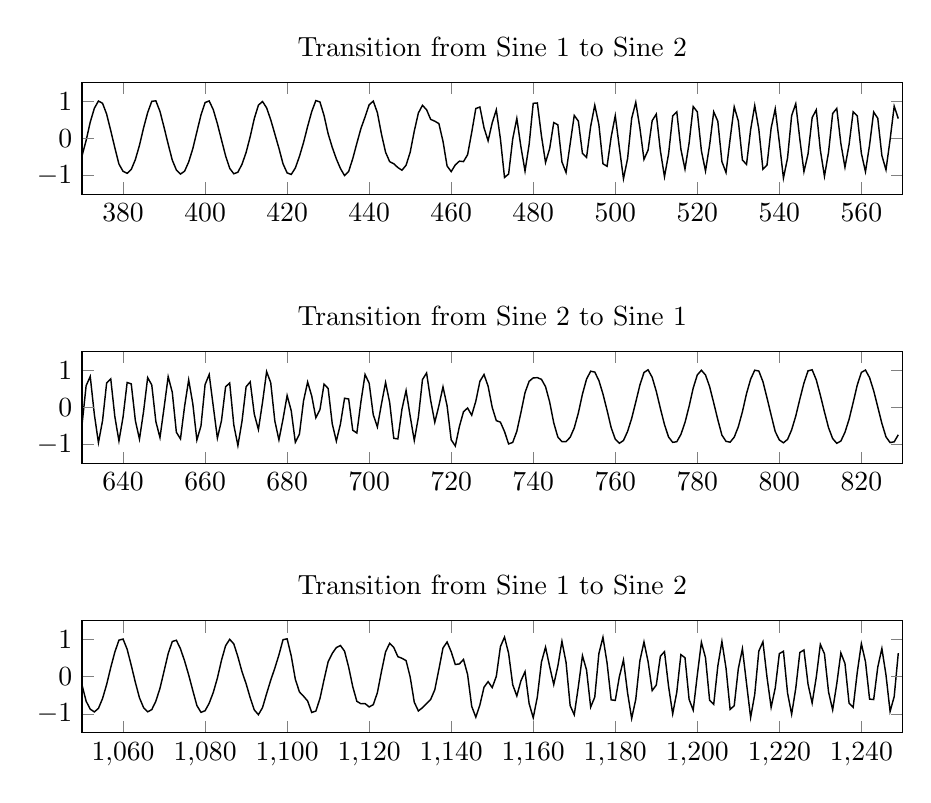
\begin{tikzpicture}

\begin{groupplot}[group style={group size=1 by 3,  vertical sep=2cm}]
\nextgroupplot[
title={Transition from Sine 1 to Sine 2},
xmin=370, xmax=570,
ymin=-1.5, ymax=1.5,
axis on top,
width=12cm,
height=3cm
]
\addplot [line width=0.52pt, black]
table {%
370 -0.469887136515006
371 -0.055900126111297
372 0.435392151045615
373 0.807178652138545
374 1.00238324994492
375 0.941774040969542
376 0.650609373066166
377 0.206318530622908
378 -0.253454569751855
379 -0.691672964092679
380 -0.886482471244131
381 -0.940053302945462
382 -0.834775690223924
383 -0.57073604553393
384 -0.187221290812036
385 0.279358321318127
386 0.691078708559456
387 0.994416536653014
388 1.00777945321689
389 0.723741173327175
390 0.293809031656939
391 -0.156077618771553
392 -0.58499137299469
393 -0.849982126887067
394 -0.959358068987078
395 -0.883377560134496
396 -0.63545886797481
397 -0.279621507985433
398 0.175279273651215
399 0.628009175501574
400 0.961129748141592
401 1.00455972872532
402 0.768346159791557
403 0.391950366168409
404 -0.0408982617684356
405 -0.469819979791096
406 -0.805409904269257
407 -0.952093386884826
408 -0.909402884113879
409 -0.69515025941976
410 -0.379477887637882
411 0.0463293783732923
412 0.533484302236957
413 0.890491417293258
414 0.989974320156623
415 0.818384716795066
416 0.500223836093564
417 0.119052051414151
418 -0.265613833896419
419 -0.684508065015056
420 -0.928151526047309
421 -0.970254824134137
422 -0.796755292593354
423 -0.486482517002647
424 -0.112954055904941
425 0.31974451468174
426 0.719689263922938
427 1.01386122201055
428 0.97840061915485
429 0.613195627323651
430 0.121999483665391
431 -0.241299240033879
432 -0.55188713224558
433 -0.811410366172426
434 -0.999977893362457
435 -0.889182935777263
436 -0.546125705490753
437 -0.132388323497478
438 0.266777351221604
439 0.573979828349156
440 0.901704530907799
441 0.99961624852908
442 0.691210781544212
443 0.113668879083947
444 -0.372402228502578
445 -0.626073814343427
446 -0.68296039985612
447 -0.784825402499675
448 -0.857072084741627
449 -0.722511208019971
450 -0.373601022309643
451 0.193843663285703
452 0.681622618536642
453 0.88694713996474
454 0.767439765598877
455 0.508999156467343
456 0.460661271933266
457 0.39559003540449
458 -0.0801935004731653
459 -0.742397078338094
460 -0.8936119250688
461 -0.713366785123559
462 -0.613027211330067
463 -0.624460430877025
464 -0.439328842887186
465 0.159506457347711
466 0.800092178501182
467 0.841633276165755
468 0.284480662020523
469 -0.0662865619827278
470 0.417935911394689
471 0.766213179923269
472 -0.0149791806671963
473 -1.05046081972996
474 -0.959040952487211
475 -0.016840007409145
476 0.535372593065978
477 -0.229045210288555
478 -0.879782839385083
479 -0.165334356727128
480 0.940414212109608
481 0.94983018923952
482 0.0687892252162227
483 -0.649356842680814
484 -0.279282661774165
485 0.422630228920985
486 0.363715154269071
487 -0.635182835031413
488 -0.918069163736079
489 -0.148904074210729
490 0.615125077256638
491 0.463511516379651
492 -0.405936968928556
493 -0.511179293225719
494 0.319991248312576
495 0.890057452631494
496 0.372407008725425
497 -0.68336450161112
498 -0.751298053817421
499 0.0373117158252971
500 0.608761687139569
501 -0.249963518051449
502 -1.08458437034854
503 -0.548250357618462
504 0.535990910206591
505 0.968162833566055
506 0.280261939928298
507 -0.565288794296428
508 -0.316211112297069
509 0.474089795816624
510 0.650325650129582
511 -0.332511470497966
512 -1.02987066677034
513 -0.416617741901936
514 0.600521635968389
515 0.712628958697929
516 -0.29452106763138
517 -0.826846803170813
518 -0.129538887736371
519 0.853143054376531
520 0.712059236285062
521 -0.334638104204599
522 -0.878600025769639
523 -0.18334744996548
524 0.712078093931176
525 0.459276486812627
526 -0.626465179248639
527 -0.91850612147029
528 -0.0170517009020086
529 0.845917440660807
530 0.466134539734589
531 -0.581524276043323
532 -0.701487511451976
533 0.232028537105629
534 0.882546200557154
535 0.244569487314278
536 -0.830869320710561
537 -0.714858002115824
538 0.276303755340472
539 0.793322940533297
540 -0.105968704955263
541 -1.0670159400296
542 -0.53099425565649
543 0.610607769521893
544 0.929260422138928
545 -0.0262371553917712
546 -0.893108926824292
547 -0.420024454963204
548 0.55535437626494
549 0.764725129567074
550 -0.317077328312123
551 -1.01789507293682
552 -0.369850431500416
553 0.667833701056743
554 0.803479240695866
555 -0.140504799109927
556 -0.777197942946835
557 -0.167694549389019
558 0.715084729589123
559 0.603188395032911
560 -0.404621827160139
561 -0.89638115229715
562 -0.176060974663842
563 0.705981991906594
564 0.537999048167268
565 -0.463817179233289
566 -0.846014674778095
567 -0.0365700080235721
568 0.861812817700026
569 0.529528603698274
};
\nextgroupplot[
title={Transition from Sine 2 to Sine 1},
xmin=630, xmax=830,
ymin=-1.5, ymax=1.5,
axis on top,
width=12cm,
height=3cm
]
\addplot [line width=0.52pt, black]
table {%
630 -0.457410263397318
631 0.585907724088303
632 0.83451643741434
633 -0.183255976078899
634 -0.945692641865413
635 -0.354051288374978
636 0.658552601103541
637 0.769527990606456
638 -0.247998793016675
639 -0.897162777722184
640 -0.257077342321989
641 0.671385833038383
642 0.634259362207398
643 -0.353108141567373
644 -0.849172191433555
645 -0.109210366876644
646 0.802746029655274
647 0.605820118333213
648 -0.377972562499866
649 -0.80851845966774
650 -0.00705365326177588
651 0.828898115951881
652 0.409335511555204
653 -0.665357026077952
654 -0.843265242424194
655 0.029151430926386
656 0.743948276862174
657 0.104943510779022
658 -0.873697729695745
659 -0.494047720824597
660 0.616340829173539
661 0.885844889084615
662 0.0287610637476635
663 -0.821886411928209
664 -0.351548041381859
665 0.556744582226322
666 0.657753440673497
667 -0.467768361579448
668 -1.02397840146392
669 -0.36914976713007
670 0.557631657345698
671 0.68845681304979
672 -0.182122792814322
673 -0.590976313286865
674 0.137319079604784
675 0.962787125984563
676 0.667790813549115
677 -0.35873836510248
678 -0.869497096462623
679 -0.311265895625012
680 0.322425578770857
681 -0.0860939148610888
682 -0.933156984033587
683 -0.713799082923339
684 0.177081825877302
685 0.684236308034705
686 0.308237910583137
687 -0.274484125099231
688 -0.0600012518793218
689 0.626908452451911
690 0.51226837531718
691 -0.437134773002947
692 -0.902446550572733
693 -0.442042619899997
694 0.24791725254028
695 0.229159939272588
696 -0.610938617534598
697 -0.685745810358698
698 0.157750241573195
699 0.88706697638182
700 0.651824019287483
701 -0.195596094962452
702 -0.523408710492398
703 0.0947800992587583
704 0.671616443951664
705 0.13532569152234
706 -0.82818257397586
707 -0.843819039501354
708 -0.0427750805607606
709 0.456704627746278
710 -0.233939682508981
711 -0.886103387852109
712 -0.262562803674579
713 0.750453447089765
714 0.927373724210627
715 0.188744783148404
716 -0.398005371618242
717 0.0487466059012583
718 0.554285790721576
719 0.0442603337380392
720 -0.867955412141625
721 -1.03472228357065
722 -0.50932991962683
723 -0.113330052652509
724 -0.0138950768041038
725 -0.206892034560886
726 0.167942906711807
727 0.704587541625081
728 0.886225713353533
729 0.572868003098231
730 0.00352780858666858
731 -0.353021320246991
732 -0.393876862395707
733 -0.645997953831139
734 -0.978452513538061
735 -0.937733063588112
736 -0.638997804390021
737 -0.135924168240005
738 0.399376021804846
739 0.703696753830441
740 0.794796822065712
741 0.80171657820455
742 0.757242515422755
743 0.560323219576543
744 0.150894906317543
745 -0.411348906915489
746 -0.79382783462788
747 -0.917212885370977
748 -0.915842446928794
749 -0.800203912742535
750 -0.549726435973358
751 -0.147802603314151
752 0.359570128024487
753 0.763433440808639
754 0.974788787188453
755 0.952165249457553
756 0.726525157887872
757 0.363554745391714
758 -0.0742820546183571
759 -0.541568956496751
760 -0.850749482049846
761 -0.961587427456541
762 -0.886427400353561
763 -0.642956684977205
764 -0.294140788576811
765 0.147143414057719
766 0.600706701961427
767 0.93998543638939
768 1.01256987622359
769 0.809421455942977
770 0.433585345594794
771 -0.0241508864247589
772 -0.460691306451605
773 -0.794161277381386
774 -0.936177046970388
775 -0.919016570780043
776 -0.724478915761702
777 -0.402410256835773
778 0.030342159626789
779 0.521911248809922
780 0.874985473545231
781 1.00084902066763
782 0.872850557881147
783 0.563463704328907
784 0.124556509757358
785 -0.327536609768321
786 -0.74238964095439
787 -0.908960572365996
788 -0.930995443649662
789 -0.797525699419429
790 -0.516969978567734
791 -0.1129629963715
792 0.373570752124373
793 0.760285034558531
794 1.00218271778742
795 0.979761777960214
796 0.694374608155557
797 0.25597990542548
798 -0.202305001609502
799 -0.646230337582222
800 -0.871938285258025
801 -0.94823435087726
802 -0.857042064075629
803 -0.600010552328369
804 -0.231215519904011
805 0.226551141710406
806 0.657871792839221
807 0.984626796387867
808 1.01281878411036
809 0.744451342365809
810 0.329010330491753
811 -0.118498932707272
812 -0.5436005465926
813 -0.834458223778044
814 -0.961910669597993
815 -0.901318416144772
816 -0.665420230262308
817 -0.318330888997502
818 0.134213030125262
819 0.605036740588301
820 0.942827982153054
821 1.00510437963079
822 0.801430962781817
823 0.449891927681617
824 0.014446385493583
825 -0.426646905809111
826 -0.789856301486724
827 -0.942185547569239
828 -0.921949410581253
829 -0.733250308770486
};
\nextgroupplot[
title={Transition from Sine 1 to Sine 2},
xmin=1050, xmax=1250,
ymin=-1.5, ymax=1.5,
axis on top,
width=12cm,
height=3cm
]
\addplot [line width=0.52pt, black]
table {%
1050 -0.224347939442927
1051 -0.659342308519419
1052 -0.873507716741155
1053 -0.947349285295172
1054 -0.851612275746619
1055 -0.587304244678871
1056 -0.210314220781092
1057 0.246166792783724
1058 0.660767890535504
1059 0.98048721753229
1060 1.01058294391939
1061 0.735303319403764
1062 0.303076437286959
1063 -0.151791228093023
1064 -0.567587519983102
1065 -0.830421533082797
1066 -0.944700937659204
1067 -0.885806588501324
1068 -0.657442947992333
1069 -0.313183008222317
1070 0.148859817125284
1071 0.619002029635064
1072 0.943929338923521
1073 0.977463699842311
1074 0.748514536889445
1075 0.423035941585966
1076 0.0476563736189198
1077 -0.370290777516534
1078 -0.774984585294598
1079 -0.958128642104967
1080 -0.915465711476532
1081 -0.712425202627135
1082 -0.423147465039793
1083 -0.036471637380023
1084 0.441125086512591
1085 0.830579611480725
1086 1.00301990792371
1087 0.880213916864111
1088 0.533959705015882
1089 0.132420196266485
1090 -0.189868724179731
1091 -0.567135030605418
1092 -0.894519284849107
1093 -1.02118533928507
1094 -0.831847440131194
1095 -0.456194263476222
1096 -0.095747968911982
1097 0.228581544211104
1098 0.583817888829003
1099 0.993184437749212
1100 1.01625291841702
1101 0.558621643816002
1102 -0.0694179651283972
1103 -0.409195716316065
1104 -0.525481314507107
1105 -0.653702273828313
1106 -0.962205678192988
1107 -0.92501497135482
1108 -0.589744187419099
1109 -0.0817998910839236
1110 0.400474422999606
1111 0.624534651154836
1112 0.78108521823973
1113 0.837524967095422
1114 0.684501876311464
1115 0.257457577370929
1116 -0.269073966672484
1117 -0.662256665082389
1118 -0.727923569638187
1119 -0.723334098497563
1120 -0.813201646061374
1121 -0.752808845395173
1122 -0.432848349328547
1123 0.137661356625569
1124 0.666072203615698
1125 0.894881635191695
1126 0.785791938729416
1127 0.537639623479459
1128 0.49360403623442
1129 0.431494895609193
1130 -0.00861298830773538
1131 -0.686649653965726
1132 -0.920976547718235
1133 -0.8330409272195
1134 -0.721151385659448
1135 -0.609193563399765
1136 -0.353444433498771
1137 0.196145069896714
1138 0.770925866783996
1139 0.930771600188509
1140 0.669486460445155
1141 0.326425419947196
1142 0.342492005105519
1143 0.461988261183749
1144 0.0580204285262646
1145 -0.796753525064276
1146 -1.08696739737932
1147 -0.757618370349529
1148 -0.283768497752127
1149 -0.134662368325581
1150 -0.293993215607798
1151 0.00840239388696113
1152 0.806337806433094
1153 1.06224649514453
1154 0.624091387351963
1155 -0.217184989688458
1156 -0.518607483175264
1157 -0.11207178140753
1158 0.133248531271261
1159 -0.724152385736208
1160 -1.10304299466842
1161 -0.547899842127531
1162 0.389682200134291
1163 0.79197631263939
1164 0.274923126582309
1165 -0.210797471556706
1166 0.28282770613123
1167 0.94899987274146
1168 0.383449803237797
1169 -0.774508573936511
1170 -1.0244097452523
1171 -0.268085479278904
1172 0.562963518870526
1173 0.177676062454932
1174 -0.818234887823617
1175 -0.549759166954618
1176 0.618020584997705
1177 1.05834900387743
1178 0.369373648383696
1179 -0.62243174178325
1180 -0.638451167053079
1181 0.000247256346655308
1182 0.447152687407212
1183 -0.434126690914113
1184 -1.1223087972784
1185 -0.607316636755916
1186 0.425945750359711
1187 0.932673944335444
1188 0.404133031378011
1189 -0.374245493212239
1190 -0.227229269251263
1191 0.548965964890666
1192 0.671555563515891
1193 -0.264658410534093
1194 -1.00026762591993
1195 -0.415293712004664
1196 0.59166629632144
1197 0.508960903035358
1198 -0.610474620816413
1199 -0.900047833531108
1200 0.0424270317277314
1201 0.924635296389947
1202 0.508583127054875
1203 -0.632879222292831
1204 -0.743484511448957
1205 0.280439724436218
1206 0.945100690190164
1207 0.230196509086494
1208 -0.879617747204655
1209 -0.781767771567955
1210 0.212147385039286
1211 0.750723605698127
1212 -0.181142089018346
1213 -1.09722476010589
1214 -0.475806043640971
1215 0.687797648096819
1216 0.936623519115382
1217 -0.0214113202366981
1218 -0.824432282995716
1219 -0.304950103208181
1220 0.618015921630753
1221 0.682602110332863
1222 -0.43722212975974
1223 -1.00877087123278
1224 -0.316742992785232
1225 0.648973693091121
1226 0.716639828505353
1227 -0.203850020178813
1228 -0.70820412118076
1229 -0.0175758799301426
1230 0.866554171901477
1231 0.612733576648143
1232 -0.412821577854985
1233 -0.892688869605219
1234 -0.195000969047729
1235 0.637554822175676
1236 0.354034802532995
1237 -0.710823054184549
1238 -0.82390494235532
1239 0.11866059104442
1240 0.885477953670592
1241 0.401726524852983
1242 -0.602203128801395
1243 -0.614389496125281
1244 0.25810621279342
1245 0.756129260332788
1246 0.0454548206608226
1247 -0.934467964200425
1248 -0.536577676934316
1249 0.631291968477322
};
\end{groupplot}

\end{tikzpicture}

      	\caption[Output of the HRFC in the binocular rivalry condition]{Output around transition points of hypotheses of the hierarchical random feature conceptors top level in the binocular rivalry condition. The switch in the generated signal can be observed clearly, as well as the production of a combination of both prototype patterns at the immediate point of transition. }
        \label{predictions}
    \end{figure}

    
	Figure \ref{predictions} shows the output of the top level module around transition points of hypotheses. This signal is the systems prediction of the input pattern. The plot shows how the predictions changes under the change of the leading hypothesis. Closely around the transition point the produced signal are slightly unstable, reflecting that the hypotheses are equally likely at these points in time. At the transition points the conceptor that controls the system is the disjunction of both patterns and the resulting prediction a combination of both patterns. One can observe this fact for example in the topmost plot between timestep 460 and 475. The peak has the overall width of the fist sinewave, but at the same time two more peaks of the period of the second sinewave 'on top'.
	
    \begin{figure}
           	\centering
       	    % This file was created by matplotlib2tikz v0.5.4.
% The lastest updates can be retrieved from
% 
% https://github.com/nschloe/matplotlib2tikz
% 
% where you can also submit bug reports and leavecomments.
% 
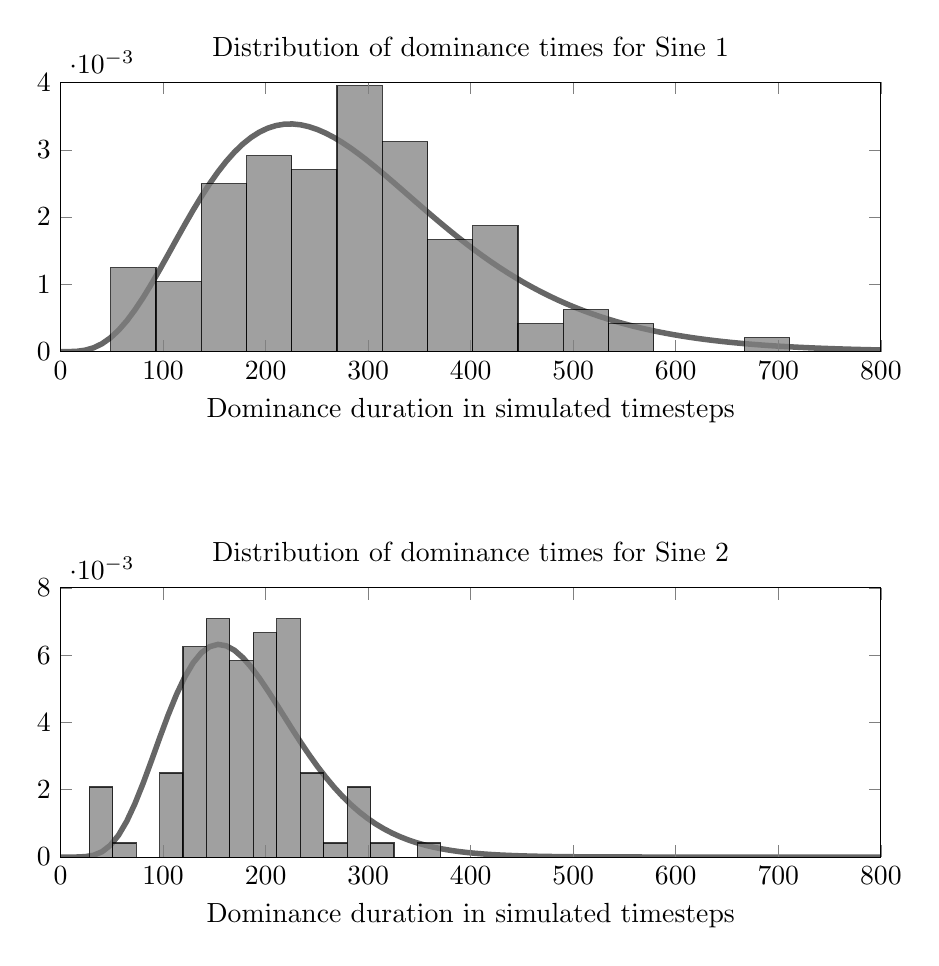
\begin{tikzpicture}

%draw[draw=white,fill=lightgray] (axis cs:0,0) rectangle (axis cs:1,1);
\begin{groupplot}[group style={group size=1 by 2,  vertical sep=3cm}]
\nextgroupplot[
title={Distribution of dominance times for Sine 1},
xlabel={Dominance duration in simulated timesteps},
xmin=0, xmax=800,
ymin=0, ymax=0.004,
axis on top,
width=12cm,
height=5cm
]
\addplot [domain=0:800,line width=2.0pt, black, opacity=0.6]
table {%
0 0
8.08080808080808 4.69780351705954e-07
16.1616161616162 5.5856266058629e-06
24.2424242424242 2.24640410305493e-05
32.3232323232323 5.79648178613469e-05
40.4040404040404 0.000117281807944635
48.4848484848485 0.000203467937640104
56.5656565656566 0.000317440748551388
64.6464646464647 0.00045823483263232
72.7272727272727 0.000623365861557552
80.8080808080808 0.000809225946970934
88.8888888888889 0.00101146365155336
96.969696969697 0.00122532319429696
105.050505050505 0.00144593091520422
113.131313131313 0.00166852558273843
121.212121212121 0.00188863432702668
129.292929292929 0.00210219896630683
137.373737373737 0.00230565900649982
145.454545454545 0.00249599814268944
153.535353535354 0.00267076102732503
161.616161616162 0.00282804663481838
169.69696969697 0.00296648391138065
177.777777777778 0.00308519466420564
185.858585858586 0.00318374788922902
193.939393939394 0.00326210900863399
202.020202020202 0.0033205868161788
210.10101010101 0.00335978032538326
218.181818181818 0.00338052718883115
226.262626262626 0.00338385490661686
234.343434343434 0.00337093566481556
242.424242424242 0.00334304533506653
250.505050505051 0.00330152691702433
258.585858585859 0.00324775850919185
266.666666666667 0.00318312574317973
274.747474747475 0.00310899850475952
282.828282828283 0.00302671168575449
290.909090909091 0.00293754965803624
298.989898989899 0.00284273412953688
307.070707070707 0.00274341502778505
315.151515151515 0.00264066405521013
323.232323232323 0.00253547056910478
331.313131313131 0.00242873945500498
339.393939393939 0.00232129068312816
347.474747474748 0.00221386026161493
355.555555555556 0.00210710232622148
363.636363636364 0.00200159213269099
371.717171717172 0.00189782974443782
379.79797979798 0.00179624423377112
387.878787878788 0.00169719823920622
395.959595959596 0.00160099274415238
404.040404040404 0.00150787196322934
412.121212121212 0.00141802824155258
420.20202020202 0.00133160688950771
428.282828282828 0.00124871089083558
436.363636363636 0.00116940543533587
444.444444444444 0.00109372223926357
452.525252525253 0.00102166362665399
460.606060606061 0.000953206353492512
468.686868686869 0.000888305163976777
476.767676767677 0.0008268960742332
484.848484848485 0.000768899383876851
492.929292929293 0.000714222419867898
501.010101010101 0.000662762020337754
509.090909090909 0.000614406768543521
517.171717171717 0.000569038988962135
525.252525252525 0.00052653651884843
533.333333333333 0.00048677426943792
541.414141414141 0.000449625591450585
549.49494949495 0.000414963459712956
557.575757575758 0.0003826614916212
565.656565656566 0.000352594813868899
573.737373737374 0.000324640791404589
581.818181818182 0.00029867963200402
589.89898989899 0.000274594879173273
597.979797979798 0.000252273805368992
606.060606060606 0.000231607716754094
614.141414141414 0.000212492179920565
622.222222222222 0.000194827180221017
630.30303030303 0.000178517220569977
638.383838383838 0.000163471368814518
646.464646464647 0.000149603261039312
654.545454545455 0.000136831067469292
662.626262626263 0.000125077426967873
670.707070707071 0.000114269355502843
678.787878787879 0.000104338133367149
686.868686868687 9.52191753984771e-05
694.949494949495 8.68518879396465e-05
703.030303030303 7.91795158207634e-05
711.111111111111 7.21489822224486e-05
719.191919191919 6.57107238959244e-05
727.272727272727 5.98185238683557e-05
735.353535353535 5.44293434486965e-05
743.434343434344 4.95031550682621e-05
751.515151515152 4.50027772391933e-05
759.59595959596 4.08937126907112e-05
767.676767676768 3.7143990545465e-05
775.757575757576 3.37240132242154e-05
783.838383838384 3.06064086145824e-05
791.919191919192 2.77658879066444e-05
800 2.5179109382995e-05
};
\draw[draw=black,fill=white!50.196078431372548!black,opacity=0.75] (axis cs:49,0) rectangle (axis cs:93.1333333333333,0.00124726295074697);
\draw[draw=black,fill=white!50.196078431372548!black,opacity=0.75] (axis cs:93.1333333333333,0) rectangle (axis cs:137.266666666667,0.00103938579228914);
\draw[draw=black,fill=white!50.196078431372548!black,opacity=0.75] (axis cs:137.266666666667,0) rectangle (axis cs:181.4,0.00249452590149394);
\draw[draw=black,fill=white!50.196078431372548!black,opacity=0.75] (axis cs:181.4,0) rectangle (axis cs:225.533333333333,0.0029102802184096);
\draw[draw=black,fill=white!50.196078431372548!black,opacity=0.75] (axis cs:225.533333333333,0) rectangle (axis cs:269.666666666667,0.00270240305995177);
\draw[draw=black,fill=white!50.196078431372548!black,opacity=0.75] (axis cs:269.666666666667,0) rectangle (axis cs:313.8,0.00394966601069874);
\draw[draw=black,fill=white!50.196078431372548!black,opacity=0.75] (axis cs:313.8,0) rectangle (axis cs:357.933333333333,0.00311815737686743);
\draw[draw=black,fill=white!50.196078431372548!black,opacity=0.75] (axis cs:357.933333333333,0) rectangle (axis cs:402.066666666667,0.00166301726766263);
\draw[draw=black,fill=white!50.196078431372548!black,opacity=0.75] (axis cs:402.066666666667,0) rectangle (axis cs:446.2,0.00187089442612046);
\draw[draw=black,fill=white!50.196078431372548!black,opacity=0.75] (axis cs:446.2,0) rectangle (axis cs:490.333333333333,0.000415754316915657);
\draw[draw=black,fill=white!50.196078431372548!black,opacity=0.75] (axis cs:490.333333333333,0) rectangle (axis cs:534.466666666667,0.000623631475373485);
\draw[draw=black,fill=white!50.196078431372548!black,opacity=0.75] (axis cs:534.466666666667,0) rectangle (axis cs:578.6,0.000415754316915657);
\draw[draw=black,fill=white!50.196078431372548!black,opacity=0.75] (axis cs:578.6,0) rectangle (axis cs:622.733333333333,0);
\draw[draw=black,fill=white!50.196078431372548!black,opacity=0.75] (axis cs:622.733333333333,0) rectangle (axis cs:666.866666666667,0);
\draw[draw=black,fill=white!50.196078431372548!black,opacity=0.75] (axis cs:666.866666666667,0) rectangle (axis cs:711,0.000207877158457829);
%\draw[fill=white,draw opacity=0] (axis cs:0,0) rectangle (axis cs:1,1);
\nextgroupplot[
title={Distribution of dominance times for Sine 2},
xlabel={Dominance duration in simulated timesteps},
xmin=0, xmax=800,
ymin=0, ymax=0.008,
axis on top,
width=12cm,
height=5cm]
\addplot [domain=0:800,line width=2.0pt, black, opacity=0.6]
table {%
0 0
8.08080808080808 2.85566830090683e-08
16.1616161616162 1.46667290829751e-06
24.2424242424242 1.28526045349379e-05
32.3232323232323 5.46043279061185e-05
40.4040404040404 0.000156018941900639
48.4848484848485 0.000346859207597452
56.5656565656566 0.000648525321137459
64.6464646464647 0.00106821195850183
72.7272727272727 0.00159715724551185
80.8080808080808 0.00221246283712305
88.8888888888889 0.00288120997459992
96.969696969697 0.0035654977825332
105.050505050505 0.00422729504664813
113.131313131313 0.00483239211770421
121.212121212121 0.0053531203386781
129.292929292929 0.00576980256114858
137.373737373737 0.0060710909485311
145.454545454545 0.0062534470857769
153.535353535354 0.00632004655751623
161.616161616162 0.00627937001301372
169.69696969697 0.00614369663297983
177.777777777778 0.00592766001612661
185.858585858586 0.00564697163551186
193.939393939394 0.00531736942886329
202.020202020202 0.00495381157994602
210.10101010101 0.00456990856917577
218.181818181818 0.00417756915939578
226.262626262626 0.00378682647235444
234.343434343434 0.00340580682285345
242.424242424242 0.0030408047180172
250.505050505051 0.00269643085573023
258.585858585859 0.00237580484063664
266.666666666667 0.00208076976680091
274.747474747475 0.00181211116580744
282.828282828283 0.0015697676950627
290.909090909091 0.00135302513221053
298.989898989899 0.00116068866847506
307.070707070707 0.000991231166133993
315.151515151515 0.000842917027941053
323.232323232323 0.000713902713146827
331.313131313131 0.000602315830693284
339.393939393939 0.000506315248721694
347.474747474748 0.000424134875499797
355.555555555556 0.000354113772317122
363.636363636364 0.000294715121781966
371.717171717172 0.0002445363493382
379.79797979798 0.000202312423040797
387.878787878788 0.000166914066989891
395.959595959596 0.000137342338464104
404.040404040404 0.000112720751525813
412.121212121212 9.22858888527032e-05
420.20202020202 7.53772327414241e-05
428.282828282828 6.14267666017566e-05
436.363636363636 4.99487487670384e-05
444.444444444444 4.05299387783167e-05
452.525252525253 3.28204594462777e-05
460.606060606061 2.65254026561824e-05
468.686868686869 2.13972297474395e-05
476.767676767677 1.72289752360027e-05
484.848484848485 1.38482328028458e-05
492.929292929293 1.11118823317414e-05
501.010101010101 8.90150418573384e-06
509.090909090909 7.11942005129191e-06
517.171717171717 5.68529706085782e-06
525.252525252525 4.53325232506445e-06
533.333333333333 3.60939751284457e-06
541.414141414141 2.86976697193157e-06
549.49494949495 2.27857752252064e-06
557.575757575758 1.80677306703651e-06
565.656565656566 1.43081223951219e-06
573.737373737374 1.13166226136168e-06
581.818181818182 8.93966839723676e-07
589.89898989899 7.05360257333919e-07
597.979797979798 5.55903716242862e-07
606.060606060606 4.37623497621275e-07
614.141414141414 3.44133592441111e-07
622.222222222222 2.70328162375993e-07
630.30303030303 2.12131534483663e-07
638.383838383838 1.66295449253591e-07
646.464646464647 1.30235003350886e-07
654.545454545455 1.01896189673218e-07
662.626262626263 7.96491705923693e-08
670.707070707071 6.22024557355334e-08
678.787878787879 4.85340210157828e-08
686.868686868687 3.78361256786986e-08
694.949494949495 2.94711808975785e-08
703.030303030303 2.29365161996995e-08
711.111111111111 1.78362954634079e-08
719.191919191919 1.38591667748388e-08
727.272727272727 1.07605023553097e-08
735.353535353535 8.34830648278649e-09
743.434343434344 6.47204961646696e-09
751.515151515152 5.01383315866938e-09
759.59595959596 3.88140760063227e-09
767.676767676768 3.00266230663982e-09
775.757575757576 2.32128212094472e-09
783.838383838384 1.79332781868081e-09
791.919191919192 1.38454702761083e-09
800 1.06826196563467e-09
};
\draw[draw=black,fill=white!50.196078431372548!black,opacity=0.75] (axis cs:28,0) rectangle (axis cs:50.8666666666667,0.00208246563931695);
\draw[draw=black,fill=white!50.196078431372548!black,opacity=0.75] (axis cs:50.8666666666667,0) rectangle (axis cs:73.7333333333333,0.00041649312786339);
\draw[draw=black,fill=white!50.196078431372548!black,opacity=0.75] (axis cs:73.7333333333333,0) rectangle (axis cs:96.6,0);
\draw[draw=black,fill=white!50.196078431372548!black,opacity=0.75] (axis cs:96.6,0) rectangle (axis cs:119.466666666667,0.00249895876718034);
\draw[draw=black,fill=white!50.196078431372548!black,opacity=0.75] (axis cs:119.466666666667,0) rectangle (axis cs:142.333333333333,0.00624739691795085);
\draw[draw=black,fill=white!50.196078431372548!black,opacity=0.75] (axis cs:142.333333333333,0) rectangle (axis cs:165.2,0.00708038317367764);
\draw[draw=black,fill=white!50.196078431372548!black,opacity=0.75] (axis cs:165.2,0) rectangle (axis cs:188.066666666667,0.00583090379008746);
\draw[draw=black,fill=white!50.196078431372548!black,opacity=0.75] (axis cs:188.066666666667,0) rectangle (axis cs:210.933333333333,0.00666389004581424);
\draw[draw=black,fill=white!50.196078431372548!black,opacity=0.75] (axis cs:210.933333333333,0) rectangle (axis cs:233.8,0.00708038317367763);
\draw[draw=black,fill=white!50.196078431372548!black,opacity=0.75] (axis cs:233.8,0) rectangle (axis cs:256.666666666667,0.00249895876718034);
\draw[draw=black,fill=white!50.196078431372548!black,opacity=0.75] (axis cs:256.666666666667,0) rectangle (axis cs:279.533333333333,0.000416493127863391);
\draw[draw=black,fill=white!50.196078431372548!black,opacity=0.75] (axis cs:279.533333333333,0) rectangle (axis cs:302.4,0.00208246563931695);
\draw[draw=black,fill=white!50.196078431372548!black,opacity=0.75] (axis cs:302.4,0) rectangle (axis cs:325.266666666667,0.00041649312786339);
\draw[draw=black,fill=white!50.196078431372548!black,opacity=0.75] (axis cs:325.266666666667,0) rectangle (axis cs:348.133333333333,0);
\draw[draw=black,fill=white!50.196078431372548!black,opacity=0.75] (axis cs:348.133333333333,0) rectangle (axis cs:371,0.00041649312786339);
%\draw[fill=white,draw opacity=0] (axis cs:0,0) rectangle (axis cs:1,1);
\end{groupplot}

\end{tikzpicture}
      	\caption[Distrubution of dominance times]{Distrubution of dominance times, seperately for each sinewave. Both histograms were fit to a gamma distribution function. The distribution of dominance times in the binocular rivalry simulation is similar to data acquired from experiments in humans, when they were viewing rivalling stimuli.}
       	\label{dominance_times}
    \end{figure}
    
    We calculated the distribution of dominance times on the data of the third level hypothesis vector. We in particular calculated the dominance times for each sinewave separately, in order not to get a mixed distribution that is skewed to either side because the patterns have a different signal strength. Both distributions are plotted in Figure \ref{dominance_times}. The distributions show similarity to the results of \cite{Levelt1965}. As Levelt did, we fit gamma functions to the data. For the general form 
    
    
    \begin{equation}
{\frac {\beta ^{\alpha }}{\Gamma (\alpha )}}x^{\alpha \,-\,1}e^{-\beta x}
    \end{equation}
    
    We estimated the parameters $\alpha$ and $\beta$ using the \texttt{scipy.gamma} package for Python:



	\begin{center}
    \begin{tabular}{ r|c|c| }
    \multicolumn{1}{r}{}
     &  \multicolumn{1}{c}{$\alpha$}
     & \multicolumn{1}{c}{$\beta$} \\
    \cline{2-3}
    sine 1 & 4.77 & 0.01684 \\
    \cline{2-3}
    sine 2 & 7.15 & 0.03982 \\
    \cline{2-3}
    \end{tabular}
    \end{center}

    \vspace{1cm}
    These yield the following equation of the fit for sine 1
     
     \begin{equation}
		{\frac {0.01684 ^{4.77}}{\Gamma (4.77)}}x^{4.77 \,-\,1}e^{-0.01684 x}
     \end{equation}
     and sine 2 respectively
     
     \begin{equation}
		{\frac {0.03982 ^{7.15}}{\Gamma (7.15)}}x^{7.15 \,-\,1}e^{-0.03982 x}     
     \end{equation}
     $\Gamma (t)$ refers to the gamma function.
     \begin{equation}
      \Gamma (t)=\int _{0}^{\infty }x^{t-1}e^{-x}\,dx.
     \end{equation}
     It extends factorials to all complex numbers except negative integers.

\section{Discussion}

    We used a recent artificial neural network model, based on the paradigm of reservoir computing, to instantiate a simulation of the binocular rivalry in terms of predictive coding. This was a promising endeavour to us, since besides long standing efforts in the area of binocular rivalry, many open questions remain. In particular, we hope that we were able to deliver a first step into the direction of a model that is based on a general framework for perception.
    
    The need for such a model was recently brought up from within the binocular rivarly research community in \cite{Hohwy2008}. We emphasise however that our model is barely a first step into a promising direction. Even more so, we clearly point out that we can not make any full blown claims about the architecture actually working according to the ideas in the predictive coding framework. In the following we will detail our doubts. 
    We have the intuition that coming short of real results in these points is not due to the fact that the direction of research leads nowhere. Quite the opposite, we think that waterproof results are coming up further along the way. We realise that we have only made the first steps in the direction of using the conceptor architecture for cognitive modelling tasks and we are sure that there is a lot to learn about these systems. Especially as the field of related mathematical research is very young, our study will greatly profit from upcoming results in that area.
  
    
    \subsection{Bayesian perceptual inference}
    In how far does our model perform Bayesian perceptual inference? Under the predictive coding theory the brain generates and tests hypothesis about the causes of the sensory data it encounters. In our simulation the system has learned two prototype patterns. These two patterns are "the world" for the system. Besides the driving input itself, its internal representation of the prototype patterns is the only information it has access to during runtime. As the system is also not adapting or learning any new patterns during the course of the binocular rivalry simulation, the only hypothesis it can make up involve the two prototype patterns.
    The simulation of the binocular rivalry condition shows that the system adapts its hypothesis about the current input in accordance to the input. On the level of the hypotheses it shows an alternating behaviour, just as it is the key observation in the binocular rivalry condition in humans. Insofar we have a working example of a challenging situation for a perceptual system. This of course is not sufficient to proof that the system is actually doing Bayesian perceptual inference. We believe a valid starting point to investigate whether a system is instantiating an inference mechanism of the kind that is inherent in humans, is to work with a system that has \textit{no} clear issues that suggest it is \textit{not} employing such a mechanism. In order to rigorously identify dynamics of the system with parts of the Bayesian theorem more work in that direction needs to be done. We had to leave this very interesting point to future investigations.  
    
	\subsection{Low prior for compound hypothesis}
 	As in the preceding paragraph discussed, the system has only the option to make up hypotheses from the two prototype pattern it knows. It can, however, settle on a mixture of these, maintaining for example the hypothesis that a mixture of the prototype patterns causes the current sensory input. This is in fact the case, if the system is run without the effect of the feedback loop. In many situations this is highly desirable and it is a research project in its own right in how far conceptor combinations really are able to combine concepts. Nevertheless in the special case of humans viewing binocular rivalry stimuli, the hypothesis of a mixture of both stimuli is a priori highly unlikely. Face-house compounds for example do usually not appear in the world. We tried to reflect this low prior probability for the compound hypothesis within a conceptor, but we were not able to construct it. This was mostly due to the notion of the negation of a conceptor. A conceptor is representing an ellipsoid in the networks state space, and its negation is defined by  \cite{Jaeger2014}  as and ellipsoid spanned by the orthogonal directions of the original conceptor. A negative conceptor is not the complete state space which is not occupied by the original conceptor, as one might be tempted to think. This reasoning let us believe that we would not be able to build the low prior for the compound hypothesis into a conceptor. In the end we circumvented this issue by the construction of the feedback loop. The signal corresponding to the winning\footnote{The winning hypothesis, as explained in the preceding section, is the hypothesis that is assigned the larger probability, even if it is only in slight advance.  } hypothesis is completely subtracted from the input signal. Therefore the actual input to the system always corresponds only to one signal plus the added noise. This design choice can be supported by the argument of a strong effect of the prediction of the system on the actual perception. The reasoning is that the predicted signal is completely explained and therefore can be subtracted from the input signal. We employed this mechanisms, however, it was not the original approach. In the original approach we tried to take the bare prediction of the system on the top layer and subtract that from the input. This turned out to be not suitable for our attempt, as reservoir systems as we use them produce inevitable phase shifts of the generated signal versus the input signal. Moreover we were stuck with the just mentioned problem of the system believing that the current input is a mix of both signals. We therefore construct the input signal on the basis of the hypothesis vector only, and not with the influence of direct feedback from the top layer prediction of the system.  
      
    \subsection{Prediction error minimization}
    The hierarchical random feature architecture tries to minimize prediction error by selecting the best hypothesis in order to predict the incoming sensory data. The residuum of the incoming data which can not be explained is called the prediction error. In contrast to predictive coding the proposed architecture does not signal the prediction error upwards in the hierarchy, but a denoised version of the  sensory input. 'Denoised' means in this context that parts of the signal which are not predictable under the current hypothesis are regarded as noise and are suppressed. This in fact leads to less prediction error on higher layers of the hierarchy, as the prediction error is suppressed by each layer. This mechanism is therefore actually minimizing prediction error, but in a slightly different fashion than the usually in predictive coding proposed upwards signalling of the residual signals or prediction errors. Minimizing prediction error just by suppressing all signals that can not be predicted on its own does not seem very useful. But this process is aided by a general assessment of fit of all prototype patterns to the input signal. This is inherent in the conceptor mechanism. Therefore the mechanism for prediction error minimization is different in the hierarchical random feature conceptor as compared to the usual notion in predictive coding. This issue is still in debate, also for the predictive coding research community, as we are not aware of any clear cut evidence in favour of and against other possible realisations of error signalling. 
    
    %\paragraph{Second order inference / trust variables}
    
    \subsection{Comparing dominance times to Levelt's work}
    The distribution of dominance times that we obtained from the simulation is of the same form as the dominance time distribution of Levelt's work in the 60s. We are not sure why our architecture changes its perception with these statistical regularities. The shape of the dominance times histogram might even be due to the nature of the noise that is added to the stimulus.
    The similarity, by itself, is a success for us. We set out to this endeavour without knowing if we would find encouraging results on the way. It makes us curious that the distribution of dominance times is so similar between our, not parametrically optimised setup, and data from the real world. Still, we can not draw any claims from the observation at this point. Rather, we are at a point where plenty of directions of future research are on offer.





\section*{Disclosure/Conflict-of-Interest Statement}
%Frontiers follows the recommendations by the International Committee of Medical Journal Editors (http://www.icmje.org/ethical_4conflicts.html) which require that all financial, commercial or other relationships that might be perceived by the academic community as representing a potential conflict of interest must be disclosed. If no such relationship exists, authors will be asked to declare that the research was conducted in the absence of any commercial or financial relationships that could be construed as a potential conflict of interest. When disclosing the potential conflict of interest, the authors need to address the following points:
%•	Did you or your institution at any time receive payment or services from a third party for any aspect of the submitted work?
%•	Please declare financial relationships with entities that could be perceived to influence, or that give the appearance of potentially influencing, what you wrote in the submitted work.
%•	Please declare patents and copyrights, whether pending, issued, licensed and/or receiving royalties relevant to the work.
%•	Please state other relationships or activities that readers could perceive to have influenced, or that give the appearance of potentially influencing, what you wrote in the submitted work.

The authors declare that the research was conducted in the absence of any commercial or financial relationships that could be construed as a potential conflict of interest.

\section*{Author Contributions}
%When determining authorship the following criteria should be observed:
%•	Substantial contributions to the conception or design of the work; or the acquisition, analysis, or interpretation of data for the work; AND
%•	Drafting the work or revising it critically for important intellectual content; AND
%•	Final approval of the version to be published ; AND
%•	Agreement to be accountable for all aspects of the work in ensuring that questions related to the accuracy or integrity of any part of the work are appropriately investigated and resolved.
%Contributors who meet fewer than all 4 of the above criteria for authorship should not be listed as authors, but they should be acknowledged. (http://www.icmje.org/roles_a.html)

The statement about the authors and contributors can be up to several sentences long, describing the tasks of individual authors referred to by their initials and should be included at the end of the manuscript before the References section.


\section*{Acknowledgments}
... 


\textit{Funding\textcolon} 
...

\section*{Supplemental Data}

\begin{itemize}
%for bulleted list, use itemize
\item Introduction: Succinct, with no subheadings.
\item Materials and Methods: This section may be divided by subheadings. This section should contain sufficient detail so that when read in conjunction with cited references, all procedures can be repeated.
\item Results: This section may be divided by subheadings. Footnotes should not be used and have to be transferred into the main text.
\item Discussion: This section may be divided by subheadings. Discussions should cover the key findings of the study: discuss any prior art related to the subject so to place the novelty of the discovery in the appropriate context; discuss the potential short-comings and limitations on their interpretations; discuss their integration into the current understanding of the problem and how this advances the current views; speculate on the future direction of the research and freely postulate theories that could be tested in the future.
\end{itemize}

Supplementary Material should be uploaded separately on submission, if there are Supplementary Figures, please include the caption in the same file as the figure. LaTeX Supplementary Material templates can be found in the Frontiers LaTeX folder

Text Text Text Text Text Text  Text Text Text Text Text Text Text Text  Text Text Text Text Text Text Text Text Text  Text Text Text.


\bibliographystyle{frontiersinSCNS_ENG_HUMS} % for Science, Engineering and Humanities and Social Sciences articles, for Humanities and Social Sciences articles please include page numbers in the in-text citations
%\bibliographystyle{frontiersinHLTH&FPHY} % for Health and Physics articles
\bibliography{fmeyerzudrie}

%%% Upload the *bib file along with the *tex file and PDF on submission if the bibliography is not in the main *tex file

\section*{Figures}

%%% Use this if adding the figures directly in the mansucript, if so, please remember to also upload the files when submitting your article
%%% There is no need for adding the file termination, as long as you indicate where the file is saved. In the examples below the files (logo1.jpg and logo2.eps) are in the Frontiers LaTeX folder
%%% If using *.tif files convert them to .jpg or .png

\begin{figure}[h!]
\begin{center}

\includegraphics[width=10cm]{logo1}% This is a *.jpg file
\end{center}
 \textbf{\refstepcounter{figure}\label{fig:01} Figure \arabic{figure}.}{ Enter the caption for your figure here.  Repeat as  necessary for each of your figures }
\end{figure}

%\begin{figure}
%\begin{center}
%
\includegraphics[width=10cm]{logo2}% This is an *.eps file
%\end{center}
%\textbf{\refstepcounter{figure}\label{fig:02} Figure \arabic{figure}.}{ Enter the caption for your figure here.  Repeat as  necessary for each of your figures }
%\end{figure}

%%% If you don't add the figures in the LaTeX files, please upload them when submitting the article.

%%% Frontiers will add the figures at the end of the provisional pdf automatically %%%

%%% The use of LaTeX coding to draw Diagrams/Figures/Structures should be avoided. They should be external callouts including graphics.

\end{document}